%%%%%%%%%%%%%%%%%%%%%%%%%%%%%%%%%%%%%%%%%
% The Legrand Orange Book
% LaTeX Template
% Version 2.4 (26/09/2018)
%
% This template was downloaded from:
% http://www.LaTeXTemplates.com
%
% Original author:
% Mathias Legrand (legrand.mathias@gmail.com) with modifications by:
% Vel (vel@latextemplates.com)
%
% License:
% CC BY-NC-SA 3.0 (http://creativecommons.org/licenses/by-nc-sa/3.0/)
%
% Compiling this template:
% This template uses biber for its bibliography and makeindex for its index.
% When you first open the template, compile it from the command line with the 
% commands below to make sure your LaTeX distribution is configured correctly:
%
% 1) pdflatex main
% 2) makeindex main.idx -s StyleInd.ist
% 3) biber main
% 4) pdflatex main x 2
%
% After this, when you wish to update the bibliography/index use the appropriate
% command above and make sure to compile with pdflatex several times 
% afterwards to propagate your changes to the document.
%
% This template also uses a number of packages which may need to be
% updated to the newest versions for the template to compile. It is strongly
% recommended you update your LaTeX distribution if you have any
% compilation errors.
%
% Important note:
% Chapter heading images should have a 2:1 width:height ratio,
% e.g. 920px width and 460px height.
%
%%%%%%%%%%%%%%%%%%%%%%%%%%%%%%%%%%%%%%%%%

%%%%%%%%%%%%%%%%%%%%%%%%%%%%%%%%%%%%%%%%%
% 附加说明:
% 1、本模板源文件如上所述,经修改用于发布笔记的release版本
% 2、
%%%%%%%%%%%%%%%%%%%%%%%%%%%%%%%%%%%%%%%%%
%----------------------------------------------------------------------------------------
%	PACKAGES AND OTHER DOCUMENT CONFIGURATIONS
%----------------------------------------------------------------------------------------

\documentclass[11pt,fleqn]{book} % Default font size and left-justified equations

%%%%%%%%%%%%%%%%%%%%%%%%%%%%%%%%%%%%%%%%%
% The Legrand Orange Book
% Structural Definitions File
% Version 2.1 (26/09/2018)
%
% Original author:
% Mathias Legrand (legrand.mathias@gmail.com) with modifications by:
% Vel (vel@latextemplates.com)
% 
% This file was downloaded from:
% http://www.LaTeXTemplates.com
%
% License:
% CC BY-NC-SA 3.0 (http://creativecommons.org/licenses/by-nc-sa/3.0/)
%
%%%%%%%%%%%%%%%%%%%%%%%%%%%%%%%%%%%%%%%%%

%----------------------------------------------------------------------------------------
%	VARIOUS REQUIRED PACKAGES AND CONFIGURATIONS
%----------------------------------------------------------------------------------------

\usepackage{graphicx} % Required for including pictures
\graphicspath{{Pictures/}} % Specifies the directory where pictures are stored

\usepackage{lipsum} % Inserts dummy text

\usepackage{tikz} % Required for drawing custom shapes

\usepackage[english]{babel} % English language/hyphenation

\usepackage{enumitem} % Customize lists
\setlist{nolistsep} % Reduce spacing between bullet points and numbered lists

\usepackage{booktabs} % Required for nicer horizontal rules in tables

\usepackage{xcolor} % Required for specifying colors by name
\definecolor{ocre}{RGB}{243,102,25} % Define the orange color used for highlighting throughout the book

%----------------------------------------------------------------------------------------
%	MARGINS
%----------------------------------------------------------------------------------------

\usepackage{geometry} % Required for adjusting page dimensions and margins

\geometry{
	paper=a4paper, % Paper size, change to letterpaper for US letter size
	top=3cm, % Top margin
	bottom=3cm, % Bottom margin
	left=3cm, % Left margin
	right=3cm, % Right margin
	headheight=14pt, % Header height
	footskip=1.4cm, % Space from the bottom margin to the baseline of the footer
	headsep=10pt, % Space from the top margin to the baseline of the header
	%showframe, % Uncomment to show how the type block is set on the page
}

%----------------------------------------------------------------------------------------
%	FONTS
%----------------------------------------------------------------------------------------

\usepackage{avant} % Use the Avantgarde font for headings
%\usepackage{times} % Use the Times font for headings
\usepackage{mathptmx} % Use the Adobe Times Roman as the default text font together with math symbols from the Sym­bol, Chancery and Com­puter Modern fonts

\usepackage{microtype} % Slightly tweak font spacing for aesthetics
\usepackage[utf8]{inputenc} % Required for including letters with accents
\usepackage[T1]{fontenc} % Use 8-bit encoding that has 256 glyphs

%----------------------------------------------------------------------------------------
%	BIBLIOGRAPHY AND INDEX
%----------------------------------------------------------------------------------------

\usepackage[style=numeric,citestyle=numeric,sorting=nyt,sortcites=true,autopunct=true,babel=hyphen,hyperref=true,abbreviate=false,backref=true,backend=biber]{biblatex}
\addbibresource{bibliography.bib} % BibTeX bibliography file
\defbibheading{bibempty}{}

\usepackage{calc} % For simpler calculation - used for spacing the index letter headings correctly
\usepackage{makeidx} % Required to make an index
\makeindex % Tells LaTeX to create the files required for indexing

%----------------------------------------------------------------------------------------
%	MAIN TABLE OF CONTENTS
%----------------------------------------------------------------------------------------

\usepackage{titletoc} % Required for manipulating the table of contents

\contentsmargin{0cm} % Removes the default margin

% Part text styling (this is mostly taken care of in the PART HEADINGS section of this file)
\titlecontents{part}
	[0cm] % Left indentation
	{\addvspace{20pt}\bfseries} % Spacing and font options for parts
	{}
	{}
	{}

% Chapter text styling
\titlecontents{chapter}
	[1.25cm] % Left indentation
	{\addvspace{12pt}\large\sffamily\bfseries} % Spacing and font options for chapters
	{\color{ocre!60}\contentslabel[\Large\thecontentslabel]{1.25cm}\color{ocre}} % Formatting of numbered sections of this type
	{\color{ocre}} % Formatting of numberless sections of this type
	{\color{ocre!60}\normalsize\;\titlerule*[.5pc]{.}\;\thecontentspage} % Formatting of the filler to the right of the heading and the page number

% Section text styling
\titlecontents{section}
	[1.25cm] % Left indentation
	{\addvspace{3pt}\sffamily\bfseries} % Spacing and font options for sections
	{\contentslabel[\thecontentslabel]{1.25cm}} % Formatting of numbered sections of this type
	{} % Formatting of numberless sections of this type
	{\hfill\color{black}\thecontentspage} % Formatting of the filler to the right of the heading and the page number

% Subsection text styling
\titlecontents{subsection}
	[1.25cm] % Left indentation
	{\addvspace{1pt}\sffamily\small} % Spacing and font options for subsections
	{\contentslabel[\thecontentslabel]{1.25cm}} % Formatting of numbered sections of this type
	{} % Formatting of numberless sections of this type
	{\ \titlerule*[.5pc]{.}\;\thecontentspage} % Formatting of the filler to the right of the heading and the page number

% Figure text styling
\titlecontents{figure}
	[1.25cm] % Left indentation
	{\addvspace{1pt}\sffamily\small} % Spacing and font options for figures
	{\thecontentslabel\hspace*{1em}} % Formatting of numbered sections of this type
	{} % Formatting of numberless sections of this type
	{\ \titlerule*[.5pc]{.}\;\thecontentspage} % Formatting of the filler to the right of the heading and the page number

% Table text styling
\titlecontents{table}
	[1.25cm] % Left indentation
	{\addvspace{1pt}\sffamily\small} % Spacing and font options for tables
	{\thecontentslabel\hspace*{1em}} % Formatting of numbered sections of this type
	{} % Formatting of numberless sections of this type
	{\ \titlerule*[.5pc]{.}\;\thecontentspage} % Formatting of the filler to the right of the heading and the page number

%----------------------------------------------------------------------------------------
%	MINI TABLE OF CONTENTS IN PART HEADS
%----------------------------------------------------------------------------------------

% Chapter text styling
\titlecontents{lchapter}
	[0em] % Left indentation
	{\addvspace{15pt}\large\sffamily\bfseries} % Spacing and font options for chapters
	{\color{ocre}\contentslabel[\Large\thecontentslabel]{1.25cm}\color{ocre}} % Chapter number
	{}  
	{\color{ocre}\normalsize\sffamily\bfseries\;\titlerule*[.5pc]{.}\;\thecontentspage} % Page number

% Section text styling
\titlecontents{lsection}
	[0em] % Left indentation
	{\sffamily\small} % Spacing and font options for sections
	{\contentslabel[\thecontentslabel]{1.25cm}} % Section number
	{}
	{}

% Subsection text styling (note these aren't shown by default, display them by searchings this file for tocdepth and reading the commented text)
\titlecontents{lsubsection}
	[.5em] % Left indentation
	{\sffamily\footnotesize} % Spacing and font options for subsections
	{\contentslabel[\thecontentslabel]{1.25cm}}
	{}
	{}

%----------------------------------------------------------------------------------------
%	HEADERS AND FOOTERS
%----------------------------------------------------------------------------------------

\usepackage{fancyhdr} % Required for header and footer configuration

\pagestyle{fancy} % Enable the custom headers and footers

\renewcommand{\chaptermark}[1]{\markboth{\sffamily\normalsize\bfseries\chaptername\ \thechapter.\ #1}{}} % Styling for the current chapter in the header
\renewcommand{\sectionmark}[1]{\markright{\sffamily\normalsize\thesection\hspace{5pt}#1}{}} % Styling for the current section in the header

\fancyhf{} % Clear default headers and footers
\fancyhead[LE,RO]{\sffamily\normalsize\thepage} % Styling for the page number in the header
\fancyhead[LO]{\rightmark} % Print the nearest section name on the left side of odd pages
\fancyhead[RE]{\leftmark} % Print the current chapter name on the right side of even pages
%\fancyfoot[C]{\thepage} % Uncomment to include a footer

\renewcommand{\headrulewidth}{0.5pt} % Thickness of the rule under the header

\fancypagestyle{plain}{% Style for when a plain pagestyle is specified
	\fancyhead{}\renewcommand{\headrulewidth}{0pt}%
}

% Removes the header from odd empty pages at the end of chapters
\makeatletter
\renewcommand{\cleardoublepage}{
\clearpage\ifodd\c@page\else
\hbox{}
\vspace*{\fill}
\thispagestyle{empty}
\newpage
\fi}

%----------------------------------------------------------------------------------------
%	THEOREM STYLES
%----------------------------------------------------------------------------------------

\usepackage{amsmath,amsfonts,amssymb,amsthm} % For math equations, theorems, symbols, etc

\newcommand{\intoo}[2]{\mathopen{]}#1\,;#2\mathclose{[}}
\newcommand{\ud}{\mathop{\mathrm{{}d}}\mathopen{}}
\newcommand{\intff}[2]{\mathopen{[}#1\,;#2\mathclose{]}}
\renewcommand{\qedsymbol}{$\blacksquare$}
\newtheorem{notation}{Notation}[chapter]

% Boxed/framed environments
\newtheoremstyle{ocrenumbox}% Theorem style name
{0pt}% Space above
{0pt}% Space below
{\normalfont}% Body font
{}% Indent amount
{\small\bf\sffamily\color{ocre}}% Theorem head font
{\;}% Punctuation after theorem head
{0.25em}% Space after theorem head
{\small\sffamily\color{ocre}\thmname{#1}\nobreakspace\thmnumber{\@ifnotempty{#1}{}\@upn{#2}}% Theorem text (e.g. Theorem 2.1)
\thmnote{\nobreakspace\the\thm@notefont\sffamily\bfseries\color{black}---\nobreakspace#3.}} % Optional theorem note

\newtheoremstyle{blacknumex}% Theorem style name
{5pt}% Space above
{5pt}% Space below
{\normalfont}% Body font
{} % Indent amount
{\small\bf\sffamily}% Theorem head font
{\;}% Punctuation after theorem head
{0.25em}% Space after theorem head
{\small\sffamily{\tiny\ensuremath{\blacksquare}}\nobreakspace\thmname{#1}\nobreakspace\thmnumber{\@ifnotempty{#1}{}\@upn{#2}}% Theorem text (e.g. Theorem 2.1)
\thmnote{\nobreakspace\the\thm@notefont\sffamily\bfseries---\nobreakspace#3.}}% Optional theorem note

\newtheoremstyle{blacknumbox} % Theorem style name
{0pt}% Space above
{0pt}% Space below
{\normalfont}% Body font
{}% Indent amount
{\small\bf\sffamily}% Theorem head font
{\;}% Punctuation after theorem head
{0.25em}% Space after theorem head
{\small\sffamily\thmname{#1}\nobreakspace\thmnumber{\@ifnotempty{#1}{}\@upn{#2}}% Theorem text (e.g. Theorem 2.1)
\thmnote{\nobreakspace\the\thm@notefont\sffamily\bfseries---\nobreakspace#3.}}% Optional theorem note

% Non-boxed/non-framed environments
\newtheoremstyle{ocrenum}% Theorem style name
{5pt}% Space above
{5pt}% Space below
{\normalfont}% Body font
{}% Indent amount
{\small\bf\sffamily\color{ocre}}% Theorem head font
{\;}% Punctuation after theorem head
{0.25em}% Space after theorem head
{\small\sffamily\color{ocre}\thmname{#1}\nobreakspace\thmnumber{\@ifnotempty{#1}{}\@upn{#2}}% Theorem text (e.g. Theorem 2.1)
\thmnote{\nobreakspace\the\thm@notefont\sffamily\bfseries\color{black}---\nobreakspace#3.}} % Optional theorem note
\makeatother

% Defines the theorem text style for each type of theorem to one of the three styles above
\newcounter{dummy} 
\numberwithin{dummy}{section}
\theoremstyle{ocrenumbox}
\newtheorem{theoremeT}[dummy]{Theorem}
\newtheorem{problem}{Problem}[chapter]
\newtheorem{exerciseT}{Exercise}[chapter]
\theoremstyle{blacknumex}
\newtheorem{exampleT}{Example}[chapter]
\theoremstyle{blacknumbox}
\newtheorem{vocabulary}{Vocabulary}[chapter]
\newtheorem{definitionT}{Definition}[section]
\newtheorem{corollaryT}[dummy]{Corollary}
\theoremstyle{ocrenum}
\newtheorem{proposition}[dummy]{Proposition}

%----------------------------------------------------------------------------------------
%	DEFINITION OF COLORED BOXES
%----------------------------------------------------------------------------------------

\RequirePackage[framemethod=default]{mdframed} % Required for creating the theorem, definition, exercise and corollary boxes

% Theorem box
\newmdenv[skipabove=7pt,
skipbelow=7pt,
backgroundcolor=black!5,
linecolor=ocre,
innerleftmargin=5pt,
innerrightmargin=5pt,
innertopmargin=5pt,
leftmargin=0cm,
rightmargin=0cm,
innerbottommargin=5pt]{tBox}

% Exercise box	  
\newmdenv[skipabove=7pt,
skipbelow=7pt,
rightline=false,
leftline=true,
topline=false,
bottomline=false,
backgroundcolor=ocre!10,
linecolor=ocre,
innerleftmargin=5pt,
innerrightmargin=5pt,
innertopmargin=5pt,
innerbottommargin=5pt,
leftmargin=0cm,
rightmargin=0cm,
linewidth=4pt]{eBox}	

% Definition box
\newmdenv[skipabove=7pt,
skipbelow=7pt,
rightline=false,
leftline=true,
topline=false,
bottomline=false,
linecolor=ocre,
innerleftmargin=5pt,
innerrightmargin=5pt,
innertopmargin=0pt,
leftmargin=0cm,
rightmargin=0cm,
linewidth=4pt,
innerbottommargin=0pt]{dBox}	

% Corollary box
\newmdenv[skipabove=7pt,
skipbelow=7pt,
rightline=false,
leftline=true,
topline=false,
bottomline=false,
linecolor=gray,
backgroundcolor=black!5,
innerleftmargin=5pt,
innerrightmargin=5pt,
innertopmargin=5pt,
leftmargin=0cm,
rightmargin=0cm,
linewidth=4pt,
innerbottommargin=5pt]{cBox}

% Creates an environment for each type of theorem and assigns it a theorem text style from the "Theorem Styles" section above and a colored box from above
\newenvironment{theorem}{\begin{tBox}\begin{theoremeT}}{\end{theoremeT}\end{tBox}}
\newenvironment{exercise}{\begin{eBox}\begin{exerciseT}}{\hfill{\color{ocre}\tiny\ensuremath{\blacksquare}}\end{exerciseT}\end{eBox}}				  
\newenvironment{definition}{\begin{dBox}\begin{definitionT}}{\end{definitionT}\end{dBox}}	
\newenvironment{example}{\begin{exampleT}}{\hfill{\tiny\ensuremath{\blacksquare}}\end{exampleT}}		
\newenvironment{corollary}{\begin{cBox}\begin{corollaryT}}{\end{corollaryT}\end{cBox}}	

%----------------------------------------------------------------------------------------
%	REMARK ENVIRONMENT
%----------------------------------------------------------------------------------------

\newenvironment{remark}{\par\vspace{10pt}\small % Vertical white space above the remark and smaller font size
\begin{list}{}{
\leftmargin=35pt % Indentation on the left
\rightmargin=25pt}\item\ignorespaces % Indentation on the right
\makebox[-2.5pt]{\begin{tikzpicture}[overlay]
\node[draw=ocre!60,line width=1pt,circle,fill=ocre!25,font=\sffamily\bfseries,inner sep=2pt,outer sep=0pt] at (-15pt,0pt){\textcolor{ocre}{R}};\end{tikzpicture}} % Orange R in a circle
\advance\baselineskip -1pt}{\end{list}\vskip5pt} % Tighter line spacing and white space after remark

%----------------------------------------------------------------------------------------
%	SECTION NUMBERING IN THE MARGIN
%----------------------------------------------------------------------------------------

\makeatletter
\renewcommand{\@seccntformat}[1]{\llap{\textcolor{ocre}{\csname the#1\endcsname}\hspace{1em}}}                    
\renewcommand{\section}{\@startsection{section}{1}{\z@}
{-4ex \@plus -1ex \@minus -.4ex}
{1ex \@plus.2ex }
{\normalfont\large\sffamily\bfseries}}
\renewcommand{\subsection}{\@startsection {subsection}{2}{\z@}
{-3ex \@plus -0.1ex \@minus -.4ex}
{0.5ex \@plus.2ex }
{\normalfont\sffamily\bfseries}}
\renewcommand{\subsubsection}{\@startsection {subsubsection}{3}{\z@}
{-2ex \@plus -0.1ex \@minus -.2ex}
{.2ex \@plus.2ex }
{\normalfont\small\sffamily\bfseries}}                        
\renewcommand\paragraph{\@startsection{paragraph}{4}{\z@}
{-2ex \@plus-.2ex \@minus .2ex}
{.1ex}
{\normalfont\small\sffamily\bfseries}}

%----------------------------------------------------------------------------------------
%	PART HEADINGS
%----------------------------------------------------------------------------------------

% Numbered part in the table of contents
\newcommand{\@mypartnumtocformat}[2]{%
	\setlength\fboxsep{0pt}%
	\noindent\colorbox{ocre!20}{\strut\parbox[c][.7cm]{\ecart}{\color{ocre!70}\Large\sffamily\bfseries\centering#1}}\hskip\esp\colorbox{ocre!40}{\strut\parbox[c][.7cm]{\linewidth-\ecart-\esp}{\Large\sffamily\centering#2}}%
}

% Unnumbered part in the table of contents
\newcommand{\@myparttocformat}[1]{%
	\setlength\fboxsep{0pt}%
	\noindent\colorbox{ocre!40}{\strut\parbox[c][.7cm]{\linewidth}{\Large\sffamily\centering#1}}%
}

\newlength\esp
\setlength\esp{4pt}
\newlength\ecart
\setlength\ecart{1.2cm-\esp}
\newcommand{\thepartimage}{}%
\newcommand{\partimage}[1]{\renewcommand{\thepartimage}{#1}}%
\def\@part[#1]#2{%
\ifnum \c@secnumdepth >-2\relax%
\refstepcounter{part}%
\addcontentsline{toc}{part}{\texorpdfstring{\protect\@mypartnumtocformat{\thepart}{#1}}{\partname~\thepart\ ---\ #1}}
\else%
\addcontentsline{toc}{part}{\texorpdfstring{\protect\@myparttocformat{#1}}{#1}}%
\fi%
\startcontents%
\markboth{}{}%
{\thispagestyle{empty}%
\begin{tikzpicture}[remember picture,overlay]%
\node at (current page.north west){\begin{tikzpicture}[remember picture,overlay]%	
\fill[ocre!20](0cm,0cm) rectangle (\paperwidth,-\paperheight);
\node[anchor=north] at (4cm,-3.25cm){\color{ocre!40}\fontsize{220}{100}\sffamily\bfseries\thepart}; 
\node[anchor=south east] at (\paperwidth-1cm,-\paperheight+1cm){\parbox[t][][t]{8.5cm}{
\printcontents{l}{0}{\setcounter{tocdepth}{0}}% The depth to which the Part mini table of contents displays headings; 0 for chapters only, 1 for chapters and sections and 2 for chapters, sections and subsections
}};
\node[anchor=north east] at (\paperwidth-1.5cm,-3.25cm){\parbox[t][][t]{15cm}{\strut\raggedleft\color{white}\fontsize{30}{30}\sffamily\bfseries#2}};
\end{tikzpicture}};
\end{tikzpicture}}%
\@endpart}
\def\@spart#1{%
\startcontents%
\phantomsection
{\thispagestyle{empty}%
\begin{tikzpicture}[remember picture,overlay]%
\node at (current page.north west){\begin{tikzpicture}[remember picture,overlay]%	
\fill[ocre!20](0cm,0cm) rectangle (\paperwidth,-\paperheight);
\node[anchor=north east] at (\paperwidth-1.5cm,-3.25cm){\parbox[t][][t]{15cm}{\strut\raggedleft\color{white}\fontsize{30}{30}\sffamily\bfseries#1}};
\end{tikzpicture}};
\end{tikzpicture}}
\addcontentsline{toc}{part}{\texorpdfstring{%
\setlength\fboxsep{0pt}%
\noindent\protect\colorbox{ocre!40}{\strut\protect\parbox[c][.7cm]{\linewidth}{\Large\sffamily\protect\centering #1\quad\mbox{}}}}{#1}}%
\@endpart}
\def\@endpart{\vfil\newpage
\if@twoside
\if@openright
\null
\thispagestyle{empty}%
\newpage
\fi
\fi
\if@tempswa
\twocolumn
\fi}

%----------------------------------------------------------------------------------------
%	CHAPTER HEADINGS
%----------------------------------------------------------------------------------------

% A switch to conditionally include a picture, implemented by Christian Hupfer
\newif\ifusechapterimage
\usechapterimagetrue
\newcommand{\thechapterimage}{}%
\newcommand{\chapterimage}[1]{\ifusechapterimage\renewcommand{\thechapterimage}{#1}\fi}%
\newcommand{\autodot}{.}
\def\@makechapterhead#1{%
{\parindent \z@ \raggedright \normalfont
\ifnum \c@secnumdepth >\m@ne
\if@mainmatter
\begin{tikzpicture}[remember picture,overlay]
\node at (current page.north west)
{\begin{tikzpicture}[remember picture,overlay]
\node[anchor=north west,inner sep=0pt] at (0,0) {\ifusechapterimage\includegraphics[width=\paperwidth]{\thechapterimage}\fi};
\draw[anchor=west] (\Gm@lmargin,-9cm) node [line width=2pt,rounded corners=15pt,draw=ocre,fill=white,fill opacity=0.5,inner sep=15pt]{\strut\makebox[22cm]{}};
\draw[anchor=west] (\Gm@lmargin+.3cm,-9cm) node {\huge\sffamily\bfseries\color{black}\thechapter\autodot~#1\strut};
\end{tikzpicture}};
\end{tikzpicture}
\else
\begin{tikzpicture}[remember picture,overlay]
\node at (current page.north west)
{\begin{tikzpicture}[remember picture,overlay]
\node[anchor=north west,inner sep=0pt] at (0,0) {\ifusechapterimage\includegraphics[width=\paperwidth]{\thechapterimage}\fi};
\draw[anchor=west] (\Gm@lmargin,-9cm) node [line width=2pt,rounded corners=15pt,draw=ocre,fill=white,fill opacity=0.5,inner sep=15pt]{\strut\makebox[22cm]{}};
\draw[anchor=west] (\Gm@lmargin+.3cm,-9cm) node {\huge\sffamily\bfseries\color{black}#1\strut};
\end{tikzpicture}};
\end{tikzpicture}
\fi\fi\par\vspace*{270\p@}}}

%-------------------------------------------

\def\@makeschapterhead#1{%
\begin{tikzpicture}[remember picture,overlay]
\node at (current page.north west)
{\begin{tikzpicture}[remember picture,overlay]
\node[anchor=north west,inner sep=0pt] at (0,0) {\ifusechapterimage\includegraphics[width=\paperwidth]{\thechapterimage}\fi};
\draw[anchor=west] (\Gm@lmargin,-9cm) node [line width=2pt,rounded corners=15pt,draw=ocre,fill=white,fill opacity=0.5,inner sep=15pt]{\strut\makebox[22cm]{}};
\draw[anchor=west] (\Gm@lmargin+.3cm,-9cm) node {\huge\sffamily\bfseries\color{black}#1\strut};
\end{tikzpicture}};
\end{tikzpicture}
\par\vspace*{270\p@}}
\makeatother

%----------------------------------------------------------------------------------------
%	LINKS
%----------------------------------------------------------------------------------------

\usepackage{hyperref}
\hypersetup{hidelinks,backref=true,pagebackref=true,hyperindex=true,colorlinks=false,breaklinks=true,urlcolor=ocre,bookmarks=true,bookmarksopen=false}

\usepackage{bookmark}
\bookmarksetup{
open,
numbered,
addtohook={%
\ifnum\bookmarkget{level}=0 % chapter
\bookmarksetup{bold}%
\fi
\ifnum\bookmarkget{level}=-1 % part
\bookmarksetup{color=ocre,bold}%
\fi
}
}
 % Insert the commands.tex file which contains the majority of the structure behind the template

%\hypersetup{pdftitle={Title},pdfauthor={Author}} % Uncomment and fill out to include PDF metadata for the author and title of the book

%----------------------------------------------------------------------------------------

% 添加显示中文的部分
\usepackage[UTF8]{ctex}
% 一些数学符号的包
\usepackage{esint}
\newcommand{\gt}{\textgreater}
\newcommand{\lt}{\textless}
\usepackage{euler}
\usepackage{newpxtext}
\usepackage{amsmath}

\begin{document}

%----------------------------------------------------------------------------------------
%	TITLE PAGE
%----------------------------------------------------------------------------------------

%% 注意!这里需要修改的内容有标题,子标题和作者名
\begingroup
\thispagestyle{empty} % Suppress headers and footers on the title page
\begin{tikzpicture}[remember picture,overlay]
\node[inner sep=0pt] (background) at (current page.center) {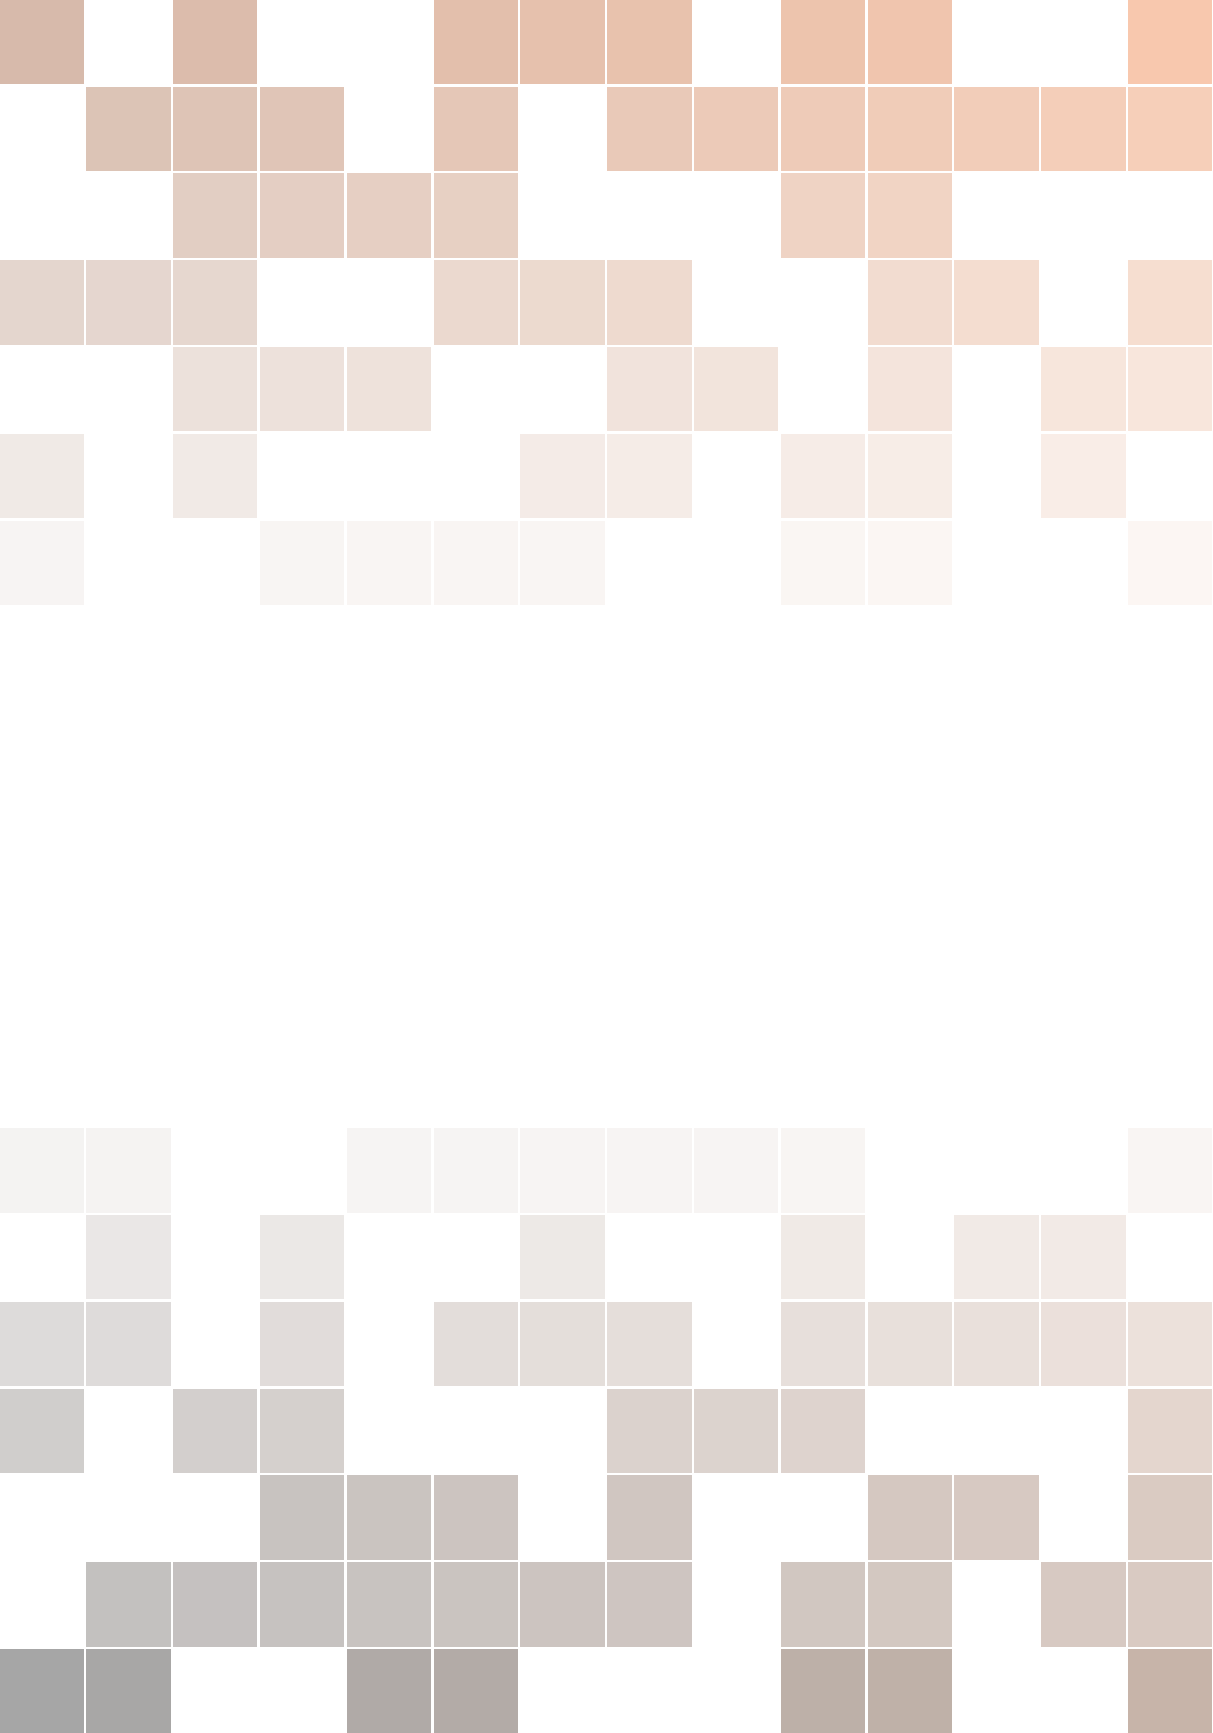
\includegraphics[width=\paperwidth]{background.pdf}};
\draw (current page.center) node [fill=ocre!30!white,fill opacity=0.6,text opacity=1,inner sep=1cm]{\Huge\centering\bfseries\sffamily\parbox[c][][t]{\paperwidth}{\centering 知识点笔记 \\[15pt] % Book title
{\Large 数学}\\[20pt] % Subtitle
{\huge Delta1037}}}; % Author name
\end{tikzpicture}
\vfill
\endgroup

%----------------------------------------------------------------------------------------
%	COPYRIGHT PAGE
%----------------------------------------------------------------------------------------

\newpage
~\vfill
\thispagestyle{empty}

\noindent Copyright \copyright\ 2022 Delta1037\\ % Copyright notice

\noindent \textsc{Published by Self}\\ % Publisher

\noindent \textsc{web: www.delta1037.cn}\\ % URL

\noindent \textsc{mail: geniusrabbit@qq.com}\\ % URL

\noindent Licensed under the Creative Commons Attribution-NonCommercial 4.0 Unported License (the ``License''). You may not use this file except in compliance with the License. You may obtain a copy of the License at \url{https://creativecommons.org/licenses/by-nc-sa/4.0/}. Unless required by applicable law or agreed to in writing, software distributed under the License is distributed on an \textsc{``as is'' basis, without warranties or conditions of any kind}, either express or implied. See the License for the specific language governing permissions and limitations under the License.\\ % License information, replace this with your own license (if any)

\noindent \textit{First printing, January 2022} % Printing/edition date

%----------------------------------------------------------------------------------------
%	TABLE OF CONTENTS
%----------------------------------------------------------------------------------------

%\usechapterimagefalse % If you don't want to include a chapter image, use this to toggle images off - it can be enabled later with \usechapterimagetrue

\chapterimage{chapter_head_1.pdf} % Table of contents heading image

\pagestyle{empty} % Disable headers and footers for the following pages

\tableofcontents % Print the table of contents itself

\cleardoublepage % Forces the first chapter to start on an odd page so it's on the right side of the book

\pagestyle{fancy} % Enable headers and footers again

% 对于自动转换部分的说明
% 1、按照chapter对知识点进行分类
% 2、每一个知识点构建成一个section
% 3、一个知识点里如果包含子内容,构建成subsection
% 4、index构建成索引
%%%%%%%%%%%%%%%%%%%%%%%%%%%%%%%%%%%%%%%%%%%%%%%%%%%%%%%%%%%%%%%%%%%%%%%%%%%%%%%%%%%%%%%%%
%----------------------------------------------------------------------------------------
%	PART 1 微积分部分
%----------------------------------------------------------------------------------------
\part{微积分}
%----------------------------------------------------------------------------------------
%	CHAPTER 1 函数与极限
%----------------------------------------------------------------------------------------
\chapterimage{chapter_head_2.pdf}
\chapter{函数极限连续}

\section{函数极限连续的注意点}\index{函数极限连续的注意点}

1、单调不一定是连续的:如果出现间断点,但间断点处符合单调趋势,则整体也是单调的

2、振荡的无穷不是无穷大:函数在某个点的去心邻域虽然无界,但是函数在该点的极限不是无穷大

3、导数的定义式与洛必达:对于导数的定义式使用洛必达(即函数在去心邻域可导),则在心处函数是连续的,左右导数相等(这两个条件也可以反向说明去心邻域可导)

4、极限趋近方向:取极限时注意趋近的值的符号,在对变量进行平方和合并到根号内部时特别注意

5、对于两个函数乘积的极限:如果两个函数的极限都不存在,乘积的极限可能存在(某些影响因子抵消了);如果两个函数其中一个极限存在,另一个极限不存在,乘积的极限可能存在,或者不存在(主要看极限不存在的影响因子是否能被极限存在的多余的影响因子抵消)

6、去心邻域无穷个点无定义不存在极限:如果在去心邻域内有无穷个点没有定义,则谈不上取极限,极限也是不存在(极限不存在的情况之一(其它有无穷,振荡))

\section{已知极限的求解}\index{已知极限的求解}



\subsection{已知极限求另一有关的极限}\index{已知极限的求解!已知极限求另一有关的极限}

1、方法一:利用极限与无穷小的关系,由题设条件去掉极限符号,解出来$ f(x) $,代入到欲求的极限式并求解

2、方法二:由已知极限出发,推导出欲求极限的一些有用的结果,或者将欲求的极限凑成已知极限的表示形式

注意:去掉极限符号时注意添加无穷小量并将无穷小量跟随计算(大题需要添加对无穷小量的说明)



\subsection{已知极限求参数}\index{已知极限的求解!已知极限求参数}

1、泰勒公式法:利用佩亚诺余项泰勒公式将函数展开,(有时需要用求解极限的方式化简)直接求解待定参数(当泰勒公式不是现成的,必要时可以推导函数的泰勒级数展开式)

2、洛必达法则法:利用洛必达法则,每一步需要对参数进行讨论,满足一定的条件才可以继续用洛必达,未知参数的值可以用满足的条件进行求解(因为极限存在,所以洛必达法则条件必定满足)

3、先化简再求值:利用求解极限的方式将极限进行化简,根据极限的值的类型求解参数

注意:有时对未知参数的值进行讨论

\section{极限存在性证明与求解}\index{极限存在性证明与求解}



\subsection{单调有界定理证明极限的存在性}\index{极限存在性证明与求解!单调有界定理证明极限的存在性}

1、数列(函数)单调减少且有下界,则极限存在并大于下界(界限可能太靠下了)

2、数列(函数)单调增加且有上界,则极限存在并小于下界(界限可能太靠上了)



\subsection{利用夹逼定理求解极限}\index{极限存在性证明与求解!利用夹逼定理求解极限}

1、使用准则:不要改变起主要作用的n的最高次项,放大缩小之后的极限相等(难点)

\section{函数的有界性讨论}\index{函数的有界性讨论}



\subsection{有界的判定}\index{函数的有界性讨论!有界的判定}

1、有界判定定理:如果函数在闭区间上连续,则函数在闭区间内有界(推论:如果函数在开区间上连续,并且两端的内侧的极限都存在,则函数在开区间内有界,开区间为无穷时也成立)(运算:有界之和、积为有界函数)

2、函数与导数有界的关系:闭区间上,导函数和原函数均有界:$ f^{\prime}(x) $在区间上有界 ⇒ $ f(x) $在区间上有界,其余有界情况均不成立(拉格朗日中值定理与绝对值放缩来证明)

3、函数与导数无界的关系:闭区间上,导函数和原函数均无界:$ f(x) $在区间上无界 ⇒ $ f^{\prime}(x) $在区间上无界,其余无界情况均不成立

4、极限表述形式:邻域内有界(指定点的极限);大于指定范围时有界(无穷远处的极限);极限趋近于无穷,则无界;极限无穷振荡,也是无界,不等同于无穷



\subsection{判定特殊情况}\index{函数的有界性讨论!判定特殊情况}

1、三角函数取特殊趋近值(不同的趋近方式):三角函数等于$ (-1,1) $之间的值时有无穷个点,导致取0值时或者取非0值时得到的极限有不同的结果

注意:无穷小与无穷大的描述(无穷大与无穷小均为单一的值)

注意:区分无穷振荡型与无穷大(无穷振荡型并非是极限无穷大)

\section{函数的间断与连续}\index{函数的间断与连续}

1、连续:区间连续表示区间内的每一点都连续

2、间断:第一类间断点(可去间断点<左右极限相等但是在点处不连续>、跳跃间断点<左右极限存在但不相等>),第二类间断点(无穷间断点<极限为无穷>、振荡间断点<无限的振荡>)

3、判断函数或者复合函数(先复合)的间断点类型:求解点处两侧的极限值和点处的值

4、极限定义式形式:判断由极限形式定义的函数的连续性或者间断点类型,先求出函数的表达式

5、找间断点(特殊点):分母为0的点,分母是三角函数为0的点,定义域的边界;化简式子;判断间断点的类型

注意:点连续邻域内不一定连续(比如狄利克雷函数)

注意:前提都是去心邻域有定义(去心邻域是一个双边的概念)

备注:复合函数的间断点消失的情况(函数的平方,绝对值都可以抹掉值域的正负性;复合内层的函数的值域不包含外层函数的间断点定义域部分,啪,间断点没了)

\section{求分段复合函数}\index{求分段复合函数}

1、分段过渡:写出中间变量的值域范围,按照外层函数的定义域范围,分段过渡到外层函数的自变量变化范围(定义域范围)

\section{极限特例}\index{极限特例}



\subsection{分类讨论的情况}\index{极限特例!分类讨论的情况}

1、含有$ |x| $,$ x $趋近于0,区分$ 0^+ $和$ 0^- $,进行讨论

2、含有$ e^{\frac{1}{x}} $,$ x $趋近于0,区分$ 0^+ $和$ 0^- $,进行讨论(同除某一个项,或者提公因式判断)

3、含有取整函数$ [x] $,$ x $趋近于整数



\subsection{常用的极限等式}\index{极限特例!常用的极限等式}

设$ \alpha>0, \beta>0 $

1、$ \lim _{x \rightarrow+\infty} \frac{\ln ^{\beta} x}{x^{\alpha}}=0 $

2、$ \lim _{x \rightarrow+\infty} \frac{x^{\alpha}}{\mathrm{e}^{\beta x}}=0 $

3、$ \lim _{x \rightarrow 0^{+}} x^{\alpha} \ln ^{\beta} x=0 $

\section{单调性相关}\index{单调性相关}



\subsection{单调性的判断}\index{单调性相关!单调性的判断}

1、定义、作差、作商:用于函数不可导时的判定;用于判断数列的单调性,在证明数列的收敛时判断数列是否是单调的

2、求导:利用导数的值在区间内的正负性进行判定(判断单调性时,不仅要关注极值点的值,也要关注端点的值,从而判断原函数的起始点和落脚点在哪里,判断原函数的整体走势)

3、复合函数单调性:同增异减

注意:单调不一定是连续的(可以用来构造反例)

注意:多个不连续区间具有相同单调性,需要用“,”或者“和”连接(单调区间的表示)

注意:区分”在区间上单调递增“和”单调递增区间是XXX“(前者可能是一个单调递增区间,后者是所有的单调递增区间)



\subsection{单调性的应用}\index{单调性相关!单调性的应用}

1、根据值域上两点值的关系,和函数的单调性,得到定义域上这两点之间的关系(即大小关系)(平常都是用定义域和单调性来判断定义域上两点的值域上的关系,这里反向推导了)



\subsection{单调性与导数}\index{单调性相关!单调性与导数}

1、导数与增函数:导数大于0,只有个别处导数为0不影响整体的增函数特性

\section{极限表示的函数的表达式}\index{极限表示的函数的表达式}

1、找影响因子(高次项等):先判断在定义域上其中哪个项在极限的求解中占主要成分

2.1、提影响因子:将其中起作用的影响因子提取出来,求解剩余部分的极限

2.2、将影响因子以外的进行放缩:利用夹逼定理(夹逼定理放缩就是不改变起主要作用的项),整个函数大于该单独的项,并小于其它所有项等于该项的值(依据实际的条件进行放缩)

放缩样例:$ <font color=purple>\sqrt[n]{|x|^{3 n}}<\sqrt[n]{1+|x|^{3 n}} \leqslant \sqrt[n]{2|x|^{3 n}}=\sqrt[n]{2}|x|^{3}</font> $

备注:当函数的表达式是用极限的形式表示时,需要先求出函数的表达式(must),再根据题目进行别的求解(判断函数的性质等)

\section{复合函数极限}\index{复合函数极限}

1、复合函数极限运算定理:设$ \lim_{x \rightarrow x{0}} \varphi(x)=u_{0} $, 且存在$ x=x_{0} $的某去心邻域$ \dot{U}\left(x_{0}\right) $, 当$ x \in \dot{U}\left(x_{0}\right) $时$ \varphi(x) \neq u_{0} $(附近没有别的等于极限$ <font color=purple>u_{0}</font> $的点,排除振荡情况;如果$ <font color=purple>u_{0}</font> $的值为无穷大,则可认为可排除振荡的情况,即无条件存在$ <font color=purple>\varphi(x) \neq u_{0}</font> $), 又设$ \lim_{u \rightarrow u{0}} f(u)=A $, 则$ \lim_{x \rightarrow x{0}} f(\varphi(x))=A $

2、复合函数的单调性与复合函数的极限存在性,按照有关的收敛、单调去考虑即可(单调有界数列必存在极限)(考虑内层函数振荡)

备注:收敛是指收敛于有限值,趋近于无穷不叫收敛

\section{大题求解极限注意事项}\index{大题求解极限注意事项}

1、判断极限的类型

2、使用洛必达时,分析洛必达的使用条件(大题中每一步使用洛必达都需要验证洛必达条件)

3、验证积分为无穷:对于积分为无穷的验证表达形式,求解积分内函数的极限值,当极限存在时,设存在一个$ 0 $到该极限的中间值$ f $,当积分的上限大于某个充分大的$ T $时,积分内函数的值大于中间值$ f $,将积分的区域分解成$ 0→T $和$ T→无穷 $两部分,前一部分为有限值,后一部分利用放缩,求解出来值为无穷,从而证明积分的值为无穷<复习全书 P17完整步骤>

4、洛必达法则无穷/无穷型:当分母满足为无穷值时,无论分子是什么(存在、不存在),洛必达法则的结论仍然成立(推广式)

\section{奇偶性的判断}\index{奇偶性的判断}

1、利用定义:利用奇偶性的定义进行讨论

2、导函数的奇偶性:导函数的奇偶性根据被求导的函数的奇偶性进行讨论(奇导为偶,偶导为奇,偶导的零点可能不存在)

3、原函数的奇偶性:原函数的奇偶性通过变上限积分$ F(x)=F(0)+\int_{0}^{x} f(t) \mathrm{d} t $讨论(奇函数的原函数一定是偶函数,偶函数的原函数不一定是奇函数,借用$ <font color=purple>F(x)=F(0)+\int_{0}^{x} f(t) \mathrm{d} t</font> $来进行讨论,可以看出$ <font color=purple>F(0)</font> $的值不会影响偶函数的特性,但是会影响奇函数的特性(因为0处必须等于0))

4、积分的奇偶性判断:对积分求导

\section{求函数的极限方法}\index{求函数的极限方法}

1、化简:不完全平方形式(有理化;分母补1);无穷多项时先对无穷多项求和(无穷多项相加可能会出现更高次项);幂指函数指数化(整体部分都可用,即可以对部分进行指数化)(不要把指数的底给丢了);三角函数化简(升幂,降幂,合并);提公因式(无穷减无穷形式,指数函数,幂函数)(属于整体的因式);提出为有限值的乘积项(极限存在且不为0的因式按照乘积法则提取出来);极限四则运算(和差商积的极限两个极限都要存在,且商的分母极限值不为零);有界函数与无穷小乘积为无穷小

2、等价无穷小替换:对整体的因式操作,等价无穷小的条件是$ x $趋于0

3、洛必达法则:需要验证是否可以洛必达(去心邻域必须可导,0/0型,无穷/无穷型,洛必达的分母的导数不恒为零,求导过后极限应为有限值或者无穷就算洛必达成功(不包括振荡形式),当洛必达的求解结果是不是无穷的不存在,不能说原极限不存在,应该用别的方法),特别是大题要进行验证(带有反三角函数的大概率需要用洛必达)(对抽象函数使用洛必达时,注意验证题目是否给出了可用洛必达的条件)

4、佩亚诺余项泰勒公式:注意展开的阶数

5、夹逼定理:常用的放缩形式

6、拉格朗日函数法:判别规则(存在基形式一致的函数(或者通过加减项凑形式);复合函数特别复杂,但是复合的外层一致的情况,可以使用拉格朗日法将最外层去掉(外层函数类似$ <font color=purple>tanx</font> $,$ <font color=purple>e^x</font> $之类的))(去掉的最外层的函数的导数的极限应该存在)

7、数列和的极限:数列转积分和式(利用积分的定义)($ dx=\frac{1}{n} $,$ x=\frac{i}{n} $)

8、带变限积分的式子:规范变量(对于积分号里面的变量$ <font color=purple>x</font> $,使用拆项的办法放到积分外面;对于被积分函数里的函数$ <font color=purple>f</font> $含有变量$ <font color=purple>x</font> $使用变量代换的方式换到积分限中),使用洛必达法则去掉积分符号

9、单调有界定理:

10、导数的定义的运用:

11、部分项求解代入:对其中类似的项拎出来单独求极限,求出来如果极限存在再代入求解

备注:极限是一个两边趋近概念,讨论范围都是去心邻域;求解极限时除了佩亚诺余项泰勒公式和部分项求解代入法,不允许对一部分进行求解;

注意:求解极限注意符号问题(根据大致的值进行判断);无穷比无穷时,一般要进一步化简(同时除以某一个无穷大);使用式子替换趋于某个值的变量时,需要判断式子是不是只能趋近一边,即只能求解单边的极限

问题:单边极限的求解,也可以用无穷小替换,泰勒公式等?(待验证,如果有看到有人这么做了,可能就是对的)

\section{无穷小的比较}\index{无穷小的比较}



\subsection{无穷小比较的方法}\index{无穷小的比较!无穷小比较的方法}

1、利用商的极限的值进行比较

2、将式子使用泰勒公式展开

3、洛必达法则

4、等价无穷小的充要条件



\subsection{无穷小的分类}\index{无穷小的比较!无穷小的分类}

1、同阶无穷小

2、等价无穷小

3、高阶无穷小、低阶无穷小

4、无穷小的阶数

\section{极限的性质与应用}\index{极限的性质与应用}

1、极限的保号性:在极限的一个范围,表达式与极限的值接近(对于数列,比如当$ <font color=purple>n</font> $无穷时极限为$ <font color=purple>A</font> $,则存在一个充分大的值$ <font color=purple>N</font> $,使得大于$ <font color=purple>N</font> $的时候,数列表达式与$ <font color=purple>A</font> $的值接近(做一下放缩,变成确定的值$ <font color=purple>A_0</font> $))

2、极限的唯一性:如果极限存在,极限值必唯一

3、去极限符号:极限定义为$ \lim \frac{g(x)}{f(x)}=A $,则可以将极限符号去掉,得到$ g(x) = Af(x)+o(f(x)) $,其中$ o(f(x)) $是$ f(x) $的无穷小量(注意:对于无穷小量的描述和分解,如果$ <font color=purple>o(\Delta x)</font> $为$ <font color=purple>\Delta x</font> $的无穷小量,则$ <font color=purple>o(\Delta x) \sim \varepsilon·\Delta x</font> $,其中$ <font color=purple>\varepsilon</font> $为无穷小量)

\section{数列极限(和式或者递推式)}\index{数列极限(和式或者递推式)}



\subsection{求解数列的极限-递推形式}\index{数列极限(和式或者递推式)!求解数列的极限-递推形式}

1、单调有界准则(递推式包含两项):先利用已知条件证明数列是有界的(可以试用夹逼定理,或者放缩,归纳法),然后利用放缩证明数列两项之间的关系(单调性,除了$ <font color=purple>u_{n+1}-u_{n}</font> $,也可以用$ <font color=purple>\frac{u_{n+1}}{u_{n}}</font> $),由单调有界性证明界限存在,然后假设极限的值,代入到已知关系式中求解到极限的值(先证明存在,然后设值求解)

2、猜测极限并证明(递推式包含两项):在可以事先猜出极限值的前提下计算出极限$ \lambda $,然后证明极限确实是这个值(验证$ <font color=purple>\lambda_n</font> $是否是收敛于$ <font color=purple>\lambda</font> $,可以转化为相减趋近于0,中间可以用夹逼定理之类的求解方式,因为$ <font color=purple>\lambda</font> $是个抽象值,而结果需要明确的趋近于0,所以需要将式子放缩,将$ <font color=purple>\lambda</font> $放到可以明确求解的部分)<参考 复习全书 P29>(特征:使用递推式或者迭代式表示出数列的各个项的值,极限式类似为$ <font color=orange>lim_{n \rightarrow \infty}\lambda_n</font> $)

3、逐项相加抵消求解通项公式(递推式包含三项):求解数列的递推式,如果为$ x_{n+1}-x_{n}=q(x_{n}-x_{n-1}) $的形式,则将$ x_{n}-x_{n-1} $逐项相加,由于$ x_{n}-x_{n-1} $是公比为q的等比数列,所以$ x_{n}-x_{n-1} $的值是知道的,逐项相加可以互相抵消得到$ x_{n} $的式子

4、证明项的正负性:将递推的两项分离到两边,然后利用归纳法证明



\subsection{求解数列的极限-其它形式}\index{数列极限(和式或者递推式)!求解数列的极限-其它形式}

1、夹逼定理:(可放缩形式)

2、数列转函数讨论(一项表示通项公式):对于一般的数列,如果可以明确写出使得$ u_{n}=f(n) $的函数时,可以利用函数来转换成讨论函数的极限(这是离散转连续的一种方式,如果是连续转离散,不同的路径可能会导致结果不一致,如在三角函数$ <font color=purple>sin(1/x),x \rightarrow 0</font> $中)



\subsection{求解数列和的极限-积分和式形式或者可转化成积分和式形式}\index{数列极限(和式或者递推式)!求解数列和的极限-积分和式形式或者可转化成积分和式形式}

特征(用来替换和发现积分和式形式):$ dx=\frac{1}{n} $,$ x=\frac{i}{n} $

样例:$ \lim _{n \rightarrow \infty} \sum_{i=1}^{n} f\left(\frac{i}{n}\right) \cdot \frac{1}{n}=\int_{0}^{1} f(x) \mathrm{d} x $

形式及方案:

1、和式形式:直接以和式进行表示的极限,并且有积分和式特征

2、乘积形式:n个因式的积,常指数化之后指数部分转换成和式求解

注意:序列变量$ <font color=purple>i</font> $(也是和式的限制变量)的变化从$ <font color=purple>1-n</font> $,或者$ <font color=purple>0-(n-1)</font> $

备注:有时需要进行放缩(夹逼定理)才能转换成积分和式(比如两项相乘而不是n项相乘)

备注:有时和式的两项是分离的,需要进行并项处理




%----------------------------------------------------------------------------------------
%	CHAPTER 2 一元微分
%----------------------------------------------------------------------------------------
\chapterimage{chapter_head_2.pdf}
\chapter{一元微分}

\section{导数的注意点}\index{导数的注意点}



\subsection{概念区分问题}\index{导数的注意点!概念区分问题}

1、区分点可导与邻域可导:高一阶的导数在某个点存在,说明低一阶的导数在该点邻域连续;当没有说函数的(去心)邻域可导时,不能对函数求导数,也就是不能对该函数使用洛必达法则,求解极限只能凑成导数的定义形式

2、点可导可推出邻域连续:已知某一点可导可以获得的隐含条件,包括函数在该点的邻域内连续(左右极限相等并等于该点的值),函数在该点的左右导数相等

3、点处连续不一定可导:尖锐的点,左右导数不相等

4、点处可导但是在邻域不一定可导:在点处可导但是邻域的导数在该点的极限不一定存在,因为邻域的导数可能会出现振荡的成分,导致导数不存在(即点处可导,邻域导数在点处的极限不一定等于点处的导数(振荡起来了))(一个点处的导数不可以推导出邻域的单调性,但是可以根据极限的保号性(导数的定义与极限的定义)推出邻域的值与导数点值的大小关系)

5、两个函数和的导数存在推不出两个函数的导数分别都存在:函数相加会损失掉一部分信息(损失掉无穷或者振荡的部分)

6、极值点:是去心邻域内最大的点,所以即使函数不连续也可以,只要是最大的就行了

7、一元函数点处可导可以推知点处可微,且微分和导数相关联:$dy=f^{\prime}(x)dx$

8、大题规范:描述参数方程的单调性和拐点时,$t$的范围和对应$x$的范围一起描述

9、反函数存在的条件:函数严格单调

10、单调函数在闭区间内是没有极值点的,因为不存在在去心邻域内的最大点



\subsection{求导容易出现的问题}\index{导数的注意点!求导容易出现的问题}

1、求导未求尽:对于$arctan(f(x))$之类的函数求导忘记对$f(x)$求导;对于$(1+f(x))^{a}$之类的函数求导忘记对$f(x)$求导;对于$\sqrt{(1+f(x))}$之类的函数求导忘记对$f(x)$求导(与幂形式是一样的,可以转换)(不要忘记指数部分带来的阶乘)

2、幂指函数求导:转换成指数函数求导,不要忘记指数项,求导要求完整

\section{导数与微分}\index{导数与微分}



\subsection{导数的定义}\index{导数与微分!导数的定义}

1、导数定义式1:$\lim _{x \rightarrow x_{0}} \frac{f(x)-f\left(x_{0}\right)}{x-x_{0}}=f^{\prime}\left(x_{0}\right)$

2、导数定义式2:$\lim _{\Delta x \rightarrow 0} \frac{f\left(x_{0}+\Delta x\right)-f\left(x_{0}\right)}{\Delta x}=f^{\prime}\left(x_{0}\right)=\left.\frac{\mathrm{d} f(x)}{\mathrm{d} x}\right|_{x=x_{0}}$

3、高阶导数定义:高阶导数的定义式与导数的定义式类似

4、在点处可导:左右导数均存在且相等

注意:定义中的$\Delta x$是可正可负的,是从两边趋近的,如果区分了正负就是左右导数(如果需要对$\Delta x$进行函数形式替换,需要判断函数形式的正负性,判断替换之后得出的是左右导数中的一个,还是点处的导数)

注意:在一点导数存在是指左右导数均存在且相等



\subsection{不可导}\index{导数与微分!不可导}

1、判断不可导点:绝对值函数与非绝对值函数下相乘,求解出所有的零点,判断哪些是只有在绝对值函数内的(只有绝对值函数内的零点才是不可导点,其余的会和绝对值函数外的零点合并,变成可导点)



\subsection{微分和增量的关系}\index{导数与微分!微分和增量的关系}

1、增量与微分相差一个变量的一阶无穷小,可以用拉格朗日余项泰勒公式关联起来$\Delta y-\mathrm{d} y=\frac{1}{2} f^{\prime \prime}(\xi)(\Delta x)^{2}$(大于零或者小于0取决于二阶导的正负性,可以使用拉格朗日余项泰勒公式证明)

\section{特殊函数形式的求导}\index{特殊函数形式的求导}

1、参数式函数的求导:对于一阶导,$x$和$y$分别对$t$求导,然后相除;对于二阶导,将一阶导对$t$求导,除以$x$对$t$求导(理解推导过程)

2、极坐标函数的求导:将极坐标形式转换成$\theta$的参数式,采用参数式函数的求导方式(参数方程为$r=r(\theta)$;转换成$\theta$为参数的参数方程是$\left\{\begin{array}{l}x=r(\theta) \cos \theta \\y=r(\theta) \sin \theta\end{array},(\theta \text { 为参数 })\right.$)

3、隐函数的求导:对于一阶导,将隐函数中$y$视为$x$的函数,将函数的两边同时对$x$求导,得到$dx/dy$的式子,解出来即可(也可以用隐函数求导法则,不要忘记负号即可);对于二阶导,将求得的一阶导继续对x求导,并将求解出来的一阶导代入,得到不含导数的二阶导

4、反函数的求导:一阶导将微分形式颠倒即是$x$对$y$的导数;二阶导对一阶导继续求对$y$的导数,转换成求对$x$的导数,并与$x$对$y$的导数相乘(链式法则,当求导变量与函数的自变量不对等时,使用链式法则将不对等变量转移,例如将x的函数对y求导,先将x的函数对x求导,然后与x对y求导相乘)(可以由已知函数的导数求解反函数的导数,能求解的反函数的导数最高阶数与已知函数导数的最高阶数一致)

5、幂函数的求导:转换成指数形式求导

6、绝对值的导数:

6.1、去绝对值分类讨论:讨论绝对值内的正负性,分类讨论,去掉绝对值;或者将整体收缩到绝对值内,如下的函数在一点为0的特殊情况

6.2、绝对值的处理情况:当函数在一点为$f(a)=0$时,有$|f(x)|-|f(a)|=|f(x)|=|f(x)-f(a)|$,将导数定义全部转入到绝对值内,然后分成左右趋近两种情况讨论

\section{按照定义求解一点的导数}\index{按照定义求解一点的导数}



\subsection{明确的由已知可得需要用定义求解}\index{按照定义求解一点的导数!明确的由已知可得需要用定义求解}

1、先讨论连续性:不连续的函数一定不可导

2、利用定义求解该点处的左右导数:如果两边函数相同,则利用一次定义式即可求解,定义式极限存在则导数存在;如果两边函数不同,则需要分别对两边进行定义式求左右导数,左右导数都存在且相等则导数存在



\subsection{隐含的需要已知式子凑成包含定义式的式子}\index{按照定义求解一点的导数!隐含的需要已知式子凑成包含定义式的式子}

1、确定求导位置:凑成在指定点的导数定义式

2、凑定义式:通过对式子进行变换,凑出定义式(分离出来导数的定义式和另一个简单的形式相乘,转换成求解两个极限式相乘)

注意:将极限进行拆分时,拆分后的两个极限需要都存在

\section{可导与极限}\index{可导与极限}



\subsection{讨论由极限式定义的函数的导数}\index{可导与极限!讨论由极限式定义的函数的导数}

1、先求解函数的表达式

2、再讨论函数导数的情况,利用定义或者求导



\subsection{已知函数在某一点可导,求解与此相关的极限或者参数}\index{可导与极限!已知函数在某一点可导,求解与此相关的极限或者参数}

1、当分数形式存在极限时的可推导内容:当分数形式存在极限时,如果分子或者分母一边为含有未知函数的式子,则含有未知函数的一边与另一边同阶,根据分数极限的值,可以推断含有未知函数的一边的等价形式(系数*阶数幂+无穷小,即去极限符号);特别的,不含未知参数的一边为0,且整体极限不为0,则含参数的一边极限也是0

\section{求解n阶导数}\index{求解n阶导数}

1、简单的有理式直接拆项(简单拆项):对幂函数求导时,注意指数部分会导致求导之后出现阶乘(出现$n!$)

2、泰勒级数+0处$n$阶导(0点展开):如果式子可以套用常用的泰勒级数(都是0点处的展开)展开,则可以直接展开,然后求解第$n$次幂的系数即可(注意泰勒级数的系数中除了导数之外分母还有一个$n!$,在对级数进行求导时,与$x$的幂阶数进行抵消,当求导至$x$的幂为0阶时,式子就剩下了泰勒级数展开点的$n$阶导数值)

3、幂级数与泰勒级数综合(任一点展开):将式子展开为幂级数(在题目要求求解某一点的导数时):幂级数展开式($\varphi(x)=\sum_{n=0}^{\infty} a_{n}\left(x-x_{0}\right)^{n}$),泰勒级数展开($\varphi(x)=\sum_{n=0}^{\infty} \frac{1}{n !} \varphi^{(n)}\left(x_{0}\right)\left(x-x_{0}\right)^{n}$),对应关系($\varphi^{(n)}\left(x_{0}\right)=n ! a_{n}, \quad(n=0,1, \cdots)$)(注意不要忘记幂级数的系数需要乘$n!$)

4、预处理:如果是复杂的函数(arctan),先求导一次之后,展开成幂级数,再将幂级数积分得到原函数的幂级数(求解原函数时注意$f(x)=f(0)+\int_{0}^{x} f^{\prime}(t) \mathrm{d} t$,补充一点是为了让0处改式子也成立)

\section{函数特征判断}\index{函数特征判断}



\subsection{驻点}\index{函数特征判断!驻点}

1、驻点为一阶导为0的点(极值点不一定是驻点,因为极值点可能不存在导数)

备注:驻点是一个横向坐标($x=x_0$)

注意:驻点一定是平滑的;驻点处可能没有方向的变换(即单调)



\subsection{极值点}\index{函数特征判断!极值点}

0、极值点定义:邻域内存在一点的值大于等于或者小于等于其它的值(邻域内需要有定义,无穷值不算有定义;邻域是双边的,如果只有一边有定义,则也不叫有定义)

1、第一充分条件:函数在点处连续,点处去心邻域内可导(点处可能不可导:点处为尖锐的点),两侧导数数值反号(这种类型包括尖锐点)(备注:若函数连续,且左右导数存在,$f(x_0)$为极值,未必存在左右导数反号,例如常函数的极值)

2、第二充分条件:函数在点处去心邻域存在二阶导,点处一阶导为0,二阶导不为0(注意二阶导可能只有一点,点处二阶导存在可以推知一阶导点邻域内连续,函数在该点邻域内也连续)(二阶导为0,不一定不是极值点,比如x的三次方)

3、可导点极值必要条件:如果函数在一点处取得极值,并且该点导数存在,则导数一定为0,反之不成立

备注:极值点是一个横向坐标($x=x_0$);极值是纵向坐标($y=f(x_0)$)

注意:极值点也可能是尖锐的(连续但是不可导的点)

注意:极值点是去心邻域内最大的点,所以即使函数不连续也可以,只要是最大的就行了;单调函数在闭区间内是没有极值点的,因为不存在在去心邻域内的最大点



\subsection{最值}\index{函数特征判断!最值}

最值定义:区间上,存在一点的值大于等于或者小于等于其它区间上所有的值(区间上需要有定义,无穷值不算有定义)

1、找到所有的驻点和不可导的点(尖锐的点和端点)

2、比较所有的点的值

备注:最值是一个纵向坐标($f(x_0)$)

注意:若区间内只有一个极值点,该极值点必是最大或最小值

注意:讨论应用问题最值时注意判定函数在区间内是否可导(注意应用的实际情况)



\subsection{拐点}\index{函数特征判断!拐点}

1、二阶导判定:去心邻域二阶可导(注意:点处可能不可导会有出现尖锐点的情况),且点处左右二阶导数反号→是拐点(点的两边不连续也行,只要凹凸性相反就行了)

2、三阶导判定:二阶导为0,三阶导不为0的点也是拐点(三阶导不为0是为了确定二阶导在该点邻域是反号)

3、邻近域判断:如果某个点的临近域的凹凸性相反,则该点是拐点

4、更高阶导判断:如果函数某一点处n阶导不为零,n阶一下都是零,则当n为奇数时,是拐点,偶数时不是拐点

备注:拐点是一个二维坐标($(x_0,y_0)$)

注意:拐点处二阶导为0或者不存在

注意:一点是极值点就不是拐点,是拐点就不是极值点



\subsection{凹凸性}\index{函数特征判断!凹凸性}

1、二阶导判断:区间上二阶导大于等于0(小于等于0)(注意:不在某一个区间上取等)→凹的(凸的);可以理解为二阶导大于0,导数增加越来越快导致图像下凹,或者二阶导小于0,导数增加越来越慢导致图形上凸

2、三阶导判断:画图转成二阶导判定(需要有一些辅助定量的点才能画图)



\subsection{曲率、曲率圆、曲率半径}\index{函数特征判断!曲率、曲率圆、曲率半径}

1、曲率计算公式(注意:曲率与二阶导符号无关):$k=\frac{\left|y^{\prime \prime}\right|}{\left(1+y^{\prime 2}\right)^{3 / 2}}$

2、曲率半径:$R=\frac{1}{k}=\frac{\left(1+y^{\prime 2}\right)^{3 / 2}}{\left|y^{\prime \prime}\right|}$

3、曲率中心坐标:$(\alpha=x-\frac{y^{\prime}\left(1+y^{\prime 2}\right)}{y^{\prime \prime}}, \beta=y+\frac{1+y^{\prime 2}}{y^{\prime \prime}})$(曲率中心由点处的法线方程和曲率半径求得,相应的可以得到曲率圆方程)

注意:如果题目给出了曲率圆方程,可以通过求解曲率圆方程的导数获得曲线的导数(一阶和二阶导都是相等的)(可以避免讨论)

注意:如果使用曲线求导,会因为曲率计算公式中有绝对值的存在而导致参数需要讨论(讨论绝对值)



\section{求渐近线}\index{求渐近线}



\subsection{XY坐标系式子的求解:(备注:一共需要验证6种情况,但是在无穷的位置水平和斜渐近线只能存在一个(同一边的无穷))}\index{求渐近线!XY坐标系式子的求解:(备注:一共需要验证6种情况,但是在无穷的位置水平和斜渐近线只能存在一个(同一边的无穷))}

1、水平渐近线:正无穷和负无穷的极限值,$\lim _{x \rightarrow \infty} f(x)=b$(注意正无穷和负无穷如果极限值一样只能算一条)(注意:包含正无穷和负无穷)

2、铅直渐近线:趋近于某个值时,极限不存在(表现为存在$x_{0}$,  使$\lim_{x \rightarrow x{0}^{-}} f(x)=\infty$ (或$\lim_{x \rightarrow x{0}^{+}} f(x)=\infty$);先由观察法得知特殊点(分母为0,对数的真数为0处)(注意:包含左趋近和右趋近)

3、斜渐近线:($\lim _{x \rightarrow+\infty} \frac{f(x)}{x}=a$)趋近于无穷的极限为斜率a,($\lim _{x \rightarrow+\infty} ({f(x)}-{ax})=b$)趋近于无穷的极限即为截距b(获得y=ax+b,斜渐近线方程)(注意:包含正无穷和负无穷)(当只有斜率存在并且截距存在时才有斜渐近线,如果仅有斜率存在但是截距为无穷或者振荡形式,则渐近线是不存在的)



\subsection{参数方程的求解:(找$x$无穷的点和$y$无穷的点)}\index{求渐近线!参数方程的求解:(找$x$无穷的点和$y$无穷的点)}

1、水平渐近线:找一个使得$x$趋近于无穷时的$t_0$点(特定值或者无穷),求解$t$趋近于$t_0$时$y$的值

2、铅直渐近线:找使$y$趋近于无穷并且$x$是有限值的点$t_0$

3、斜渐近线:找一个使得$x$趋近于无穷时的$t_0$点(特定值或者无穷),求解$\lim _{t \rightarrow t_0} \frac{y(t)}{x(t)}=a$,$\lim _{t \rightarrow t_0} ({y(t)}-{ax(t)})=b$,(获得$y=ax+b$,斜渐近线方程)(当只有斜率存在并且截距存在时才有斜渐近线,如果仅有斜率存在但是截距为无穷,则渐近线是不存在的)

\section{中值、不等式、零点问题的基本定理}\index{中值、不等式、零点问题的基本定理}

1、费马定理:可导条件下的极值的必要条件,即可导时,极值位置的导数为0

2、罗尔定理:函数$f(x)$在闭区间$[a,b]$上连续,在开区间$(a,b)$内可导,并且两端值相等$f(a)=f(b)$,则至少存在一点$\xi \in(a, b)$,使得$f^{\prime}(\xi)=0$(相同高度的点中间存在水平切线)

3、拉格朗日中值定理:函数$f(x)$在闭区间$[a,b]$上连续,在开区间$(a,b)$内可导,则至少存在一点$\xi \in(a, b)$,使得$f(a)-f(b)=f^{\prime}(\xi)(a-b)$(另一种常用形式:在定理条件下$x_0$和$x$是区间$[a,b]$上的任意两点,至少存在一点$\xi$在$x_0$和$x$之间,使得$f(x)=f\left(x_{0}\right)+f^{\prime}(\xi)\left(x-x_{0}\right)$成立,令$\theta = \frac{\xi - x_0}{x-x_0}$,其中$0< \theta < 1$,则拉定又可以写成$f(x)=f\left(x_{0}\right)+f^{\prime}\left(x_{0}+\theta\left(x-x_{0}\right)\right)\left(x-x_{0}\right)$,其中$f^{\prime}\left(x_{0}+\theta\left(x-x_{0}\right)\right)$是$f^{\prime}(\xi)$的另一种表达)

4、柯西中值定理:函数$f(x),g(x)$在闭区间$[a,b]$上连续,在开区间$(a,b)$内可导,且$g(x)\ne 0,x \in(a, b)$,,则至少存在一点$\xi \in(a, b)$,使得$\frac{f(b)-f(a)}{g(b)-g(a)}=\frac{f^{\prime}(\xi)}{g^{\prime}(\xi)}$

5、泰勒定理:函数$f(x)$在闭区间$[a,b]$上有$n$阶连续导数,在开区间$(a,b)$内具有$n+1$阶导数($n+1$阶是为了表示$R_{n}(x)$),$x_0$和$x$是区间$[a,b]$上的任意两点,至少存在一点$\xi$在$x_0$和$x$之间,使得$f(x)=f\left(x_{0}\right)+\frac{f^{\prime}\left(x_{0}\right)}{1 !}\left(x-x_{0}\right)+\frac{f^{\prime \prime}\left(x_{0}\right)}{2 !}\left(x-x_{0}\right)^{2}+\cdots+\frac{f^{(n)}\left(x_{0}\right)}{n !}\left(x-x_{0}\right)^{n}+R_{n}(x)$,其中$R_{n}(x)=\frac{f^{(n+1)}(\xi)}{(n+1) !}\left(x-x_{0}\right)^{n+1}$(如果将条件减弱为函数$f(x)$在$x=x_0$处(只有一点)有$n$阶导数(这意味着在$x=x_0$的邻域内具有连续的$n-1$阶导数,即$f^{(n-1)}(x)$在$x=x_0$处连续,$x$为$x_0$邻域内充分小的邻域内的任意一点,有$f(x)=f\left(x_{0}\right)+\frac{f^{\prime}\left(x_{0}\right)}{1 !}\left(x-x_{0}\right)+\cdots+\frac{f^{(n)}\left(x_{0}\right)}{n !}\left(x-x_{0}\right)^{n}+R_{n}(x)$,其中$R_{n}(x)=o\left(\left(x-x_{0}\right)^{n}\right)\left(\lim_ {x \rightarrow x{0}} \frac{o\left(\left(x-x_{0}\right)^{n}\right)}{\left(x-x_{0}\right)^{n}}=0\right)$,这就是佩亚诺余项泰勒公式)

6、积分中值定理:

注意:如果泰勒公式中展开点为0点,则称该公式为麦克劳林公式

注意:拉格朗日中值定理时罗尔定理证明的,不能用拉定去证明罗定

注意:具有拉格朗日余项的0阶泰勒公式就是拉格朗日中值公式

注意:具有拉格朗日余项的1阶泰勒公式,就是函数的微分与增量之间的关系公式

注意:泰勒定理在不同的位置展开,$\xi$要用不同的值$\xi_n$表示

\section{不等式证明}\index{不等式证明}



\subsection{证明不等式方法}\index{不等式证明!证明不等式方法}

1、单调性的方法:首先将函数相减得到新函数(构造),如果该函数在区间内是单调的,判断两个端点的值是大于零还是小于0的,从而得到该函数的值在区间内的正负性;如果该函数在区间内分成两个区间,分别单调递增和单调递减,考虑两个端点的值和中间分界点的值,从而得到该函数在区间内的正负性(最值的方法:如果构造的函数的最小值大于等于0,则函数整体大于0;如果构造的函数的最大值小于0,则函数整体小于0)

2、拉格朗日中值公式的方法(一阶导用一次,二阶导需要拆分开用两次拉定,二阶导关键是找到一个中间值):(题目特征:$f(b)-f(a)>A(b-a)(or \ f(b)-f(a)<A(b-a))$),由$f(a)-f(b)=f^{\prime}(\xi)(a-b)$,只要证明$f^{\prime}(\xi)>A\left(\text { 或 } f^{\prime}(\xi)<A\right), \text { 当 } \xi \in(a, b)$(注意其中A是一个定值,不包括参数a、b!)(拉格朗日中值定理可以认为是对函数利用导数值进行区间(利用区间的端点)上的一种放缩)

3、拉格朗日余项泰勒公式的方法(二阶导数):(题目特征:函数二阶导存在,并且大于或者小于0),将$f(x)$在合适的$x=x_0$处展开,有$f(x)=f\left(x_{0}\right)+\frac{1}{1 !} f^{\prime}\left(x_{0}\right)\left(x-x_{0}\right)+\frac{1}{2 !} f^{\prime \prime}(\xi)\left(x-x_{0}\right)^{2}$,证明的关键是合适的$x=x_0$处展开;这种特征情况下也可能用两次拉格朗日中值定理证明



\subsection{存在某个$\xi$满足某不等式:(存在性证明,对函数特征分析找到一点即可)}\index{不等式证明!存在某个$\xi$满足某不等式:(存在性证明,对函数特征分析找到一点即可)}

1、肯定不能用的:罗尔定理,极值的必要条件(这两个定理都是求相等的,不能证不等式),单调性也不能用(单调性证明区间的值的大小,而这是要证明$\xi$满足不等式)

2、可以用的:拉格朗日中值定理(存在一阶导),拉格朗日泰勒余项公式(展开到第$n$阶就需要存在$n$阶连续导数,即开区间存在$n+1$阶导数)

函数构造:构造函数$\varphi(x)=f(x)-\left[f(a)+\frac{f(b)-f(a)}{b-a}(x-a)\right]$,$\varphi^{\prime}(x)=f^{\prime}(x)-\frac{f(b)-f(a)}{b-a}$(得到了拉格朗日中值定理的中值导数和两端斜率的式子,通过判断拉格朗日定理中$\varphi^{\prime}(x)$因题目条件出现大于0或者小于0,就可以得到拉格朗日中值定理的$\xi$的不等式)



\section{不等式的证明方法细节}\index{不等式的证明方法细节}

1、将不等式中的一个量转换成变量:转换成一个函数,转为用函数单调性的方法求解(当某一个端点是开区间时,求解该端点的极限值,构造新的补充端点值得函数讨论函数在区间上得正负性)(注意将1转换成变量时,可能需要有隐藏的变量需要转换)

2、对称性的应用:证明含有$1/u$在$(0,\infty)$区间上的单调性,先证明$(0,1)$,再利用对称性证明$(1,\infty)$,减小计算量(用变量替换。替换后形式与原式子形式一致)

3、有高阶导:用拉格朗日余项泰勒公式推导函数的值,再所证的范围上的其中一个端点展开(该点的高阶导数要尽可能地多;尽可能让不需要的项为0;容易约去的点,用于多个函数泰勒组合)

4、拉格朗日中值公式与单调性的证法是相通的:单调性可以将拉格朗日中值公式化简成$f(b)-Ab>f(a)-Aa$,构造函数$f(x)+Ax$,求导即是证明$f^{\prime}(x)-A>0$类似的问题,与拉格朗日中值公式的证明类似

5、两端值未定的规范化:假设$f(a),f(b)$的关系未定,构造函数$\varphi(x)=f(x)-\left[f(a)+\frac{f(b)-f(a)}{b-a}(x-a)\right]$,这样就有$\varphi(a)=\varphi(b)$

6、式子预处理:如果是复杂的乘式,利用求对数,将乘积形式变为和差的形式

7、罗尔定理是证明导数零点的(等式),如果题目中给出一个区间两个端点值为0的情况,用拉定在$x$(区间的中间值)和这两个值联立得到两个式子,

8、数值不等式也可以通过一些定理的形式转换,例如如果具有拉格朗日中值定理的形式,就将原数值不等式转换成了函数导数不等式的形式

注意:当不等式两边同时乘一个负值时,不等式要变号

\section{零点问题的证明(等式的证明)}\index{零点问题的证明(等式的证明)}



\subsection{至多有几个零点的证明}\index{零点问题的证明(等式的证明)!至多有几个零点的证明}

当函数的各阶导数存在时(原函数的零点存在性)

1、如果$f'(x)$没有零点,则$f(x)$至多有$1$个零点

2、如果$f'(x)$至多有1个零点,则$f(x)$至多有$2$个零点

3、如果$f'(x)$至多有k个零点,则$f(x)$至多有$k+1$个零点

4、如果$f''(x)$没有零点,则f'(x)至多有$1$个零点,$f(x)$至多有$2$个零点,$…$,依此类推

注意:该规则的方向与罗尔定理相反,规定了导数的原函数至多有多少零点(导函数正负切换与原函数跨y轴次数的关系。导函数正负切换不一定会导致原函数跨y轴(出现零点),但是如果导函数正负切换全导致了原函数跨$y$轴变化,那么这就是原函数零点最多的情况)



\subsection{零点存在性证明}\index{零点问题的证明(等式的证明)!零点存在性证明}

1、连续函数的介值定理:连续函数在区间上有最大值M和最小值m,则在区间上必存在一点使得函数值在最大值和最小值之间(闭区间)(注意:如果题目未设定函数连续,则不能用连续函数的介值定理来说明有零点或者存在某一点)

2、连续函数的零点定理:如果函数的两端的值相乘小于0,则在开区间上至少存在一点,使得函数值为0

3、利用罗尔定理(导函数的零点存在性):以下设所提到的导数存在,则有结论:如果$f(x)$有$k(k≥2)$个零点,则$f'(x)$至少有$(k-1)$个零点;$…$,$f^{(k-1)}(x)$至少有$1$个零点(求导之后,会减少零点的个数)(该规则规定了求导之后至少应该有多少个零点)(跨y轴的零点与增减性(导函数正负切换的次数)的关系,原函数零点的出现,使得两个零点之间必有一次导函数的正负切换(即导函数的零点),由于两个零点之间的导函数切换会出现大于一次的情况,所以这就是导函数零点最少的情况)

4、两种不同函数形式的存在性证明等式:想到用柯西中值定理证明;需要找到其中一个函数的导数形式

备注:罗尔定理也可以看作是导函数的零点定理,构造积分式,积分两端的值相等,即存在导函数为0,即被积分函数存在为0的点,即存在零点



\subsection{零点问题证明细节}\index{零点问题的证明(等式的证明)!零点问题证明细节}

1、当需要证明积分式中被积分函数的零点:用罗尔定理,证明积分两个端点值相同,则存在导数即被积分函数存在零点

2、有极大值大于0的曲线,判断与$x$轴的交点,需要判断两边延伸部分的正负性;极小值同理

3、零点的个数问题,可以用至多存在几个零点和至少存在几个零点进行框定(夹逼)得到

4、利用奇偶性:利用奇偶性,只讨论定义域的一边!!!简化计算

5、证明连续函数内有最小值点(也就是极值点):如果函数在一点处取得极值,并且该点导数存在,则导数一定为0(可导点极值必要条件)

6、两个函数最大值相等,中间必有一个零点,构造相减的式子,用零点定理证明

7、如果讨论整个范围上的零点,先根据函数的大概的正负性,判定零点的位置,然后根据导数,讨论别的区间的增减性,将零点的范围缩小

注意:如果题目未设定函数连续,则不能用连续函数的介值定理来说明有零点或者存在某一点




%----------------------------------------------------------------------------------------
%	CHAPTER 3 多元微分
%----------------------------------------------------------------------------------------
\chapterimage{chapter_head_2.pdf}
\chapter{多元微分}

\section{函数的特征}\index{函数的特征}



\subsection{连续性}\index{函数的特征!连续性}

1、求解二元函数在一点的极限值(参考求解二重极限)



\subsection{偏导存在与连续}\index{函数的特征!偏导存在与连续}

1、一点处偏导的存在性:定义法判断偏导数存在性

2、偏导在一点的连续性:求偏导在一点的极限,与定义值相比较判断偏导数在此点的偏导连续性



\subsection{可微性}\index{函数的特征!可微性}

1、利用可微的定义:考察$ f_{x}^{\prime}\left(x_{0}, y_{0}\right)和f_{y}^{\prime}\left(x_{0}, y_{0}\right) $是否都存在,如果$ f_{x}^{\prime}\left(x_{0}, y_{0}\right) $和$ f_{y}^{\prime}\left(x_{0}, y_{0}\right) $中至少有一 个不存在,则函数$ f(x, y) $在$ \left(x_{0}, y_{0}\right) $不可微;如果$ f_{x}^{\prime}\left(x_{0}, y_{0}\right) $和$ f_{y}^{\prime}\left(x_{0}, y_{0}\right) $都存在,考察$ \lim_{\Delta x \rightarrow 0,\Delta y \rightarrow 0}\frac{\left[f\left(x_{0}+\Delta x, y_{0}+\Delta y\right)-f\left(x_{0}, y_{0}\right)\right]-\left[f_{x}^{\prime}\left(x_{0}, y_{0}\right) \Delta x+f_{y}^{\prime}\left(x_{0}, y_{0}\right) \Delta y\right]}{\rho}=0 $(可微定义式)是否成立,其中$ \rho=\sqrt{(\Delta x)^{2}+(\Delta y)^{2}} $,如果该式成立,则称函数$ f(x, y) $在点$ (x_0, y_0) $处可微(可微的充要条件)(可微的定义可以将微分的概念($ <font color=purple>**\Delta z=f(x+\Delta x, y+\Delta y)-f(x, y)**</font> $或者$ <font color=purple>**\Delta z=A \Delta x+B \Delta y+o(\rho)**</font> $)和偏导即可微的必要条件($ <font color=purple>**\mathrm{d} z=\frac{\partial z}{\partial x} \mathrm{~d} x+\frac{\partial z}{\partial y} \mathrm{~d} y**</font> $)关联起来,这里好像就有$ <font color=purple>A=\frac{\partial z}{\partial x},B=\frac{\partial z}{\partial y}</font> $的嫌疑)

2、利用可微的必要条件:可微函数必可导,换言之,不可导的函数一定不可微(点处导数定义不存在)(判断二元函数不可微)

3、利用可微的充分条件:有连续一阶偏导数的函数一定可微(点处偏导数定义值等于偏导在该点的极限值)(判断二元函数可微)

4、利用微分的概念:函数$ z=f(x, y) $在点$ (x, y) $处的全增量$ \Delta z=f(x+\Delta x, y+\Delta y)-f(x, y) $可以表示为$ \Delta z=A \Delta x+B \Delta y+o(\rho) $,其中$ **A,B** $不依赖于$ **\Delta x, \Delta y** $,而仅与$ **x, y** $有关,$ \rho=\sqrt{(\Delta x)^{2}+(\Delta y)^{2}} $(也可以证明全增量$ <font color=purple>\Delta z=f(x+\Delta x, y+\Delta y)-f(x, y)</font> $是$ <font color=purple>\rho=\sqrt{(\Delta x)^{2}+(\Delta y)^{2}}</font> $的无穷小量,即$ <font color=purple>\lim_{\Delta x \rightarrow 0,\Delta y \rightarrow 0}\frac{f\left(x_{0}+\Delta x, y_{0}+\Delta y\right)-f\left(x_{0}, y_{0}\right)}{\rho}=0</font> $,此时$ <font color=purple>A=0,B=0</font> $)



\subsection{极值与驻点的定义}\index{函数的特征!极值与驻点的定义}

1、多元函数极值点定义:类似于领域内$ f(x, y) \leqslant f\left(x_{0}, y_{0}\right) $(极大值)(注意可以取等号)(极值点除了需要考虑驻点外,还要考虑导数不存在的点)

2、多元函数驻点定义:使$ f_{x}^{\prime}(x, y)=0, f_{y}^{\prime}(x, y)=0 $同时成立的点$ (x, y) $称为函数$ f(x, y) $的驻点(驻点不一定是极值点;极值点不一定是驻点)

3、多元函数极值的必要条件:设函数$ f(x, y) $在点$ M_{0}\left(x_{0}, y_{0}\right) $的一阶偏导数存在,且在$ \left(x_{0}, y_{0}\right) $取得极值,则$ f_{x}^{\prime}\left(x_{0}, y_{0}\right)=0, f_{y}^{\prime}\left(x_{0}, y_{0}\right)=0 $(由此可见具有一阶偏导数的函数的极值点一定是驻点,但驻点不一定是极值点)



\subsection{求解最大最小值}\index{函数的特征!求解最大最小值}

1、求出所有的极值点(求驻点判断极值点)和边界上的最大最小值

2、比较这些极值和边界上的最大最小值,其中最大的为最大值,最小的为最小值(废话)

注意:如果区域内不存在驻点,那么最值在边界上取(转换为条件极值问题,条件为边界)

备注:有的最值问题可以从几何上进行考虑,转换为几何关系

备注:对于闭环内的极值就是对应的最值(例如在一个圆环(线)型定义域上,如果在线上取得极大值或者极小值,那么该极大值或者极小值就是对应的最大值和最小值,这是由于圆线型定义域上函数光滑(处处可导)得到的)

\section{一些几何证明问题}\index{一些几何证明问题}

1、证明曲面为柱面:只需证明曲面上任一点的切平面平行于一条定直线,即证明曲面上任一点的法向量垂直于定向量(设定向量的值,并与曲面法向量相乘,得到利用对应参数相等求解的方程)(即求解这个定向量即可)

\section{泰勒定理}\index{泰勒定理}

1、拉格朗日余项泰勒展开式:$ f(x, y)=f\left(x_{0}, y_{0}\right)+f_{x}^{\prime}\left(x_{0}, y_{0}\right)\left(x-x_{0}\right)+f_{y}^{\prime}\left(x_{0}, y_{0}\right)\left(y-y_{0}\right)+R_{1} $,其中余项$ R_{1}=\frac{1}{2 !}[\frac{\partial^{2} f\left(P_{1}\right)}{\partial x^{2}}\left(x-x_{0}\right)^{2}+2 \frac{\partial^{2} f\left(P_{1}\right)}{\partial x \partial y}\left(x-x_{0}\right)\left(y-y_{0}\right)+\frac{\partial^{2} f\left(P_{1}\right)}{\partial y^{2}}\left(y-y_{0}\right)^{2}] $,点$ P_{1} $为$ \left(x_{0}+\theta\left(x-x_{0}\right), y_{0}+\theta\left(y-y_{0}\right)\right) $

2、佩亚诺型余 项的二阶泰勒公式展开式:$ f(x, y)=f\left(x_{0}, y_{0}\right)+f_{x}^{\prime}\left(x_{0}, y_{0}\right)\left(x-x_{0}\right)+f_{y}^{\prime}\left(x_{0}, y_{0}\right)\left(y-y_{0}\right)+\frac{1}{2 !}[\frac{\partial^{2} f\left(x_{0}, y_{0}\right)}{\partial x^{2}}\left(x-x_{0}\right)^{2}+2 \frac{\partial^{2} f\left(x_{0}, y_{0}\right)}{\partial x \partial y}\left(x-x_{0}\right)\left(y-y_{0}\right)+\frac{\partial^{2} f\left(x_{0}, y_{0}\right)}{\partial y^{2}}\left(y-y_{0}\right)^{2}]+o\left(\rho^{2}\right) $,其中$ \rho=\sqrt{\left(x-x_{0}\right)^{2}+\left(y-y_{0}\right)^{2}} $

\section{隐函数的偏导数}\index{隐函数的偏导数}

1、由一个方程确定的隐函数(一元函数)求导:设$ F(x, y) $有连续一阶偏导数,且$ F_{y}^{\prime} \neq 0 $ ,则由方程$ F(x, y)=0 $确定的函数$ y=y(x) $可导,且$ \frac{\mathrm{d} y}{\mathrm{~d} x}=-\frac{F_{x}^{\prime}}{F_{y}^{\prime}} $

2、由一个方程确定的隐函数(二元函数)求导:设$ F(x, y, z) $有连续一阶偏导数,且$ F_{z}^{\prime} \neq 0, z=z(x, y) $由方程$ F(x, y, z)=0 $所确定,则$ \frac{\partial z}{\partial x}=-\frac{F_{x}^{\prime}}{F_{z}^{\prime}}, \quad \frac{\partial z}{\partial y}=-\frac{F_{y}^{\prime}}{F_{z}^{\prime}} $

3、由方程组确定的隐函数(一元函数)求导:设$ u=u(x), v=v(x) $由方程组$ \left\{\begin{array}{l}F(x, u, v)=0,  \\ G(x, u, v)=0\end{array}\right.  $所确定,$ \frac{\mathrm{d} u}{\mathrm{~d} x} $和$ \frac{\mathrm{d} v}{\mathrm{~d} x} $, 可通过原方程组两端对$ x $求导得到,即$ \left\{\begin{array}{l} F_{x}^{\prime}+F_{u}^{\prime} \frac{\mathrm{d} u}{\mathrm{~d} x}+F_{v}^{\prime} \frac{\mathrm{d} v}{\mathrm{~d} x}=0 \\ G_{x}^{\prime}+G_{u}^{\prime} \frac{\mathrm{d} u}{\mathrm{~d} x}+G_{v}^{\prime} \frac{\mathrm{d} v}{\mathrm{~d} x}=0 \end{array}\right. $,从中解出$ \frac{\mathrm{d} u}{\mathrm{~d} x} $和$ \frac{\mathrm{d} v}{\mathrm{~d} x} $,这里假设由形式解出的$ \frac{\mathrm{d} u}{\mathrm{~d} x} $与$ \frac{\mathrm{d} v}{\mathrm{~d} x} $中的分母不为零(对$ <font color=purple>x</font> $求偏导得方程组)

4、由方程组确定的隐函数(二元函数)求导:设$ u=u(x, y), v=v(x, y) $由方程组$ \left\{\begin{array}{l}F(x, y, u, v)=0, \\ G(x, y, u, v)=0\end{array}\right. $所确定,若要求$ \frac{\partial u}{\partial x} $和$ \frac{\partial v}{\partial x} $,可先对 原方程组两端对$ x $求偏导得到, 即$ \left\{\begin{array}{l} F_{x}^{\prime}+F_{u}^{\prime} \frac{\partial u}{\partial x}+F_{v}^{\prime} \frac{\partial v}{\partial x}=0 \\ G_{x}^{\prime}+G_{u}^{\prime} \frac{\partial u}{\partial x}+G_{v}^{\prime} \frac{\partial v}{\partial x}=0 \end{array}\right. $,然后从中解出$ \frac{\partial u}{\partial x} $和$ \frac{\partial v}{\partial x} $;同理可求得$ \frac{\partial u}{\partial y} $和$ \frac{\partial v}{\partial y} $,这里假设由形式解出的式子中的分母不为零(对$ <font color=purple>x</font> $求偏导得方程组求解关于$ <font color=purple>x</font> $的偏导;对$ <font color=purple>y</font> $求偏导得方程组求解关于$ <font color=purple>y</font> $的偏导)

注意:在求解$ <font color=purple>F^{\prime}_x</font> $时,对$ <font color=purple>x</font> $求导过程中,即使遇到$ <font color=purple>z</font> $,也不求$ <font color=purple>z^{\prime}_x</font> $(不深入求导),仅求导与$ <font color=purple>**x**</font> $相关的变量,其它视为常数;求解$ <font color=purple>F^{\prime}_y</font> $和$ <font color=purple>F^{\prime}_z</font> $时也是如此,非求导变量均为常数,即使存在$ <font color=purple>z=z(x, y)</font> $

备注:将函数关系代入可以得到明确的变量关系(循环迭代式关系函数:$ <font color=purple>z</font> $是$ <font color=purple>x,y</font> $的函数,$ <font color=purple>y</font> $是$ <font color=purple>x,z</font> $的函数,可以得到$ <font color=purple>z</font> $是$ <font color=purple>x</font> $的一元函数)

备注:隐函数求导的常用的三种方法,利用隐函数求导公式;对方程两端求导,解出偏导数;利用微分形式不变性,方程两端求微分

\section{极值与条件极值}\index{极值与条件极值}



\subsection{二元极值的判断条件:(充分条件)}\index{极值与条件极值!二元极值的判断条件:(充分条件)}

设函数$ z=f(x, y) $在点$ \left(x_{0}, y_{0}\right) $的某邻域内有连续的二阶偏导数,且$ f_{x}^{\prime}\left(x_{0}, y_{0}\right)=0, f_{y}^{\prime}\left(x_{0}, y_{0}\right)=0 $。令$ f_{x x}^{\prime \prime}\left(x_{0}, y_{0}\right)=A, f_{x y}^{\prime \prime}\left(x_{0}, y_{0}\right)=B, f_{y y}^{\prime \prime}\left(x_{0}, y_{0}\right)=C $,则

(1)$ A C-B^{2}>0 $时,$ f(x, y) $在点$ \left(x_{0}, y_{0}\right) $取极值,且$ \left\{\begin{array}{l}\text { 当 } A>0 \text { 时取极小值, } \\ \text { 当 } A<0 \text { 时取极大值. }\end{array}\right. $

(2)$ A C-B^{2}<0 $时,$ f(x, y) $在点$ \left(x_{0}, y_{0}\right) $无极值

(3)$ A C-B^{2}=0 $时,不能确定$ f(x, y) $在点$ \left(x_{0}, y_{0}\right) $是否有极值,还需进一步讨论(一般用 极值定义)



\subsection{二元极值的判断步骤:(前提:二元函数$ z=f(x, y) $有连续二阶偏导数)}\index{极值与条件极值!二元极值的判断步骤:(前提:二元函数$ z=f(x, y) $有连续二阶偏导数)}

1、令$ f_{x}^{\prime}(x, y)=0, f_{y}^{\prime}(x, y)=0 $同时成立,求得所有驻点

2、对每个驻点求出二阶偏导数$ A=f_{x x}^{\prime \prime}\left(x_{0}, y_{0}\right), B=f_{x y}^{\prime \prime}\left(x_{0}, y_{0}\right), C=f_{y y}^{\prime \prime}\left(x_{0}, y_{0}\right) $

3、利用极值充分条件,通过$ A C-B^{2} $的正负对驻点$ **\left(x_{0}, y_{0}\right)** $作判定



\subsection{二元极值特殊的判断方法}\index{极值与条件极值!二元极值特殊的判断方法}

1、代入特殊路径(反证法/定义法):如果在某个点附近代入曲线($ y=x,y=-x $)后,函数值出现了可正可负的情况,则函数不存在极值(常用于极限表示式中)

备注:在求某一点的二阶导时,对于无关的变量可以提前代入化简



\subsection{条件极值求解-化为无条件极值}\index{极值与条件极值!条件极值求解-化为无条件极值}

1、若从条件$ \varphi(x, y)=0 $中可解出$ y=y(x) $或$ x=x(y) $

2、代人$ z=f(x, y) $化简成无条件极值问题

注意:化为无条件极值适合单条件的情况



\subsection{条件极值求解-拉格朗日乘数法:(多个条件的也是类似的)}\index{极值与条件极值!条件极值求解-拉格朗日乘数法:(多个条件的也是类似的)}

1、函数$ f(x, y) $在条件$ \varphi(x, y)=0 $下的极值的必要条件,先构造拉格朗日函数$ F(x, y, \lambda)=f(x, y)+\lambda \varphi(x, y) $

2、解方程组$ \left\{\begin{array}{l} \frac{\partial F}{\partial x}=\frac{\partial f}{\partial x}+\lambda \frac{\partial \varphi}{\partial x}=0 \\ \frac{\partial F}{\partial y}=\frac{\partial f}{\partial y}+\lambda \frac{\partial \varphi}{\partial y}=0 \\ \frac{\partial F}{\partial \lambda}=\varphi(x, y)=0 \end{array}\right. $

3、所有满足此方程组的解$ (x, y, \lambda) $中$ (x, y) $是函数$ f(x, y) $在条件$ \varphi(x, y)=0 $下可能的极值点

注意:求解时注意利用方程中变量的对称性(不要过度依赖因为容易漏解,有时间还是按照标准步骤求解,或者根据不等式验证结果或者根据几何进行预分析)

注意:使用拉格朗日乘数法时对原函数进行简化(相乘的转化为对数和,带根号的可以去掉根号)

备注:对于三元函数的条件极值的求解类似

备注:对于实际条件极值的问题求解,注意区分条件和函数(函数可能需要根据实际情况进行构造,或者做一些问题转化(转化为距离问题等))

备注:对于不等式问题,从不等式中拆出来条件函数(设条件函数为定值)和待求函数,在条件函数为定值的情况下求解待求函数的范围



\section{二元函数的极限和连续}\index{二元函数的极限和连续}



\subsection{定义与性质}\index{二元函数的极限和连续!定义与性质}

1、重极限的定义:定义式为$ 0<\sqrt{\left(x-x_{0}\right)^{2}+\left(y-y_{0}\right)^{2}}<\delta $(注意:二元函数的重极限是指定义域$ <font color=purple>D</font> $中的$ <font color=purple>P(x, y)</font> $以任何方式趋于点$ <font color=purple>P_{0}\left(x_{0}, y_{0}\right)</font> $时,函数$ <font color=purple>f(x, y)</font> $都无限趋近于同一常数$ <font color=purple>A</font> $。换言之,若点$ <font color=purple>P(x, y)</font> $沿两种不同路径趋向于点$ <font color=purple>P_{0}\left(x_{0}, y_{0}\right)</font> $时,$ <font color=purple>f(x, y)</font> $趋于不同常数,或点$ <font color=purple>P(x, y)</font> $沿某一路径趋于$ <font color=purple>P_{0}\left(x_{0}, y_{0}\right)</font> $时,$ <font color=purple>f(x, y)</font> $的极限不存在,则重极限$ <font color=purple>\lim_{x \rightarrow x_{0},y \rightarrow y_{0}} f(x, y)</font> $不存在。这是证明重极限不存在常用的有效方法)(重极限的极限运算(有理运算,复合运算)和性质(保号性, 夹逼性, 局部有界性,极限 与无穷小的关系)与一元函数完全类似)

2、二元函数连续的概念:设函数$ f(x, y) $在开区域(或闭区域)$ D $内有定义,$ P_{0}\left(x_{0}, y_{0}\right) $是$ D $的内点或边界点,且$ P_{0} \in D $,如果$ \lim_{x \rightarrow x_{0},y \rightarrow y_{0}} f(x, y) $,则称函数$ f(x, y) $在点$ P_{0}\left(x_{0}, y_{0}\right) $连续

3、连续函数的性质:

3.1、连续函数的和、差、积、商(分母不为零)均是连续函数,连续函数的复合函数仍为连续函数(连续函数的组合)

3.2、在有界闭区域$ D $上连续的函数,在该区域$ D $上有最大值和小值(最大最小值定理)

3.3、在有界闭区域$ D $上连续的函数,可取到它在该区域上的最小值与最大值之间的任何值(介值定理)

3.4、一切多元初等函数在其定义区域内处处连续,这里的定义区域是指包含在定义域内的区域或闭区域

证明二重极限不存在的方法:

1、取不同的趋近路径时极限不相等

2、某一条趋近路径的极限不存在



\subsection{证明二重极限不存在-找趋近路径}\index{二元函数的极限和连续!证明二重极限不存在-找趋近路径}

1、分子分母齐次:令$ y=kx $

2、分子分母化简后齐次:例如若$ y $是高次方的,令$ y_1=y^2 $化简为齐次

3、$ \frac{xy}{x+y} $:令$ y=-x+x^3 $,得到趋近于0的结果是无穷,即该路径不存在



\subsection{求解二重极限}\index{二元函数的极限和连续!求解二重极限}

1、利用极限的性质(如四则运算法则,夹逼原理(放缩))

2、消去分母中极限为零的因子(通常采用有理化,等价无穷小代换等)

3、转化为一元函数极限,利用一元函数求极限方法求解(化一元函数是将可微的一部分替换为单一变量,如$ <font color=purple>t=x^2+y^2</font> $)

4、利用无穷小量与有界变量(利用不等式判断有界)之积为无穷小量

备注:对于多元极限,可以将式子分离(分解)成有界和无穷小相乘的两个部分

\section{偏导数与全微分}\index{偏导数与全微分}



\subsection{二元函数的偏导数与全微分}\index{偏导数与全微分!二元函数的偏导数与全微分}

1、偏导数的定义: 设函数$ z=f(x, y) $在点$ \left(x_{0}, y_{0}\right) $的某一邻域内有定义,如果$ \lim_{\Delta x \rightarrow 0} \frac{f\left(x{0}+\Delta x, y_{0}\right)-f\left(x_{0}, y_{0}\right)}{\Delta x} $存在,则称此极限为函数$ z=f(x, y) $在点$ \left(x_{0}, y_{0}\right) $处对$ x $的偏导数, 记为$ f_{x}^{\prime}\left(x_{0}, y_{0}\right) $;类似地可定义$ f_{y}^{\prime}\left(x_{0}, y_{0}\right)=\lim_{\Delta y \rightarrow 0} \frac{f\left(x{0}, y_{0}+\Delta y\right)-f\left(x_{0}, y_{0}\right)}{\Delta y} $(偏导数本质上是一元函数的导数,事实上偏导数$ <font color=purple>f_{x}^{\prime}\left(x_{0}, y_{0}\right)</font> $就是一元函数$ <font color=purple>\varphi(x)=f\left(x, y_{0}\right)</font> $在$ <font color=purple>x=x_{0}</font> $处的导数,即$ <font color=purple>f_{x}^{\prime}\left(x_{0}, y_{0}\right)=\varphi^{\prime}\left(x_{0}\right)=\left.\frac{\mathrm{d}}{\mathrm{d} x} f\left(x, y_{0}\right)\right|_{x=x_{0}}</font> $,而偏导数$ <font color=purple>f_{y}^{\prime}\left(x_{0}, y_{0}\right)</font> $也是类似的)(从几何上看就是曲面与$ <font color=purple>x=x_0,y=y_0</font> $平面的交线在交线方向上的导数)

2、全微分的概念:函数$ z=f(x, y) $在点$ (x, y) $处的全增量$ \Delta z=f(x+\Delta x, y+\Delta y)-f(x, y) $可以表示为$ \Delta z=A \Delta x+B \Delta y+o(\rho) $,其中$ A,B $不依赖于$ \Delta x, \Delta y $,而仅与$ x, y $有关,$ \rho=\sqrt{(\Delta x)^{2}+(\Delta y)^{2}} $,则称函数$ z=f(x, y) $在点$ (x, y) $处可微,微分记为$ \mathrm{d} z=A \Delta x+B \Delta y $

3、可微的必要条件:如果函数$ z=f(x, y) $在点$ (x, y) $处可微,则该函数在点$ (x, y) $处的偏导数$ \frac{\partial z}{\partial x}, \frac{\partial z}{\partial y} $必定存在,且$ \mathrm{d} z=\frac{\partial z}{\partial x} \mathrm{~d} x+\frac{\partial z}{\partial y} \mathrm{~d} y $(利用该条件求解微分)(偏导数与微分的关系)

4、可微的充分条件:如果函数$ z=f(x, y) $的偏导数$ \frac{\partial z}{\partial x} $和$ \frac{\partial z}{\partial y} $在点$ (x, y) $处连续,则称函数$ z=f(x, y) $在点$ (x, y) $处可微

5、多元函数连续、可导、可微的关系:多元函数可导既不能推得连续,也不能推得可微(原因在于多元的可导是指一阶偏导数存在,而偏导数是用一元函数极限定义的$ <font color=purple>\left(f_{x}^{\prime}\left(x_{0}\right.\right., \left.\left.y_{0}\right)=\lim_{x \rightarrow x{0}} \frac{f\left(x, y_{0}\right)-f\left(x_{0}, y_{0}\right)}{x-x_{0}}, f_{y}^{\prime}\left(x_{0}, y_{0}\right)=\lim_{y \rightarrow y{0}} \frac{f\left(x_{0}, y\right)-f\left(x_{0}, y_{0}\right)}{y-y_{0}}\right)</font> $,其动点$ <font color=purple>\left(x, y_{0}\right)</font> $(或$ <font color=purple>\left.\left(x_{0}, y\right)\right)</font> $是沿$ <font color=purple>x</font> $(或$ <font color=purple>y</font> $) 轴方向趋于$ <font color=purple>\left(x_{0}, y_{0}\right)</font> $,它只与点$ <font color=purple>\left(x_{0}, y_{0}\right)</font> $邻域内过该点且平行于两坐标的十字方向函数值有关;而连续($ <font color=purple>\lim_{(x, y) \rightarrow\left(x_{0}, y_{0}\right)} f(x, y)=f\left(x_{0}, y_{0}\right)</font> $)和可微($ <font color=purple>f(x, y)-f(x_{0},y_{0})=A\left(x-x_{0}\right)+B\left(y-y_{0}\right)+o(\rho)</font> $)都是用重极限定义的, 其动点$ <font color=purple>(x, y)</font> $是以任意方式趋于$ <font color=purple>\left(x_{0}, y_{0}\right)</font> $,它与点$ <font color=purple>\left(x_{0}, y_{0}\right)</font> $邻域内函数值有关)



\subsection{复合函数的偏导数与全微分}\index{偏导数与全微分!复合函数的偏导数与全微分}

1、复合函数求导:利用变量之间的树形图求导(<复习全书 P171>)

2、全微分形式不变性:对中间变量的微分和对自变量的微分具有同样的形式

3、高阶偏导数:$ \frac{\partial^{2} z}{\partial x^{2}}=\frac{\partial}{\partial x}\left(\frac{\partial z}{\partial x}\right)=f_{x x}^{\prime \prime}(x, y) $,$ \frac{\partial^{2} z}{\partial x \partial y}=\frac{\partial}{\partial y}\left(\frac{\partial z}{\partial x}\right)=f_{x y}^{\prime \prime}(x, y) $(混合偏导),$ \frac{\partial^{2} z}{\partial y \partial x}=\frac{\partial}{\partial x}\left(\frac{\partial z}{\partial y}\right)=f_{y x}^{\prime \prime}(x, y) $(混合偏导),$ \frac{\partial^{2} z}{\partial y^{2}}=\frac{\partial}{\partial y}\left(\frac{\partial z}{\partial y}\right)=f_{y y}^{\prime \prime}(x, y) $

4、混合偏导数与求导次序无关:若函数$ z=f(x, y) $的两个混合偏导数$ \frac{\partial^{2} z}{\partial x \partial y} $和$ \frac{\partial^{2} z}{\partial y \partial x} $在点$ \left(x_{0}, y_{0}\right) $都连续, 则在$ \left(x_{0}, y_{0}\right) $点$ \frac{\partial^{2} z}{\partial x \partial y}=\frac{\partial^{2} z}{\partial y \partial x} $

注意:如果待求导函数中的自变量不是求导变量,先对函数进行变量替换(化简),转化成有关求导变量为自变量的函数

注意:对于极坐标函数,隐含有$ <font color=purple>r=\sqrt{x^2+y^2}</font> $,$ <font color=purple>r</font> $是极坐标的极径

注意:区分整体求导(将一坨式子当作一个整体求导)和部分求导(对某一个自变量求导)

\section{线面的空间特征(切、法)}\index{线面的空间特征(切、法)}



\subsection{曲线的切线和法平面}\index{线面的空间特征(切、法)!曲线的切线和法平面}

形式一:曲线$ \Gamma $的方程为参数式$ \left\{\begin{array}{l}x=x(t), \\ y=y(t),  \\ z=z(t),\end{array}\right. $

1、该曲线在其上一点$ P_{0}\left(x_{0}, y_{0}, z_{0}\right) $处的切向量为$ \tau=\left\{x^{\prime}\left(t_{0}\right), y^{\prime}\left(t_{0}\right), z^{\prime}\left(t_{0}\right)\right\} $(利用切向量构造切线或者法平面方程)

2、该点处的切线方程为$ \frac{x-x_{0}}{x^{\prime}\left(t_{0}\right)}=\frac{y-y_{0}}{y^{\prime}\left(t_{0}\right)}=\frac{z-z_{0}}{z^{\prime}\left(t_{0}\right)} $

3、该点处的法平面方程为$ \left.x^{\prime}\left(t_{0}\right)\left(x-x_{0}\right)+y^{\prime}\left(t_{0}\right)\left(y-y_{0}\right)+z^{\prime}\left(t_{0}\right)\left(z-k_{0}\right) = 0\right\} $

形式二:曲线$ \Gamma $的方程为一般式$ \left\{\begin{array}{l}F(x, y, z)=0,\\ G(x, y, z)=0,\end{array}\right. $

1、 则该曲线在点$ P_{0}\left(x_{0}, y_{0}, z_{0}\right) $处的切向量为曲面$ F(x, y, z)=0 $和$ G(x, y, z)=0 $在该点的法向量$ \boldsymbol{n}_{1} $和$ \boldsymbol{n}_{2} $的向量积,即切向量 $ \tau=\boldsymbol{n}_{1} \times \boldsymbol{n}_{2} $,其中$ \begin{aligned} &\boldsymbol{n}_{1}=\left\{F{x}^{\prime}\left(x_{0}, y_{0}, z_{0}\right), F_{y}^{\prime}\left(x_{0}, y_{0}, z_{0}\right), F_{z}^{\prime}\left(x_{0}, y_{0}, z_{0}\right)\right\} \\ &\boldsymbol{n}_{2}=\left\{G_{x}^{\prime}\left(x_{0}, y_{0}, z_{0}\right), G_{y}^{\prime}\left(x_{0}, y_{0}, z_{0}\right), G_{z}^{\prime}\left(x_{0}, y_{0}, z_{0}\right)\right\} \end{aligned} $,记$ \boldsymbol{n}_{1} \times \boldsymbol{n}_{2}=\{A, B, C\} $(利用切向量构造切线或者法平面方程)

2、$ P_{0}\left(x_{0}, y_{0}, z_{0}\right) $点的切线方程为$ \frac{x-x_{0}}{A}=\frac{y-y_{0}}{B}=\frac{z-z_{0}}{C} $

3、$ P_{0}\left(x_{0}, y_{0}, z_{0}\right) $点的法平面方程为$ A\left(x-x_{0}\right)+B\left(y-y_{0}\right)+C\left(z-z_{0}\right)=0 $

形式三:平面曲线$ y=f(x) $

1、平面曲线在一点的切向量为$ (1,y^{\prime}(x)) $,可以用于推导曲率圆的中心



\subsection{曲面的切平面与法线}\index{线面的空间特征(切、法)!曲面的切平面与法线}

形式一:$ F(x, y, z)=0 $

1、该曲面在点$ \left(x_{0}, y_{0}, z_{0}\right) $处的法向量为$ \boldsymbol{n}=\left\{F_{x}^{\prime}\left(x_{0}, y_{0}, z_{0}\right), F_{y}^{\prime}\left(x_{0}, y_{0}, z_{0}\right), F_{z}^{\prime}\left(x_{0}, y_{0}, z_{0}\right)\right\} $(利用法向量构造切平面或者法线方程)

2、切平面为$ F_{x}^{\prime}\left(x_{0}, y_{0}, z_{0}\right)\left(x-x_{0}\right)+F_{y}^{\prime}\left(x_{0}, y_{0}, z_{0}\right)\left(y-y_{0}\right)+F_{z}^{\prime}\left(x_{0}, y_{0}, z_{0}\right)\left(z-z_{0}\right)=0  $

3、法线方程为$ \frac{x-x_{0}}{F_{x}^{\prime}\left(x_{0}, y_{0}, z_{0}\right)}=\frac{y-y_{0}}{F_{y}^{\prime}\left(x_{0}, y_{0}, z_{0}\right)}=\frac{z-z_{0}}{F_{z}^{\prime}\left(x_{0}, y_{0}, z_{0}\right)} $

形式二:$ z=f(x, y) $

1、该曲面在点$ \left(x_{0}, y_{0}, z_{0}\right) $处的法向量为$ \left\{f_{x}^{\prime}\left(x_{0}, y_{0}\right),f_{y}^{\prime}\left(x_{0}, y_{0}\right),-1\right\} $(利用法向量构造切平面或者法线方程)

备注:面的法向量可以归一化之后形成方向导数

注意:求解与指定面平行的平面时,注意要求解的点是在曲面上的



\section{方向导数、梯度、散度、旋度}\index{方向导数、梯度、散度、旋度}



\subsection{方向导数}\index{方向导数、梯度、散度、旋度!方向导数}

0、方向导数定义:二维:$ \left.\frac{\partial f}{\partial l}\right|_{\left(x_{0}, y_{0}\right)} $=$ \lim _{t \rightarrow 0^{+}} \frac{f\left(x_{0}+t \cos \alpha, y_{0}+t \cos \beta\right)-f\left(x_{0}, y_{0}\right)}{t} $;三维:$ \left.\frac{\partial f}{\partial l}\right|_{\left(x_{0}, y_{0}, z_{0}\right)} $=$ \newline\lim _{t \rightarrow 0^{+}} \frac{f\left(x_{0}+t \cos \alpha, y_{0}+t \cos \beta, z_{0}+t \cos \gamma\right)-f\left(x_{0}, y_{0}, z_{0}\right)}{t} $(注意$ <font color=purple>t</font> $是趋近于$ <font color=purple>0^+</font> $的)(求解未说明可微函数的方向导数或者不可微函数的方向导数)

1、方向导数公式:二维:函数在点处可微,则在该点沿任一方向$ l $的方向导数存在,且有$ \frac{\partial f}{\partial l}|_{\left(x_{0}, y_{0}\right)}= f_{x}^{\prime}(x_{0},y_{0}) \cos \alpha+f_{y}^{\prime}\left(x_{0}, y_{0}\right) \cos \beta $其中$ \cos \alpha, \cos \beta $为方向$ l $的方向余弦;三维:$ \frac{d f}{\partial l}|{\left(x_{0}, y_{0}, z_{0}\right)}  $=$ f_{x}^{\prime}\left(x_{0}, y_{0}, z_{0}\right) \cos \alpha $+$ f_{y}^{\prime}\left(x_{0}, y_{0}, z_{0}\right) \cos \beta $+$ f_{y}^{\prime}\left(x_{0}, y_{0}, z_{0}\right) \cos \beta+f_{z}^{\prime}\left(x_{0}, y_{0}, z_{0}\right) \cos \gamma $=$ \newline\left\{f_{x}^{\prime}\left(x_{0}, y_{0}, z_{0}\right), f_{y}^{\prime}\left(x_{0}, y_{0}, z_{0}\right), f_{z}^{\prime}\left(x_{0}, y_{0}, z_{0}\right)\right\} \cdot e $,其中$ e=\{\cos \alpha, \cos \beta, \cos \gamma\} $是$ l $的方向的单位向量(求解可微函数的方向导数求解方向余弦和各个方向的偏导数即可)(利用方向导数公式可以对向量进行求导,设方向导数的单位向量,并利用方向导数公式展开即可,例如对法向量求导$ <font color=orange>\frac{\partial u}{\partial \boldsymbol{n}} \mathrm{d} s=\frac{\partial u}{\partial x} \cos (\boldsymbol{n}, x) \mathrm{d} s+\frac{\partial u}{\partial y} \cos (\boldsymbol{n}, y) \mathrm{d} s</font> $,其中$ <font color=orange>\cos (\boldsymbol{n}, x) ,\cos (\boldsymbol{n}, y)</font> $是法向量的方向余弦;或者类似于$ <font color=orange>\oiint_{\Sigma} \frac{\partial u}{\partial n} \mathrm{~d} S</font> $=$ <font color=orange>\oiint_{\Sigma}(\frac{\partial u}{\partial x} \cos \alpha+\frac{\partial u}{\partial y} \cos \beta+\frac{\partial u}{\partial z} \cos \gamma) \mathrm{d} S</font> $)

注意:一个点的所有方向的方向导数都存在,但是不一定可微(例如圆锥的顶点,属于尖锐的点)



\subsection{梯度}\index{方向导数、梯度、散度、旋度!梯度}

1、二维梯度公式:$ \operatorname{grad} u(x, y)=\frac{\partial u}{\partial x} i+\frac{\partial u}{\partial y} j $

2、三维梯度公式:$ \operatorname{grad} u(x, y, z)=\frac{\partial u}{\partial x} i+\frac{\partial u}{\partial y} j+\frac{\partial u}{\partial z} k $

3、方向导数与梯度的关系:$ \left.\frac{\partial u}{\partial{l}}\right|_{P}=\left.\operatorname{grad} u\right|_{P} \cdot \boldsymbol{e}_{l}=|\operatorname{grad} u(x_0, y_0, z_0) |cos \theta $,其中$ \theta $是梯度方向与$ e_l $的夹角(用于求解方向导数)(当方向与梯度方向相同时,函数增长最快;当方向与梯度方向相反时,函数减少最快;当方向与梯度方向正交时,函数在该方向的变化率为0)

注意:梯度是一个向量(注意二维和三维的表示,基向量表示和括号表示),表示下降最快的方向,即梯度方向的方向导数最大,最大值等于该点梯度向量的模

注意:梯度结果不能化简



\subsection{散度}\index{方向导数、梯度、散度、旋度!散度}

1、散度公式:设有向量场$ \boldsymbol{A}(x, y, z)=P(x, y, z) \boldsymbol{i}+Q(x, y, z) \boldsymbol{j}+R(x, y, z) \boldsymbol{k} $,其中$ P,Q,R $有连续的一阶偏导,则向量场在一点的散度为$ \operatorname{div} \boldsymbol{A}=\frac{\partial P}{\partial x}+\frac{\partial Q}{\partial y}+\frac{\partial R}{\partial z} $

注意:散度的表示方法-一个数值



\subsection{旋度}\index{方向导数、梯度、散度、旋度!旋度}

1、旋度公式:设有向量场$ \boldsymbol{A}(x, y, z)=P(x, y, z) \boldsymbol{i}+Q(x, y, z) \boldsymbol{j}+R(x, y, z) \boldsymbol{k} $,其中$ P,Q,R $有连续的一阶偏导,则向量场在一点的旋度为$ \operatorname{rot} \boldsymbol{A}=\left|\begin{array}{ccc}\boldsymbol{i} & \boldsymbol{j} & \boldsymbol{k} \\\frac{\partial}{\partial x} & \frac{\partial}{\partial y} & \frac{\partial}{\partial z} \\P & Q & R\end{array}\right| $

注意:对于具体的点处的各种度求值,记得代入具体点的值


%----------------------------------------------------------------------------------------
%	CHAPTER 4 一元积分
%----------------------------------------------------------------------------------------
\chapterimage{chapter_head_2.pdf}
\chapter{一元积分}

\section{积分的类型}\index{积分的类型}

1、简单有理式的积分:如果分母可以因式分解,拆分成两个一次式的分式求积分;因式不可以分解,将被积函数拆分成两项,一项是分母的导数($ ln $),一项的分子只有常数(积分是$ tan $之类的)(注意:当定积分或者不定积分的原函数包含ln类型函数,如果在定义域上$ <font color=purple>ln</font> $内部的值有小于零的部分,则$ <font color=purple>ln</font> $内部需要加绝对值)

2、三角函数有理式的积分:化成同角;尽量约分;分母化成单项式;利用1的代换

3、简单无理式的积分:变量替换去掉根式

4、使用分部积分处理的几种类型

5、对称区间,周期函数的积分:拆分,并项处理

6、含有参变量带绝对值的积分:如果是仅带绝对值的积分,按照定积分的上下限去掉绝对值的符号即可;如果含有参变量$ x $(积分变量是$ <font color=purple>t</font> $,含有参变量$ <font color=purple>x</font> $),需要讨论$ **x** $的上下限所决定的绝对值符号内的符号来去掉绝对值符号

7、积分杂例处理方案:凑项并拆分;函数含有一个定积分值(设值求解即可);带绝对值三角函数的积分将区间进行划分(划分成大于0的部分和小于0的部分,对于无穷区间也是如此)

\section{积分与极限}\index{积分与极限}

由积分的定义求解极限:

<复习全书 P132 例4>

1、夹逼定理放缩:对积分内的被积函数使用放缩法化简,保留起作用的高次项

注意:此处应用积分中值定理要注意,对积分使用积分中值定理时只是针对某一个极限位置,在极限趋近的过程中,会产生多个积分中值的$ <font color=purple>\xi_n</font> $,导致每一个极限位置都使用了微分中值定理,可能会发生错误

\section{积分与换元基础}\index{积分与换元基础}



\subsection{基本积分公式}\index{积分与换元基础!基本积分公式}

1、$ \int a^{x} \mathrm{~d} x=\frac{a^{x}}{\ln a}+C(a>0, a \neq 1) $

2、$ \int \tan x \mathrm{~d} x=-\ln |\cos x|+C $

3、$ \int \cot x \mathrm{~d} x=\ln |\sin x|+C $

4、$ \int \csc x \mathrm{~d} x=\ln |\csc x-\cot x|+C $

5、$ \int \sec x \mathrm{~d} x=\ln |\sec x+\tan x|+C $

6、$ \int \sec ^{2} x \mathrm{~d} x=\tan x+C $

7、$ \int \csc ^{2} x \mathrm{~d} x=-\cot x+C $

8、$ \int \frac{1}{a^{2}+x^{2}} \mathrm{~d} x=\frac{1}{a} \arctan \frac{x}{a}+C $

9、$ \int \frac{1}{a^{2}-x^{2}} \mathrm{~d} x=\frac{1}{2 a} \ln \mid \frac{a+x}{a-x} \mid+C $

10、$ \int \frac{1}{\sqrt{a^{2}-x^{2}}} \mathrm{~d} x=\arcsin \frac{x}{a}+C $

11、$ \int \frac{\mathrm{d} x}{\sqrt{x^{2} \pm a^{2}}}=\ln \mid x+\sqrt{x^{2} \pm a^{2}} \mid+ C $

备注:理解记忆推导



\subsection{常见的换元法}\index{积分与换元基础!常见的换元法}

1、$ \int R\left(x, \sqrt{a^{2}-x^{2}}\right) \mathrm{d} x, \int R\left(x, \sqrt{x^{2} \pm a^{2}}\right) \mathrm{d} x \text { 型, } a>0 $(根号型的处理,或者相似的,根号中配成平方之后的)

1.1、$ \sqrt{a^{2}-x^{2}} $型,令$ x=a \sin t, \mathrm{~d} x=a \cos t \mathrm{~d} t $

1.2、$ \sqrt{x^{2}+a^{2}} $型,令$ x=a \tan t, \mathrm{~d} x=a \sec ^{2} t \mathrm{~d} t $

1.3、$ \sqrt{x^{2}-a^{2}} $型,令$ x=a \sec t, \mathrm{~d} x=a \sec t \tan t \mathrm{~d} t $

2、$ \int R(x, \sqrt[n]{a x+b}, \sqrt[m]{a x+b}) \mathrm{d} x $型,令$ \sqrt[n n]{a x+b}=t, x=\frac{t^{m n}-b}{a}, \mathrm{~d} x=\frac{m n}{a} t^{m n-1} \mathrm{~d} t $(分数幂,无分数)

3、$ \int R\left(x, \sqrt{\frac{a x+b}{c x+d}}\right) \mathrm{d} x $型,令$ \sqrt{\frac{a x+b}{c x+d}}=t, x=\frac{d t^{2}-b}{a-c t^{2}}, \mathrm{~d} x=\frac{2(a d-b c) t}{\left(a-c t^{2}\right)^{2}} \mathrm{~d} t . $其中设$ a d-b c \neq 0 $(分数幂,有分数)

4、$ \int R(\sin x, \cos x) \mathrm{d} x $型,令$ \tan({\frac{x}{2}})=t $,则$ \sin x=\frac{2 t}{1+t^{2}}, \cos x=\frac{1}{1+t^{2}}, \mathrm{~d} x=\frac{2}{1+t^{2}} \mathrm{~d} t $(万能代换)



\subsection{几个十分有用的定积分公式}\index{积分与换元基础!几个十分有用的定积分公式}

1、积分区间关于$ y $轴对称,被积分函数是奇函数或者偶函数(对积分区间和被积分函数的要求)

2、周期函数的积分:$ \int_{a}^{a+T} f(x) \mathrm{d} x=\int_{0}^{T} f(x) \mathrm{d} x $

3、华里士公式:$ \int_{0}^{\frac{\pi}{2}} \sin ^{n} x \mathrm{~d} x=\int_{0}^{\frac{\pi}{2}} \cos ^{n} x \mathrm{~d} x=\left\{\begin{array}{l}\frac{n-1}{n} \cdot \frac{n-3}{n-2} \cdots \cdots \frac{1}{2} \cdot \frac{\pi}{2}, \quad \text { 当 } n \text { 为正偶数 } \\\frac{n-1}{n} \cdot \frac{n-3}{n-2} \cdots \cdots \cdot \frac{2}{3} \cdot 1, \quad \text { 当 } n \text { 为大于 } 1 \text { 的正奇数 }\end{array}\right. $

问题:华里士公式的推导

\section{定积分的简化计算}\index{定积分的简化计算}



\subsection{含自变量带绝对值的定积分}\index{定积分的简化计算!含自变量带绝对值的定积分}

1、仅有绝对值:按照定积分的上下限去掉绝对值符号

2、含有自变量:讨论自变量的值相对于上下限所决定的绝对值号内的符号去掉绝对值号



\subsection{对称区间或者周期函数的积分}\index{定积分的简化计算!对称区间或者周期函数的积分}

1、对称区间:对称区间上常拆分为两项之和,然后并项处理

2、周期函数:周期函数的积分可以转换到对称区间上求解

备注:周期函数的积分比上$ <font color=orange>x</font> $的极限可以先将周期函数积分标准化<详细步骤:复习全书 106页 例 16>



\subsection{积分的比较和估计}\index{定积分的简化计算!积分的比较和估计}

1、比较定理:两个函数的比较转移到积分的比较$ \int_{a}^{b} f(x) \mathrm{d} x \leqslant \int_{a}^{b} g(x) \mathrm{d} x $(特别的当存在一点不相等时可以把式子的等号去掉$ <font color=orange>\int_{a}^{b} f(x) \mathrm{d} x<\int_{a}^{b} g(x) \mathrm{d} x</font> $)

2、积分中值定理:函数在闭区间$ **[a,b]** $上连续,则至少存在开区间内一点$ \xi \in (a,b) $,使得$ \int_{a}^{b} f(x) \mathrm{d} x=f(\xi)(b-a) $

注意:对于积分的比较只有定积分才能进行(不定积分是不能比较的,$ <font color=purple>\int f(x) \mathrm{d} x,\int_{a}^{x} f(t) \mathrm{d}x</font> $都不可以比较)



\subsection{常用的积分处理方式:(证明题)}\index{定积分的简化计算!常用的积分处理方式:(证明题)}

1、规范化:对于条件$ \int_{0}^{1} f(x) \mathrm{d} x=c \neq 0 $,构造函数$ F(x)=\frac{1}{c} \int_{0}^{x} f(t) \mathrm{d} t, x \in(0,1] . F(0)=0, F(1)=1 $

\section{定积分或变限积分的零点问题}\index{定积分或变限积分的零点问题}

1、转变限函数:将积分转成变限积分看成变限的函数,用微分学中的方法

2、积分中值定理:

3、拉格朗日中值定理:双中值问题,找中间的一点作为跳板,两边分别应用拉格朗日中值定理,然后将跳板消掉

\section{反常积分类型与辨别}\index{反常积分类型与辨别}



\subsection{无穷区间上的反常积分}\index{反常积分类型与辨别!无穷区间上的反常积分}

1、单边无穷:转换成定积分的极限形式($ \int_{a}^{+\infty} f(x) \mathrm{d} x=\lim _{b \rightarrow+\infty} \int_{a}^{b} f(x) \mathrm{d} x $或者$ \int_{-\infty}^{b} f(x) \mathrm{d} x=\lim _{a \rightarrow-\infty} \int_{a}^{b} f(x) \mathrm{d} x $),如果反常积分不存在,则说反常积分发散

2、双边无穷:转换成两个单边无穷($ \int_{-\infty}^{+\infty} f(x) \mathrm{d} x=\int_{-\infty}^{c} f(x) \mathrm{d} x+\int_{c}^{+\infty} f(x) \mathrm{d} x $),如果至少有一个反常积分不存在,则说反常积分发散



\subsection{无界函数的反常积分:(瑕积分)}\index{反常积分类型与辨别!无界函数的反常积分:(瑕积分)}

1、一边是开区间的无界函数的积分:开区间的一边的终点称为奇点,转为极限形式($ \int_{a}^{b} f(x) \mathrm{d} x=\lim _{\beta \rightarrow b^{-}} \int_{a}^{\beta} f(x) \mathrm{d} x $或者$ \int_{a}^{b} f(x) \mathrm{d} x=\lim _{a \rightarrow a^{+}} \int_{a}^{b} f(x) \mathrm{d} x $),如果反常积分不存在,则说反常积分发散

2、两边是开区间的无界函数的积分:找中间一点,转换成两个单边的无界函数的积分,转为极限形式($ \int_{a}^{b} f(x) \mathrm{d} x=\int_{a}^{x_{0}} f(x) \mathrm{d} x+\int_{x_{0}}^{b} f(x) \mathrm{d} x, a<x_{0}<b $),如果至少有一个不存在,则说反常积分发散

3、如果闭区间的中间有一个不存在的点:从中间不存在的点处拆分成两个单边的无界函数的积分,转为极限形式($ \int_{a}^{b} f(x) \mathrm{d} x=\int_{a}^{c} f(x) \mathrm{d} x+\int_{c}^{b} f(x) \mathrm{d} x $),如果至少有一个不存在,则说反常积分发散



\subsection{无穷区间上的反常积分辨别}\index{反常积分类型与辨别!无穷区间上的反常积分辨别}

1、积分上下限包含无穷:



\subsection{无界函数的反常积分辨别}\index{反常积分类型与辨别!无界函数的反常积分辨别}

1、被积分函数的值在区间内有使函数值为无穷的点:分母为零的点;定义域的边界;必要时(无穷点在多个地方存在)借助极限进行判定(如果分母或者分子是0/0,必须需要借助极限进行判别函数在该点值是否是无穷的)

注意:虽然有的像反常点的但经过极限求值不是反常点,则按照正常的积分计算;经过变量代换之后,反常积分也可以成为定积分

注意:在进行积分时(没有说明是反常积分)留意区间内部是否存在使得被积分函数值为无穷的点



\subsection{反常积分性质}\index{反常积分类型与辨别!反常积分性质}

1、保号性:

\section{积分的方法-详述}\index{积分的方法-详述}



\subsection{分部积分:(不定积分和定积分)(重点)}\index{积分的方法-详述!分部积分:(不定积分和定积分)(重点)}

1、不定积分:$ \int u(x) v^{\prime}(x) \mathrm{d} x=u(x) v(x)-\int v(x) u^{\prime}(x) \mathrm{d} x $或者$ \int u(x) \mathrm{d} v(x)=u(x) v(x)-\int v(x) \mathrm{d} u(x) $

2、定积分:$ \int_{a}^{b} u(x) v^{\prime}(x) \mathrm{d} x=\left.u(x) v(x)\right|_{a} ^{b}-\int_{a}^{b} v(x) u^{\prime}(x) \mathrm{d} x $或者$ \int_{a}^{b} u(x) \mathrm{d} v(x)=\left.u(x) v(x)\right|_{a} ^{b}-\int_{a}^{b} v(x) \mathrm{d} u(x) $



\subsection{用分部积分法的题型}\index{积分的方法-详述!用分部积分法的题型}

1、幂与指数,三角函数相乘的:$ \int x^{n} \mathrm{e}^{x} \mathrm{~d} x=\int x^{n} \mathrm{~d} \mathrm{e}^{x} $,$ \int x^{n} \sin x \mathrm{~d} x=-\int x^{n} \mathrm{~d} \cos x $,$ \int x^{n} \cos x \mathrm{~d} x=\int x^{n} \mathrm{~d} \sin x $

2、幂与对数、反三角函数相乘的:$ \int x^{n} \ln x \mathrm{~d} x=\frac{1}{n+1} \int \ln x \mathrm{~d} x^{n+1} $,$ \int x^{n} \arctan x \mathrm{~d} x=\frac{1}{n+1} \int \arctan x \mathrm{~d} x^{n+1} $,$ \int x^{n} \arcsin x \mathrm{~d} x=\frac{1}{n+1} \int \arcsin x \mathrm{~d} x^{n+1} $

3、连用两次的(指数与三角相乘):$ \int \mathrm{e}^{x} \sin x \mathrm{~d} x $,$ \int \mathrm{e}^{x} \cos x \mathrm{~d} x $

4、两种不同类型函数相乘的积分(常考类型)包括以上的几种类型,其余类型需要尝试来确定$ u,v $(将被积分函数按照类型分类,分成$ <font color=purple>u,v</font> $两部分)

5、一定形式的积分,将其中一个因式分解成两式相乘,也许可以用分部积分

6、被积函数中含有导数或者变限函数的积分,也可以用分部积分(变限函数积分也可以用二重积分来做)



\subsection{换元积分法:(定积分)}\index{积分的方法-详述!换元积分法:(定积分)}

1、公式:$ \int_{a}^{b} f(x) \mathrm{d} x=\int_{\alpha}^{\beta} f(\varphi(t)) \varphi^{\prime}(t) \mathrm{d} t $

2、前提1:$ f(x) $在闭区间上连续

3、前提2:$ x=\varphi(t) $满足$ a=\varphi(\alpha) $,$ b=\varphi(\beta) $,并且$ t $在$ [{\alpha},{\beta}] $上变动时,$ a \leqslant \varphi(t) \leqslant b, \varphi^{\prime}(t) $连续

注意:换元时,上下限需要跟着换

\section{反常积分的敛散性判别}\index{反常积分的敛散性判别}



\subsection{通过计算得知反常积分的敛散性}\index{反常积分的敛散性判别!通过计算得知反常积分的敛散性}

1、反常积分不存在 等价于 发散



\subsection{不可计算时判别反常积分的敛散性(要学会证明)}\index{反常积分的敛散性判别!不可计算时判别反常积分的敛散性(要学会证明)}

1、极限审敛法1(无穷反常):$ f(x) $在$ \left[\mathrm{a}_{1}+\infty\right) $上连续, 且$ f(x) \geqslant 0 $。若存在常数$ **p>1** $, 使得$  \lim_{x \rightarrow+\infty} x^{p} f(x)=c<+\infty $, 则反常积分$ \int_{a}^{+\infty} f(x) d x $收敛;如果在$ p \leqslant 1 $时,有$ \lim_{x \rightarrow+\infty} x^{p} f(x)=d>0 $(或者$ =+\infty $),那么反常积分$ \int_{a}^{+\infty} f({x}) dx $发散(证明:令$ <font color=orange>x^{p} f(x)</font> $在$ <font color=orange>(q-\varepsilon,q+\varepsilon)</font> $范围进行放缩(其中$ <font color=orange>q</font> $是收敛的值,即$ <font color=orange>d</font> $或者$ <font color=orange>c</font> $),讨论p的值对反常积分的影响(发散时的等号和非等号部分分开处理))

1.1、极限审敛法1推论:设$ f(x) $在$ [a,+\infty) $上连续, 且$ f(x) \geqslant 0 $,若有$ \lim_{x \rightarrow+\infty} x^{p} f(x)=d>0 $,则反常积分$ \int_{a}^{+\infty} f(x) \mathrm{d} x $在$ p>1 $时收敛,在$ p \leqslant 1 $时发散(证明:和极限审敛法1(无穷反常)证明方法一致)

2、极限审敛法2(瑕积分):设函数在区间$ (a,b] $上连续,且$ f(x) \geqslant 0 $,$ x=a $为$ f(x) $的瑕点,若存在常数$ **0<p<1** $, 使得$ \lim_{x \rightarrow a^{+}}(x-a)^{p} f(x) =c<+\infty $ , 则反常积分$ \int_{a}^{b} f(x) \mathrm{d} x $ 收敛; 如果在$ p \geqslant 1 $时,有$ \lim _{x \rightarrow a^{+}}(x-a)^{p} f(x)=d>0 $(或$ =+\infty $)则反常积分$ \int_{a}^{b} f(x) \mathrm{d} x $发散(对右端点:设函数在区间$ [a,b) $上连续,且$ f(x) \gt 0 $,$ x=b $为$ f(x) $的瑕玷,若存在常数$ 0<p<1 $, 使得$ \lim_{x \rightarrow b^{-}}(b-x)^{p} f(x) $ 存在, 则反常积分$ \int_{a}^{b} f(x) \mathrm{d} x $ 收敛; 如果在$ p \geqslant 1 $时,有$ \lim _{x \rightarrow b^{-}}(b-x)^{p} f(x)=d>0 $(或$ =+\infty $)则反常积分$ \int_{a}^{b} f(x) \mathrm{d} x $发散)(证明:令$ <font color=orange>x^{p} f(x)</font> $在$ <font color=orange>(q-\varepsilon,q+\varepsilon)</font> $范围进行放缩(其中$ <font color=orange>q</font> $是收敛的值,即$ <font color=orange>d</font> $或者$ <font color=orange>c</font> $),讨论p的值对反常积分的影响(发散时的等号和非等号部分分开处理))

2.1、极限审敛法2推论:设$ f(x) $在$ (a, b] $上连续,且$ f(x) \geqslant 0 $,$  x=a $为$ f(x) $的瑕点. 若$ \lim_{x \rightarrow a^{+}}(x-a)^{q} f(x)=d>0 $,则反常积分$ \int_{a}^{b} f(x) \mathrm{d} x $在$ 0<q<1 $时收敛,在$ q \geqslant 1 $时发散(证明:和极限审敛法2(瑕积分)证明方法一致)

3、比较审敛定理:设函数$ f(x), g(x) $在区间$ [a,+\infty] $上连续.如果$ 0 \leqslant f(x) \leqslant g(x)(a \leqslant x<+\infty) $,并且$ \int_{a}^{+\infty} g(x) d x $收敛,那么$ \int_{a}^{+\infty} f(x) \mathrm{d} x $也收敛;如果$ 0 \leq g(x) \leq f(x)(a \leq x<+\infty) $并且$ \int_{a}^{+\infty} g(x) d x $发散,那么$ \int_{a}^{+\infty} f(x) d x $也发散(这里是和级数的性质是一样的,对于积分利用放缩的方法就可以证明)

4、比较审敛法1(无穷反常):设$ f(x) $在$ [a,+\infty)(a>0) $上连续, 且$ f(x) \geqslant 0 $,若存在常数$ M>0, p>1 $,使得$ f(x) \leqslant \frac{M}{x^{p}} $,则$ \int_{a}^{+\infty} f(x) \mathrm{d} x $收敛;若存在常数$ N>0 $,使得$ f(x) \geqslant \frac{N}{x} $,则$  \int_{a}^{+\infty} f(x) \mathrm{d} x $发散(证明:直接计算$ <font color=orange>\frac{M}{x^{p}}</font> $或者$ <font color=orange>\frac{N}{x}</font> $的敛散性,再利用比较审敛定理证明(发散时的等号和非等号部分分开处理),这里与极限审敛法1(无穷反常)中的收敛可相互推导,对于发散应用了p=1的特殊形式)(从这里看出,极限审敛法适用于原函数$ <font color=purple>**f(x)**</font> $形式复杂的情况,比较审敛法适用于原函数与幂函数类似,可进行放缩的情况,同时可放缩的情况也可用极限审敛法)

5、比较审敛法2(瑕积分):设$ f(x) $在$ (a, b] $上连续, 且$ f(x) \geqslant 0, x=a $为$ f(x) $的瑕点,若存在常数$ M>0, q<1 $,使得$ f(x) \leqslant \frac{M}{(x-a)^{q}} $,则$ \int_{a}^{b} f(x) \mathrm{d} x $收敛;存在常数$ N>0 $,使得$ f(x) \geqslant \frac{N}{x-a} $,则$ \int_{a}^{b} f(x) \mathrm{d} x $发散(证明:直接计算$ <font color=orange>\frac{M}{x^{p}}</font> $或者$ <font color=orange>\frac{N}{x}</font> $的敛散性,再利用比较审敛定理证明(发散时的等号和非等号部分分开处理),这里与极限审敛法2(瑕积分)中的收敛可相互推导,对于发散应用了$ <font color=orange>p=1</font> $的特殊形式)

6、比值审敛法的极限形式(无穷反常):对于无穷限反常积分$ \int_{a}^{+\infty} f(x) d x $,其中$ f(x) $在$ [{a},+\infty) $上连续,且$ f(x) \geqslant 0 $,若$ \lim_{x \rightarrow+\infty} \frac{f(x)}{g(x)}=l $,则当$ l=0 $时,$ \int_{a}^{+\infty} g(x) d x $收敛,则$ \int_{a}^{+\infty} f(x) d x $收敛(大收小必收);当$ l=+\infty $时,$ \int_{a}^{+\infty} g(x) d x $发散,则$ \int_{a}^{+\infty} f(x) d x $发散 (小发大必发);当$ 0<l<+\infty $时,$ \int_{a}^{+\infty} g(x) d x,\int_{a}^{+\infty} f(x) d x $具有相同敛散性(证明:令$ <font color=orange>\frac{f(x)}{g(x)}</font> $在$ <font color=orange>(l-\varepsilon,l+\varepsilon)</font> $以范围进行放缩(其中$ <font color=orange>l</font> $是极限的值)(敛或散是只用到一边放缩,同敛散用到了两边放缩),再利用比较审敛定理证明)(从这里可以看出,比值审敛法的极限形式适用于两个函数的比较,并且已知其中一个函数的敛散情况,这是对极限审敛法和比较审敛法中用幂函数来进行比较的进一步推广)(到这里可以看出极限审敛法和比值审敛法的极限形式最后都转到了比较审敛法上,极限审敛法是用幂函数比较的,比较审敛法的极限形式是用已知函数进行比较的)

7、比值审敛法的极限形式(瑕积分):对于瑕积分$ \int_{a}^{b} f(x) d x $,其中$ a $为瑕点,$ f(x) $在$ ({a}, {b}] $上连续, 且非负,若$ \lim_{x \rightarrow a^{+}} \frac{f(x)}{g(x)}=l $,则:当$ l=0 $时, 且 $ \int_{a}^{b} g(x) d x $收敛,则$ \int_{a}^{b} f(x) d x $收敛;当$ l =+\infty $时,且$ \int_{a}^{b} g(x) d x $发散,则$ \int_{a}^{b} f(x) d x $发散;$ 0<l<+\infty $时,$ \int_{a}^{b} g(x) d x, \int_{a}^{b} f(x) d x $具有相同敛散性(证明:令$ <font color=orange>\frac{f(x)}{g(x)}</font> $在$ <font color=orange>(l-\varepsilon,l+\varepsilon)</font> $以范围进行放缩(其中$ <font color=orange>l</font> $是极限的值)(敛或散是只用到一边放缩,同敛散用到了两边放缩),再利用比较审敛定理证明)

8、绝对值的判别:设函数$ f(x) $在区间$ [a,+\infty) $上连续,如果反常积分$ \int_{a}^{+\infty}|f(x)| d x $收敛,那么反常积分$ \int_{a}^{+ \infty} f(x) \mathrm{d} x $也收敛(积分为有限值即为收敛)

9、其它情况:对式子进行放缩,利用单调有界定理证明积分的值是有限值(当需要证明放缩的式子的收敛性与参数无关,可以采用参数部分去除的形式进行放缩)

备注:敛散判别可能用到的极限$ \lim _{x \rightarrow 0^{+}} x^{\alpha} \ln ^{\beta} x=0 $,其中$ {\alpha},{\beta} $均大于0(证明:分成上ln下幂,洛必达就行)

备注:有限区间上的极限审敛散性法的关键是找到一个$ <font color=orange>0<q<1</font> $,使得$ <font color=orange>\lim_{x \rightarrow a^{+}}(x-a)^{q} f(x)</font> $或者$ <font color=orange>\lim_{x \rightarrow b^{-}}(b-x)^{q} f(x)</font> $存在

注意:极限审敛判别法证明,有一些证明参考<详细步骤:复习全书 119页 注>



\subsection{重要积分的敛散性}\index{反常积分的敛散性判别!重要积分的敛散性}

1、设$ a>0 $,则反常积分$ \int_{a}^{+\infty} \frac{\mathrm{d} x}{x^{p}} $当$ p>1 $时收敛, 当$ p \leqslant 1 $时发散(证明:求解原函数,反常积分求值)

2、反常积分$ \int_{a}^{b} \frac{\mathrm{d} x}{(x-a)^{q}} $当$ 0<q<1 $时收敛, 当$ q \geqslant 1 $时发散( 注意当$ <font color=purple>q \leqslant 0</font> $时,$ <font color=purple>\int_{a}^{b} \frac{\mathrm{d} x}{(x-a)^{q}}</font> $为正常积分,没有瑕点)(证明:求解原函数,反常积分求值)

\section{定积分或变限积分的不等式证明}\index{定积分或变限积分的不等式证明}

1、方法一:将要证的某某$ \gt 0 $(或 $ \ge 0 $)的一边看成变限函数(变限法),用微分学的办法证此不等式(例如用单调性,最值,拉格朗日中值定理,拉格朗日余项泰勒公式等),这是考研中经常用到的方法

2、方法二:设要证的是$ \int_{a}^{b} f(x) \mathrm{d} x \geqslant \int_{a}^{b} g(x) \mathrm{d} x,(a<b) $,先去证当$ a \leqslant x \leqslant b $时$ f(x) \geqslant g(x) $,那么由积分不等式的性质便有 $ \int_{a}^{b} f(x) \mathrm{d} x \geqslant \int_{a}^{b} g(x) \mathrm{d} x $;如果要证的是$ \int_{a}^{b} f(x) \mathrm{d} x>\int_{a}^{b} g(x) \mathrm{d} x,(a<b) $, 先去证当$ a \leqslant x \leqslant b $时$ f(x) $与$ g(x) $都连续,且$ f(x) \geqslant g(x) $,并且至少存在一点$ x_{1} \in[a, b] $使$ f\left(x_{1}\right)>g\left(x_{1}\right) $,则有$ \int_{a}^{b} f(x) \mathrm{d} x>\int_{a}^{b} g(x) \mathrm{d} x $,考试中常见的是严格不等式情形

3、方法三:利用积分性质,例如积分中值定理、积分变量代换、分部积分等方法,经变形并计算(带有积分号和不带积分号的合并处理:如果一个式子有积分号,一个没有积分号,要比较它们的大小,可以将有积分号的那一个用积分中值定理化成没有积分号的,或者将没有积分号的套上积分号,在积分号里面比较大小;有时两个积分的积分区间不一样,是否能通过变量代换将它们变成一样(积分换元)或者对其中一个区间进行拆分(拆分得到两个积分区间一样的积分和一个区间不一样的积分),从而比较被积函数的大小)

备注:应用泰勒公式展开时,找特殊点进行展开(一阶导为零,可以根据罗尔定理找一阶导为零的点)

备注:当泰勒公式在区间内的一点展开时,这一点在左边范围还是在右边范围是可以进行讨论的

注意:由二阶导数的估值证明函数的估值,要想到用泰勒公式(拉格朗日余项)

\section{定积分物理应用公式}\index{定积分物理应用公式}



\subsection{物理应用公式:<复习全书 P261>}\index{定积分物理应用公式!物理应用公式:<复习全书 P261>}

1、质心:平面:$ \bar{x}=\frac{\iint_{D} x \rho(x, y) \mathrm{d} x \mathrm{~d} y}{\iint_{D} \rho(x, y) \mathrm{d} x \mathrm{~d} y} $;空间体:$ \bar{x}=\frac{\iiint_{\Omega} x \rho(x, y, z) \mathrm{d} v}{\iiint_{\Omega} \rho(x, y, z) \mathrm{d} v} $;曲线:$ \bar{x}=\frac{\int_{C} x \rho(x, y, z) \mathrm{d} s}{\int_{C} \rho(x, y, z) \mathrm{d} s} $;曲面:$ \bar{x}=\frac{\iint_{\Sigma} x \rho(x, y, z) \mathrm{d} S}{\iint_{\Sigma} \rho(x, y, z) \mathrm{d} S} $(几何体上质量点的矩与质心矩的关系)

2、转动惯量:平面:$ I_{x}=\iint_{D} y^{2} \rho(x, y) \mathrm{d} \sigma $;空间体:$ I_{x}=\iiint_{\Omega}\left(y^{2}+z^{2}\right) \cdot \rho(x, y, z) \mathrm{d} v $;曲线:$ I_{x}=\int_{C}\left(y^{2}+z^{2}\right) \cdot \rho(x, y, z) \mathrm{d} s $;曲面:$ I_{x}=\iint_{\Sigma}\left(y^{2}+z^{2}\right) \cdot \rho(x, y, z) \mathrm{d} S $(注意对应轴的转动惯量的转动轴)

3、质量:平面:$ m=\iint_{D} \rho(x, y) \mathrm{d} x \mathrm{~d} y $;空间体:$ m=\iiint_{\Omega} \rho(x, y, z) \mathrm{d} v $;曲线:$ m=\int_{C} \rho(x, y, z) \mathrm{d} s $;曲面:$ m=\iint_{\Sigma} \rho(x, y, z) \mathrm{d} S $

4、几何度量:平面面积:$ S=\iint_{D} \mathrm{~d} x \mathrm{~d} y $;空间体体积:$ V=\iiint_{\Omega} \mathrm{d} v $;曲弧长线:$ L=\int_{C} \mathrm{~d} s $;曲面面积:$ S=\iint_{\Sigma} \mathrm{d} S $

5、变力做功:设有力场$ \boldsymbol{F}(x, y, z)=P \boldsymbol{i}+Q \boldsymbol{j}+R \boldsymbol{k} $,则力$ F $沿曲线$ \widehat{A B} $从$ A $到$ B $所做的功为$ W=\int_{\widehat{A B}} P \mathrm{~d} x+Q \mathrm{~d} y+R \mathrm{~d} z $(做功的求解在于将力场进行分解,对每一个方向的功分开计算)

6、通量:设有向量场$ \boldsymbol{A}(x, y, z)=P(x, y, z) \boldsymbol{i}+Q(x, y, z) \boldsymbol{j}+R(x, y, z) \boldsymbol{k}, S $为有向曲面且$ \mathrm{d} \boldsymbol{S}=\mathrm{d} y \mathrm{~d} x \boldsymbol{i}+\mathrm{d} z \mathrm{~d} x \boldsymbol{j}+\mathrm{d} x \mathrm{~d} y \boldsymbol{k} $, 则向量场$ \boldsymbol{A}(x, y, z) $穿过曲面$ S $的指定侧的通量为$ \Phi=\iint_{\Sigma} P \mathrm{~d} y \mathrm{~d} z+Q \mathrm{~d} z \mathrm{~d} x+R \mathrm{~d} x \mathrm{~d} y $(可理解为向量场在各个方向上的分量,在该方向上曲面的投影面积的积分)

7、液体压强公式:一点的压强为$ p=\rho gh $



\subsection{变力做功}\index{定积分物理应用公式!变力做功}

1、找到力沿各个方向的分解量(力场表示)

2、各分解量沿各方向积分即可(积分$ <font color=purple>dx</font> $就是相当于乘了距离)



\subsection{求区域的形心(质心)}\index{定积分物理应用公式!求区域的形心(质心)}

1、质心的矩为$ d $(区域上一质量点到直线的距离)

2、建立合适的坐标系,让尽可能多的坐标方向为0

3、让图形在坐标系上尽可能的对称



\subsection{按照任意直线的转动惯量}\index{定积分物理应用公式!按照任意直线的转动惯量}

1、转动惯量的矩为$ d^2 $(区域上一质量点到转动轴的距离的平方)

注意:还有密度u(因为转动惯量是相对于质量来说的)



\section{定积分的应用}\index{定积分的应用}

关键:微元的取法

1、平面图形的面积:直角坐标系可以先积分不规则方向,再积分规则方向;极坐标系下方程$ r=r(\theta) $,在两射线$ \theta=\alpha $与$ \theta=\beta(0<\beta-\alpha \leqslant 2 \pi) $之间面积为$ A=\frac{1}{2} \int_{a}^{\beta} r^{2}(\theta) \mathrm{d} \theta $

2、平面曲线的弧长:参数坐标系下的弧长为$ s=\int_{a}^{\beta} \sqrt{x^{\prime 2}(t)+y^{\prime 2}(t)} \mathrm{d} t $;直角坐标系下的弧长为$ s=\int_{a}^{b} \sqrt{1+y^{\prime 2}(x)} \mathrm{d} x $(弧长上一小段微元的长度为$ <font color=purple>\sqrt{1+y^{\prime 2}(x)} \mathrm{d} x</font> $);极坐标系下的弧长为$ s=\int_{a}^{\beta} \sqrt{r^{2}(\theta)+r^{\prime 2}(\theta)} \mathrm{d} \theta $(注意:弧长的计算有时需要用到弧线的对称性,否则计算结果为0)(极坐标系下所有的变量都用$ <font color=purple>\theta</font> $表示)

3、旋转体的体积:曲线$ y=y(x) $与$ x=a, x=b, x $轴围成的曲边梯形绕$ x $轴旋转一周所围成的体积为$ V=\pi \int_{a}^{b} y^{2}(x) \mathrm{d} x, a<b $(圆面的微元,圆面积乘厚度微元);曲线$ y=y_{2}(x), y=y_{1}(x), x=a, x=b\left(y_{2}(x) \geqslant y_{1}(x) \geqslant 0\right) $绕$ x $轴旋转围成的旋转体体积为$ V=\pi \int_{a}^{b}\left[y_{2}^{2}(x)-y_{1}^{2}(x)\right] \mathrm{d} x, a<b $(两圆相减的面的微元,两圆面相减的面积乘厚度微元);曲线$ y=y_{2}(x), y=y_{1}(x), x=a, x=b\left(b>a \geqslant 0, y_{2}(x) \geqslant y_{1}(x)\right) $绕$ y $轴旋转所成的旋转体体积为$ V=2 \pi \int_{a}^{b} x\left(y_{2}(x)-y_{1}(x)\right) \mathrm{d} x $(圆筒状的微元,周长乘高乘厚度微元)

4、旋转曲面面积:在直角坐标系上曲线$ y=y(x) $绕$ x $轴旋转,所形成的曲面面积为$ S=2 \pi \int_{a}^{b}|y| \sqrt{1+f^{\prime 2}(x)} \mathrm{d} x, a<b $(圆周与倾斜度的微元,对曲面纵向切分,先求解圆环(注意圆环是带斜率的,所以圆环宽度微元为$ <font color=purple>\sqrt{1+f^{\prime 2}(x)} \mathrm{d} x</font> $),圆周乘圆环宽度微元);在参数坐标系下有$ S=2 \pi \int_{a}^{\beta}|y(t)| \sqrt{x^{\prime 2}(t)+y^{\prime 2}(t)} \mathrm{d} t $

5、在区间上平行截面面积为已知$ A(x) $的立体体积:$ V=\int_{a}^{b} A(x) \mathrm{d} x, a<b $

6、函数的平均值:$ \bar{f}=\frac{1}{b-a} \int_{a}^{b} f(x) \mathrm{d} x $

7、物理应用公式:功、引力、压力、形心、质心(步骤:建立坐标系,根据物理原始公式建立所求量的微元,确定上下限,求解定积分),在质心时注意对质量矩的理解

注意:当实际的图形在坐标轴上不规则时,可以将坐标系进行平移旋转对图形进行重新定位

注意:当对一定图形转换成的积分进行求解时,如果积分上下限不是对称的,可以转换成对称的并利用对成性来化简

备注:有一些适用条件没有标注

\section{反常积分计算}\index{反常积分计算}



\subsection{对称区间上的反常积分}\index{反常积分计算!对称区间上的反常积分}

1、奇函数的反常积分在对称区间上为0(无穷或者无界类型的反常积分)

2、偶函数的反常积分在对称区间可以转换成两倍的单边积分(无穷或者无界类型的反常积分)

备注:上述求解的前提是反常积分收敛,当反常积分发散时,不能认为被积函数是奇函数或者偶函数



\subsection{反常积分的计算}\index{反常积分计算!反常积分的计算}

1、找反常点:如果是单边的直接计算;如果是双边的或者反常点在中间的分成两个积分式计算

2、计算:计算过程中用极限表示积分式

备注:反常积分可以像积分一样做变量替换,有时做过变量替换之后,反常积分变成定积分,就不需要按照反常积分的形式计算了



\subsection{两个重要的反常积分}\index{反常积分计算!两个重要的反常积分}

1、正态分布:$ \int_{-\infty}^{+\infty} \mathrm{e}^{-x^{2}} \mathrm{~d} x=2 \int_{0}^{+\infty} \mathrm{e}^{-x^{2}} \mathrm{~d} x=\sqrt{\pi} $

2、幂与对数:设$ a $与$ p $都是常数,且$ a>1 $则$ \int_{a}^{+\infty} \frac{\mathrm{d} x}{x \ln ^{p} x} \begin{cases}\text { 收敛, } & \text { 当 } p>1 \\ \text { 发散, } & \text { 当 } p \leqslant 1\end{cases} $(直接积分即可证明)

\section{定积分与原函数}\index{定积分与原函数}



\subsection{存在性}\index{定积分与原函数!存在性}

1、原函数存在定理:被积分函数存在原函数 ⇒ 被积分函数连续;被积分函数有跳跃间断点,则原函数一定不存在

2、定积分的存在定理:被积分函数连续或者仅有有限个间断点



\subsection{奇偶函数、周期函数的原函数性质}\index{定积分与原函数!奇偶函数、周期函数的原函数性质}

1、由原函数推断$ f(x) $的性质,需要用到微分学的性质

2、由$ f(x) $的奇偶性、周期性来推断$ F(x) $的性质,需要用到变上限函数$ \int_{-\infty}^{x}f(t)dt $来表示$ f(x) $的某一个原函数($ F(x)=F(0)+\int_{0}^{x} f(t) \mathrm{d} t $,这种形式讨论奇偶性很方便),用它来讨论原函数的性质(因为不定积分只能用来计算,并不能用来讨论性质)

\section{变限积分函数}\index{变限积分函数}

性质判断:

1、奇偶性判断:复杂的式子直接套奇偶性的定义,没必要展开分析

2、单调性判断:使用导数判断(带有绝对值的先去掉绝对值)

\section{积分注意事项}\index{积分注意事项}

1、加绝对值:当定积分或者不定积分的原函数包含$ ln $类型函数,如果在定义域上$ **ln** $内部的值有小于零的部分,则$ ln $内部需要加上绝对值;根号下的换元,在开完根号之后需要加上绝对值(如果开完根号之后的东西在积分域上大于零可以不加)

2、不定积分换元,等积分完之后,还要将变量换回去

3、求不出来的部分可以往后求一求看能不能化简掉(分部积分中得到了原积分的形式)

注意:不定积分换元一定要将变量换回去!!

\section{积分的方法-汇总}\index{积分的方法-汇总}



\subsection{不定积分和定积分}\index{积分的方法-汇总!不定积分和定积分}

1、基本积分公式形式

2、不定积分的性质:对积分进行拆分求解

3、不定积分的凑微分求积分法(第一换元法):$ \int f(\varphi(x)) \varphi^{\prime}(x) \mathrm{d} x =\int f(\varphi(x)) \mathrm{d} \varphi(x)  $,命$ \varphi(x)=u $,得$ \int f(u) \mathrm{d} u  $,如果$ F(u)+C  $,则$ F(\varphi(x))+C $(换元积分之后,最后又换回了原来的变量)(变量不换回去就是标准的零分)

4、不定积分的换元积分法(第二换元法):$ \int f(x) \mathrm{d} x \stackrel{x=\varphi(t)}{=}\left(\int f(\varphi(t)) \varphi^{\prime}(t) \mathrm{d} t\right)_{t=\psi(x)} $

5、常见的几种求解不定积分的方法

7、不定积分的分部积分法

注意:不定积分不加C,标准的零分



\subsection{定积分的积分}\index{积分的方法-汇总!定积分的积分}

1、不定积分的积分方法+牛顿-莱布尼茨定理

2、定积分的性质:对积分进行拆分求解(包括对函数的拆分,与不定积分一致;和对区间的拆分,处理对称性和奇偶性)

3、定积分的换元积分法:上下限注意同步变换

4、定积分的分部积分法:常见的几种分部的类型

5、几个十分有用的定积分公式:偶函数,奇函数、周期函数的积分、华里士公式(用分布积分推导的)

其它求解方法:(骚操作思路)

1、部分分式展开:

2、凑的方法拆项:分子拆分或者拆项得到的两项与分母的部分有相似的形式

3、含有高次方的:将低次方的合并到d中(类似于$ xdx $变为$ \frac{1}{2}dx^2 $)

4、三角函数对称1:($ sin $或者$ cos^2 $在$ (0,\pi) $区间内的对称性)对于积分$ A=\int_{0}^{\pi} \frac{x \sin x}{1+\cos ^{2} x} \mathrm{~d} x $,作积分变量代换$ x=\pi-t $,于是有$ A=\int_{0}^{\pi} \frac{\pi \sin t}{1+\cos ^{2} t} \mathrm{~d} t-\int_{0}^{\pi} \frac{t \sin t}{1+\cos ^{2} t} \mathrm{~d} t=\int_{0}^{\pi} \frac{\pi \sin t}{1+\cos ^{2} t} \mathrm{~d} t-A $,所以$ A=\int_{0}^{\pi} \frac{\pi \sin t}{1+\cos ^{2} t} \mathrm{~d} t $

5、三角函数对称2:($ cos $与$ sin $对称)对于积分$ I=\int_{0}^{\frac{\pi}{2}} \frac{\cos t}{\sin t+\cos t} \mathrm{~d} t $,令$ t=\frac{\pi}{2}-u, t=0 \leftrightarrow u=\frac{\pi}{2}, t=\frac{\pi}{2} \leftrightarrow u=0 $,所以就有$ I=\int_{\frac{\pi}{2}}^{0} \frac{\sin u}{\cos u+\sin u}(-\mathrm{d} u)=\int_{0}^{\frac{\pi}{2}} \frac{\sin u}{\cos u+\sin u} \mathrm{~d} u $,然后由$ 2 I=\int_{0}^{\frac{\pi}{2}} \frac{\cos t+\sin t}{\cos t+\sin t} \mathrm{~d} t=\frac{\pi}{2} $就可以求出来$ I $

6、三角加绝对值:利用三角函数的在区间上的正负性,将整个区间拆分为单个区间的求和形式(在求解这样的函数的极限时,利用区间范围对原积分进行放缩)

7、分子分母均含$ sin $和$ cos $三角函数:$ \frac{C \sin x+D \cos x}{A \sin x+B \cos x}=\frac{h(A \cos x-B \sin x)}{A \sin x+B \cos x}+\frac{k(A \sin x+B \cos x)}{A \sin x+B \cos x} $,转换成$ \int \frac{C \sin x+D \cos x}{A \sin x+B \cos x} \mathrm{~d} x=h \ln |A \sin x+B \cos x|+k x+C_{1} $

8、指数函数增补:$ \int_{0}^{1} \frac{\mathrm{d} x}{\mathrm{e}^{x}-1}=\lim _{a \rightarrow 0^{+}} \int_{a}^{1} \frac{\mathrm{d} x}{\mathrm{e}^{x}-1}=\lim _{a \rightarrow 0^{+}} \int_{a}^{1} \frac{\mathrm{e}^{-x}}{1-\mathrm{e}^{-x}} \mathrm{~d} x $

\section{不定积分与定积分-概念和关系}\index{不定积分与定积分-概念和关系}



\subsection{概念}\index{不定积分与定积分-概念和关系!概念}

1、原函数与不定积分:$ \int f(x) \mathrm{d} x=F(x)+C $

2、定积分:闭区间,函数有界,定积分的推导(分割、作乘积、求和、取极限,$ \lim _{\lambda \rightarrow 0} \sum_{i=1}^{n} f\left(\xi_{i}\right) \Delta x_{i}=\int_{a}^{b} f(x) \mathrm{d} x $)

3、定积分的存在定理:连续或者仅有有限个间断点

4、原函数存在定理:在区间上连续一定存在原函数;有间断点仅保证定积分存在,但是不一定保证原函数存在(若函数有跳跃间断点,则一定不存在原函数(原因:可以用分段形式表示积分,但是尖锐点的导数不存在,原函数在这个点左右导数不一致导致原函数不存在);如果函数不连续,则原函数存在与否可以与定积分存在与否互不相干,问题:原函数存在,定积分可以不存在吗?答:对于瑕积分,可能存在原函数,但是对某一段的积分不存在(包含瑕点),形状(原函数)存在,但是某一点值无法表示(积分值))



\subsection{关系:(变上限对上限变量求导)}\index{不定积分与定积分-概念和关系!关系:(变上限对上限变量求导)}

1、函数在闭区间$ [a,b] $上连续,则$ \left(\int_{a}^{x} f(t) \mathrm{d} t\right)^{\prime}{ }_{x}=f(x), x \in[a, b] $,由此可知$ \int_{a}^{x} f(t) \mathrm{d} t $是$ f(x) $的一个原函数,从而$ \int f(x) \mathrm{d} x=\int_{a}^{x} f(t) \mathrm{d} t+C $

备注:原函数都含有常数C!!!



\subsection{分段函数不定积分}\index{不定积分与定积分-概念和关系!分段函数不定积分}

1、将积分函数写成分段表达式(分段表达式必须是连续的)

2、将此分段函数按照分段求解原函数,并使其在分界点处连续(即所有的分段使用同一个C来表示常数部分)(这样得到的原函数在分界点不但连续(由同一个C表示原函数的所有分段的常数部分决定的),并且使可导的(由被积分函数连续决定的),所以是原函数)

注意:拆分时不要忘记累计量前边的因子($ <font color=purple>x \int_{0}^{x} f(u) \mathrm{d} u=x\left[\int_{0}^{\frac{\pi}{2}} f(u) \mathrm{d} u+\int_{\frac{\pi}{2}}^{x} f(u) \mathrm{d} u\right]</font> $)

注意:所有的分段使用同一个$ <font color=purple>**C**</font> $来表示常数部分


%----------------------------------------------------------------------------------------
%	CHAPTER 5 多元积分
%----------------------------------------------------------------------------------------
\chapterimage{chapter_head_2.pdf}
\chapter{多元积分}

\section{求解三重积分}\index{求解三重积分}



\subsection{直角坐标}\index{求解三重积分!直角坐标}

1、先一后二:对于柱形区域,先积分柱的母线方向

2、先二后一:对于某个平面的面积比较好算的情况,先积分这个平面方向

3、特殊情况(先二后一):如果从图形上可以看出可以有圆的积分(切圆片),并且圆的半径可以由另一个坐标表示,先积分圆片(就是圆面积),再将各个圆片整合(积分另一个方向)



\subsection{柱坐标}\index{求解三重积分!柱坐标}

1、柱坐标变换:$\begin{cases} x=r \cos \theta, & 0 \leqslant r < +\infty \\ y=r \sin \theta,& 0 \leqslant \theta \leqslant 2 \pi \\ z=z, &  -\infty<z<+\infty \\ \end{cases}$

2、柱坐标微元:$\mathrm{d} V=r \mathrm{drd} \theta \mathrm{d} z$

3、柱坐标积分:$\iiint_{\Omega} f(x, y, z) \mathrm{d} V=\iiint_{\Omega}(r \cos \theta, r \sin \theta, z) r \mathrm{drd} \theta \mathrm{d} z$

4、柱坐标适用范围:应用于柱、锥或柱锥组合等类型区域(被积分函数的形式是否有利于柱坐标计算$f(x, y, z)=\varphi(z) g\left(x^{2}+y^{2}\right)$)



\subsection{球坐标}\index{求解三重积分!球坐标}

1、球坐标变换:$\begin{cases}x=r \sin \varphi \cos \theta, & 0 \leqslant r<+\infty \\ y=r \sin \varphi \sin \theta, & 0 \leqslant \varphi \leqslant \pi \\ z=r \cos \varphi, & 0 \leqslant \theta \leqslant 2 \pi\end{cases}$

2、球坐标微元:$\mathrm{d} V=r^{2} \sin \varphi \mathrm{drd} \varphi \mathrm{d} \theta$

3、球坐标积分:$\iiint_{\Omega} f(x, y, z) \mathrm{d} V=\iiint_{\Omega} f(r \sin \varphi \cos \theta, r \sin \varphi \sin \theta, r \cos \varphi) r^{2} \sin \varphi \mathrm{drd} \varphi \mathrm{d} \theta$

4、球坐标适用范围:球坐标应用于球、半球、锥与球的组合类型区域(被积分函数的形式是否有利于柱坐标计算$f(x, y, z)=\varphi\left(x^{2}+y^{2}+z^{2}\right)$)

\section{空间内第二类积分恒成立问题}\index{空间内第二类积分恒成立问题}



\subsection{空间内任意有向闭曲线都有第二类曲线积分方程成立,求解方程未知量:(利用路径无关的条件(四个互相等价的条件))}\index{空间内第二类积分恒成立问题!空间内任意有向闭曲线都有第二类曲线积分方程成立,求解方程未知量:(利用路径无关的条件(四个互相等价的条件))}

1、积分曲线C为区域D上任意一段分段光滑闭曲线,且第二类曲线积分恒为0

2、转换成偏导相等(即路径无关,或者格林公式被积分函数为0),从而可得一个求未知函数的方程



\subsection{空间内任意有向闭曲面都有第二类曲面积分方程成立,求解方程未知量}\index{空间内第二类积分恒成立问题!空间内任意有向闭曲面都有第二类曲面积分方程成立,求解方程未知量}

1、想到高斯公式求三维区域积分

2、因为是任意的区域,所以只能是被积分函数为0,从而求得未知量



注意:如果未知量是函数可能用到常微分方程

\section{求解第一类曲面积分}\index{求解第一类曲面积分}



\subsection{步骤}\index{求解第一类曲面积分!步骤}

1、利用对称性和奇偶性化简,直接法进行计算(应用公式将曲面映射到某一个平面上,转换成二重积分)

key:

1、注意选取合适的平面(映射平面)

2:曲面方程可以代入到被积分函数中(因为映射需要去掉第三个维度,并且曲面的积分是对于面上的一点来说的,曲面方程可以表示被积分函数需要的所有的点)



\subsection{奇偶性对称性应用}\index{求解第一类曲面积分!奇偶性对称性应用}

1、对称性仅对积分曲面有要求(积分曲面变量互换后方程不变,变量就可以互换)

2、奇偶性对积分曲面和被积分函数都有要求(积分曲面对称、被积分函数关于对称方向有奇偶性)



\subsection{直接法计算}\index{求解第一类曲面积分!直接法计算}

1、计算公式:积分曲面$\Sigma$由方程$z=z(x, y)$给出,$\Sigma$在$x O y$面上的投影域为$D$,函数$z(x, y)$在$D$上有连续一阶偏导数,$f(x, y, z)$在$\Sigma$上连续,则$\iint_{\Sigma} f(x, y, z) \mathrm{d} S=\newline\iint_{D} f(x, y, z(x, y)) \sqrt{1+(z_{x}^{\prime})^{2}+(z_{y}^{\prime})^{2}} \mathrm{~d} x \mathrm{~d} y$(曲面积分转成平面积分)(对于$\sqrt{1+\left(z_{x}^{\prime}\right)^{2}+\left(z_{y}^{\prime}\right)^{2}}$的化简是可以代入曲面的方程进行化简的,因为这里是在利用曲面的指定位置求解曲面向平面转换的系数)(对于曲面的投影,如果是一个球类的曲面或者是关于投影面对称,注意是分割成两部分投影,最终结果乘2)(具有规范性的图形一般先使用平移法进行化简)



\subsection{图形判别}\index{求解第一类曲面积分!图形判别}

1、凭借图形选取合适的dS(例如圆筒形,可以按照纵向分割成圆环形dS)

\section{求解第二类曲线积分(二维)}\index{求解第二类曲线积分(二维)}



\subsection{步骤}\index{求解第二类曲线积分(二维)!步骤}

1、如果曲线封闭,则考虑使用格林公式(注意区域是否有不连续一阶偏导的点)

2、如果不封闭,考虑路径无关(改变积分路径或者求解原函数)

3、如果直接法方便则使用直接法,否则考虑补线(注意补线的路径包含的区域需要绕过不连续一阶导的点!)使用格林公式



\subsection{直接法(适用于参数方程)}\index{求解第二类曲线积分(二维)!直接法(适用于参数方程)}

1、参数式表示为$L:\left\{\begin{array}{l}x=x(t), \\ y=y(t),\end{array} t \in[\alpha, \beta]\right.$

2、计算公式:$\int_{L} P \mathrm{~d} x+Q \mathrm{~d} y=\int_{a}^{\beta}\left[P(x(t), y(t)) x^{\prime}(t)+Q(x(t), y(t)) y^{\prime}(t)\right] \mathrm{d} t$,这里$\alpha$对应$L$的起点,$\beta$对应曲线$L$的终点



\subsection{xy变量之间有简单关系式}\index{求解第二类曲线积分(二维)!xy变量之间有简单关系式}

1、将变量代入转换成定积分:例如x与y的方程是一条直线,可以直接代入到第二类曲面方程中化成定积分

注意:第二类曲面积分没有对称性和奇偶性



\subsection{格林公式法:(连接平面上第二类曲线积分与二重积分)(是斯托克公式的在平面上的特殊情形)}\index{求解第二类曲线积分(二维)!格林公式法:(连接平面上第二类曲线积分与二重积分)(是斯托克公式的在平面上的特殊情形)}

1、前提条件:区域$D$由分段光滑闭曲线$L$围成;$P(x, y)$及$Q(x, y)$在区域$D$连续一阶偏导

2、计算公式:$\oint_{L} P \mathrm{~d} x+Q \mathrm{~d} y=\iint_{D}\left(\frac{\partial Q}{\partial x}-\frac{\partial P}{\partial y}\right) \mathrm{d} x \mathrm{~d} y$,其中$L$是$D$的取正向的边界曲线(正向是指沿$L$的某一方向前进时,区域$D$始终在左侧)(根据曲线方向和包围面的关系确定积分的正负性)

3、对于不连续点的处理:添加曲线将不连续的点排除在外,并且该新加的曲线能够抵消掉被积分函数中不连续的点(化解掉分母)<复习全书P241>

注意:格林公式仅有分段光滑曲线和区域内连续一阶偏导的条件,并没有路径无关的$\frac{\partial P}{\partial y}=\frac{\partial Q}{\partial x}, \forall(x, y) \in D$

备注:对于包含不连续一阶导点的区域,沿任何不包含该点在内的分段光滑曲线积分为0;沿任何包含该点在内的分段光滑曲线积分相等

备注:曲线为闭曲线(或通过补线形成闭区域);在积分区域上P、Q具有连续一阶偏导(注意判断是否有不存在的点:如果xy在分母上会有<0,0>点导数不存在的情况);如果区域内部含有不存在的点的情况,通过补上一条规则曲线(曲线的选择为去掉被积分函数的分母为准)(目的是将不存在的点圈出来),然后转换为求补上的曲线内部的积分(这时通过曲线的特殊选择将分母的不可导点去掉了,可以进行内部积分了)



\subsection{补线用格林公式(不封闭曲线)}\index{求解第二类曲线积分(二维)!补线用格林公式(不封闭曲线)}

1、计算公式:$\int_{L(\widehat{A B})} P \mathrm{~d} x+Q \mathrm{~d} y=\oint_{L(\widehat{A B})+L_{1}(\widehat{B A})} P \mathrm{~d} x+Q \mathrm{~d} y-\int_{L_{1}(\widehat{BA})} P \mathrm{~d} x+Q \mathrm{~d} y$(如果右边第一项满足格林公式条件就用格林公式,否则适用直接法)



\subsection{路径无关法}\index{求解第二类曲线积分(二维)!路径无关法}

1、判定路径无关:设$P(x, y), Q(x, y)$在单连通域$D$上有连续一阶偏导数,则以下四条等价 (1) 线积分$\int P \mathrm{~d} x+Q \mathrm{~d} y$与路径无关;(2)$\oint_{C} P \mathrm{~d} x+Q \mathrm{~d} y=0$,其中$C$为$D$中任一分段光滑闭曲线;(3)$\frac{\partial P}{\partial y}=\frac{\partial Q}{\partial x}, \forall(x, y) \in D$;(4)存在可微函数$F(x, y)$,使$P(x, y) \mathrm{d} x+Q(x, y) \mathrm{d} y=\mathrm{d} F(x, y)$(路径无关的P、Q一般具有明显的变量对称性)

2、路径无关的计算:改换路径,通常取平行于坐标轴的折线;利用原函数,设$F(x, y)$是$P \mathrm{~d} x+Q \mathrm{~d} y$的原函数, 即$P \mathrm{~d} x+Q \mathrm{~d} y=\mathrm{d} F(x, y)$,则$\int_{(A)}^{(B)} P \mathrm{~d} x+Q \mathrm{~d} y=F\left(x_{2}, y_{2}\right)-F\left(x_{1}, y_{1}\right)$,其中L的起点为$A\left(x_{1}, y_{1}\right)$,终点为$B\left(x_{2}, y_{2}\right)$(求解原函数可以用偏积分和凑微分)

\section{函数中含有对函数的二重积分}\index{函数中含有对函数的二重积分}



\subsection{积分区域与函数变量无关}\index{函数中含有对函数的二重积分!积分区域与函数变量无关}

1、将二重积分设置成一个变量A(需要认识到二重积分实际上是一个常数)

2、将设置变量后函数代入到函数的二重积分中得到等于A的一个方程,解出A即可



\subsection{积分区域与函数变量相关}\index{函数中含有对函数的二重积分!积分区域与函数变量相关}

1、将二重积分简化为与函数自变量相关的积分形式(例如将自变量转换到积分上限)

2、然后对两边同时求导数(一边是函数求导,一边是变上限积分求导)

3、可能需要利用常微分方程求解函数

\section{重积分与几何}\index{重积分与几何}



\subsection{求解柱面的侧面积}\index{重积分与几何!求解柱面的侧面积}

1、直线(柱向)沿着指定路径的积分,以柱的底部为线路径(<复习全书 P262 例2 方法2>)



\subsection{求解函数对外法向量的第一类曲面积分}\index{重积分与几何!求解函数对外法向量的第一类曲面积分}

1、函数对外法向量的求导,利用一二类曲面积分的关系转换成第二类曲面积分



\subsection{第一类曲线积分,被积函数包含函数对向量(外法线向量)求偏导数}\index{重积分与几何!第一类曲线积分,被积函数包含函数对向量(外法线向量)求偏导数}

1、函数关于法向量求导的关系式:$\frac{\partial u}{\partial \boldsymbol{n}} \mathrm{d} s=\frac{\partial u}{\partial x} \cos (\boldsymbol{n}, x) \mathrm{d} s+\frac{\partial u}{\partial y} \cos (\boldsymbol{n}, y) \mathrm{d} s$(这是由方向导数推导出来的)

2、找到法向量表示与曲线切线方向向量(即方向余弦)的关系并进行转换

3、将第一类曲线积分转换成第二类曲线积分(第二类曲线积分的方向向量是曲线的正向的切线方向)

\section{曲线、曲面积分的定义与性质}\index{曲线、曲面积分的定义与性质}



\subsection{第一类曲线积分(对弧长的积分)的定义和性质}\index{曲线、曲面积分的定义与性质!第一类曲线积分(对弧长的积分)的定义和性质}

1、定义:$\int_{L} f(x, y) \mathrm{d} s\frac{\Delta}{=} \lim _{\lambda \rightarrow 0} \sum_{i=1}^{n} f\left(\xi_{i}, \eta_{i}\right) \Delta s_{i}$

2、性质(与积分方向无关):$\int_{L(\widehat{A B})} f(x, y) \mathrm{d} s=\int_{L(\widehat{B A})} f(x, y) \mathrm{d} s$



\subsection{第二类曲线积分(对坐标的积分)的定义和性质}\index{曲线、曲面积分的定义与性质!第二类曲线积分(对坐标的积分)的定义和性质}

1、定义式:$\int_{L(\widehat{A B})} P(x, y) \mathrm{d} x+Q(x, y) \mathrm{d} y \Longrightarrow \lim_{\lambda \rightarrow 0} \sum_{i=1}^{n}\left[P\left(\xi_{i}, \eta_{i}\right) \Delta x_{i}+Q\left(\xi_{i}, \eta_{i}\right) \Delta y_{i}\right]$

2、性质(与积分方向有关):$\int_{L(\widehat{A B})} P \mathrm{~d} x+Q \mathrm{~d} y=-\int_{L(\widehat{B A})} P \mathrm{~d} x+Q \mathrm{~d} y$(负号出现是因为方向余弦反向了)

3、与第一类曲线积分的关系:$\int_{L} P \mathrm{~d} x+Q \mathrm{~d} y=\int_{L}(P \cos \alpha+Q \cos \beta) \mathrm{ds}$,其中$\cos \alpha, \cos \beta$为有向曲线$L$的切线的方向余弦(注意:方向余弦的方向是否是正向的,即积分路径的方向)



\subsection{第一类面积分定义与性质}\index{曲线、曲面积分的定义与性质!第一类面积分定义与性质}

1、定义:$\iint_{\Sigma} f(x, y, z) \mathrm{d} S=\lim_{\lambda \rightarrow 0} \sum_{i=1}^{n} f\left(\xi_{i}, \eta_{i}, \zeta_{i}\right) \Delta S_{i}$

2、性质(与曲面的侧无关):即$\iint_{\Sigma} f(x, y, z) \mathrm{d} S=\iint_{-\Sigma} f(x, y, z) \mathrm{d} S$



\subsection{第二类面积分定义与性质}\index{曲线、曲面积分的定义与性质!第二类面积分定义与性质}

1、定义:$\iint_{\Sigma} P \mathrm{~d} y \mathrm{~d} z+Q \mathrm{~d} z \mathrm{~d} x+R \mathrm{~d} x \mathrm{~d} y=\lim _{\lambda \rightarrow 0} \sum_{i=1}^{n}[P\left(\xi_{i}, \eta_{i}, \zeta_{i}\right)\left(\Delta S_{i}\right)_{y z}+Q\left(\xi_{i}, \eta_{i}, \zeta_{i}\right)\left(\Delta S_{i}\right)_{z x}+R\left(\xi_{i}, \eta_{i}, \zeta_{i}\right)\left(\Delta S_{i}\right)_{x y}]$

2、性质(与曲面的侧有关):$\iint_{\Sigma} P \mathrm{~d} y \mathrm{~d} z+Q \mathrm{~d} z \mathrm{~d} x+R \mathrm{~d} x \mathrm{~d} y=-\iint_{-\Sigma} P \mathrm{~d} y \mathrm{~d} z+Q \mathrm{~d} z \mathrm{~d} x+R \mathrm{~d} x \mathrm{~d} y$(负号的出现是因为取面侧时法线向量的方向反向了)

3、与第一类面积分的关系:$\iint_{\Sigma} P \mathrm{~d} y \mathrm{~d} z+Q \mathrm{~d} z \mathrm{~d} x+R \mathrm{~d} x \mathrm{~d} y=\iint_{\Sigma}(P \cos \alpha+Q \cos \beta+R \cos \gamma) \mathrm{d} S$,其中$\cos \alpha, \cos \beta, \cos \gamma$为曲面$\Sigma$上点$P(x, y, z)$处指定侧的法线向量的方向余弦(转换关系类似于$\mathrm{~d} y \mathrm{~d} z = |\cos \alpha| \ \mathrm{d} S$,对坐标的积分转为对曲面的积分,所以从曲面转换到平面上的积分时,会损失方向余弦的正负性,这时就出现了曲面方向与坐标轴夹角与积分正负性的问题)



\subsection{第一类曲面积分和第一类曲线积分化简:(平移法或形心公式法)(重要思路)}\index{曲线、曲面积分的定义与性质!第一类曲面积分和第一类曲线积分化简:(平移法或形心公式法)(重要思路)}

1、待积分曲面或者积分曲线具有规范性(圆、球)具有关于某个变量(也就是积分变量)对称性质的,利用了平移之后的对称性(结果为0)

2、积分变量是一次的(一般奇数次幂变量平移都可以,因为需要利用奇偶性抵消,但是三次之上就比较麻烦了),并且变量可以是多个,可以分别平移

\section{求解二重积分}\index{求解二重积分}



\subsection{直角坐标}\index{求解二重积分!直角坐标}

1、先积分不规则的方向(使用函数框定的方向)

2、再积分规则的方向(使用变量值框定的方向)

3、复杂区域的处理:使用平行于坐标轴的方向的直线将积分区域划分(尽量划分成利于对称性和奇偶性应用的区域)

注意:如果某个方向的积分不利于求出来,可以转换积分次序(累次积分交换次序)



\subsection{极坐标}\index{求解二重积分!极坐标}

方法一、先积分径向,再积分角向

1、判断径向范围:径向是由角度表示的函数,由曲线方程给出(由方程的定义域值域之类的确定)或者图像确定(即由图像求解,从图像上看径向范围有极点在积分区域外部$\iint_{D} f(x, y) \mathrm{d} \sigma=\int_{a}^{\beta} \mathrm{d} \theta \int_{r_{1}(\theta)}^{r_{2}(\theta)} f(r \cos \theta, r \sin \theta) r \mathrm{~d} r$、在积分区域边界$\iint_{D} f(x, y) \mathrm{d} \sigma=\int_{a}^{\beta} \mathrm{d} \theta \int_{0}^{r(\theta)} f(r \cos \theta, r \sin \theta) r \mathrm{~d} r$、在积分区域内部$\iint_{D} f(x, y) \mathrm{d} \sigma=\int_{0}^{2 \pi} \mathrm{d} \theta \int_{0}^{r(\theta)} f(r \cos \theta, r \sin \theta) r \mathrm{~d} r$、在环形区域内部$\iint_{D} f(x, y) \mathrm{d} \sigma=\int_{0}^{2 \pi} \mathrm{d} \theta \int_{r_{1}(\theta)}^{r_{2}(\theta)} f(r \cos \theta, r \sin \theta) r \mathrm{~d} r$)

2、角度的范围确定:即$r > 0 $的范围(判断角度范围:转换成极坐标形式判断角度范围,根据r=0求解Θ的值,根据Θ的象限来判断是属于哪个范围(判断临界的切线角度的方法))

方法二、先积分角向,再积分径向<复习全书P221>

1、判断角度范围:角度用关于径$r$的方程确定(即角度的边界表示),即将待积分图像分割成环状,环的边界由关于径$r$的方程确定(如果关于径$r$的方程在尖锐点发生了变化,需要将积分区域拆分(当环的边界发生变化时注意分段))

2、判断径向的范围:径向范围就是积分区域最内到最外的范围(最好通过图像确定)



\subsection{参数坐标(边界曲线为参数方程)}\index{求解二重积分!参数坐标(边界曲线为参数方程)}

1、判断x、y的范围:利用直角坐标的形式(注意上下限的判断,画出来大概的图形,或者根据参数式判断x、y的范围)

2、先积分一个未知量,上下限可以先用函数表示,转换成一重积分

3、将参数方程代入一重积分即可(<复习全书P218>)



注意:对于含有绝对值、min、max被积分函数的先划分积分区域然后去掉这些符号

\section{重积分累次积分交换次序}\index{重积分累次积分交换次序}



\subsection{直角坐标-二重积分}\index{重积分累次积分交换次序!直角坐标-二重积分}

1、根据积分确定积分区域并画出草图

2、按另一种积分次序确定积分的上下限



\subsection{直角坐标-三重积分}\index{重积分累次积分交换次序!直角坐标-三重积分}

1、确定积分区域

2、然后进行两两交换(交换感觉容易出错)



\subsection{极坐标-二重积分}\index{重积分累次积分交换次序!极坐标-二重积分}

1、根据积分确定积分区域并画出草图

2、极坐标下交换,变换成先θ后r的形式(即先分割成环状(角向积分),然后进行环的积分(径向积分))<复习全书P221>

备注:极坐标下交换成先θ后r的形式时,需要由原先的$r=f(\theta)$形式转换为$\theta=g(r)$形式,即由角度求值变成由值确定角度,对于$f(\theta)$具有三角函数表示的这类问题先作三角函数图像,然后确定自变量$\theta$的范围(由积分确定)并框定三角函数图像中的有效范围(有自变量的范围),然后根据$r=f(\theta)$求解$sin(\theta)=A$(或类似的三角函数形式)的形式,然后画出y=A与三角函数有效范围的交点,然后由交点确定角度的范围(反三角函数图像就是$x,y$轴交换之后的图像,三角函数图像关于$y=x$对称,注意与三角函数倒数的图像区别)

注意:如果题目所给的二重积分不好算,则一般需要交换次序,如果仍然不好算,则试着转换成极坐标形式

\section{二重积分不等式}\index{二重积分不等式}



\subsection{二重积分不等式处理}\index{二重积分不等式!二重积分不等式处理}

1、积分的乘积转换成二重积分

2、幂级数展开对被积分函数进行放缩

3、柯西-施瓦兹积分不等式(积分乘积与二重积分的关系)



\subsection{二重积分的比较}\index{二重积分不等式!二重积分的比较}

1、比较被积分函数在同一个积分区域上的大小(比较内部函数大小(指定定义域函数比较))

2、比较被积分函数在不同积分区域上的大小(分割区域,比较内部函数大小(指定同一个定义域函数比较),不同函数在额外的定义域上的正负性啥的)

注意:利用积分区域的对称型和奇偶性去掉无关的被积分函数



\section{求解第一类曲线积分}\index{求解第一类曲线积分}



\subsection{奇偶性对称性应用}\index{求解第一类曲线积分!奇偶性对称性应用}

1、对称性仅对积分曲线有要求(积分曲线变量互换后方程不变,变量就可以互换)

2、奇偶性对积分曲线和被积分函数都有要求(积分曲线对称、被积分函数关于对称方向有奇偶性)



\subsection{二维曲线积分}\index{求解第一类曲线积分!二维曲线积分}

1、参数方程:$\int_{L} f(x, y) \mathrm{d} s=\int_{a}^{\beta} f(x(t), y(t)) \sqrt{x^{\prime 2}(t)+y^{\prime 2}(t)} \mathrm{d} t$

2、直角坐标方程:$\int_{L} f(x, y) \mathrm{d} s=\int_{a}^{b} f(x, y(x)) \sqrt{1+y^{\prime 2}(x)} \mathrm{d} x$

3、极坐标方程:$\int_{L} f(x, y) \mathrm{d} s=\int_{a}^{\beta} f(r(\theta) \cos \theta, r(\theta) \sin \theta) \sqrt{r^{2}+r^{\prime 2}} \mathrm{~d} \theta$



\subsection{三维曲线积分}\index{求解第一类曲线积分!三维曲线积分}

1、转参数方程:空间曲线一般转换为参数方程(注意参数方程的求解$ds$化为$dt$,关系为$ds = \sqrt{x^{\prime 2}(t)+y^{\prime 2}(t)+z^{\prime 2}(t)} \mathrm{d} t$)

2、简化式子:利用变量的对称性将被积分函数转换为常量

\section{二重积分的定义和性质}\index{二重积分的定义和性质}



\subsection{二重积分的定义和性质}\index{二重积分的定义和性质!二重积分的定义和性质}

1、定义:$\iint_{D} f(x, y) \mathrm{d} \sigma=\frac{\Delta}{=} \lim _{d \rightarrow 0} \sum_{k=1}^{n} f\left(\xi_{k}, \eta_{k}\right) \Delta \sigma_{k}$

2、几何意义:侧面以$D$的边界为准线,顶为$f(x, y)$的曲顶柱体的体积

3、性质-比较定理:如果$f(x, y) \leqslant g(x, y)$,则$\iint_{D} f(x, y) \mathrm{d} \sigma \leqslant \iint_{D} g(x, y) \mathrm{d} \sigma$

4、性质-估值定理:设$M, m$分别为连续函数$f(x, y)$在闭区域$D$上的最大值和最小值,$S$表示$D$的面积,则$m S \leqslant \iint_{D} f(x, y) \mathrm{d} \sigma \leqslant M S$

5、性质-中值定理:设函数$f(x, y)$在闭区域$D$上连续,$S$为$D$的面积,则在$D$上至少存在一点$(\xi, \eta)$,使$\iint_{D} f(x, y) \mathrm{d} \sigma=f(\xi, \eta) S$



\subsection{三重积分的定义和性质}\index{二重积分的定义和性质!三重积分的定义和性质}

1、定义:$\iiint_{\Omega} f(x, y,z) \mathrm{d} V=\frac{\Delta}{=} \lim _{\lambda \rightarrow 0} \sum_{k=1}^{n} f\left(\xi_{k}, \eta_{k},\zeta_{k} \right) \Delta v_{k}$

2、几何意义:空间体的体积或者质量,取决于$f(x, y,z) $

3、性质-比较定理:与二重积分相似

4、性质-估值定理:与二重积分相似

5、性质-中值定理:与二重积分相似

\section{方向导数、梯度、散度、旋度-题型}\index{方向导数、梯度、散度、旋度-题型}



\subsection{函数梯度的旋度为0}\index{方向导数、梯度、散度、旋度-题型!函数梯度的旋度为0}

1、代入公式求解即可,对任意函数均成立



\subsection{函数梯度的散度为定值,求解函数}\index{方向导数、梯度、散度、旋度-题型!函数梯度的散度为定值,求解函数}

1、代入公式建立方程

注意:可能会用到常微分方程



\section{求解第二类曲面积分}\index{求解第二类曲面积分}



\subsection{步骤}\index{求解第二类曲面积分!步骤}

1、如果是闭曲面,先考虑高斯公式;如果不是闭曲面,考虑用直接法,如果直接法不方便时,补面使用高斯公式



\subsection{求解方法}\index{求解第二类曲面积分!求解方法}

1、高斯公式:(连接空间上第二类曲面积分与三重积分)设空间闭区域$\Omega$是由分片光滑的闭曲面$\Sigma$所围成, 函数$P(x, y, z), Q(x, y, z), R(x, y, z)$在$\Omega$上有连续一阶偏导数,闭曲面$\Sigma$取外侧,则$\oiint_{\Sigma} P \mathrm{~d} y \mathrm{~d} z+Q \mathrm{~d} z \mathrm{~d} x+R \mathrm{~d} x \mathrm{~d} y=\iiint_{\Omega}\left(\frac{\partial P}{\partial x}+\frac{\partial Q}{\partial y}+\frac{\partial R}{\partial z}\right) \mathrm{d} V$(备注:一定要注意区域内是否有不连续的点<分母为0等>!!!)(对闭曲面的积分转换为对体积的三重积分)

2、补面使用高斯公式:$\iint_{\Sigma}=\oiint_{\Sigma+\Sigma_{1}}-\iint_{\Sigma_{1}}$

3、直接法:设有向曲面$\Sigma: z=z(x, y),(x, y) \in D_{x y}$,则$\iint_{\Sigma} R(x, y, z) \mathrm{d} x \mathrm{~d} y=\pm \iint_{D_{x y}} R(x, y, z(x, y)) \mathrm{d} x \mathrm{~d} y$,若有向曲面$\Sigma$的法向量与$z$轴正向夹角为锐角,即上侧,上式中取“+" 号,否则取“-"号,按照类似的求解$\iint_{\Sigma} P(x, y, z) \mathrm{d} y \mathrm{~d} z+Q(x, y, z) \mathrm{d} z \mathrm{~d} x+R(x, y, z) \mathrm{d} x \mathrm{~d} y$(将每一项第二类曲面积分都化为二重积分计算,计算三项计算量特别大,通常在对三项归一化之后再化为二重积分计算)

4、直接法(一次性):如果整个曲面$\Sigma$可用方程$z=z(x, y)$(或$x=x(y, z), y=y(x, z)$)表示,则可一次将以上面积分化为一个重积分计算,例如有向曲面$\Sigma$由方程$z=z(x, y)$给出,$\Sigma$在$x O y$面上的投影域为$D_{x y}$,并且$z(x, y)$在$D_{x y}$上有连续一阶偏导数,$P(x, y, z), Q(x, y, z), R(x, y, z)$在$\Sigma$上连续,则$\iint_{\Sigma} P(x, y, z) \mathrm{d} y \mathrm{~d} z+Q(x, y, z) \mathrm{d} z \mathrm{~d} x+R(x, y, z) \mathrm{d} x \mathrm{~d} y = \pm \iint_{D_{x y}}[P(x, y, z(x, y))\left(-\frac{\partial z}{\partial x}\right)+Q(x, y, z(x, y))\left(-\frac{\partial z}{\partial y}\right)+R(x, y, z(x, y))] \mathrm{d} x \mathrm{~d} y$,若有向曲面$\Sigma$的法向量与$z$轴正向夹角为锐角,即上侧,上式中取“+" 号,否则取“-"号(备注:注意曲面的方向)(该式子是根据第一类曲面积分和第二类曲面积分的关系推导的,无论曲面是什么方向,曲面的归一化式子始终是$\iint_{\Sigma} P(x, y, z) \mathrm{d} y \mathrm{~d} z+Q(x, y, z) \mathrm{d} z \mathrm{~d} x+R(x, y, z) \mathrm{d} x \mathrm{~d} y =  \iint_{\Sigma}[P(x, y, z(x, y))\left(-\frac{\partial z}{\partial x}\right)+Q(x, y, z(x, y))\left(-\frac{\partial z}{\partial y}\right)+R(x, y, z(x, y))] \cos \gamma \ \mathrm{d} S$,再转换到平面上时,由$\mathrm{~d} x \mathrm{~d} y = |\cos \gamma | \ \mathrm{d} S$(注意此时是平面的$\mathrm{~d} x \mathrm{~d} y$,如果是曲面的$\mathrm{~d} x \mathrm{~d} y$表示为$\mathrm{~d} x \mathrm{~d} y = \cos \gamma  \ \mathrm{d} S$,曲面的正负性还在曲面方向表示上),最终化为了一个第二类曲面积分,由$\cos \gamma$的正负性,即与$z$轴的夹角带来正负号,即归一化,然后再利用直接法化为平面上的二重积分)(总的来说分两步走,先归一化,再用直接法转为二重积分)



\subsection{化简方法}\index{求解第二类曲面积分!化简方法}

1、当待积分区域在某一个平面上投影为一条曲线时,该面上的第二类曲面积分为0



注意:没有对称性和奇偶性

备注:高斯公式条件是函数具有连续一阶偏导数,注意确认题目是否满足

\section{二重与三重积分-求解步骤和化简}\index{二重与三重积分-求解步骤和化简}



\subsection{步骤}\index{二重与三重积分-求解步骤和化简!步骤}

1、先考虑对称性和奇偶性化简

2、根据积分区域和被积分函数的方程选择合适的坐标系进行积分

3、选择合适的积分次序,必要时对区域进行分块



\subsection{奇偶性对称性应用}\index{二重与三重积分-求解步骤和化简!奇偶性对称性应用}

1、对称性:仅对积分平面有要求(积分平面关于$y=x$对称,变量就可以互换)(当区域对称时,无论是在什么情况下,都要考虑到这还有对称性可以用)

2、奇偶性:对积分平面和被积函数都有要求(积分平面在积分方向上对称、被积函数在积分方向上有奇偶性,积分可以为0或折叠)

3、可平移:可平移前提是积分平面平移后出现某一个方向的奇偶性,平移方法为被积函数向积分平面平移后出现奇偶性的方向的反向进行同样大小的变换(相当于平移坐标轴使得新的坐标轴下有关于积分平面的奇偶性)(可平移是为了得到奇偶性简化计算,奇偶性能否应用还是要看奇偶性的应用条件:积分平面+被积函数的要求)

\section{重积分与函数、微分结合}\index{重积分与函数、微分结合}



\subsection{求解带有二重积分的极限}\index{重积分与函数、微分结合!求解带有二重积分的极限}

1、交换积分上下限(有可能),利用洛必达法则

2、利用积分中值定理,转换成面积与中值的乘积



\subsection{二重积分-变上限累次积分求导}\index{重积分与函数、微分结合!二重积分-变上限累次积分求导}

1、累次积分交换次序,变换成先积分与表示的函数无关的变量<复习全书P223>

\section{求解第二类曲线积分(三维)}\index{求解第二类曲线积分(三维)}

三维空间积分定义:$\int_{L} P(x, y, z) \mathrm{d} x+Q(x, y, z) \mathrm{d} y+R(x, y, z) \mathrm{d} z$

1、参数式法:曲线$L:\left\{\begin{array}{l}x=x(t) \\ y=y(t), t \in[\alpha, \beta] \text { 或 } t \in[\beta, \alpha]\\ z=z(t),\end{array}\right.$,则$\int_{L} P \mathrm{~d} x+Q \mathrm{~d} y+R \mathrm{~d} z= \int_{a}^{\beta}\left[P(x(t), y(t), z(t)) x^{\prime}(t)+Q(x(t), y(t), z(t)) y^{\prime}(t)+R(x(t), y(t), z(t)) z^{\prime}(t)\right] \mathrm{d} t$(计算简单,不容易出错)

2、斯托克斯公式法:(连接空间上第二类曲线积分与第一类曲面积分或第二类曲面积分)设$\Gamma$为分段光滑的空间有向闭曲线,$\Sigma$是以$\Gamma$为边界的分段光滑有向曲面,$\Gamma$的方向与$\Sigma$的方向符合右手法则,$P, Q, R$在$\Sigma$上有连续一阶偏导数,则$\oint_{\Gamma} P \mathrm{~d} x+Q \mathrm{~d} y+R \mathrm{~d} z=\iint_{\Sigma}\left(\frac{\partial R}{\partial y}-\frac{\partial Q}{\partial z}\right) \mathrm{d} y \mathrm{~d} z+\left(\frac{\partial P}{\partial z}-\frac{\partial R}{\partial x}\right) \mathrm{d} z \mathrm{~d} x+\left(\frac{\partial Q}{\partial x}-\frac{\partial P}{\partial y}\right) \mathrm{d} x \mathrm{~d} y$(也可以记为$\iint_{\Sigma}\left|\begin{array}{ccc}\cos \alpha & \cos \beta & \cos \gamma \\\frac{\partial}{\partial x} & \frac{\partial}{\partial y} & \frac{\partial}{\partial z} \\P & Q & R\end{array}\right| d S=\oint_{\Gamma} P d x+Q d y+R d z$)(将第二类曲线积分转换为第一类曲面积分,其中正负符号是在曲面法线向量中确定的)

3、将$z$关于$x,y$的方程直接代入,转换为二维第二类曲线积分<复习全书P247>


%----------------------------------------------------------------------------------------
%	CHAPTER 6 向量代数与空间几何
%----------------------------------------------------------------------------------------
\chapterimage{chapter_head_2.pdf}
\chapter{向量代数与空间几何}

\section{线面位置关系}\index{线面位置关系}



\subsection{直线间位置关系}\index{线面位置关系!直线间位置关系}

1、直线的相交判断:两直线若相交,则它们共面,根据三向量共面的充要条件知,两直线的方向向量与两直线上各任意取一点(且非交点)所连的向量的混合积为零(这种方法可以对未知参数进行讨论)

2、直线不相交距离的求解:一种方法是利用两不相交直线的距离公式求解;另一种方法是多元函数极值法,利用参数式表示出两直线的方程,求解参数式之间的距离(距离公式),然后将距离分别对两个参数求偏导,导数为0的点就是极小值(因为两直线如果不相交,必定存在一个极小值)<复习全书P152 例6 评注>

3、求解与两直线都相交并且垂直的直线:先利用已知两向量的叉积求解直线的方向向量,由于与两直线的交点不好确定,所以分别求解过直线并且与待求解直线的方向向量平行的平面(平面是由法向量(法向量是由直线方向向量和待求解的直线方向向量叉积决定的)和一个直线上的定点确定的),两个平面的交线就是待求解的直线



\subsection{平面与直线间的位置关系}\index{线面位置关系!平面与直线间的位置关系}

1、平面与平面间的位置关系:设平面$\Pi_{1}: A_{1} x+B_{1} y+C_{1} z+D_{1}=0, \Pi_{2}: A_{2} x+B_{2} y+C_{2} z+D_{2}=0$,平行:$\Pi_{1} / / \Pi_{2} \Leftrightarrow \frac{A_{1}}{A_{2}}=\frac{B_{1}}{B_{2}}=\frac{C_{1}}{C_{2}}$(其中若某分母为零, 理解对应的分子也为零);垂直:$\Pi_{1} \perp \Pi_{2} \Leftrightarrow A_{1} A_{2}+B_{1} B_{2}+C_{1} C_{2}=0$;夹角:$\cos \theta=\frac{\left|A_{1} A_{2}+B_{1} B_{2}+C_{1} C_{2}\right|}{\sqrt{A_{1}^{2}+B_{1}^{2}+C_{1}^{2}} \sqrt{A_{2}^{2}+B_{2}^{2}+C_{2}^{2}}} \quad\left(0 \leqslant \theta \leqslant \frac{\pi}{2}\right)$(平面平行对应法向量平行;平面垂直对应法向量垂直;平面夹角与法向量夹角有关(相加等于$\pi$),法向量夹角的绝对值是平面夹角,注意平面夹角的范围)

2、直线与直线之间的位置关系:设直线$L_{1}: \frac{x-x_{1}}{l_{1}}=\frac{y-y_{1}}{m_{1}}=\frac{z-z_{1}}{n_{1}},L_{2}: \frac{x-x_{2}}{l_{2}}=\frac{y-y_{2}}{m_{2}}=\frac{z-z_{2}}{n_{2}}$,平行:$L_{1} / / L_{2} \Leftrightarrow \frac{l_{1}}{l_{2}}=\frac{m_{1}}{m_{2}}=\frac{n_{1}}{n_{2}}$(其中若某分母为零, 理解对应的分子也为零);垂直:$L_{1} \perp L_{2} \Leftrightarrow l_{1} l_{2}+m_{1} m_{2}+n_{1} n_{2}=0$;夹角:$\cos \theta=\frac{\left|l_{1} l_{2}+m_{1} m_{2}+n_{1} n_{2}\right|}{\sqrt{l_{1}^{2}+m_{1}^{2}+n_{1}^{2}} \sqrt{l_{2}^{2}+m_{2}^{2}+n_{2}^{2}}} \quad\left(0 \leqslant \theta \leqslant \frac{\pi}{2}\right)$(直线平行对应方向向量平行;直线垂直对应方向向量垂直;直线夹角与方向向量夹角有关(相等,或者相加等于$\pi$),方向向量夹角的绝对值是直线夹角,注意直线夹角的范围)

3、平面与直线之间的位置关系:设平面$\Pi: A x+B y+C z+D=0$,直线$L: \frac{x-x_{0}}{l}=\frac{y-y_{0}}{m}=\frac{z-z_{0}}{n}$,平行:$\Pi / / L \Leftrightarrow A l+B m+C n=0$;垂直:$\Pi \perp L \Leftrightarrow \frac{A}{l}=\frac{B}{m}=\frac{C}{n}$(其中若某分母为零, 理解对应的分子也为零);夹角:$\sin \theta=\frac{|A l+B m+C n|}{\sqrt{A^{2}+B^{2}+C^{2}} \sqrt{l^{2}+m^{2}+n^{2}}} \quad\left(0 \leqslant \theta \leqslant \frac{\pi}{2}\right)$(直线与平面平行对应方向向量与法向量垂直;直线与平面垂直对应方向向量与法向量平行;直线与平面夹角与方向向量和法向量夹角有关,取绝对值即可,注意直线夹角的范围)

4、点到平面的距离:点$\left(x_{0}, y_{0}, z_{0}\right)$到平面$A x+B y+C z+D=0$的距离为$d=\frac{\left|A x_{0}+B y_{0}+C z_{0}+D\right|}{\sqrt{A^{2}+B^{2}+C^{2}}}$(点到面距离公式,点带入到面相当于一个新的平面相当于平面的偏离程度,然后在法向量上做了标准化)

5、点到直线的距离:点$\left(x_{0}, y_{0}, z_{0}\right)$到直线$\frac{x-x_{1}}{l}=\frac{y-y_{1}}{m}=\frac{z-z_{1}}{n}$的距离为$d=\frac{\left|\left\{x_{1}-x_{0}, y_{1}-y_{0}, z_{1}-z_{0}\right\} \times\{l, m, n\}\right|}{\sqrt{l^{2}+m^{2}+n^{2}}}$(点到线距离公式,利用点和直线上的一点构造一个向量A,再利用A和方向向量的关系求解,理解即可)

6、两不相交直线的距离:设直线$L_{1}$与$L_{2}$的方向向量分别为$s_{1}=\left\{l_{1}, m_{1}, n_{1}\right\}$与$s_{2}=\left\{l_{2}, m_{2}, n_{2}\right\}$,点$A \in L_{1}$,点$B \in L_{2}$,则$L_{1}$与$L_{2}$间的距离$d=\frac{\left|\left(s_{1} s_{2} \overrightarrow{A B}\right)\right|}{\left|s_{1} \times \boldsymbol{s}_{2}\right|}$(或者写成$d=\frac{\left|\left(\boldsymbol{s}_{1} \times \boldsymbol{s}_{2}\right) \cdot \overrightarrow{A B}\right|}{\left|\boldsymbol{s}_{1} \times \boldsymbol{s}_{2}\right|}$)(其中$s_{1} \times \boldsymbol{s}_{2}$是在求解两直线最短距离的方向(与两直线都垂直),然后求解向量$\overrightarrow{A B}$在该方向上的映射值)

\section{柱面和常见的柱面}\index{柱面和常见的柱面}



\subsection{柱面}\index{柱面和常见的柱面!柱面}

柱面的定义:平行于定直线并沿定曲线$C$移动的直线$L$形成的轨迹叫作柱面。定曲线$C$叫作柱面的准线,动直线$L$叫作柱面的母线,即母线按照准线移动构成了柱面(柱面不一定都是平行于坐标轴的)

1、准线由两平面方程确定:准线为$L:\left\{\begin{array}{l}F(x, y, z)=0, \\ G(x, y, z)=0,\end{array}\right.$,母线的方向向量为$\{l, m, n\}$的柱面方程的建立先在准线$L$上任取一点$\left(x_{0}, y_{0}, z_{0}\right)$,则过点$\left(x_{0}, y_{0}, z_{0}\right)$的母线方程为$\frac{x-x_{0}}{l}=\frac{y-y_{0}}{m}=\frac{z-z_{0}}{n}$,消去方程组$\left\{\begin{array}{l}F\left(x_{0}, y_{0}, z_{0}\right)=0, \\ G\left(x_{0}, y_{0}, z_{0}\right)=0, \\ \frac{x-x_{0}}{l}=\frac{y-y_{0}}{m}=\frac{z-z_{0}}{n}\end{array}\right.$ 中的$x_{0}, y_{0}, z_{0}$(核心),得到关于$x, y, z$的方程即为所求柱面方程(相当于线动成面,准线规定了线动的方向,方向向量规定了线动扫描的位置)

2、准线由参数方程确定:准线为$L:\left\{\begin{array}{l}x=x(t), \\ y=y(t),  \\ z=z(t), \end{array}\right.$ 母线方向向量为$\{l, m, n\}$的柱面方程的建立,柱面方程为$\left\{\begin{array}{l}x=x(t)+l s \\ y=y(t)+m s, \\ z=z(t)+n s,\end{array}\right.$,这里$t, s$均为参数(双参数的面方程)(准线给出了起始位置,由母线方向向量由此位置向周围延申,从而构成了面)

3、其它特例:设柱面的准线为$x O y$平面上的曲线$L:\left\{\begin{array}{l}f(x, y)=0,\\ z=0,\end{array}\right.$ 母线为平行于$z$轴的直线,则该柱面的方程为$S: f(x, y)=0$(其中$z$变量做了延申,跳出平面限制)



\subsection{常见的柱面}\index{柱面和常见的柱面!常见的柱面}

1、圆柱面:$x^{2}+y^{2}=R^{2}, y^{2}+z^{2}=R^{2}, x^{2}+z^{2}=R^{2}$

2、椭圆柱面:$\frac{x^{2}}{a^{2}}+\frac{y^{2}}{b^{2}}=1$

3、抛物柱面:$y^{2}=2 p x$

4、双曲柱面:$\frac{x^{2}}{a^{2}}-\frac{y^{2}}{b^{2}}=1$

注意:均是缺一个变量类型的,相当于把平面曲线在缺的变量的方向的延申

\section{向量相关}\index{向量相关}



\subsection{基本概念}\index{向量相关!基本概念}

1、向量:

2、向量的模:

3、向量的坐标及坐标表示:

4、零向量:

5、单位向量:$a^{\circ}=\frac{a}{|a|}=\left\{\frac{a_{x}}{\sqrt{a_{x}^{2}+a_{y}^{2}+a_{z}^{2}}}, \frac{a_{y}}{\sqrt{a_{x}^{2}+a_{y}^{2}+a_{z}^{2}}}, \frac{a_{z}}{\sqrt{a_{x}^{2}+a_{y}^{2}+a_{z}^{2}}}\right\}$(向量的单位化)

6、两向量的夹角:夹角的范围是$[0,\pi]$

7、向量的方向余弦:向量与$x,y,z$轴的夹角为$\alpha, \beta, \gamma$,称$\cos \alpha, \cos \beta, \cos \gamma$为$a$的方向余弦,且$a^{\circ}=\{\cos \alpha, \cos \beta, \cos \gamma\}, \cos ^{2} \alpha+\cos ^{2} \beta+\cos ^{2} \gamma=1$(方向余弦是与坐标轴的夹角)(方向余弦是针对单个向量来说的)



\subsection{向量的运算}\index{向量相关!向量的运算}

1、加减和数乘:

2、数量积(点积、内积):$\boldsymbol{a} \cdot \boldsymbol{b}=|\boldsymbol{a}||\boldsymbol{b}| \cos \theta$,其中$\theta$为$\boldsymbol{a}$与$\boldsymbol{b}$的夹角

3、向量积(叉积、外积):$\boldsymbol{a} \times \boldsymbol{b}=\left|\begin{array}{ccc}\boldsymbol{i} & \boldsymbol{j} & \boldsymbol{k} \\a_{x} & a_{y} & a_{z} \\b_{x} & b_{y} & b_{z}\end{array}\right|$,模$|\boldsymbol{c}|=|\boldsymbol{a}||\boldsymbol{b}| \sin \theta$,其中$\theta$为$\boldsymbol{a}$与$\boldsymbol{b}$的夹角,方向由右手规则从$\boldsymbol{a}$转向$\boldsymbol{b}$来确定,垂直于$\boldsymbol{a}$与$\boldsymbol{b}$所决定的平面;向量积具有分配律;$|\boldsymbol{c}|=|\boldsymbol{a}||\boldsymbol{b}| \sin \theta$也是以向量$a,b$为边的平行四边形的面积

4、混合积:$(a b c)=\left|\begin{array}{lll}a_{x} & a_{y} & a_{z} \\b_{x} & b_{y} & b_{z} \\c_{x} & c_{y} & c_{z}\end{array}\right|$;具有轮换对称性(行列式的行交换性)



\subsection{向量运算的应用}\index{向量相关!向量运算的应用}

1、求解向量的模:

2、向量与向量的夹角:

3、平行四边形面积:

4、平行六面体体积:混合积的模

5、向量之间垂直、平行、三向量共面:三向量混合积的值为0(共面)



\subsection{易错点:(易错)}\index{向量相关!易错点:(易错)}

1、同时垂直于两个非平行的单位向量有两种情况(体现在方向上)

\section{线方程}\index{线方程}



\subsection{直线的表示}\index{线方程!直线的表示}

1、一般式:$\left\{\begin{array}{l}A_{1} x+B_{1} y+C_{1} z+D_{1}=0, \\ A_{2} x+B_{2} y+C_{2} z+D_{2}=0 .\end{array}\right.$,该直线为两平面的交线,这里假设$\left\{A_{1}, B_{1},C_{1}\right\}$与$\left\{A_{2}, B_{2}, C_{2}\right\}$不共线(两个不平行的平面必存在一条交线)

2、对称式:$\frac{x-x_{0}}{l}=\frac{y-y_{0}}{m}=\frac{z-z_{0}}{n}$,其中$\left(x_{0}, y_{0}, z_{0}\right)$为直线上的任意取定的一点,$s=\{l, m, n\} \neq 0$为直线的方向向量(直线上的一个向量与直线方向向量成比例,可以看出与参数式表示有一定关系)

3、参数式: $\left\{\begin{array}{l}x=x_{0}+l t \\ y=y_{0}+m t \\ z=z_{0}+n t \end{array}\right.$,$\left(x_{0}, y_{0}, z_{0}\right)$为直线上的任意取定的一点$s=\{l, m, n\} \neq \mathbf{0}$是直线的方向向量(参数式表示是一个定点向方向向量延申构成一条直线)



\subsection{空间曲线及其方程}\index{线方程!空间曲线及其方程}

1、参数式:$\left\{\begin{array}{l}x=x(t), \\ y=y(t), \\ z=z(t) .\end{array}\right.$

2、一般式(两曲面方程联立):$\left\{\begin{array}{l}F(x, y, z)=0, \\ G(x, y, z)=0 .\end{array}\right.$



\subsection{建立直线方程}\index{线方程!建立直线方程}

1、已知直线L上的一个点$P\left(x_{0}, y_{0}, z_{0}\right)$和直线$L$的方向向量$s=\{l, m, n\}$就可以确定直线$L$

2、两个不平行的平面相交于一直线(两平面的法向量的叉积确定直线的方向向量)



\subsection{空间曲线的投影}\index{线方程!空间曲线的投影}

1、设有空间曲线$\Gamma:\left\{\begin{array}{l}F(x, y, z)=0, \\ G(x, y, z)=0\end{array}\right.$,先通过$\left\{\begin{array}{l}F(x, y, z)=0, \\ G(x, y, z)=0\end{array}\right.$消去$z$得$\varphi(x, y)=0$,则曲线$\Gamma$在$x O y$面上投影曲线方程包含在方程$\left\{\begin{array}{l}\varphi(x, y)=0, \\ z=0\end{array}\right.$之中(消去$z$意在解除$z$变量与$x,y$变量的关系,相当于$x,y$变量确定了该位置的高度,消去$z$就是把高度部分拿掉了,就得到了平面上$x,y$的关系)

备注:在求解投影时,注意变量的范围,通过利用图形或者原曲线的的方程变量范围进行把握(当消去方程的某一部分时可能会导致范围变大)(易错点)

\section{面方程}\index{面方程}



\subsection{平面的表示}\index{面方程!平面的表示}

1、一般式:$A x+B y+C z+D=0, n=\{A, B, C\}$为平面法向量,其中$A, B, C$不全为0($A,B,C$确定平面的方向,$D$确定平面的位置)

2、点法式:$A\left(x-x_{0}\right)+B\left(y-y_{0}\right)+C\left(z-z_{0}\right)=0$,其中$\left(x_{0}, y_{0}, z_{0}\right)$为平面上任意一点,$n=\{A, B, C\}$为平面法向量,其中$A, B, C$不全为0($A,B,C$确定平面的方向,$\left(x_{0}, y_{0}, z_{0}\right)$确定平面的位置)

3、截距式:$\frac{x}{a}+\frac{y}{b}+\frac{z}{c}=1$,其中$a, b, c$分别为平面在三个坐标轴上的截距且均不为零(平面与坐标轴的三个交点$a, b, c$确定一个平面)



\subsection{建立平面方程}\index{面方程!建立平面方程}

1、直接:已知平面上的一个点$P_{0}\left(x_{0}, y_{0}, z_{0}\right)$和平面的法向量$\boldsymbol{n}=\{A, B, C\}$可确定平面

2、间接:已知平面$\Pi$上的一个点$P_{0}\left(x_{0}, y_{0}, z_{0}\right)$及与平面$\Pi$平行的两个不共线的向量$\boldsymbol{a}=\left\{a_{x}\right., \left.a_{y}, a_{z}\right\}, b=\left\{b_{x}, b_{y}, b_{z}\right\}$,则可确定平面$\Pi$,此时建立平面方程利用的是以下思路:设$P(x, y, z)$为所求平面$\Pi$上任一点, 则三向量$\overrightarrow{P_{0} P}, a, b$共面, 即有$\left(\overline{P_{0}} \vec{P} a b\right)=0$,所求平面方程为$\left|\begin{array}{ccc} x-x_{0} & y-y_{0} & z-z_{0} \\ a_{x} & a_{y} & a_{z} \\ b_{x} & b_{y} & b_{z} \end{array}\right|=0$(点法式)



\subsection{求解两平面表示的曲线的参数方程:(思路)}\index{面方程!求解两平面表示的曲线的参数方程:(思路)}

1、将三维曲线映射到一个平面上(消去一个变量),先求两个未知量的参数方程

2、将两个未知量的参数方程代入到其中一个平面方程中得到第三个未知量的参数方程

备注:即先有平面方程,再让平面曲线站起来(应用现有的变量关系构成第三个维度)



\section{常见的二次曲面}\index{常见的二次曲面}

1、椭球面:$\frac{x^{2}}{a^{2}}+\frac{y^{2}}{b^{2}}+\frac{z^{2}}{c^{2}}=1$

2、单叶双曲面:$\frac{x^{2}}{a^{2}}+\frac{y^{2}}{b^{2}}-\frac{z^{2}}{c^{2}}=1$(可认为旋转轴是z轴,使得曲面连续构成一个单独的叶片)

3、双叶双曲面:$-\frac{x^{2}}{a^{2}}-\frac{y^{2}}{b^{2}}+\frac{z^{2}}{c^{2}}=1$(可认为旋转轴是x轴,使得两边曲面不连续,构成两个单独的叶片)

4、椭圆抛物面:$\frac{x^{2}}{a^{2}}+\frac{y^{2}}{b^{2}}=2 p z(p>0)$

5、双曲抛物面:$\frac{x^{2}}{a^{2}}-\frac{y^{2}}{b^{2}}=2 p z(p>0)$

6、二次锥面:$\frac{x^{2}}{a^{2}}+\frac{y^{2}}{b^{2}}-\frac{z^{2}}{c^{2}}=0$

注意:常见的曲面要了解记忆

\section{旋转面方程}\index{旋转面方程}

旋转面的定义:由一条平面曲线绕其平面上的一条直线旋转一周所成的曲面叫作旋转曲面。旋转曲线称为旋转面的母线,定直线叫作旋转曲面的轴,即母线按照轴进行旋转构成旋转面

设有$x O y$面上的曲线$L:\left\{\begin{array}{l}f(x, y)=0, \\ z=0,\end{array}\right.$

1、曲线L绕x轴旋转产生旋转面方程为$f\left(x, \pm \sqrt{y^{2}+z^{2}}\right)=0$,其中$\pm$由$L$中$y$所允许的符号而定(绕$X$轴$x$变量不变,将$y$变量变成由$y,z$共同作用,定量为到$x$轴的距离)

2、曲线L绕y轴旋转产生旋转面方程为$f\left(\pm \sqrt{x^{2}+z^{2}}, y\right)=0$,其中$\pm$由$L$中$x$所允许的符号而定(绕$Y$轴$y$变量不变,将$x$变量变成由$x,z$共同作用,定量为到$y$轴的距离)

3、直线绕$z$轴的旋转面(思路):设直线上一点为$\left(x_{0}, y_{0}, z_{0}\right)$,由直线绕$z$轴旋转,半径是不变的,所以就有$x^2+y^2 = x_{0}^2+y_{0}^2$,将$x_{0}, y_{0}$代入到直线方程中得到$z_{0}$的关系式,该关系再代入到上式中可得$x^2+y^2 = f(z_{0})$,又因为绕$z$轴旋转$z$是不改变的,所以将$z=z_{0}$,于是旋转面方程为$x^2+y^2 = f(z)$

备注:关于其它面上的曲线旋转面方程类似


%----------------------------------------------------------------------------------------
%	CHAPTER 7 级数
%----------------------------------------------------------------------------------------
\chapterimage{chapter_head_2.pdf}
\chapter{无穷级数}

\section{级数综合}\index{级数综合}



\subsection{级数与极限}\index{级数综合!级数与极限}

1、证明极限构成的级数的收敛性

2、由收敛级数的无穷项为0(级数收敛的必要条件),求得极限为0



\subsection{级数与函数}\index{级数综合!级数与函数}

1、看到导数想到中值定理!

2、构造零点问题(零点定理)

3、高阶连续导数想到泰勒公式展开(注意选取导数为0的点)

4、利用函数表达式对级数的通项做估计(不等式运用)



\subsection{级数与常微分方程}\index{级数综合!级数与常微分方程}

1、利用现有关系求解级数的和函数

2、利用级数在特定点的值求解待定系数

\section{组合级数判断敛散性}\index{组合级数判断敛散性}



\subsection{级数关系的敛散性判别}\index{组合级数判断敛散性!级数关系的敛散性判别}

1、相乘:相乘常用不等式$|u_nv_n| \le \frac{1}{2}(u_n^2+v_n^2)$;

2、相加:两个发散的正项级数相加还是发散的(如果没有提到正项条件则结果是不确定的);两个收敛的级数相加减还是收敛的

3、绝对值:如果$\sum_{n=0}^{\infty}u_n$发散,则$\sum_{n=0}^{\infty}|u_n|$发散(反证法:否则绝对收敛会推出原级数收敛);

4、代入法:特殊级数($\sum_{n=0}^{\infty}\frac{1}{n}$或者$\sum_{n=0}^{\infty}(-1)^n·\frac{1}{n}$或者$\sum_{n=0}^{\infty}\frac{1}{2n}$;$\sum_{n=0}^{\infty}\frac{1}{\sqrt n}$)

5、判别法:利用与现有的级数敛散性进行比较判别法

6、其它:当正项级数$\sum_{n=1}^{\infty} u_{n}$收敛时,有$\lim_{n \rightarrow \infty} u_{n}=0$,则当$n$充分大时,$\left|u_{n}\right|=u_{n}<1$(有界),故$u_{n}^{2}<u_{n}$,由比较审敛法,知$\sum_{n=1}^{\infty} u_{n}^{2}$收敛;若$\sum_{n=1}^{\infty}(-1)^{n-1} u_{n}\left(u_{n}>0\right)$收敛,则$\sum_{n=1}^{\infty}\left(u_{2 n-1}-u_{2 n}\right)$收敛(级数加括号);若$\sum_{n=1}^{\infty} u_{n}^{2}$收 敛,则$\sum_{n=1}^{\infty}(-1)^{n-1} \frac{u_{n}}{n}$绝对收 敛,因$\left|(-1)^{n-1} \frac{u_{n}}{n}\right| \leqslant \frac{1}{2}\left(u_{n}^{2}+\frac{1}{n^{2}}\right)$,而$\sum_{n=1}^{\infty} \frac{1}{n^{2}}$收敛,由比较审敛法,可知$\sum_{n=1}^{\infty}(-1)^{n-1} \frac{u_{n}}{n}$绝对收敛



\subsection{条件收敛和绝对收敛组合判断}\index{组合级数判断敛散性!条件收敛和绝对收敛组合判断}

1、绝对收敛+-绝对收敛=绝对收敛

2、绝对收敛+-条件收敛=条件收敛

3、条件收敛+-条件收敛=条件或绝对收敛



\subsection{已知级数与级数的相乘的极限,求解级数的敛散性}\index{组合级数判断敛散性!已知级数与级数的相乘的极限,求解级数的敛散性}

1、定义找关系:从定义出发,找到两个级数的部分和的关系

2、比较判别法:寻找有界性条件,对待验证的级数进行放缩,得到可以利用已知条件证明的级数,最后利用比较判别法证明放缩前的级数收敛

3、比较极限判别:将已知极限的式子转换成待求式子与已知敛散性式子相除的形式,利用比较判别法(例子:已知$na_n$收敛,求解${a_n}^2$的极限,将$na_n$转换成$\frac{{a_n}^2}{ 1/n^2 }$)



\subsection{已知级数形式收敛证明另一种形式(同一个未知量/级数)敛散性:(看不懂了,待补充)}\index{组合级数判断敛散性!已知级数形式收敛证明另一种形式(同一个未知量/级数)敛散性:(看不懂了,待补充)}

1、求出未知级数/量

2、找出已知级数形式与未知级数形式的(可能需要部分和展开)关系(将已知的级数进行必要的转换(收敛的数列项存在上界->放大))

3、对未知级数进行转换和放缩



备注:区分数列收敛与级数收敛,数列收敛是数列趋近于一个值,级数收敛是数列的级数和趋近于一个值

\section{求解函数的傅里叶级数的和函数}\index{求解函数的傅里叶级数的和函数}



\subsection{傅里叶级数的和函数}\index{求解函数的傅里叶级数的和函数!傅里叶级数的和函数}

1、利用敛散性定理处理边界点和间断点(区分求解和函数和求解傅里叶展开式)

2、敛散性定理:狄里克雷定理:除有限个第一类间断点外都连续;只有有限个极值点,则$f(x)$的傅里叶级数在$[-\pi, \pi]$上处处收敛,且收敛于(1)$f(x)$, 当$x$为$f(x)$的连续点;(2)$ \frac{f\left(x^{-}\right)+f\left(x^{+}\right)}{2}$,当$x$为$f(x)$的间断点;(3)$\frac{f\left(-\pi^{+}\right)+f\left(\pi^{-}\right)}{2}$,当$x=\pm \pi$



\subsection{傅里叶级数表示}\index{求解函数的傅里叶级数的和函数!傅里叶级数表示}

1、傅里叶级数三角级数:$f(x) \sim \frac{a_{0}}{2}+\sum_{n=1}^{\infty}\left(a_{n} \cos n x+b_{n} \sin n x\right)$

2、傅里叶级数是一种均方逼近($f(x) - \frac{a_{0}}{2}+\sum_{n=1}^{\infty}\left(a_{n} \cos n x+b_{n} \sin n x\right)$的平方在区间内积分最小)



\subsection{将函数展开为傅里叶级数:(周期为$2\pi$)}\index{求解函数的傅里叶级数的和函数!将函数展开为傅里叶级数:(周期为$2\pi$)}

1、$[-\pi, \pi]$上展开:$\left\{\begin{array}{l} a_{n}=\frac{1}{\pi} \int_{-\pi}^{\pi} f(x) \cos n x \mathrm{~d} x, \quad n=0,1,2, \cdots \\ b_{n}=\frac{1}{\pi} \int_{-\pi}^{\pi} f(x) \sin n x \mathrm{~d} x, \quad n=1,2, \cdots \end{array}\right.$

2、$[-\pi, \pi]$上奇偶函数的情况:$f(x)$为奇函数时$\begin{cases}a_{n}=0, & n=0,1, \cdots \\ b_{n}=\frac{2}{\pi} \int_{0}^{\pi} f(x) \sin n x \mathrm{~d} x, & n=1,2, \cdots\end{cases}$,$f(x)$为偶函数时$\begin{cases}a_{n}=\frac{2}{\pi} \int_{0}^{\pi} f(x) \cos n x \mathrm{~d} x, & n=0,1,2, \cdots \\ b_{n}=0, & n=1,2, \cdots\end{cases}$

3、$[0, \pi]$上展为正弦或展为余弦级数:正弦展开为$\begin{cases}a_{n}=0, & n=0,1,2, \cdots \\ b_{n}=\frac{2}{\pi} \int_{0}^{\pi} f(x) \sin n x \mathrm{~d} x, & n=1,2, \cdots\end{cases}$;余弦展开为$\begin{cases}a_{n}=\frac{2}{\pi} \int_{0}^{\pi} f(x) \cos n x \mathrm{~d} x, & n=0,1,2, \cdots \\ b_{n}=0, & n=1,2, \cdots\end{cases}$(相当于将半区间延拓成奇函数或者偶函数形式,延拓之后与上述2公式一致)



\subsection{将函数展开为傅里叶级数:(周期为$2l$)}\index{求解函数的傅里叶级数的和函数!将函数展开为傅里叶级数:(周期为$2l$)}

1、$[-l, l]$上展开:$\left\{\begin{array}{l}

a_{n}=\frac{1}{l} \int_{-l}^{l} f(x) \cos \frac{n \pi x}{l} \mathrm{~d} x, \quad n=0,1,2, \cdots \\

b_{n}=\frac{1}{l} \int_{-l}^{l} f(x) \sin \frac{n \pi x}{l} \mathrm{~d} x, \quad n=1,2, \cdots

\end{array}\right.$

2、$[-l, l]$上奇偶函数的情况:$f(x)$为奇函数时$\begin{cases}a_{n}=0, & n=0,1,2, \cdots \\ b_{n}=\frac{2}{l} \int_{0}^{l} f(x) \sin \frac{n \pi x}{l} \mathrm{~d} x, & n=1,2, \cdots\end{cases}$,$f(x)$为偶函数时$\begin{cases}a_{n}=\frac{2}{l} \int_{0}^{l} f(x) \cos \frac{n \pi x}{l} \mathrm{~d} x, & n=0,1,2, \cdots \\ b_{n}=0, & n=1,2, \cdots\end{cases}$

3、$[0, l]$上展为正弦或展为余弦级数:正弦展开为$\begin{cases}a_{n}=0, & n=0,1,2, \cdots \\ b_{n}=\frac{2}{l} \int_{0}^{l} f(x) \sin \frac{n \pi x}{l} \mathrm{~d} x, & n=1,2, \cdots\end{cases}$(奇延拓);余弦展开为$\begin{cases}a_{n}=\frac{2}{l} \int_{0}^{l} f(x) \cos \frac{n \pi x}{l} \mathrm{~d} x, & n=0,1,2, \cdots \\ b_{n}=0, & n=1,2, \cdots\end{cases}$(偶延拓)

注意:标注定义域

\section{单个级数判断敛散性}\index{单个级数判断敛散性}



\subsection{正项级数判别方法}\index{单个级数判断敛散性!正项级数判别方法}

1、比较判别法(两个级数):若$0 \leqslant u_{n} \leqslant v_{n}$,则$\sum_{n=1}^{\infty} v_{n}$收敛$\Rightarrow \sum_{n=1}^{\infty} u_{n}$收敛;$\sum_{n=1}^{\infty} u_{n}$发散$\Rightarrow \sum_{n=1}^{\infty} v_{n}$发散

2、比较判别法极限形式(两个级数):设$\lim_{n \rightarrow \infty} \frac{u_{n}}{v_{n}}=l \quad(0 \leqslant l \leqslant+\infty)$,若$0<l<+\infty$,则$\sum_{n=1}^{\infty} u_{n}$与$\sum_{n=1}^{\infty} v_{n}$同敛散;若$l=0$,则$\sum_{n=1}^{\infty} v_{n}$收敛$\Rightarrow \sum_{n=1}^{\infty} u_{n}$收敛;若$l=+\infty$,则$\sum_{n=1}^{\infty} v_{n}$发散$\Rightarrow \sum_{n=1}^{\infty} u_{n}$发散

3、比值判别法:设$\lim_{n \rightarrow \infty} \frac{u_{n+1}}{u_{n}}=\rho$,则$\sum_{n=1}^{\infty} u_{n} \begin{cases}\text { 收敛, } & \text { 当 } \rho<1 \text { 时, } \\ \text { 发散, } & \text { 当 } \rho>1 \text { 时, } \\ \text { 不确定, } & \text { 当 } \rho=1 \text { 时. }\end{cases}$

4、根植判别法:设$\lim_{n \rightarrow \infty} \sqrt[n]{u_{n}}=\rho$,则$\sum_{n=1}^{\infty} u_{n} \begin{cases}\text { 收敛, } & \text { 当 } \rho<1 \text { 时, } \\ \text { 发散, } & \text { 当 } \rho>1 \text { 时, } \\ \text { 不确定, } & \text { 当 } \rho=1 \text { 时. }\end{cases}$

5、积分判别法:设$f(x)$是$[c,+\infty)$上单调减,非负的连续函数,且$a_{n}=f(n)$,则$\sum_{n=c}^{\infty} a_{n}$与$\int_{c}^{+\infty} f(x) \mathrm{d} x$同敛散(这里将级数直接转换为积分)

6、使用定义判别:设有数列$\left\{u_{n}\right\}$,则称$\sum_{n=1}^{\infty} u_{n}=u_{1}+u_{2}+\cdots+u_{n}+\cdots$为无穷级数。令$S_{n}=u_{1}+u_{2}+\cdots+u_{n}(n=1,2, \cdots)$,则称数列$\left\{S_{n}\right\}$为级数$\sum_{n=1}^{\infty} u_{n}$的部分和数列,如果部分和数列$ S_{n}$有极限$S$,即$\lim_{n \rightarrow \infty} S_{n}=S$,则称级数$\sum_{n=1}^{\infty} u_{n}$收敛,这时极限$S$叫作级数$\sum_{n=1}^{\infty} u_{n}$的和;如果$\left\{S_{n}\right\}$没有极限,则称级数$\sum_{n=1}^{\infty} u_{n}$发散

注意:比值判别法是充分非必要的



\subsection{正项级数判断关键点}\index{单个级数判断敛散性!正项级数判断关键点}

0、首先判断通项:如果通项不满足极限收敛的必要条件可直接判定为发散

1、方法选择:当通项中出现$a^n$,$n^n$时一般用根值判别法;当通项中出现$n!$时一般使用比值法;如果通项比较复杂可以用比较判别法(放缩);比值法判断不出来的可以用根值法判断

2、化简方法:无穷小的代换(注:等价等于同敛散性(比较判别法);当极限不存在时不能用等价)(即极限的求解,或者利用泰勒公式放缩);去掉前边不规则的项然后进行判断(只考虑n充分大的情况,前边的有限项不影响级数的敛散性);复杂项先进行放缩(观察各项的特征);基本不等式$2ab \le a^2 + b^2$放缩变换(两项相乘或者分式形式均可使用,可以将同一个级数分解为两个级数);

3、与已知对比:常用的p级数($\sum_{n=1}^{\infty} \frac 1{n^p}$,p大于1时收敛,p小于等于1时发散,转为积分时也成立)(利用积分判别法证明)和等比级数($\sum_{n=1}^{\infty} a{q^n}$)(利用级数的求解证明)

4、边界值判断:比值(根值)判别法,当比值(根值)等于1时,根据比值(根值)趋于1的趋势进行判断比值(根值)是大于1还是小于1的<复习全书P270 例2 (2)>



\subsection{交错级数判断敛散性}\index{单个级数判断敛散性!交错级数判断敛散性}

1、莱布尼茨判别准则:若(1)$u_{n} \geqslant u_{n+1}(n=1,2, \cdots)$(单调递减);(2)$\lim_{n \rightarrow \infty} u_{n}=0$(趋于零),则级数$\sum_{n=1}^{\infty}(-1)^{n-1} u_{n}$收敛

2、偶数项和与奇数项和:考虑极限当n趋近于$\infty$时$S_{2N}$是否等于$S_{2N+1}$,相等就是收敛(还没有遇到实际题目)

3、求绝对收敛:如果级数绝对收敛,则级数收敛

4、对级数加括号:加括号以后的级数收敛,则级数收敛



\subsection{任意项级数判断敛散性}\index{单个级数判断敛散性!任意项级数判断敛散性}

1、预处理技巧:求绝对收敛(绝对收敛的级数一定收敛),然后利用正向级数的化简方法(等价,放缩,不等式,等);

注意:如果绝对值级数发散,不能断定原级数发散,此时要判定原级数的性质或者定义

\section{幂级数求解}\index{幂级数求解}



\subsection{求解幂级数的收敛域-非缺项级数}\index{幂级数求解!求解幂级数的收敛域-非缺项级数}

1、求解收敛区间(比值法和根值法):比值法,设当$n$充分大时$a_{n} \neq 0$,并设$\lim_{n \rightarrow \infty}\left|\frac{a{n+1}}{a_{n}}\right|=\rho$,则(1)若$\rho=+\infty$,则$R=0$;(2) 若$\rho=0$,则$R=+\infty$;(3) 若$0<\rho<+\infty$,则$R=\frac{1}{\rho}$;根值法,$\lim_{n \rightarrow \infty} \sqrt[n]{\mid a_{n} |}=\rho$,结论同上(当比值法求出不来时可以用根值法(解决一些振荡系数的问题$\sum_{n=1}^{\infty}\left[2-(-1)^{n}\right] x^{n}$),根值法存在推不出来比值法存在,比值法存在可以推出根值法存在)(根据具体级数的情况选择比值法或者根值法,选择方法和正项级数求解敛散性选择方法一致)

2、考虑收敛区间端点处的敛散性,得出收敛域(收敛区间是左右对称的开区间,收敛域是收敛区间加上收敛的端点值组成的区间)

注意:求解收敛区间所用的比值法和根值法是充分非必要的(与级数判断敛散性一致)

备注:幂级数在某一点条件收敛,则该点是收敛域的端点;当某一点在收敛域的内部时,该点绝对收敛;幂级数在对称的两点收敛性不同,则该点就是收敛域的端点



\subsection{求解幂级数的收敛域-缺项级数}\index{幂级数求解!求解幂级数的收敛域-缺项级数}

1、使用级数的比值判别法,求解相邻两项的比值,即$\lim _{n \rightarrow \infty}\left|\frac{u_{n+1}(x)}{u_{n}(x)}\right|$,并使得其比值小于1的$x$的范围(比值法求不出来试试根值法,与非缺项级数的处理类似)

2、考虑收敛区间端点处的敛散性,得出收敛域



\subsection{已知某幂级数的收敛域求解另一级数收敛域}\index{幂级数求解!已知某幂级数的收敛域求解另一级数收敛域}

1、级数乘以x的有限次幂,收敛域不会改变;逐项求导与逐项积分,收敛区间不会改变

2、利用级数在指定区间内的估计值,求解该区间内另一个级数的收敛半径<880 P46 二(2)>



\subsection{求解幂级数的和函数:(可以求解常数项级数)}\index{幂级数求解!求解幂级数的和函数:(可以求解常数项级数)}

1、根据幂级数的代数运算

2、利用变量替换

3、利用常见的函数的麦克劳林展开式

4、先逐项求导, 再利用$S(x)=S(0)+\int_{0}^{x} S^{\prime}(t) \mathrm{d} t$(注意从导数积分回去有一个$S(0)$)

5、先逐项积分,再利用$S(x)=\left(\int_{0}^{x} S(t) \mathrm{d} t\right)^{\prime}$(先积分再求导;区别上述先求导再积分,即常数的问题)

6、先通过幂级数的代数运算、逐项求导、逐项积分等转化为关于和函数$S(x)$的微分方程问题,再求解方程

注意:判断有没有除0造成的简断点(等于0处等);结果中要包含收敛域的全部范围(可能去掉端点)

注意:对于和函数不存在的点需要额外排除,在0点可能有$0^0=1$;

注意:逐项求导和逐项积分均需要在收敛域上讨论

备注:和函数求出来时候利用原级数特殊点对和函数的正确性进行验证



\subsection{求解幂级数的极限}\index{幂级数求解!求解幂级数的极限}

1、常数项级数求和:利用级数定义求解部分和$S_n$,然后求极限得级数和

2、幂级数求和:求解幂级数的和函数(常见得展开式经过一系列的有理运算、逐项求导和逐项积分)(幂级数和函数操作时注意判断函数的定义域),得出和函数在某点处的值(极限)

注意:这里将求数列和极限与级数关联了起来

\section{幂级数性质}\index{幂级数性质}

1、四则运算:和差,$\sum_{n=0}^{\infty} a_{n} x^{n} \pm \sum_{n=0}^{\infty} b_{n} x^{n}=\sum_{n=0}^{\infty}\left(a_{n} \pm b_{n}\right) x^{n}=S_{1}(x) \pm S_{2}(x), x \in(-R, R)$;积,$\left(\sum_{n=0}^{\infty} a_{n} x^{n}\right)\left(\sum_{n=0}^{\infty} b_{n} x^{n}\right)=\sum_{n=0}^{\infty}\left(a_{0} b_{n}+a_{1} b_{n-1}+\cdots+a_{n} b_{0}\right) x^{n}=S_{1}(x) S_{2}(x), x \in(-R, R) $;商,设$b_0 \ne 0$,$\frac{S_{1}(x)}{S_{2}(x)}=\frac{\sum_{n=0}^{\infty} a_{n} x^{n}}{\sum_{n=0}^{\infty} b_{n} x^{n}}=c_{0}+c_{1} x+\cdots+c_{n} x^{n}+\cdots$,其中$c_{n}$由$\left(\sum_{n=0}^{\infty} b_{n} x^{n}\right) \cdot\left(\sum_{n=0}^{\infty} c_{n} x^{n}\right)=\sum_{n=0}^{\infty} a_{n} x^{n}$来确定(其中收敛半径$R$为参与运算的级数的收敛半径的最小值)

2、分析性质:设幂级数$\sum_{n=0}^{\infty} a_{n} x^{n}$的收敛半径为$R>0$,和函数为$S(x)$,则(1)$S(x)$在$(-R, R)$上连续;(2)$S(x)$在$(-R, R)$上可导,且可逐项求导,即$S^{\prime}(x)=\sum_{n=1}^{\infty} n a_{n} x^{n-1}$(原幂级数含常数项求导会使项数减少);(3)$S(x)$在$(-R, R)$内可积, 且可逐项积分,即$\int_{0}^{x} S(t) \mathrm{d} t=\sum_{n=0}^{\infty} \int_{0}^{x} a_{n} t^{n} \mathrm{~d} t=\sum_{n=0}^{\infty} \frac{a_{n}}{n+1} x^{n+1} \quad(x \in(-R, R))$(注意这里用的定积分,并且下限是$0$,上限是$x$);(积分和求导后均具有与原幂级数相同的收敛半径)(在利用幂级数的分析性质时需要用收敛区间讨论,因为端点上的收敛性可能在求导或者积分时发生变化,在收敛区间上讨论完之后,再由和函数在闭区间上的连续性得到端点上的收敛性)(求导后端点的收敛性可能失去,积分后端点的收敛性可能增加)(使用分析性质时一定要在收敛区间上进行讨论)

\section{幂级数展开}\index{幂级数展开}



\subsection{将函数展开为幂级数}\index{幂级数展开!将函数展开为幂级数}

1、间接法:利用常用的几个麦克劳林展开式,通过变量代换和幂级数性质(四则运算、逐项求导和逐项积分)

2、直接法:求解函数在$x_0$处的各阶导数,写出在$x=x_0$处的泰勒级数,并考察泰勒级数的余项极限是否为0

注意:标注幂级数的收敛区间(不是收敛域)



\subsection{常用的麦克劳林展开式}\index{幂级数展开!常用的麦克劳林展开式}

1、$\frac{1}{1-x}=1+x+x^{2}+\cdots+x^{n}+\cdots, x \in(-1,1)$;

2、$\frac{1}{1+x}=1-x+x^{2}+\cdots+(-1)^{n} x^{n}+\cdots, x \in(-1,1)$;

3、$\mathrm{e}^{x}=1+x+\frac{x^{2}}{2 !}+\cdots+\frac{x^{n}}{n !}+\cdots, x \in(-\infty,+\infty)$;

4、$\sin x=x-\frac{x^{3}}{3 !}+\cdots+\frac{(-1)^{n} x^{2 n+1}}{(2 n+1) !}+\cdots, x \in(-\infty,+\infty)$;

5、$\cos x=1-\frac{x^{2}}{2 !}+\cdots+\frac{(-1)^{n} x^{2 n}}{(2 n) !}+\cdots, x \in(-\infty,+\infty)$;

6、$\ln (1+x)=x-\frac{x^{2}}{2}+\cdots+\frac{(-1)^{n-1} x^{n}}{n}+\cdots, x \in(-1,1]$;

7、$(1+x)^{\alpha}=1+\alpha x+\frac{\alpha(\alpha-1)}{2 !} x^{2}+\cdots+\frac{\alpha(\alpha-1) \cdots(\alpha-n+1)}{n !} x^{n}+\cdots, x \in(-1,1)$;

注意:以上1-6后边的区间均为收敛域,7的仅为收敛区间,收敛域要视$\alpha$的情况而定

注意:当求解包含函数与级数的组合时的级数时,先统一转换成函数,再由常用展开式或者分析性质展开

\section{级数关系}\index{级数关系}



\subsection{不同级数的组合}\index{级数关系!不同级数的组合}

1、递推不等式或者不同级数之间的关系



\subsection{同一个级数项之间的关系}\index{级数关系!同一个级数项之间的关系}

1、不等式放缩、放缩、单调有界


%----------------------------------------------------------------------------------------
%	CHAPTER 8 微分方程
%----------------------------------------------------------------------------------------
\chapterimage{chapter_head_2.pdf}
\chapter{常微分方程}

\section{欧拉方程求解}\index{欧拉方程求解}

1、形式:$x^{n} y^{(n)}+p_{1} x^{n-1} y^{(n-1)}+\cdots+p_{n-1} x y^{\prime}+p_{n} y=f(x)$(其中$p_{1}, p_{2}, \cdots, p_{n}$是常数)

2、求解:令$x=\mathrm{e}^{t}$,则$t=\ln x$,从而$\frac{\mathrm{d} t}{\mathrm{~d} x}=\frac{1}{x}$,所以$y^{\prime} =\frac{\mathrm{d} y}{\mathrm{~d} x}=\frac{\mathrm{d} y}{\mathrm{~d} t} \cdot \frac{\mathrm{d} t}{\mathrm{~d} x}=\frac{1}{x} \frac{\mathrm{d} y}{\mathrm{~d} t}$,$y^{\prime \prime} =\frac{\mathrm{d}^{2} y}{\mathrm{~d} x^{2}}=\frac{\mathrm{d}}{\mathrm{d} x}\left(\frac{1}{x} \frac{\mathrm{d} y}{\mathrm{~d} t}\right)=-\frac{1}{x^{2}} \frac{\mathrm{d} y}{\mathrm{~d} t}+\frac{1}{x} \frac{\mathrm{d}}{\mathrm{d} x}\left(\frac{\mathrm{d} y}{\mathrm{~d} t}\right) =-\frac{1}{x^{2}} \frac{\mathrm{d} y}{\mathrm{~d} t}+\frac{1}{x^{2}} \frac{\mathrm{d}^{2} y}{\mathrm{~d} t^{2}}$,则$x y^{\prime}=\frac{\mathrm{d} y}{\mathrm{~d} t}, x^{2} y^{\prime \prime}=\frac{\mathrm{d}^{2} y}{\mathrm{~d} t^{2}}-\frac{\mathrm{d} y}{\mathrm{~d} t}$,引入微分算子$D=\frac{\mathrm{d}}{\mathrm{d} t}$,从而有$x y^{\prime}=\frac{\mathrm{d} y}{\mathrm{~d} t}=D y, x^{2} y^{\prime \prime}=\frac{\mathrm{d}^{2} y}{\mathrm{~d} t^{2}}-\frac{\mathrm{d} y}{\mathrm{~d} t}=D^{2} y-D y=D(D-1) y$,从而将欧拉方程化为线性常系数方程求解

\section{方程解构造方程}\index{方程解构造方程}



\subsection{由方程的特解构造方程:(形式已知,是常系数的,或者可以看出来具有常系数方程解的形式)}\index{方程解构造方程!由方程的特解构造方程:(形式已知,是常系数的,或者可以看出来具有常系数方程解的形式)}

1、判断方程的阶数,由此得到方程齐次解和特解的个数

2、先由方程的特解互相组合(相减)求解方程的齐次解(求得几个线性无关的齐次解)

3、由齐次解的形式得到方程特征方程的根,由此得到方程的左边形式,等号右边设为$f(x)$的形式

4、将不包含齐次解的特解代入得到$f(x)$



\subsection{由方程的特解构造方程:(形式未知,不知道是不是常系数,或者无法明显看出来是常系数的)}\index{方程解构造方程!由方程的特解构造方程:(形式未知,不知道是不是常系数,或者无法明显看出来是常系数的)}

1、判断方程的阶数,由此得到方程齐次解和特解的个数

2、先由方程的特解互相组合(相减)求解方程的齐次解(求得几个线性无关的齐次解),构造出方程的通解形式(包含未知数)

3、对通解形式求一阶导和二阶导,联立并消去其中的未知数,得到的式子就是方程

\section{一般微分方程}\index{一般微分方程}



\subsection{常见的几类一阶方程求解}\index{一般微分方程!常见的几类一阶方程求解}

1、可分离变量的方程:形式:$\frac{\mathrm{d} y}{\mathrm{~d} x}=f(x) g(y)$;求解:将原方程改写为$\frac{\mathrm{d} y}{g(y)}=f(x) \mathrm{d} x \quad(g(y) \neq 0)$,然后两端求积分$\int \frac{\mathrm{d} y}{g(y)}=\int f(x) \mathrm{d} x$

2、齐次方程:形式:$\frac{\mathrm{d} y}{\mathrm{~d} x}=f\left(\frac{y}{x}\right)$;求解:作变量代换$\frac{y}{x}=u$,则$y=x u, \frac{\mathrm{d} y}{\mathrm{~d} x}=u+x \frac{\mathrm{d} u}{\mathrm{~d} x}$,代入到原方程化为可分离变量的方程$\frac{\mathrm{d} u}{f(u)-u}=\frac{\mathrm{d} x}{x}$

3、线性方程:形式:$\frac{\mathrm{d} y}{\mathrm{~d} x}+P(x) y=Q(x)$;求解:通解为$y=\mathrm{e}^{-\int P(x) \mathrm{d} x}\left\{\int \left[Q(x) \mathrm{e}^{\int P(x) \mathrm{d} x} \right]\mathrm{~d} x+C\right\}$(推导:先求齐次方程的解,然后设其中$C=U(x)$,代入求$U(x)$,即求非齐次的解)(如果题目有特殊点代入可以求得常数$C$)(该不定积分只能用来计算,讨论性质需要转换成变上限积分,即以0为下限,x为上限,分离出一个常数)

4、伯努利方程:形式:$y^{\prime}+p(x) y=Q(x) y^{n},(n \neq 0,1)$;求解:改写为$y^{-n} y^{\prime}+p(x) y^{1-n}=Q(x)$,令$u=y^{1-n}$,化为一阶线性微分方程$\frac{1}{1-n} \cdot \frac{\mathrm{d} u}{\mathrm{~d} x}+p(x) u=Q(x)$(特征:具有高次方的$y$)

5、全微分方程:形式:$P(x, y) \mathrm{d} x+Q(x, y) \mathrm{d} y=0$,左端是某个函数的全微分$\mathrm{d} u(x, y)=P(x, y) \mathrm{d} x+Q(x, y) \mathrm{d} y$;求解:方程通解为$u(x, y)=C$,求解$u(x, y)$可以用偏积分、凑微分、线积分(当$P(x, y), Q(x, y)$在单连通域$G$内具有一阶连续偏导数时,方程$P(x, y) \mathrm{d} x+Q(x, y) \mathrm{d} y=0$是全微分方程的充要条件是$\frac{\partial P}{\partial y}=\frac{\partial Q}{\partial x}$)

备注:如果给定一阶微分方程不属于上述五种,(可能的预处理方式)首先考虑$x,y$对调(即认为$x$是$y$的函数),再判断新方程类型;或者利用简单的变量代换;对于积分式,求导可获得微分方程(如果求导后函数变量不是$x$形式,可以利用更高阶导进行化简),将其化为五种类型之一求解



\subsection{可降阶的高阶微分方程求解:(核心点都是降阶,针对不同类型降阶方法不同)}\index{一般微分方程!可降阶的高阶微分方程求解:(核心点都是降阶,针对不同类型降阶方法不同)}

1、${y}^{(n)}={f}({x})$类型:原方程两端反复对$x$积分,便可求得原方程的解

2、${y}^{\prime \prime}={f}\left({x}, {y}^{\prime}\right)$类型(不显含${y}$):作变换$y^{\prime}=p$,则$y^{\prime \prime}=\frac{\mathrm{d} p}{\mathrm{~d} x}$,代人原方程得$\frac{\mathrm{d} p}{\mathrm{~d} x}=f(x, p)$,解此一阶方程(特征:跨阶)

3、${y}^{\prime \prime}={f}\left({y}, {y}^{\prime}\right)$类型(不显含$x$):作变换$y^{\prime}=p$,则$y^{\prime \prime}=\frac{\mathrm{d} p}{\mathrm{~d} y} \frac{\mathrm{d} y}{\mathrm{~d} x}=p \frac{\mathrm{d} p}{\mathrm{~d} y}$,代入方程得$p \frac{\mathrm{d} p}{\mathrm{~d} y}=f(y, p)$,解此一阶方程(特征:只有$y$)



\subsection{常见的微分方程化简方式}\index{一般微分方程!常见的微分方程化简方式}

1、形如$\frac{\mathrm{d} y}{\mathrm{~d} x}=f\left(\frac{a_{1} x+b_{1} y+c_{1}}{a_{2} x+b_{2} y+c_{2}}\right)$:令$x=X+h, y=Y+k$,代入到方程求解$h$和$k$的值,将原分式变成齐次方程形式(去掉常数项)

\section{微分方程基本概念}\index{微分方程基本概念}

1、微分方程:含有未知函数,未知函数的导数与自变量之间的关系的方程,叫做微分方程,简称方程

2、微分方程的阶:微分方程中未知函数导数的最高阶数

3、微分方程的解:代入微分方程能使方程成为恒等式的函数

4、微分方程的通解:含有与微分方程阶数同个数的独立的任意常数的解(常数可以通过定解条件求解)

5、微分方程的特解:不含任意常数的解(通过代入到微分方程中可以求解待定系数)

6、微分方程的定解条件:用来确定通解中任意常数的条件称为微分方程的定解条件或者初始条件

7、微分方程的积分曲线:微分方程的解$y=f(x)$所表示的曲线

注意:区分齐次方程的通解(就是通解)和非齐次方程通解(对应齐次方程的通解+非齐次方程特解)

注意:对方程的求解注意标注自变量的范围($x$)、任意常数的范围(即$C$为任意常数或$C>0$)、$ln$函数中该加绝对值的要加绝对值

\section{线性常系数齐次方程求解}\index{线性常系数齐次方程求解}



\subsection{线性方程解的结构与叠加原理:(可以由方程的解构造方程)}\index{线性常系数齐次方程求解!线性方程解的结构与叠加原理:(可以由方程的解构造方程)}

1、齐次方程解的结构:齐次方程$y^{\prime \prime}+P(x) y^{\prime}+Q(x) y=0$的通解为$y=C_{1} y_{1}(x)+C_{2} y_{2}(x)$(其中$y_{1}(x)$和$y_{2}(x)$是齐次方程两个线性无关的特解,$C_{1}$与$C_{2}$是两个任意常数)

2、非齐次方程解的结构:非齐次方程$y^{\prime \prime}+P(x) y^{\prime}+Q(x) y=f(x)$的通解为$y=Y(x)+y^{*}(x)$(其中$Y(x)$是该非齐次方程对应的齐次方程的通解,$y^{*}(x)$为该非齐次方程的一个特解)

3、线性方程解的叠加原理:若$y_{1}^{*}(x)$和$y_{2}^{*}(x)$分别是方程组$\begin{aligned} &y^{\prime \prime}+P(x) y^{\prime}+Q(x) y=f_{1}(x) \\ &y^{\prime \prime}+P(x) y^{\prime}+Q(x) y=f_{2}(x) \end{aligned}$的特解,那么$y_{1}^{*}(x)+y_{2}^{*}(x)$是方程$y^{\prime \prime}+P(x) y^{\prime}+Q(x) y=f_{1}(x)+f_{2}(x)$的一个特解

备注:以上结论可以推广到$n$阶方程



\subsection{二阶常系数齐次线性方程($y^{\prime \prime}+p y^{\prime}+q y=0$)的通解:对于特征方程$r^{2}+p r+q=0$的两个根$ r_{1}, r_{2} $}\index{线性常系数齐次方程求解!二阶常系数齐次线性方程($y^{\prime \prime}+p y^{\prime}+q y=0$)的通解:对于特征方程$r^{2}+p r+q=0$的两个根$ r_{1}, r_{2} $}

1、两个不相等的实根$r_{1}, r_{2}$:方程通解为$ y=C_{1} \mathrm{e}^{r_1 x}+C_{2} \mathrm{e}^{r_2 x}$

2、两个相等的实根$r_{1}=r_{2}$:方程通解为$y=\left(C_{1}+C_{2} x\right) \mathrm{e}^{r_1 x}$

3、一对共轭复根$r_{1,2}=\alpha \pm \mathrm{i} \beta$:方程通解为$y=\mathrm{e}^{a x}\left(C_{1} \cos \beta x+C_{2} \sin \beta x\right)$



\subsection{$n$阶常系数齐次线性方程($y^{(n)}+p_{1} y^{(n-1)}+p_{2} y^{(n-2)}+\cdots+p_{n-1} y^{\prime}+p_{n} y=0$)的通解:对于特征方程的根}\index{线性常系数齐次方程求解!$n$阶常系数齐次线性方程($y^{(n)}+p_{1} y^{(n-1)}+p_{2} y^{(n-2)}+\cdots+p_{n-1} y^{\prime}+p_{n} y=0$)的通解:对于特征方程的根}

1、单实根$r$:方程通解对应一项$ C \mathrm{e}^{rx}$

2、$k$重实根$r$:方程通解对应k项${e}^{r x}\left(C_{1}+C_{2} x+\cdots+C_{k} x^{k-1}\right)$

3、一对单复根$r_{1,2}=\alpha \pm \mathrm{i} \beta$:方程通解对应两项${e}^{a x}\left(C_{1} \cos \beta x+C_{2} \sin \beta x\right)$

4、一对$k$重单复根$r_{1,2}=\alpha \pm \mathrm{i} \beta$:方程通解为对应$2k$项${e}^{{ax}}[(C_{1}+C_{2} x+\cdots+C_{k} x^{k-1}) \cos \beta x+(D_{1}+D_{2} x+\cdots+D_{k} x^{k-1}) \sin \beta x]$



\subsection{线性常系数非齐次方程特解}\index{线性常系数齐次方程求解!线性常系数非齐次方程特解}

1、$f(x)=\mathrm{e}^{\lambda x} P_{m}(x)$型($\lambda$为已知常数,$P_{m}(x)$为$x$的$m$次已知多项式):待定特解设为$y^{}=x^{k} \mathrm{e}^{\lambda x} Q_{m}(x)$($k$是特征方程根$\lambda$的重数,$Q_{m}(x)$为系数待定的$x$的$m$次多项式)

2、$f(x)=\mathrm{e}^{\lambda x}\left[P_{l}(x) \cos w x+P_{n}(x) \sin w x\right]$型($\lambda$为已知常数,$P_{l}(x)$与$P_{n}(x)$分别为$x$的$l$次、$x$的$n$次的已知多项式):待定特解设为$y^{}=x^{k} \mathrm{e}^{\lambda x}\left[R_{m}^{(1)}(x) \cos w x+R_{m}^{(2)}(x) \sin w x\right]$($k$是特征方程根$\lambda+\mathrm{i} w\left(\right.$或$\lambda-\mathrm{i} w$) 的重数,$R_{m}^{(1)}(x)$与$R_{m}^{(2)}(x)$为系数待定的$m$次多项式,$m=\max \{l, n\}$)

注意:齐次形式的解与根有关,且解形式固定;非齐次方程的形式还与齐次中的特征方程根重数有关(构造前边的$x^{k}$部分,与原来的$x$幂次项$Q_{m}(x)$的构造不冲突)

注意:特解带回到方程求未知数时不要忘记方程中的系数


%----------------------------------------------------------------------------------------
%	CHAPTER 9 微分通识
%----------------------------------------------------------------------------------------
\chapterimage{chapter_head_2.pdf}
\chapter{信号系统通识}

\section{基础知识}\index{基础知识}



\subsection{概念的区分}\index{基础知识!概念的区分}

1、角频率与频率:$\omega = 2 \pi f$,填空题注意写单位

2、傅里叶级数的谱线:在$w_0k$频率处的值为$a_k$

3、



\subsection{常见的代换}\index{基础知识!常见的代换}

1、$j^k = e^{j\frac{\pi}{2}k}$

2、$(-1)^n = e^{j\pi n}$

3、



\subsection{一些表达式}\index{基础知识!一些表达式}

1、偶数:$Ev\{x(t)\}=\frac{x(t)+x(-t)}{2}$

2、奇数:$Od\{x(t)\}=\frac{x(t)-x(-t)}{2}$

3、虚数:$Re\{x(t)\}=\frac{x(t)+x^*(t)}{2}$

4、实数:$Im\{x(t)\}=\frac{x(t)-x^*(t)}{2j}$




%%%%%%%%%%%%%%%%%%%%%%%%%%%%%%%%%%%%%%%%%%%%%%%%%%%%%%%%%%%%%%%%%%%%%%%%%%%%%%%%%%%%%%%%%
%----------------------------------------------------------------------------------------
%	PART 2 线性代数
%----------------------------------------------------------------------------------------
\part{线性代数}
%----------------------------------------------------------------------------------------
%	CHAPTER 1 行列式
%----------------------------------------------------------------------------------------
\chapterimage{chapter_head_2.pdf}
\chapter{行列式}

\section{行列式求值-递归式的推导}\index{行列式求值-递归式的推导}

1、简单类型:$D_{n}=2D_{n-1}-D_{n-2}$ ⇒ $D_{n}-D_{n-1} = D_{n-1}-D_{n-2}$

2、复杂类型:不能一眼看出来参数,设变量$\mu ,k$求解即可$D_{n}-kD_{n-1} = \mu (D_{n-1}-kD_{n-2})$<880题 P56 三(4)>

备注:这里可以参考一下具体数学中推导递归式的步骤

\section{矩阵求解余子式或者代数余子式}\index{矩阵求解余子式或者代数余子式}

1、单个余子式或者代数余子式:定义

2、一行(列)的余子式或者代数余子式:构造新的行列式,利用代数余子式和行列式的值的关系,将待求解的那行(列)值重新赋值(注意余子式和代数余子式赋值的差别)

3、斜对角线的代数余子式:等于伴随矩阵的斜对角元素之和(这里可以想到斜对角元素之和等于特征值之和,在知道矩阵的特征值时用这个,否则求特征值也很麻烦)

4、其它不规则的代数余子式:利用伴随矩阵求解(需要求解逆矩阵,$A^*=|A|A^{-1}$)(利用伴随矩阵时,伴随矩阵与原矩阵的代数余子式的对应关系)

5、代数余子式性质:任意一行(列)元素与另一行(列)的代数余子式的乘积之和为0

注意:如果$A^T=A^*$,则$a_{ij}=A_{ij}$(证明:应用定义)

注意:余子式与代数余子式的差别,即代数的来源(代数的系数)

\section{行列式是否为0的证明}\index{行列式是否为0的证明}



\subsection{行列式为0的证明}\index{行列式是否为0的证明!行列式为0的证明}

1、矩阵不可逆:

2、矩阵非满秩:

3、齐次方程组有非零解:表示列向量之间有线性关系

4、0是矩阵的特征值:因为特征值之积是行列式值

5、A的行或者列向量线性相关(包含了齐次方程组有非零解):

6、反证法:假设不为0,则说明行列式构成的矩阵可逆,利用可逆性推出不满足现有的条件,得知假设不成立

7、$|A|=k|A|$,$k\ne 1$:代数的方法



\subsection{行列式不为0的证明}\index{行列式是否为0的证明!行列式不为0的证明}

1、矩阵可逆:

2、矩阵满秩:

3、行列式的n个特征值均不为0

4、A的行或者列向量线性无关(包含了齐次方程组只有零解,非齐次方程组有唯一解)

5、$A^TA$是正定矩阵:对于任意的非零值代入到二次形式子中,式子值恒大于零(注意不包括0),即只含有正系数平方项的式子是正定的

6、矩阵A是两组基的过渡矩阵:基的过渡矩阵是可逆的

7、A的标准型是E:标准型是?二次型化标准型(对称阵)

7、A的行最简形式是E/A的行阶梯形有n个非零行:

8、A的伴随矩阵是可逆矩阵:

\section{行列式求值-求解特征梳理}\index{行列式求值-求解特征梳理}

1、行相等或者列相等:如果每列之和相等把每一行都加到第一行;如果每一行值相等把每一列都加到第一列(常规处理方法)

2、不明显的递归类型,使用$D_n$表示,行列式中含有$a_n,a_{n-1},\cdots,a_0$的,可能有递归操作,可以按照拆掉最后一项($a_n$之类的)相关的行或列(肯定选择展开简单的(展开时要细心,不要忘记值前面的系数(-1还是1),又一遍,因为忘两次了))()

2、明显递归类型:去掉边边角角与之前的行列式类似,求出递归结构之后还需要对递归式进行推导

3、箭头或爪形:将中间的值加到箭头的一条边上,使得该边除第一个元素外都是0

4、加边法(特征:除主对角线元素外,其它各列或者各行的元素相同或者是与某一个值成比例):添加一层额外的外层,边的一边是1引导一堆零(保证加边之后与加边之前行列式的值相等),剩余元素与的设置为上述其它隔行或者各列的比例数值(元素相同设置为1,与某一个值成比例则设置乘该值);其中剩余元素在行时,每个元素考虑设置值为该列的公约数,剩余元素在列时,每个元素考虑设置值为该行的公约数(确实<880题 P55>)

5、循环类型:(特征:每一列两个两个相邻的值,到最后一列变成分离到两端的值等类似的)按照两端的值展开即可(这种情况并不是递归)

6、范德蒙类型:看到有高次方,每一列都是等比数列(那么矩阵转置与矩阵转置之前的行列式相等的情况下,每一行都是等比数列也可以化作为范德蒙类型来求解)(范德蒙公式:$\prod_{1\le j \le i \le n}(x_i-x_j)$,列数大的元素减列数小的元素)

7、正对角线和副对角线:注意副对角线的$-1$的次方问题($(-1)^{\frac {n(n-1)}{2}}$)

8、十字交叉形:应用递推法求解

9、抽象(非数值)可拆解型:拆解成多个行列式求解(行列式拆开的性质)

10、三对角线:逐行把每一行加到下一行(或者展开试试转化成递归形式,归纳法求解)

11、含有$O$块(或者简单变换之后):利用拉普拉斯展开式(副对角线的行列式系数为$(-1)^{mn}$,$m,n$分别为副对角线上两个行列式的阶数)

注意:递归或者递推时行列的变化,会对代数余子式的正负性造成影响

\section{行列式求值-具体求解过程}\index{行列式求值-具体求解过程}

1、数值型行列式:利用行列式的变换法则,利用倍加性质化出1或者-1,以便抵消其它行,变换成易于求解的形式;逐行相加的方式,转换成对角线的形式(列的数值类似,阶梯状分布);当行列式阶数小于等于3时,可以使用对角线法则求解

2、带未知参数的行列式:注意使用变换法则时,未知参数不要做变换的分母

3、抽象型行列式:式子分解,如果是单一的矩阵的变换(在知道原矩阵特征值的情况下)考虑使用特征值(牢记变换后的特征值及其大致推导过程)

4、向量形式的行列式:将向量的组合(注意组合后的向量系数变化,利用行列式性质将系数提出来)分解成已知向量的模的形式(其实是利用行列式的性质:行列式的某行或者某列可以拆成两个行列式之和)(推导:利用代数余子式与行列式值的关系,行列式的变换法则)

5、非满秩⇒ 0:如果行列式对应的矩阵不是满秩的,则行列式值为0

6、利用矩阵特征值:行列式的值等于特征值之积(有的行列式不能通过特征值法求解,是不是需要前提条件(目前初步判定为分解的两个行列式的特征值排布不唯一)<880题 P55 三(2)>)

7、含有逆运算,转置,伴随运算:可以先利用矩阵的基本变换化简式子(特别注意矩阵的逆和矩阵的伴随之间的密切联系)

8、相似矩阵:相似矩阵的行列式值相等(证明:利用相似的定义,$|B|=|P^{-1}AP|=|A|$),相似与特征值的构思(这是在构思什么?)

9、行列式性质:转置行列式不变;行或列之间互换变号;行或者列的公因子可以提出来(如果行列式两行成比例则值为0);行列式的某行或者某列可以拆成两个行列式之和(注意与$|A+B|\ne |A|+|B|$的区别);某行的k倍可以加到另一行上

10、数学归纳法:初级情况验证,提出中级阶段的假设并假设中级阶段正确,利用假设验证高阶情况时是否正确<详细步骤:复习全书 332页 例 8>

11、展开公式:

注意:行列式展开时,不要忘记值前边的系数(-1还是1)

注意:行列式的某两行或列互换时,行列式值变号(该互换情况也可以复杂一点,做了一系列的行列变换,转换成矩阵与初等矩阵左乘和右乘的关系后,在求解行列式时利用乘积性质展开就相当于初等变换矩阵行列式值与原行列式的乘积关系,初等变换的乘积时注意乘积的顺序(特别是左乘的变换,是是变换的逆序相乘))(在矩阵相关运算过程中没有意识到该点,两次)

\section{行列式求值-复杂式子的分解}\index{行列式求值-复杂式子的分解}

1、伴随运算核心公式:$AA^*=A^*A=|A|E$

2、逆矩阵的定义和运算:$AA^{-1}=A^{-1}A=E$,$|A^{-1}|=|A|^{-1}$

3、矩阵乘积性质:注意乘积顺序

4、伴随矩阵与原矩阵的行列式关系:$|A^*|=|A|^{n-1}$(伴随矩阵的行列式值和原矩阵的行列式的值的关系)

5、奇数阶反对称阵行列式值为0:$A=-A^T$(证明两边同时取行列式即可证)

6、正交矩阵的行列式为1或者-1:$AA^T=A^TA=E$(证明两边同时取行列式即可证)

注意:分解原则$|AB|=|A||B|$


%----------------------------------------------------------------------------------------
%	CHAPTER 2 矩阵
%----------------------------------------------------------------------------------------
\chapterimage{chapter_head_2.pdf}
\chapter{矩阵}

\section{矩阵的相关基本定义}\index{矩阵的相关基本定义}

1、矩阵、n阶矩阵、O矩阵、矩阵相等:矩阵是符号,行列式是数

2、同型矩阵:形状一致

3、单位阵、数量阵:数量阵是单位阵乘了个常数

4、对角阵、上三角、下三角阵:上三角矩阵的乘积仍是上三角矩阵

5、对称阵、反对称阵:对称($A=A^T$),反对称($A=-A^T$,对角线元素为0);当A为对称矩阵时,$A^*$也是对称矩阵;当A为反对称矩阵时且A的阶数为奇数,$A^*$是对称矩阵,A的阶数为偶数时,$A^*$是反对称矩阵

6、正交阵:$AA^T=A^TA=E$ → $A^T = A^{-1}$(与自身转置相乘值为1)

7、初等矩阵:一次初等变换(倍乘、互换、倍加),初等矩阵的简单表示方法(在大题中用该简单表示法时作一下注明)(表示方法:倍乘:$E_{i}(k)$第$i$行乘$k$倍;互换:$E_{ij}$第$ij$行互换;倍加:$E_{ij}(k)$第$j$行的$k$倍加到第$i$行),初等矩阵的逆与初等矩阵的关系($E_{i}^{-1}(k)=E_{i}(\frac 1 k)$;$E_{ij}^{-1}=E_{ij}$;$E_{ij}^{-1}(k)=E_{ij}(-k)$)

8、行阶梯矩阵:零行都在矩阵底部;非零行的主元(该行最左边的第一个非0元素)所在的列下面都是0

9、行最简矩阵:行阶梯矩阵进一步满足,非零行主元是1,主元所在的其它列元素都是0

10、等价矩阵:一个矩阵经过有限次初等变换变成另一个矩阵($B=PAQ$),则这两个矩阵等价,等价标准形(分块之后只有零块和单位阵块,且单位块在左上角)是矩阵的所有等价矩阵的最简矩阵

11、伴随矩阵:伴随矩阵具有$AA^*=A^*A=|A|E$关系成立(并不要求矩阵可逆)

12、可逆矩阵(非奇异矩阵):$AA^{-1}=A^{-1}A=E$,一个矩阵如果可逆则可逆矩阵是唯一的

13、相似矩阵:$A \sim B$,$A=P^{-1}BP$,此时$|A|=|B|$

14、矩阵的迹:对角线的和

15、可交换矩阵:两个矩阵的相乘可以交换$AB=BA$

16、正交矩阵:列向量两两正交,且是单位向量,定义$AA^T=A^TA=E$,当A为正交矩阵时,$A^*$也是正交矩阵

17、幂等阵:$A^2=A$

18、顺序主子式:

\section{矩阵方程求解}\index{矩阵方程求解}



\subsection{求解基本步骤}\index{矩阵方程求解!求解基本步骤}

1、利用矩阵的基本变换来凑成或用已知量表示出未知量的表达式(利用逆运算时判断式子可逆性)(常用于求解逆运算,而直接求逆不方便)

2、如果已知方程,需要求解方程中的矩阵每个元素的具体值,并且如果待求解的矩阵较小,可对矩阵元素设值求解

注意:在进行逆运算时,注意判断式子是否具有可逆性;当不可逆时,转换成求解非齐次线性方程组的问题(非齐次线性方程组具有特解和齐次解,最终的式子里具有未知量并需要对未知量进行说明)

注意:表示时要用题目中所给的已知量来表示



\subsection{求解构造技巧}\index{矩阵方程求解!求解构造技巧}

1、由$A^2=A$凑$A+E$逆运算的形式,将$A^2=A$中右边的A挪到左边得到$A^2-A=O$,为了凑出$A+E$的形式,$A+E$需要与$A-2E$相乘才能得到待凑式子的一部分$A^2-A$和一个单位矩阵的和或差的形式,所以依照相乘后的结果来对原带待凑的式子$A^2-A=O$进行变换

2、如果给出了多个提示,需要想办法消去提示式子中的中间未知量(例如$A$的与$A^{-1}$相乘可以消去$A$)

3、由$A^2=A$和$AB+BA=O$(1式)推导$AB=BA$,1式分别左乘$A$和右乘$A$得到两个式子,就可以看出来了

\section{矩阵可逆性证明}\index{矩阵可逆性证明}

证明的构造方法:

1、利用已知条件构建(利用可逆的定义)方程(平方):若$AB=E$,则$A,B$互为逆矩阵

2、已知式子的提因式分析:提取因式辅助

3、对现有的式子进行加项或者减项,构造可分解因式的形式

\section{矩阵-基本变换公式}\index{矩阵-基本变换公式}

1、逆:$(AB)^{-1}=B^{-1} A^{-1}$,$(A+B)^{-1}\ne A^{-1} + B^{-1}$

2、转置:$(AB)^T=B^TA^T$,$(A+B)^T=A^T + B^T$

3、伴随运算:$(AB)^*=B^*A^*$,核心公式:$AA^*=A^*A=|A|E$(该核心公式可以直接看出$A^*$与$A$是可随意交换位置的;也可以衍生出与逆运算的公式$A^*=|A|A^{-1}$,此时A一定是可逆的,因为如果A不可逆那么$|A|=0$会导致$A^*A=O$),将$A$挪到右边可得到$A^*=|A|A^{-1}$(式子1),将$A^*$挪到右边得到$(A^*)^{-1}=\frac{A}{|A|}$,再由可交换运算可以得到$(A^{-1})^*=\frac{A}{|A|}$(也可以令$B=A^{-1}$代入到式子1或者代入到伴随核心公式中推导);伴随矩阵的行列式:$|A^*|=|A|^{n-1}$

4、伴随矩阵乘系数的运算:$(kA)^*=k^{n-1}A^*$(推导:依据伴随定义)

5、可交换运算:$"*","-1","T"$是可交换的(仅限于指数运算中),并且对运算$(AB)^x=B^xA^x$将这三种符号代入到$x$均成立;相同的$T$运算合并成1次方运算,相同的$-1$运算合并成$-2$次方运算;相同的*符号可以由$(A^*)^{*}=|A|^{n-2}A$转换成数值与原矩阵的积(推导(用到了伴随矩阵的行列式运算):$(A^*)^{*}=|A^*|(A^*)^{-1}=|A^*|\frac{A}{|A|}=|A|^{n-2}A$,$|(A^*)^{*}|=|A|^{(n-1)^2}$)

注意:在进行矩阵相乘相关的计算时,注意乘积的顺序,特别是次方与次方之间的合并时

注意:忘记过一次$E$前边的系数

\section{分块矩阵-运算定义}\index{分块矩阵-运算定义}

1、矩阵基本运算:加法、乘法、转置、次方(正对角线,没有副对角线)、逆运算(正对角线与逆对角线,有区别,注意其中是两块$O$区域);没有交换和消去律

2、按行或者按列分块:若$AB=O$,则$B$的列向量($B$列分块)是方程组$Ax=0$的解;若$AB=C$,对$B、C$按行分块,则$C$的行向量可以由$B$的行向量线性表出(系数是$A$的行向量),对$A、C$按列分块,则$C$的列向量可以由A的列向量线性表出(系数是$B$的列向量)

3、矩阵的行列式运算(拉普拉斯展开式):含有一个$O$块,注意正对角线和副对角线的系数区别(注意与不含$O$块仅含副对角线的行列式求解公式的系数的区别)

\section{矩阵的秩的计算}\index{矩阵的秩的计算}



\subsection{矩阵的秩的计算}\index{矩阵的秩的计算!矩阵的秩的计算}

0、求解矩阵的秩:对矩阵做初等行变换或者列变换均可(列秩和行秩相等);

1、矩阵的乘积:$r(AB) \leqslant min\{r(A),r(B)\}$;$r(AB) \leqslant r(A)+r(B)$(积的秩可能(等号)会变小)(对于两个列向量,有$r\left(\boldsymbol{\beta} \boldsymbol{\alpha}^{\mathrm{T}}\right) \leqslant r(\boldsymbol{\beta})=1$,可以使用方程组来解释,或者向量的相关性判断)

2、矩阵的乘积且结果为$O$:$AB=O \rightarrow r(A)+r(B) \leqslant n$,其中n为中间阶数($A_{mn}$与$B_{ns}$)(推导:将矩阵相乘转换为方程组的解的问题,$B$是$A$的解构成的矩阵,即可得到$r(B)\leqslant n - r(A) $,其中n是A的列,也是未知数的个数)

3、矩阵的乘积且其中一个可逆:$r(AB)=r(B)$,其中$A$可逆

4、矩阵的和差:$r(A)-r(B)\leqslant r(A\pm B) \leqslant r(A)+r(B)$(矩阵积或者和的秩可能(等号)会小于两个矩阵的秩和)

5、两个矩阵互为转置:$r(A^TA)= r(A)$($A$不可逆也行:可以利用特征值来证明,$A^TA$与$A$的特征值为平方关系)($A$不是方阵也成立,如果$A$不是方阵,那么可以得出$A^TA \ne E$,用秩的关系证明)

6、矩阵的组合:$max\{r(A),r(B)\}  \leqslant r(A,B) \leqslant r(A)+r(B)$

7、单个矩阵$A_{mn}$性质为$0 \leqslant A_{mn} \leqslant min\{ m,n \}$(矩阵的秩小于行数或者列数的最小值)

8、分块矩阵:其中包含两块$O$区域,则秩为另两块区域的秩的和

9、运算不变性:矩阵乘不为0的常系数或者转置之后的秩不变



\subsection{伴随矩阵与原矩阵秩的关系}\index{矩阵的秩的计算!伴随矩阵与原矩阵秩的关系}

0、对$n(n \geqslant 2)$阶矩阵$\boldsymbol{A}, r\left(\boldsymbol{A}^{*}\right)= \begin{cases}n, & r(\boldsymbol{A})=n, \\ 1, & r(\boldsymbol{A})=n-1, \\ 0, & r(\boldsymbol{A}) \leqslant n-2 .\end{cases}$

1、原矩阵秩为n:伴随矩阵秩为n

2、原矩阵秩为n-1:伴随矩阵秩为1(考虑特殊情况,矩阵的最后一列和最后一行是0,这时所有的代数余子式只有第$A_{nn}$的不是零,其它位置的代数余子式都包含最后一行和最后一列0,导致其它的代数余子式为0)

3、原矩阵秩为小于n-1:伴随矩阵秩为0(考虑特殊情况,矩阵的最后两列和最后两行是0,这时所有的代数余子式都是0,任意个位置的代数余子式都至少包含一行或者至少一列0,导致所有代数余子式为0)

\section{求解矩阵的n次方问题}\index{求解矩阵的n次方问题}

1、矩阵$A$可以分解成$\alpha\beta^T$的情况:常用于行或列有倍数关系的矩阵或者明确告知该关系的矩阵,$\beta^T\alpha$为具体的数值,则可以将数值$X$提取出来,做一次$\alpha\beta^T$的运算即可,注意此时数值$X$的指数应该是$n-1$次方而不是$n$次方

2、$(A+E)^n$的情况:利用二项式进行分解,一般只需要分解到A的某一个次方开始为0即可(可能是副对角线在内的其中一边全是0,这时高次方导致矩阵值为0;或者A是第一种情况(矩阵$A$可以分解成$\alpha\beta^T$的情况));或者找到A的次方的规律

3、可以分块的矩阵:如果存在$\alpha,\alpha^T$的形式,分块之后,试乘就变成了第一种情况(矩阵$A$可以分解成$\alpha\beta^T$的情况),注意对偶次方和奇数次方的分类讨论,这时需要乘到四次方才能找得到规律;如果分成了对角线的方块,可以分块计算

4、试乘找规律:乘一项看看,与原矩阵有没有什么规律可循(通常是常数倍)

5、求解相似对角阵:矩阵$A$分解成$A=P^{-1}BP,A=PBP^{-1}$的情况,转换成了求$B$的$n$次方问题

注意:求得结果之后代入1次方的情况进行验证(前边系数的次方应该为$n-1$而不是$n$,错两次了)

\section{矩阵的行列初等变换}\index{矩阵的行列初等变换}

1、初等矩阵左乘B时,相当于对$B$做相应的行初等变换(理解:如果初等变换是第$i$行加到第$j$行,将矩阵B做横向量切分,由该初等矩阵左乘时,当乘到第$j$行时,就是B的第$i$个行向量与第$j$个行向量相加并放到第$j$行,表现为$B$的第$i$行数据加到了第$j$行,与初等矩阵的行变换一致)

2、初等矩阵右乘B时,相当于对B做相应的列初等变换(理解:如果初等变换是第$i$列加到第j列,将矩阵B做列向量切分,由该初等矩阵右乘时,当乘到第j列时,就是B的第i个列向量与第j个列向量相加并放到第j列,表现为B的第i列数据加到了第j列,与初等矩阵的列变换一致)

备注:其实一个初等矩阵的行变换也可以认为是列变换,决定矩阵B是做行初等变换还是做列初等变换取决于初等矩阵的位置

备注:简记为前乘行变换,后乘列变换

注意:注意做初等变换的顺序,总是离B最近的变换先做,逆向求初等 变换时特别注意,列式求解

\section{矩阵-相关矩阵求解}\index{矩阵-相关矩阵求解}



\subsection{求解伴随矩阵}\index{矩阵-相关矩阵求解!求解伴随矩阵}

1、计算逆矩阵(可逆的条件下):利用逆矩阵与伴随矩阵的关系,计算逆矩阵

2、 计算代数余子式:利用代数余子式构造伴随矩阵,注意排列顺序

注意:伴随矩阵与原矩阵的代数余子式的对应关系



\subsection{求解逆矩阵}\index{矩阵-相关矩阵求解!求解逆矩阵}

1、初等行变换法:常用(可以适当扩展一下行变换的原理)

2、分块矩阵:注意分块形式的利用

3、定义法:设未知量,求解(分块求解也可以)

4、利用伴随矩阵:参考伴随矩阵的求解

备注:初等矩阵的逆矩阵($E_{i}^{-1}(k)=E_{i}(\frac 1 k)$;$E_{ij}^{-1}=E_{ij}$;$E_{ij}^{-1}(k)=E_{ij}(-k)$)



\subsection{求解可交换矩阵}\index{矩阵-相关矩阵求解!求解可交换矩阵}

1、设矩阵各个元素,求解

2、可交换定义:$AB=BA$

\section{矩阵-是否可逆的证明}\index{矩阵-是否可逆的证明}



\subsection{可逆的证明(充要条件)}\index{矩阵-是否可逆的证明!可逆的证明(充要条件)}

1、行列式法:矩阵的行列式不为0(等价于矩阵可逆)

2、秩法:矩阵为满秩

3、方程组法:齐次方程组只有零解;或者非齐次方程组只有唯一解(注意此时不包括齐次值全为0的情况)

4、反证法:设矩阵不可逆,即存在不为0的向量使得与矩阵相乘为0(齐次方程有非零解),解得系数后与现有条件矛盾,则可逆

5、定义法:存在$n$阶矩阵$B$,使得$AB=E$或者$BA=E$成立

6、特征值法:特征值全不为0



\subsection{不可逆的证明}\index{矩阵-是否可逆的证明!不可逆的证明}

1、行列式:行列式值为0,转换成了行列式的求解问题

2、秩法:矩阵为非满秩

3、方程组法:齐次方程组有非零解

4、特征值法:特征值有一个是0


%----------------------------------------------------------------------------------------
%	CHAPTER 3 向量
%----------------------------------------------------------------------------------------
\chapterimage{chapter_head_2.pdf}
\chapter{向量}

\section{矩阵等价与向量组等价}\index{矩阵等价与向量组等价}



\subsection{矩阵等价与向量组等价区别}\index{矩阵等价与向量组等价!矩阵等价与向量组等价区别}

1、向量组等价:向量组等价可以推出向量组的秩相等;向量组的秩相等无法推出向量组等价(两个向量组的秩和组合后的向量组的秩三者相等可以得到向量组等价)

2、矩阵等价:矩阵等价与秩相等是可以互相推出的(充要条件:两个矩阵的秩相等),前提是矩阵为同型矩阵

备注:原因是矩阵的等价变换是两个维度的;向量组的变换只有一维的组合



\subsection{矩阵的向量组等价推论}\index{矩阵等价与向量组等价!矩阵的向量组等价推论}

1、矩阵$ A、B $的列向量组等价:存在$ P $使得$ AP=B $,存在$ Q $使得$ BQ=A $,进一步可以推知$ APQ=A $,但这时不可以认为$ PQ=E $

2、矩阵$ A、B $的行向量组等价:存在$ P $使得$ PA=B $,存在$ Q $使得$ QB=A $,此时有$ Ax=0 $时,$ PAx=0 \rightarrow Bx=0 $;进一步可以推知$ PQB=B $,但这时不可以认为$ PQ=E $

备注:如果$ <font color=purple>Ax=0</font> $与$ <font color=purple>Bx=0</font> $同解,此时$ <font color=purple>A、B</font> $的行向量组等价(直观上来说,齐次方程组的线性组合之后的方程的解与方程组的解一致)(推导路径是什么样的?:通过AB的竖式等于AO的竖式的解,所以B可以由A的线性组合消掉)



\subsection{向量组等价的判定}\index{矩阵等价与向量组等价!向量组等价的判定}

1、秩:两个向量组的秩和组合后的向量组的秩三者相等

2、线性表出:构建两个向量组的矩阵,做初等行变换(相当于可逆变换),判断两个向量组是否能互相线性表出(非齐次方程求解问题)

3、秩与线性表示:两个向量组的秩相等,并且其中一个向量组可以由另一个表示 

4、向量组转换方程:证明转换系数矩阵可逆(满秩:转换系数矩阵的秩的上限(可以由矩阵的大小决定)和下限$ <font color=purple>r(AB) \le r(A)</font> $),即可得到可以互相转换

\section{向量空间的基}\index{向量空间的基}



\subsection{不同基下有相同坐标的向量}\index{向量空间的基!不同基下有相同坐标的向量}

1、设基坐标,联立矩阵方程求解(联立求解的条件是基组成的矩阵是可逆的;联立的中心是不同基下的该向量)

注意:求向量时,求出向量在基下的坐标之后需要用基将向量表示出来



\subsection{证明向量组是向量空间的一组基}\index{向量空间的基!证明向量组是向量空间的一组基}

1、由一组基(向量)判断另一组基(向量)(过渡来的):过渡矩阵满秩(过渡矩阵不为0)

2、只有一组向量:行列式满秩,向量组线性无关(证明向量组线性无关即可,而且向量组组成方阵,即秩等于向量组的向量维度)

\section{求解矩阵的极大线性无关组}\index{求解矩阵的极大线性无关组}

1、定义:向量组中的一组向量线性无关,再添加任一个向量后线性相关

2、求解:做初等行变换,求出阶梯矩阵

备注:只有零向量的向量组没有极大线性无关组

\section{向量组相关性}\index{向量组相关性}



\subsection{已知线性相关或者线性无关求解未知参数}\index{向量组相关性!已知线性相关或者线性无关求解未知参数}

1、构建齐次方程:转换为考虑齐次方程是否具有非零解



\subsection{同一组向量的相关性判断}\index{向量组相关性!同一组向量的相关性判断}

1、根据向量组值:当向量组为方阵时,向量组的行列式值不为0(或者说非满秩n阶矩阵)则线性无关

2、构建齐次方程:组成的齐次方程只有零解,则向量组线性无关;否则线性相关



\subsection{两组向量的相关性的判断}\index{向量组相关性!两组向量的相关性的判断}

1、少表多:向量组个数多的能够由向量组少的线性表出,则向量组个多的必线性相关(因为多的肯定有重复的)

2、多表少:如果向量组1能够由向量组2线性表出,且向量组1线性无关 ⇒ 则向量组2的向量个数大于等于向量组1的向量个数(相当于少的向量组是从多的向量组里面抽取出来的线性无关向量,有可能抽不完, 再抽可能抽到相对于少的向量组来说线性无关的或者线性相关的向量)



\subsection{判断线性无关的向量构成的新的向量组是否线性相关}\index{向量组相关性!判断线性无关的向量构成的新的向量组是否线性相关}

1、定义证明线性相关(观察法):挑选一个线性无关向量(在新向量组中只出现在两个新向量中组合),先确定这两个向量的系数,逐步地确定其它的系数

2、定义证明线性无关(反证法):假设存在一组为0的系数使得向量组为0,然后证明系数只能是0(转换成线性无关向量组成的方程,构建系数为0的方程,证明齐次方程组只有零解)

3、构建过渡矩阵:构建向量的过渡矩阵,如果过度矩阵行列式不为0,则就是线性无关的;反之线性相关



\subsection{将某个向量由已知向量线性表出}\index{向量组相关性!将某个向量由已知向量线性表出}

1、构建非齐次方程组:转换为非齐次方程组的求解问题(注意利用秩与解的关系,系数矩阵和增广矩阵的秩相等时非齐次方程有解,即表出)

\section{由向量组求解过度矩阵}\index{由向量组求解过度矩阵}

1、由$ [\alpha_1,\alpha_2,\cdots,\alpha_n] $向$ [\beta_1,\beta_2,\cdots,\beta_n] $过渡(列变换):过渡方程为:$ [\alpha_1,\alpha_2,\cdots,\alpha_n]C=[\beta_1,\beta_2,\cdots,\beta_n] $,其中$ C $为过渡矩阵(注意:过渡的方向)

2、求解过渡矩阵:利用过渡方程转换你为求逆运算(在$ [\alpha_1,\alpha_2,\cdots,\alpha_n] $为可逆矩阵的条件下),即$ C=[\alpha_1,\alpha_2,\cdots,\alpha_n]^{-1}[\beta_1,\beta_2,\cdots,\beta_n] $

3、坐标的过渡矩阵:$ [\alpha_1,\alpha_2,\cdots,\alpha_n] $下坐标为$ [x_1,x_2,\cdots,x_n] $,$ [\beta_1,\beta_2,\cdots,\beta_n] $下坐标为$ [y_1,y_2,\cdots,y_n] $,$ C $为过渡矩阵,则$ x=Cy $(证明:1中的过度方程两边同时右乘$ <font color=purple>y</font> $,与$ <font color=purple>[\alpha_1,\alpha_2,\cdots,\alpha_n][x_1,x_2,\cdots,x_n]^T=[\beta_1,\beta_2,\cdots,\beta_n][y_1,y_2,\cdots,y_n]^T</font> $对比)

\section{向量空间的定义}\index{向量空间的定义}

1、维数:维数等于向量组的秩

2、基与基坐标:这两个概念是绑定的,基坐标是相对于基来说的;基是满秩的

3、自然基:

4、解空间:解空间维数与矩阵秩的关系($ n-r(\boldsymbol{A}) $)

5、极大线性无关组:向量组中的一组向量线性无关,再添加任一个向量后线性相关

6、正交向量组:两两正交

7、正交规范向量组:两两正交且是单位向量

8、规范正交基(标准正交基):任意的不同两个基的内积为0,相同的基内积为1;变换不变性:一组规范正交基经过正交矩阵变换之后还是一组规范正交基(变换矩阵为正交是充要条件)(可以用正交矩阵定义式证明)

9、秩:定义为极大线性无关组中向量的个数

\section{正交矩阵}\index{正交矩阵}



\subsection{正交矩阵相关定义}\index{正交矩阵!正交矩阵相关定义}

1、定义:$ AA^T=A^TA=E $

2、推论:$ A^T=A^{-1} $,(根据可逆的定义推导)

3、推论:$ A $的行或者列向量是正交规范向量组

4、推论:行列式的值$ |A|=1 $或者$ |A|=-1 $(证明:对定义取行列式即可)



\subsection{正交矩阵的证明}\index{正交矩阵!正交矩阵的证明}

1、利用定义:$ AA^T=A^TA=E $

2、


%----------------------------------------------------------------------------------------
%	CHAPTER 4 线性方程
%----------------------------------------------------------------------------------------
\chapterimage{chapter_head_2.pdf}
\chapter{线性方程组}

\section{向量组与矩阵构成的方程的基础解系等价,求解方程组的基础解系}\index{向量组与矩阵构成的方程的基础解系等价,求解方程组的基础解系}

1、等价:向量组必是矩阵构成的方程的解

2、求解:转换成了由一堆解找一些线性无关的解来组成方程的基础解系(判断方程组的解的结构)



\section{已知系数的方程组新加一个带有未知系数的方程,与原方程同解,求解未知系数的关系}\index{已知系数的方程组新加一个带有未知系数的方程,与原方程同解,求解未知系数的关系}

同解推出方程组系数之间有关系:

1、转换成非齐次方程求解:未知方程是已知方程的的组合,从而求得未知系数与已知系数之间的组合关系(原理:齐次方程组合之后的解与组合前的解相同,即同解)

\section{根据非齐次方程的特解(或者特解组合)求解非齐次方程的通解}\index{根据非齐次方程的特解(或者特解组合)求解非齐次方程的通解}



\subsection{求解方法:<880题 P67 三 1>}\index{根据非齐次方程的特解(或者特解组合)求解非齐次方程的通解!求解方法:<880题 P67 三 1>}

1、根据系数矩阵的秩判断线性组合后的通解形式(应该有几个基础解系)

2、线性无关解具有通解的形式,通过将组合(注意这些组合并不是方程组的解)进行再组合,消去其中的特解部分即可得到通解,消去到只保留一个特解(给出的组合可能包含多个特解)时就是方程组的特解

注意:对现有的解组合时,要考虑到有可能组合到零向量的情况(这时零向量无法作为通解存在)(<880题 P67 一 5>))



\subsection{组合方法(可以利用代入齐次表达式证明)}\index{根据非齐次方程的特解(或者特解组合)求解非齐次方程的通解!组合方法(可以利用代入齐次表达式证明)}

特解组合成特解:设$\alpha_1,\alpha_2,\cdots,\alpha_n$是方程组$Ax=b$的解,当$k_1+k_2+\cdots+k_n=1$时,$k_1\alpha_1+k_2\alpha_2+\cdots+k_n\alpha_n $也是$Ax=b$的解

特解组合成通解:设$\alpha_1,\alpha_2,\cdots,\alpha_n$是方程组$Ax=b$的解,当$k_1+k_2+\cdots+k_n=0$时,$k_1\alpha_1+k_2\alpha_2+\cdots+k_n\alpha_n $是$Ax=0$的解

注意:对现有的解组合时,要考虑到有可能组合到零向量的情况(这时零向量无法作为通解存在)

\section{方程组的解关系}\index{方程组的解关系}



\subsection{齐次方程判断矩阵秩与解的关系}\index{方程组的解关系!齐次方程判断矩阵秩与解的关系}

1、系数矩阵满秩→零解

2、系数矩阵不是满秩→无穷多解

3、基础解系向量个数 = n - r(A)



\subsection{非齐次方程判断矩阵秩与解的关系}\index{方程组的解关系!非齐次方程判断矩阵秩与解的关系}

1、系数矩阵与增广矩阵秩相等→有解

1.1 满秩→唯一解

1.2 不是满秩→无穷多解(齐次基础解系+特解)

2、系数矩阵与增广矩阵秩不相等→无解



\subsection{齐次和非齐次方程解之间的关系}\index{方程组的解关系!齐次和非齐次方程解之间的关系}

1、非齐次无穷解→齐次有非零解

2、非齐次唯一解→齐次只有零解

注意:反之均不成立(因为有可能无解,齐次只有零解非齐次无解的情况是系数矩阵非方阵时的情况)



\subsection{证明非齐次方程有解}\index{方程组的解关系!证明非齐次方程有解}

1、转换成证明秩关系:证明增广矩阵的秩与系数矩阵的秩相同

\section{根据列向量的线性方程组和方程组的通解求解列向量线性组合之后的方程的解}\index{根据列向量的线性方程组和方程组的通解求解列向量线性组合之后的方程的解}



\subsection{观察判断法:(依赖于对现有的关系式观察组合)}\index{根据列向量的线性方程组和方程组的通解求解列向量线性组合之后的方程的解!观察判断法:(依赖于对现有的关系式观察组合)}

1、判断线性组合后的通解形式(应该有几个基础解系)

2、利用已知的通解,构造出所有的满足组合之后的方程组的基础解系和特解

3、将求得的基础解系和特解组合成通解(注意标注k是任意常数)



\subsection{代入求解法}\index{根据列向量的线性方程组和方程组的通解求解列向量线性组合之后的方程的解!代入求解法}

1、由已知方程的列向量和解,将解代入得到列向量之间的关系1

2、设列向量线性组合之后的解(设解),并得到解与列向量之间的关系2

3、对照关系1和关系2得到新解与已知方程解系数的关系(注意关系1或者关系2需要乘以一个系数,类似于平面束方程的构造)

\section{系数矩阵与系数伴随矩阵的解的关系}\index{系数矩阵与系数伴随矩阵的解的关系}

1、秩的关系:参考伴随矩阵与原矩阵秩的关系

2、解的个数:由$n - r(A)$,推断线性无关解的个数

3、伴随矩阵与行列式的关系:伴随矩阵的行乘矩阵的列是行列式的值或者0(取决于是否是同一行,即代数余子式的性质)

4、如果$A^T=A^*$,则对于伴随矩阵的某一行的解(如果解为$A$的列)的值有类似于$a_{11}A_{11}+a_{21}A_{21}+a_{31}A_{31} = a_{11}^2 + a_{21}^2+a_{31}^2\ge 0$的关系

\section{方程基础解系}\index{方程基础解系}



\subsection{齐次方程-判断某个向量是否是解向量}\index{方程基础解系!齐次方程-判断某个向量是否是解向量}

1、方法一(简单):行变换求向量的线性表出:基础解系向量与待判断向量一起做初等行变换,判断初等行变换后的待判断向量能否由初等变换后的基础解析向量线性表出(原理是待判断的向量可以由基础解系表出,即非齐次方程的求解问题)

2、方法二:解原方程组(原方程组是具有该基础解系的一个方程组):根据基础解析向量求出原方程组,并代入待判断向量看是不是原方程组的解进行验证



\subsection{已知通解,求解原齐次方程组:(转置调换位置法)}\index{方程基础解系!已知通解,求解原齐次方程组:(转置调换位置法)}

1、构建新的齐次方程:利用矩阵转置的特性(交换解和矩阵的位置)获得以齐次方程组系数为未知量,通解为系数矩阵的新齐次方程,对新的齐次方程求解,得到的基础解系即是原齐次方程组的系数



\subsection{非齐次方程-判断某个向量是否是解向量}\index{方程基础解系!非齐次方程-判断某个向量是否是解向量}

1、转齐次方程判断:先将待判断向量与特解向量相减得向量A,就转换成了判断A是否是非齐次方程对应的齐次方程



\subsection{判断基础解系组合变换后的组合是否是基础解系}\index{方程基础解系!判断基础解系组合变换后的组合是否是基础解系}

1、变换矩阵行列式值:利用变换系数矩阵的行列式是否为0判定(为0说明组合线性相关,不为0说明组合线性无关)

2、反证法:将变换后的组合认定为线性相关的,求解线性系数(从出现较少的基础解入手),当求得的系数全是0时,组合就不是线性相关的

注意:基础解系必须是一组线性无关的向量

\section{线性方程组与空间几何的关系}\index{线性方程组与空间几何的关系}

1、多个面有一个交点:只有一个值使得方程成立,即非齐次方程有唯一解

2、多个面交于同一条直线:考虑直线的参数方程只有一个变量,即说明非齐次方程对应的齐次方程有一个线性无关的解

3、多点共线:则这些点的值是在同一条直线上的,将直线表示为参数方程的形式,就是一个同解加一个特解,所以这些个点是由两个线性无关的向量组成的,即秩为2(这些点构成的齐次方程组的解的秩也为2)

4、多个面重合:这些面构成的非齐次方程组都是由一个方程组变化(乘常系数)来的(也就是线性相关),所以组成的非齐次方程组秩为1

5、多个面平行:这些面构成的非齐次方程组无解(没有交点),这些面构成的齐次方程是线性相关的(保证面平行)

6、三个面两两相交:三个面没有公共交点说明构成的非齐次方程无解,但是任两个方程有解(通解和特解,即构成一条直线),说明任意两个面有解且是一个通解和一个特解,由于面的方程是具有三个未知数的,所以此时三个面构成的非齐次方程(增广矩阵)秩为3,任意两个面构成的非齐次方程的(系数矩阵和增广矩阵)秩为2

7、两个面平行,另一个面与这两个面相交:三个面没有公共交点说明构成的非齐次方程无解,其中两个面平行说明这两个面的方程的齐次部分是线性相关的,这两个面与另一个面的相交关系分析参考(三个面两两相交)的情况

\section{已知齐次线性方程组只有零解,判断系数矩阵列变换(列组合)之后是否有非零解<复习全书p392>}\index{已知齐次线性方程组只有零解,判断系数矩阵列变换(列组合)之后是否有非零解<复习全书p392>}

求解变换后系数矩阵秩的方法:

1、将变换后的系数矩阵用原齐次方程系数矩阵乘以变换矩阵表示出来(即求解变换矩阵)

2、原系数矩阵构成的齐次方程只有零解,则是可逆的;根据r(AB)=r(B)判断变换后的矩阵是否是可逆的,转换为求解变换矩阵是否是可逆的(对系数变换矩阵进行可逆性判断:判断系数变换矩阵的行列式是否为0)

\section{线性方程组界的奇葩}\index{线性方程组界的奇葩}

1、如果矩阵A的行元素之和为固定的值,那么设解向量为全1可能有惊喜

2、其它行或列为固定值的一般是加到同一行或者同一列上的思路

\section{求方程组的解}\index{求方程组的解}



\subsection{齐次方程,求解通解(基础解系)}\index{求方程组的解!齐次方程,求解通解(基础解系)}

0、参数矩阵为方阵:可以利用$|A| = 0$来讨论参数(防遗漏)

1、对齐次方程的系数矩阵进行初等行变换,求得阶梯矩阵

2、区分自由未知量和独立未知量,将自由未知量逐个赋1,其余自由未知量赋0,求得自由未知量个数的解(即为基础解系);若自由未知量个数为0,那么就只有0解

3、或者(与2对应)将自由未知量设不同字母表示,代入阶梯矩阵得到通解

注意:基础解系是一组向量;通解为基础解系组成的表达式(注意标注$k$是任意常数)

备注:克拉默法则求解非齐次方程(唯一解为$x_i = \frac {|A_i|}{|A|},i=1,2,\cdots, n$,其中$|A_i|$是$|A|$中的第i列元素替换成方程右端的常数项所构成的行列式)克拉默法则求解范围有限(强限制),要求系数行列式不能为0,方程个数需要与未知数个数相同



\subsection{非齐次方程,求解通解}\index{求方程组的解!非齐次方程,求解通解}

0、参数矩阵为方阵:可以利用$|A| = 0$来讨论参数(防遗漏)

1、对非齐次方程的增广矩阵进行初等行变换,求得阶梯矩阵

2、求得对应齐次方程的基础解系

3、将自由未知量取0值(简化计算),求得一个特解(特解的计算,特解只有一个)

4、对应齐次方程的基础解系和特解组成非齐次方程的通解

注意:通解为基础解系和特解组成的表达式(注意标注k是任意常数)



\subsection{抽象方程求解}\index{求方程组的解!抽象方程求解}

1、讨论秩,根据秩确定方程解的情况(通解形式)

2、再根据已知条件求解

\section{方程组的解讨论方程未知参数}\index{方程组的解讨论方程未知参数}



\subsection{齐次方程:(带有未知参数的齐次方程,已知解的个数,判定未知参数的值(或者讨论解的情况对应的未知参数的值))}\index{方程组的解讨论方程未知参数!齐次方程:(带有未知参数的齐次方程,已知解的个数,判定未知参数的值(或者讨论解的情况对应的未知参数的值))}

1、行列式判断参数值:(防遗漏)判断解时,可以使用行列式(系数矩阵是n阶矩阵,否则使用秩来讨论),得到一个包含未知参数的表达式,讨论该表达式的值即可判定齐次方程只有零解(行列式值不为0)或者存在基础解系(行列式值为0)

2、秩判断参数值:将系数矩阵化简成阶梯矩阵形式(注意参数不要做变换的分母),讨论其中参数的值与秩的关系

3、求解具体的基础解系时,需要使用矩阵形式(将行列式为0时的参数条件代入)进行初等行变换化简成阶梯矩阵,求得基础解系

备注:齐次可以用行列式是因为使用行列式能更好地讨论参数(防遗漏)(使用行列式系数矩阵必须是n阶矩阵,否则得用秩来讨论了)

备注:只化简行(初等行变换)将矩阵化简成上三角或者下三角



\subsection{非齐次方程:(带有未知参数的非齐次方程,已知解的个数,判定未知参数的值(或者讨论解的情况对应的未知参数的值))}\index{方程组的解讨论方程未知参数!非齐次方程:(带有未知参数的非齐次方程,已知解的个数,判定未知参数的值(或者讨论解的情况对应的未知参数的值))}

1、将增广矩阵利用高斯消元法(即化简成阶梯矩阵)

2、根据系数矩阵与增广矩阵秩的关系判定有解或无解的情况;然后将其特定的未知参数值代入求得解(代入后可能需要继续进行行变换)

备注:将首列含有未知参数的进行行交换到末行(更好计算)

注意:未知参数不要用除法消去(防止分母为0)

注意:非齐次方程的求解不要当成齐次方程,每一行与解相乘不是等于0而是根据具体情况等于某个具体值的

\section{两个方程组}\index{两个方程组}



\subsection{求解两个方程组的公共解}\index{两个方程组!求解两个方程组的公共解}

情况一:已知两个方程组的结构

1、将两个方程组联立求解

情况二:已知其中一个方程组的解和另一个方程组

1、将其中一个方程包含多个未知量表示的解代入到另一个方程组,得到新的关于未知量的方程,求解其中未知量的值

情况三:已知两个方程的通解

1、将两个通解的对应部分相等,求得未知量的关系,从而求解未知量



\subsection{判定方程组同解:(这是啥)}\index{两个方程组!判定方程组同解:(这是啥)}

1、同解:方程组一的解是方程组二的解;方程组二的解是方程组一的解

2、利用方程组一的解构成的形式,构造转换成方程组二的形式

注意:反证法的运用

注意:同解方程组的系数矩阵秩相等



\section{判断列向量是否能由某几个列向量线性表出}\index{判断列向量是否能由某几个列向量线性表出}

1、直接表出:根据现有的方程进行组合(依据通解),将未知向量表出

2、反证法:不能表出时反证法的应用(通常假设能线性表出后得出与现有的条件矛盾(通常是秩))


%----------------------------------------------------------------------------------------
%	CHAPTER 5 特征值特/征向量/相似矩阵
%----------------------------------------------------------------------------------------
\chapterimage{chapter_head_2.pdf}
\chapter{特征值/特征向量/相似矩阵}

\section{特征值/特征向量/相似矩阵-定义}\index{特征值/特征向量/相似矩阵-定义}

1、特征值,特征向量:特征值之和、特征值之积与矩阵的关系

2、特征方程,特征多项式,特征矩阵:

3、相似对角化,相似标准形:$A \sim B$,$A=P^{-1}BP$,相似标准形是一个对角阵

4、相似矩阵:$A \sim B$,具有反身性,对称性,传递性

5、实对称阵:元素是实数,并且对称$A=A^T$

注意:特征向量必须是非零向量,在大题中如果出现抽象特征向量需要对其进行讨论

\section{求解特征值和特征向量}\index{求解特征值和特征向量}



\subsection{矩阵形式-求解方案一}\index{求解特征值和特征向量!矩阵形式-求解方案一}

1、由$|\lambda E - A|=0$求出所有的特征值

2、对每一个特征值建立齐次线性方程组$(\lambda _i E - A)x = 0$,求出对应特征值的特征向量

技巧:由于一个特征值必有一个特征向量,系数矩阵$(\lambda _i E - A)$初等行变换后必有一行值为零,所以可以将任意一行改成0然后求解



\subsection{矩阵形式-求解方案二}\index{求解特征值和特征向量!矩阵形式-求解方案二}

1、利用定义$A\alpha=\lambda \alpha$的数值$\lambda$即是A的特征值,$\alpha$是A对应的特征向量(一般应用于抽象矩阵,或者元素为文字的矩阵)

备注:若$A\alpha_i=0=0\alpha_i$,则$\alpha_i$是对应$\lambda=0$的特征向量,若$\alpha_i$是齐次方程组$Ax=0$的基础解系,则$\alpha_i$进一步还是线性无关的特征向量(故当$|A|=0$时,$Ax=0$有解,$A$有特征值$\lambda=0$)



\subsection{证明具有相同特征值}\index{求解特征值和特征向量!证明具有相同特征值}

1、证明具有相同的特征方程$|\lambda E-A|=|\lambda E-B|$

2、



\subsection{抽象矩阵的特征值}\index{求解特征值和特征向量!抽象矩阵的特征值}

1、若矩阵A满足某个条件,则应该联想到特征值$\lambda$满足的条件,获取到特征值$\lambda$的范围(矩阵关系对应到特征值关系)

2、矩阵变换后的特征值:$\begin{array}{c|c|c|c|c|c|c}\hline \text { 矩阵 } & \boldsymbol{A} & k \boldsymbol{A}+\boldsymbol{E} & \boldsymbol{A}+k \boldsymbol{E} & \boldsymbol{A}^{n} & \boldsymbol{A}^{-1}(\boldsymbol{A} \text { 可逆 }) & \boldsymbol{A}^{*}(\boldsymbol{A} \text { 可逆 }) \\\hline \text { 特征值 } & \lambda & k \lambda+1 & \lambda+k & \lambda^{n} & \frac{1}{\lambda} & \frac{|\boldsymbol{A}|}{\lambda} \\\hline\end{array}$

3、



注意:对于特征向量的表示,全体特征向量为带有常系数$k$的一个向量,即其个数是无限的;如果一个特征值具有两个特征向量,则用$k_1$和$k_2$表示常系数,并且需要在后边说明$k_1$和$k_2$不同时为0(即先求出来一个特征向量,然后加上常数就扩展到了全体特征向量上)

注意:对于特征值和特征向量的描述,要一一对应,并且特征向量描述为全体特征向量

\section{特征值和特征向量应用}\index{特征值和特征向量应用}



\subsection{由特征值和特征向量反求矩阵}\index{特征值和特征向量应用!由特征值和特征向量反求矩阵}

1、利用对角化公式$P^{-1}AP=\Lambda$,根据特征向量凑可逆矩阵$P$(注意一一对应和对应关系($A=P\Lambda P^{-1}$))

2、上述方法中构造可逆矩阵P时,如果可以构造成正交矩阵的形式,则可以利用$A=Q\Lambda Q^{-1}=Q\Lambda Q^{T}$,可以简化计算(利用了正交矩阵的性质)

备注:相同特征值的特征向量线性无关;不同特征值的特征向量具有正交的性质(该正交性质并不是实对称矩阵才有的)



\subsection{利用特征值,特征向量及相似矩阵确定参数}\index{特征值和特征向量应用!利用特征值,特征向量及相似矩阵确定参数}

1、定义:利用特征值的定义代入矩阵方程$A\alpha=\lambda \alpha$,使得对应分量相等



\subsection{求解$A^n$与特征向量或者特征向量组合相乘的问题}\index{特征值和特征向量应用!求解$A^n$与特征向量或者特征向量组合相乘的问题}

1、矩阵变换后的特征值:$\begin{array}{c|c|c|c|c|c|c}\hline \text { 矩阵 } & \boldsymbol{A} & k \boldsymbol{A}+\boldsymbol{E} & \boldsymbol{A}+k \boldsymbol{E} & \boldsymbol{A}^{n} & \boldsymbol{A}^{-1}(\boldsymbol{A} \text { 可逆 }) & \boldsymbol{A}^{*}(\boldsymbol{A} \text { 可逆 }) \\\hline \text { 特征值 } & \lambda & k \lambda+1 & \lambda+k & \lambda^{n} & \frac{1}{\lambda} & \frac{|\boldsymbol{A}|}{\lambda} \\\hline\end{array}$

2、由特征值的定义转换成$A\alpha=\lambda \alpha$形式

\section{矩阵相似}\index{矩阵相似}



\subsection{矩阵相似的必要条件:(快速判定是否相似)(并不能由这些条件得到矩阵相似)}\index{矩阵相似!矩阵相似的必要条件:(快速判定是否相似)(并不能由这些条件得到矩阵相似)}

1、类特征多项式:$\lambda E-A\sim \lambda E-B$,其中$\lambda$为实数,特别的当$\lambda$是特征值时也成立;$|\lambda E-A|=|\lambda E-B|$(特征多项式相等)

2、秩的关系:$r(A)=r(B)$

3、特征值的关系:$A,B$具有相同的特征值(利用定义来证明)(反之具有相同的特征值不一定相似(就是非充分条件)(重根的情况导致的(<复习全书 P414 例 5 评注>)))

4、特征值与特征向量判定:

4.1、实对称矩阵的相似判定:$A,B$是同阶实对称矩阵,且$A \sim B \Leftrightarrow A,B$具有相同的特征值及重数 

4.2、不能化为相似对角阵的矩阵判定:对于三阶矩阵来说,若两个矩阵的特征值相同,并且特征值对应的线性无关的特征向量个数相同,则它们相似(对于四阶和四阶以上的不成立)(三阶矩阵相似充要条件)(即不能化为相似对角阵的两个矩阵也可能相似)

5、行列式的关系:$|A|=|B|$,行列式值等于特征值之积

6、矩阵的特征:$A,B$对角线的和相等(迹相等):$tr(A)=tr(B)$

7、相似传递性:$A,B$相似于同一个对角矩阵(也是充分条件)

注意:是必要条件(相似的推论)



\subsection{相似于对角阵的条件:(矩阵可相似对角化的判定)(充分或者充要条件)(单个矩阵)}\index{矩阵相似!相似于对角阵的条件:(矩阵可相似对角化的判定)(充分或者充要条件)(单个矩阵)}

1、实对称矩阵(或者实对称式子组合等)必相似于对角阵(充分)

2、有n个互不相等的特征值(充分)

3、每个r重特征值具有r个线性无关的特征向量(充要)

4、有n个线性无关的特征向量(充要)

5、若$n$阶矩阵$\boldsymbol{A}$有一个非零特征值,且$r(\boldsymbol{A})=1$(两个条件缺一不可,因为如果$r(\boldsymbol{A})=1$不一定会有一个非零特征值),则矩阵$\boldsymbol{A}$一定相似于对角矩阵

注意:条件“A有n个不同的特征值”与“A为实对称矩阵”均能推出“A有n个线性无关的特征向量”和“A的每个特征值对应的线性无关的特征向量的个数等于该特征值的重数”,但它们之间并没有相互蕴含的关系



\subsection{相似对角化A为对角矩阵}\index{矩阵相似!相似对角化A为对角矩阵}

1、求解所有的特征值和特征向量

2、利用特征向量构造可逆矩阵P使得对角矩阵为对应的特征值排列(注意一一对应关系)



\subsection{相似杂例}\index{矩阵相似!相似杂例}

1、证明$AB \sim BA$:$AB = EAB = B^{-1}BAB = B^{-1}(BA)B$(恒成立的,B可逆是前提)

2、

\section{实对称阵}\index{实对称阵}



\subsection{实对称阵的性质}\index{实对称阵!实对称阵的性质}

1、特征值全部都是实数,并且对应的对角阵的对角线上就是所有的特征值,非零特征值的个数等于矩阵的秩(对于非实对称矩阵的非零特征值个数不一定等于矩阵的秩)

2、属于不同特征值对应的特征向量互相正交(这是由于实对称性质带来的)(怎么证明)

3、实对称阵必相似于对角阵,即必存在可逆阵$P$,使得$P^{-1}AP=\Lambda$,且存在正交阵$Q$使得$Q^{-1}AQ=Q^{T}AQ=\Lambda$,即$P$就是正交阵(正交阵定义:$AA^T=A^TA=E$,即单位阵的各个向量是标准化之后的),所以$P^T=P^{-1}=Q^T=Q^{-1}$(这里将相似与合同关联了起来),所以由特征向量阵$Q$和对角阵求$A$时,$A=Q\Lambda Q^{-1}=Q\Lambda Q^{T}$(使用正交阵的变换可以将逆运算替换为转置运算)



\subsection{实对称阵正交相似于对角阵的步骤}\index{实对称阵!实对称阵正交相似于对角阵的步骤}

1、求解所有的特征值和特征向量(尽量使得各个向量刚好正交,不同特征值的特征向量已经正交,在求解同一个特征值对应的特征向量时就尽量保证不同的特征向量正交(避免正交化:求出第一个特征向量之后,其它特征向量设未知数,利用正交关系求解未知量即可))

2、对应特征值的所有特征向量正交化(不同特征值的特征向量已正交)(备注:取正交的基础解系,跳过施密特正交化,设自由变量让第二个解向量与第一个解向量正交,把第二个解向量代入方程,确定自由变量)

3、全部特征向量标准化

4、将n个单位正交向量合并成正交矩阵(即待求解的量),对应的特征值组成对角矩阵(即待求解的量)

注意:前提必须是实对称矩阵



\subsection{线性无关向量得到标准正交向量组的方法}\index{实对称阵!线性无关向量得到标准正交向量组的方法}

1、设向量组$\boldsymbol{\alpha}_{1}, \boldsymbol{\alpha}_{2}, \boldsymbol{\alpha}_{3}$线性无关

2、令$\boldsymbol{\beta}_{1}=\boldsymbol{\alpha}_{1}$;$\boldsymbol{\beta}_{2}=\boldsymbol{\alpha}_{2}-\frac{\left(\boldsymbol{\alpha}_{2}, \boldsymbol{\beta}_{1}\right)}{\left(\boldsymbol{\beta}_{1}, \boldsymbol{\beta}_{1}\right)} \boldsymbol{\beta}_{1}$;$\boldsymbol{\beta}_{3}=\boldsymbol{\alpha}_{3}-\frac{\left(\boldsymbol{\alpha}{3}, \boldsymbol{\beta}_{1}\right)}{\left(\boldsymbol{\beta}_{1}, \boldsymbol{\beta}_{1}\right)} \boldsymbol{\beta}_{1}-\frac{\left(\boldsymbol{\alpha}_{3}, \boldsymbol{\beta}_{2}\right)}{\left(\boldsymbol{\beta}_{2}, \boldsymbol{\beta}_{2}\right)} \boldsymbol{\beta}_{2}$

3、则$\boldsymbol{\beta}_{1}, \boldsymbol{\beta}_{2}, \boldsymbol{\beta}_{3}$两两正交

4、再将$\boldsymbol{\beta}_{1}, \boldsymbol{\beta}_{2}, \boldsymbol{\beta}_{3}$单位化, 取$\boldsymbol{\gamma}_{1}=\frac{\boldsymbol{\beta}_{1}}{\left|\boldsymbol{\beta}_{1}\right|}, \boldsymbol{\gamma}_{2}=\frac{\boldsymbol{\beta}_{2}}{\left|\boldsymbol{\beta}_{2}\right|}, \boldsymbol{\gamma}_{3}=\frac{\boldsymbol{\beta}_{3}}{\left|\boldsymbol{\beta}_{3}\right|}$




%----------------------------------------------------------------------------------------
%	CHAPTER 6 二次型
%----------------------------------------------------------------------------------------
\chapterimage{chapter_head_2.pdf}
\chapter{二次型}

\section{矩阵合同的判断}\index{矩阵合同的判断}



\subsection{两个矩阵合同的充要条件:(推导合同性)}\index{矩阵合同的判断!两个矩阵合同的充要条件:(推导合同性)}

1、矩阵$ A,B $具有相同的正负惯性指数



\subsection{两个矩阵合同的必要条件:(合同性的推论)}\index{矩阵合同的判断!两个矩阵合同的必要条件:(合同性的推论)}

1、矩阵$ A,B $具有相同的正负惯性指数

2、矩阵$ A,B $的秩相等

\section{二次型相关概念}\index{二次型相关概念}

1、二次型:$ n $个变量的二次齐次多项式,当系数均为实数时,称为n元实二次型

2、二次型矩阵表示:二次型表示矩阵为对称阵形式;$ r(f) $是求解二次型系数矩阵的秩(注意求解二次型的秩时一定要是对实对称矩阵求解的)

3、二次型的标准形:二次形式子中只有平方项,没有混合项

4、二次型的规范性:二次形的标准形式子中的系数只有0,-1,1(注意规范型的表示是由只有平方项的二次型的式子表示的)

5、合同矩阵和合同二次型:(合同的定义)合同为存在可逆阵$ C $,使得$ C^TAC=B $,记为$ A \simeq B $(合同的表示)

6、正惯性指数,负惯性指数和符号差:正惯性指数为标准形中正平方项的项数;负惯性指数为标准形中负平方项的项数;符号差是正惯性指数减去负惯性指数;秩就等于正惯性指数加上负惯性指数

7、正定与正定二次形:(正定的定义)对于任意的非零值代入到二次形式子中,式子值恒大于零(注意不包括0),即只含有正系数平方项的式子是正定的(注意判断正定的首要条件是矩阵是否是实对称矩阵)

8、惯性定理:二次型经过可逆线性变换,正负惯性指数不变,秩不变

\section{二次型与曲面关联}\index{二次型与曲面关联}

判断方式:将二次型式子化成标准形式,与常见的曲面类型进行对比($ f(x,y,z)=1 $)

1、椭球或者球:系数全正(从图像上看是一个包围的闭曲面)

2、单叶双曲面:两正一负(负号个数决定有几个”叶“)(从图像上看是一个连在一起的面)(双曲线旋转轴问题)

3、双叶双曲面:两负一正(负号个数决定有几个”叶“)(从图像上看是两个不相连接的面)(双曲线旋转轴问题)

4、柱面:两正一零(椭圆在一个方向上延伸)

5、双曲柱面:一正一负一零(双曲线在一个方向上延伸)

6、两个平行平面:一正两零(单个轴上的两个值在平面上延伸)

注意:曲面类型与二次型的秩有联系

备注:当求解二次型式子的标准型时(获得标准形或者判断曲面类型),注意化简之后的平方项里构成的变换矩阵需要是满秩的(或行列式不为0,或向量组线性无关),否则就需要进一步化简(被坑两次,这里又写一次,下一次不被坑就删掉)

\section{二次型、标准型、规范型}\index{二次型、标准型、规范型}



\subsection{二次型化为标准型:(重点)}\index{二次型、标准型、规范型!二次型化为标准型:(重点)}

定理:对于任意一个n元二次型,必定存在(因为二次型对应矩阵是实对称矩阵)一个正交变换$ x=Qy $,化二次型为标准形(从$ x^TAx \Rightarrow y^TQ^TAQy $),即$ Q^{-1}AQ=Q^TAQ=\Lambda $

1、配方法:若二次型中含有某变量的平方,则先集中处理含该变量的项,对含该变量的项配方,直至全部配成完全平方,再利用同样的方法处理含其它变量的项;若二次型中只含有混合项,则先选取其中一个,利用平方差公式将混合项转化为平方项,再进行配方

注意:在求解可逆线性变换时,如果表示的方程个数不够,注意补充(即所作的线性变换一定是可逆的)

2、正交变换:利用正交变换$ x=Py $将二次型$ x^TAx $化为标准形与利用正交矩阵$ P $把实对称矩阵$ A $化为对角矩阵的过程一致。此时二次型变为$ y^TP^TAPy $,又因为$ P $是正交矩阵,其中$ P^TAP =P^{-1}AP= \Lambda $(注意表示格式),矩阵$ A $既相似于对角矩阵,又合同于对角矩阵,二次型的标准形的系数为$ A $的特征值(当求解出二次型得特征值之后,就可以得到标准型得格式)

备注:当求解二次型式子的标准型时(获得标准形或者判断曲面类型),注意化简之后的平方项里构成的变换矩阵需要是满秩的(行列式不为0,向量组线性无关),否则就需要进一步化简(被坑两次)



\subsection{标准型化成规范性}\index{二次型、标准型、规范型!标准型化成规范性}

1、分析正惯性指数和负惯性指数的个数(或者将对角阵形式进一步变换)

2、构造新的二次式(注意并非是矩阵的形式)



\subsection{规范型的求解}\index{二次型、标准型、规范型!规范型的求解}

1、正定二次型:正定二次型的规范型是系数全为1的平方和

2、秩求解项个数:利用秩判断总的项的个数,如果还能判断只有正惯性指数或者负惯性指数就可以直接写出来规范型

3、计算特征值:由特征值的正负情况得到规范型的系数

4、配方法:将二次型进行配方,得到向规范型的转换方程(要写出来这个方程),从而得到规范型



\subsection{二次型不同的正交变换关系}\index{二次型、标准型、规范型!二次型不同的正交变换关系}

1、关联:二次型正交变换成标准形形式,即标准形的每一个值对应正交变换对应的列(特征值与特征向量的对应关系);当正交矩阵的对角阵发生列的交换时,对应的特征向量也会发生响应的列变换,即列之间的变换关系

\section{矩阵正定判断}\index{矩阵正定判断}



\subsection{正定的充要条件:(判定条件与推论)}\index{矩阵正定判断!正定的充要条件:(判定条件与推论)}

1、特征值法:矩阵$ **A** $的全部特征值大于0;矩阵的正惯性指数等于未知量的个数(实际上还是特征值大于0)

2、定义法:仅在平方项的值为0时等号才成立(平方项为0当且仅当构成的齐次方程组只有零解(各个项线性无关);若存在非零解,则各个项之间线性相关,导致值非零时也等于零就不满足正定的定义)(反证法);若方阵$ A $各列线性无关,则$ A^TA $正定:$ A $各列线性无关,则$ Ax=0 $只有零解,所以当$ x\ne 0 $时,$ x^TA^TAx = (Ax)^TAx \ne 0 $

3、矩阵合同于$ E $:对于矩阵$ A $有$ A \simeq E $,即存在可逆矩阵$ C $,使得$ C^TAC=E $,则$ A $正定;对于矩阵$ A $有$ A=D^TD $,其中$ D $是可逆阵(由$ <font color=purple>A=D^TD</font> $可以得到$ <font color=purple>(D^{-1})^TAD^{-1}=E</font> $),则$ A $正定

4、行列式法:$ A $的全部顺序主子式大于0,$ a_{11}>0,\left|\begin{array}{ll}a_{11} & a_{12} \\a_{21} & a_{22}\end{array}\right|>0, \cdots,\left|\begin{array}{ccc}a_{11} & \cdots & a_{1 n} \\\vdots & & \vdots \\a_{n 1} & \cdots & a_{n n}\end{array}\right|>0 $

性质:可逆线性变换不改变矩阵的正定性(作可逆线性变换成标准形)



\subsection{正定的必要条件:(推论)}\index{矩阵正定判断!正定的必要条件:(推论)}

1、矩阵$ A $的主对角元素大于0:$ a_{ii} > 0 $

2、矩阵$ A $的行列式$ |A| $大于0



\subsection{判断非正定}\index{矩阵正定判断!判断非正定}

1、不满足正定的必要条件

2、不满足正定的定义




%%%%%%%%%%%%%%%%%%%%%%%%%%%%%%%%%%%%%%%%%%%%%%%%%%%%%%%%%%%%%%%%%%%%%%%%%%%%%%%%%%%%%%%%%
%----------------------------------------------------------------------------------------
%	PART 3 概率论
%----------------------------------------------------------------------------------------
\part{概率论}
%----------------------------------------------------------------------------------------
%	CHAPTER 1 随机事件和概率
%----------------------------------------------------------------------------------------
\chapterimage{chapter_head_2.pdf}
\chapter{随机事件和概率}

\section{事件}\index{事件}



\subsection{事件与样本空间}\index{事件!事件与样本空间}

1、随机试验:1、同条件可重复;2、实验开始前无法预知结果;3、结果可能有多个

2、样本空间:1、随机试验的每一个结果为样本点;所有的样本点组成样本空间

3、随机事件:1、样本空间的子集称为随机事件,简称事件;2、一个样本点组成的事件为基本事件;3、必然事件和不可能事件的定义



\subsection{事件的基本运算}\index{事件!事件的基本运算}

1、事件的并、交、差、包含、相等

2、运算规律:交换律、结合律、分配律、对偶律

3、运算过程中对一个等式两边与同一事件相交,等式仍成立;反之不能成立(没有消去律:等式两边同时消去同一个交事件等式不能成立)

备注:可以使用图形(文氏图)求解或对结果进行验证



\subsection{文字叙述:(正确理解至少、最少、最多、恰有的含义)}\index{事件!文字叙述:(正确理解至少、最少、最多、恰有的含义)}

1、至少(最少):求反向事件(一个都没有,几个都没有)

2、最多:求反向事件(多于最多时的情况,大概率没有等号,即不包含最多)

3、恰有:直接求

注意:同一事件会有多种不同的表达形式



\subsection{事件相互独立}\index{事件!事件相互独立}

1、定义:相互独立是指事件集合的任意的子集都互相独立

2、独立事件的充要条件:$ P(AB)=P(A)P(B) $(备注:常用用判断两个事件是否是相互独立的)

3、两事件$ A,B $相互独立的充要条件是$ A $与$ \overline B $,或$ \overline A $与$ B $,或$ \overline A $与$ \overline B $相互独立(事件独立得到的推论,$ <font color=purple>A,B</font> $独立并不意味着$ <font color=purple>A</font> $与$ <font color=purple>\overline B</font> $就不是独立的,这是个双重否定,害,真拗口,总而言之就是$ <font color=purple>A,B</font> $相互独立则所有相关的都互相独立)

4、当$ 0<P(A)<1 $时,$ A \  B $独立等价于$ P(B|A)=P(B) $(一个事件在另一个事件条件下的概率与事件单独发生的概率一致,则这两个事件独立)或者$ P(B|A)=P(B|\overline A) $成立(证明:使用条件概率公式)

5、相互独立的n个事件中,任何几个事件换成对立事件,新组成的n个事件也相互独立(利用了上述3的推论)

备注:独立是指两个事件互不影响

\section{常见的事件模型}\index{常见的事件模型}



\subsection{古典模型}\index{常见的事件模型!古典模型}

1、实验结果为n个样本点,每个样本点的发生有相同的可能性,事件A由$ n_A $个样本点组成,则事件A的概率为$ P(A) = \frac{n_A}{n} = \frac{A包含的样本点数}{样本点总数} $

注意:特点为有限等可能试样

注意:计算时,尽可能选择较小并且简单的样本空间

如何判断和发现最简单的样本空间,或者发现样本空间?整理一下技巧



\subsection{几何型概率}\index{常见的事件模型!几何型概率}

1、试验的样本空间为区域,以$ L(\Omega) $表示其几何度量,$ L(\Omega) $有限,且试验结果出现在$ \Omega $中的任何区域只与该区域的几何度量成正比,事件A的样本点所表示的区域为$ \Omega _A $,则事件A的概率为$ P(A) = \frac{L(\Omega _A)}{L(\Omega)} = \frac{\Omega _A的几何度量}{\Omega 的几何度量} $

注意:样本点无限,几何度量上是等可能的



\subsection{独立重复实验与$ **n** $重伯努利实验}\index{常见的事件模型!独立重复实验与$ **n** $重伯努利实验}

1、独立重复试验:一随机实验做若干次,各次试验所联系的事件相互独立,且同一事件在各个事件在各个试验中出现的概率相同

2、伯努利试验:独立重复试验中只有两个结果

3、n重伯努利实验:伯努利试验重复$ **n** $次

4、n重伯努利试验中事件A($ P(A) = p \ (0<p<1) $)发生$ **k** $次的概率$ C_n^kp^k(1-p^{n-k}),k=0,1,2,\cdots ,n $;即二项式的展开式中的项

思路:独立重复实验中如果有多个结果,可以将结果进行归成两类,转换成伯努利实验



\section{概率计算公式}\index{概率计算公式}



\subsection{加法公式}\index{概率计算公式!加法公式}

1、$ P(A\cup B) = P(A)+P(B)-P(AB) $

2、$ P(A\cup B \cup C) = P(A)+P(B)+P(C)-P(AB)-P(AC)-P(BC)+P(ABC) $



\subsection{减法公式}\index{概率计算公式!减法公式}

1、$ P(A - B) = P(A)-P(AB) $

2、$ A-B=A\overline B \rightarrow P(A-B) = P(A\overline B) $ (注意:如果AB互相独立,则$ P(A-B) = P(A\overline B)=P(A)P(\overline B) $,利用了相互独立的公式)



\subsection{乘法公式}\index{概率计算公式!乘法公式}

1、$ P(A)>0 \rightarrow P(AB)=P(A)P(B|A) $(非独立时乘法运算)

2、$ P(A_1A_2\cdots A_n) > 0 \rightarrow P(A_1A_2\cdots A_n)=P(A_1)P(A_2|A_1)\cdots P(A_n|A_1A_2\cdots A_{n-1}) $

3、推论:$ P(AB) \le P(A) $

备注:事件的相乘是以前提条件为基础的,所以转化成了条件概率



\subsection{全概率公式}\index{概率计算公式!全概率公式}

1、条件:$ \mathop{ \bigcup }\limits_{{k=1}}^{{n}}\mathop{{B}}\nolimits_{{k}}=\Omega \  $,$ \mathop{{B}}\nolimits_{{i}}\mathop{{B}}\nolimits_{{j}}= \emptyset { \left( {i \neq j,i,j=1,2,3, \cdots n} \right) } $,$ P{ \left( {\mathop{{B}}\nolimits_{{k}}} \right) } > 0{ \left( {k=1,2,3, \cdots n} \right) } $;(称$ B_1,B_2,\cdots B_n $为$ \Omega $的一个完备事件组)

2、结论:$ P{ \left( {A} \right) }=\mathop{ \sum }\limits_{{k=1}}^{{n}}P{ \left( {\mathop{{B}}\nolimits_{{k}}} \right) } \cdot P{ \left( {A \left| \mathop{{B}}\nolimits_{{k}}\right. } \right) } $

备注:事件$ <font color=orange>B_i</font> $瓜分了整个样本空间,相当于A样本空间的基底?



\subsection{贝叶斯公式}\index{概率计算公式!贝叶斯公式}

1、条件:$ \mathop{ \bigcup }\limits_{{k=1}}^{{n}}\mathop{{B}}\nolimits_{{k}}=\Omega $,$ \mathop{{B}}\nolimits_{{i}}\mathop{{B}}\nolimits_{{j}}= \emptyset { \left( {i \neq j,i,j=1,2,3, \cdots n} \right) } $,$ P(A) > 0,P{ \left( {\mathop{{B}}\nolimits_{{k}}} \right) } > 0{ \left( {k=1,2,3, \cdots n} \right) } $

2、结论:$ P{ \left( {\mathop{{B}}\nolimits_{{k}} \left| A\right. } \right) }=\frac{{P \left( {\mathop{{B}}\nolimits_{{k}}} \left) \cdot P{ \left( {A \left| {\mathop{{B}}\nolimits_{{k}}}\right. } \right) }\right. \right. }}{{\mathop{ \sum }\limits_{{i=1}}^{{n}}P{ \left( {\mathop{{B}}\nolimits_{{i}}} \right) } \cdot P{ \left( {A \left| \mathop{{B}}\nolimits_{{i}}\right. } \right) }}}=\frac{{P \left( {\mathop{{B}}\nolimits_{{k}}} \left) \cdot P{ \left( {A \left| {\mathop{{B}}\nolimits_{{k}}}\right. } \right) }\right. \right. }}{P(A)} $,换算得到$ P(B|A)=P(B)\cdot \frac{P(A|B)}{P(A)} $

3、作用:新信息出现后的B概率=B概率 X 新信息带来的调整(理解调整式子$ <font color=purple>\frac{P(A|B)}{P(A)}</font> $的计算,依据代数来理解,无法理解,记住公式)

问题:贝叶斯公式能用来干什么?



\subsection{其它公式(AB独立时)}\index{概率计算公式!其它公式(AB独立时)}

1、$ P(A-B) = P(A\overline B)=P(A)P(\overline B) $(事件的减法公式与独立时的进一步推广)

2、$ P(A\cup B) = 1-P(\overline A \  \overline B) = 1-P(\overline A)P(  \overline B) $(利用事件的图形关系可以解释)



备注:可以利用事件的图形关系进行辅助理解上述公式

\section{概率}\index{概率}



\subsection{概率的概念和基本运算}\index{概率!概率的概念和基本运算}

1、概率定义:对应样本空间的实值函数P(即使事件存在也可以使事件概率为0,使用图形法计算事件的关系时,注意区分事件和概率)

2、任意事件概率:$ 0 \leqslant P(A)\leqslant 1 $

3、必然事件概率为1($ P(\Omega)=1 $);空集的概率为0($ P(\emptyset)=0 $)

4、两两互斥(不相容)的事件并等于对应每一个事件概率的和($ P\left(A_{1} \cup A_{2} \cup \cdots \cup A_{n}\right)=\sum_{i=1}^{n} P\left(A_{i}\right) $)

5、$ P(A)=1-P(\overline A) $ 常用

6、$ A \subset B\rightarrow P(A) \leqslant P(B) $:事件的包含与概率的大小的关系比较(事件关系与概率关系对应)



\subsection{区分概率与事件}\index{概率!区分概率与事件}

1、概率的定义为对应样本空间的实值函数(每一个样本都有一个概率值,即使样本存在概率可能也是零)

2、区分概率和事件的运算的区别,事件相等概率是相等的,但是概率相等事件不一定等同

文氏图法:通过图的相交或者分离表示事件事件的关系,对每一个区域标注变量表示事件区域的概率



\section{事件独立、不相容(也叫互斥)、对立的对比}\index{事件独立、不相容(也叫互斥)、对立的对比}

1、事件独立:依据事件独立公式$ P(AB)=P(A)P(B) $,$ A,B $事件的发生互不影响(独立性要求两个变量完全不相关;不相关要求两个变量没有线性关系)

2、事件对立:两个事件$ A,B $占满了同一个样本空间(对立事件组成并占满整个样本空间),并且彼此之间没有交集

3、事件不相容(互斥):两个事件没有交集(事件不能同时发生,没有公共样本点),但是不一定占满了整个样本空间

注意:互斥事件与对立事件的区别是互斥可能没有占据整个样本空间


%----------------------------------------------------------------------------------------
%	CHAPTER 2 随机变量及其概率分布
%----------------------------------------------------------------------------------------
\chapterimage{chapter_head_2.pdf}
\chapter{随机变量及其概率分布}

\section{随机变量与分布函数}\index{随机变量与分布函数}



\subsection{随机变量与分布函数定义}\index{随机变量与分布函数!随机变量与分布函数定义}

1、随机变量:样本空间$ \Omega $上的实值函数$ X=X(\omega), \omega \in \Omega $,则称$ X(\omega) $为随机变量,简记为$ X $(和概率定义一样也是将样本空间映射成一个函数形式,将事件转换成了值(这个值是坐标轴中的横坐标),相当于是为每个$ <font color=purple>\omega \in \Omega</font> $指定了一个实数$ <font color=purple>X(\omega)</font> $,实值函数是根据具体的事件进行定义的,连续随机变量和离散随机变量的区别就是具体的事件可以定义成连续值还是可以定义为离散的值,比如抛几次硬币正面的次数(离散);飞镖到圆心的距离(连续))

2、分布函数:对任意实数x,分布函数定义为$ F(x) = P\{ X \le x\}, -\infty < x < +\infty $(随机变量$ X $是一个值,分布函数为随机变量$ X $小于某一个自变量$ x $值时的概率值)

注意:分布函数是含有等号的



\subsection{分布函数性质:(判定分布函数)}\index{随机变量与分布函数!分布函数性质:(判定分布函数)}

1、负无穷为0,正无穷为1

2、单调非减,右连续($ F(x)=F(x^+) $),左不连续($  F(x^-) \ne F(x) , F(x^-) \le F(x)  $)(左不连续才导致某一个点处概率不为0,这是由点处的概率定义得到的)

3、$ P\{ x_1 < x \le x_2\} = F(x_2)-F(x_1) $

4、$ P\{X=x\} = F(x)-F(x^-) $,$ F(x) $在$ x $点连续时,$ P\{X=x\} = 0 $;即只有左不连续时,说明该点存在概率,否则概率为零



\subsection{离散型}\index{随机变量与分布函数!离散型}

1、离散型随机变量:随机变量取值为有限多个或者可数无穷个

2、概率分布:变量可能取值为$ x_1,x_2,\cdots,x_n,\cdots $,$ X $取各个可能值得概率为$ P\{ X = x_k \} = p_k, k=1,2,\cdots $,可用用列表给出(一维列表、二维列表)

3、性质:每个取值得概率大于等于0,总概率和为1(用来验证求解的结果)



\subsection{连续型}\index{随机变量与分布函数!连续型}

1、对随机变量$ X $得分布函数$ F(x) $存在一个非负的可积函数$ f(x) $使得$ F(x)=\int_{-\infty}^xf(t)dt,-\infty <x<+\infty $,称$ X $为连续型随机变量,$ f(x) $为$ X $的概率密度

2、性质(概率密度的充要条件):概率密度大于等于0;概率密度全域积分为1(用来验证求解的结果)

3、$ P(x_1 < X \le x_2) = \int_{x_1}^{x_2}f(t)dt $(求解指定范围的概率)

4、在$ f(x) $的连续点处有$ F^{'}(x)=f(x) $(可以由分布函数求解概率密度)

5、$ P(x_1 < X < x_2) = P(x_1 < X \le x_2) = P(x_1 \le X < x_2) = P(x_1 \le X \le x_2) $(连续性随机变量范围区间是否闭合不影响变量范围的概率,因为对于连续型每一个具体点的概率都是0)

6、概率密度函数上某一个点的值是概率在该点的变化率,而不是概率的值

注意:连续型随机变量的分布函数一定可以表示成$ <font color=purple>F(x)=\int_{-\infty}^xf(t)dt</font> $,所以这时的$ <font color=purple>**F(x)**</font> $一定是全域上的连续函数,也就是不连续的$ <font color=purple>**F(x)**</font> $一定不是连续随机变量;反之,不能说连续的$ <font color=purple>F(x)</font> $对应的$ <font color=purple>X</font> $一定是连续型随机变量,只有有概率密度的随机变量才称作连续性随机变量(例如:这里需要补充反例)

注意:连续型随机变量的$ <font color=purple>**F(x)**</font> $一定连续,但是$ <font color=purple>**f(x)**</font> $不一定是连续的(例如:分布函数含有尖锐的点)



\section{常见的分布的性质}\index{常见的分布的性质}



\subsection{指数分布的无记忆性}\index{常见的分布的性质!指数分布的无记忆性}

1、$ P\{X>t\}=\int_{t}^{+\infty} \lambda \mathrm{e}^{-\lambda t} \mathrm{~d} t=\mathrm{e}^{-\lambda t}, t>0 $

2、$ P\{X>t+s \mid X>s\}=\frac{P\{X>t+s\}}{P\{X>s\}}=\frac{\mathrm{e}^{-\lambda(t+s)}}{\mathrm{e}^{-\lambda s}}=\mathrm{e}^{-\lambda t}=P\{X>t\}, t, s>0 $(利用定义式推导)

备注:求解指数分布的条件概率时可能用的到



\subsection{正态分布性质}\index{常见的分布的性质!正态分布性质}

1、标准化形式:$ F(x)=\Phi\left(\frac{x-\mu}{\sigma}\right) $

2、范围求解:$ P\{a<X \leqslant b\}=\Phi\left(\frac{b-\mu}{\sigma}\right)-\Phi\left(\frac{a-\mu}{\sigma}\right), a<b $

3、性质:概率密度 $ f(x) $ 关于 $ x=\mu $ 对称, $ \varphi(x) $ 是偶函数(根据图像可以推导)

4、性质:$ \Phi(-x)=1-\Phi(x), \Phi(0)=\frac{1}{2} $(根据图像可以推导)

5、性质:当 $ X \sim N(0,1) $, 有 $ P\{|X| \leqslant a\}=2 \Phi(a)-1 $(根据图像可以推导)

6、性质:若$ X_{1} \sim N\left(\mu_{1}, \sigma_{1}^{2}\right), X_{2} \sim N\left(\mu_{2}, \sigma_{2}^{2}\right) $,$ X_{1} $与$ X_{2} $相互独立,则$ a X_{1}+b X_{2} \sim N\left(a \mu_{1}+b \mu_{2}, a^{2} \sigma_{1}^{2}+b^{2} \sigma_{2}^{2}\right) $(正态分布的组合性质)

\section{离散型随机变量的函数分布}\index{离散型随机变量的函数分布}



\subsection{(离散)函数分布的定义}\index{离散型随机变量的函数分布!(离散)函数分布的定义}

1、设X的分布律为$ P\{X=x_k\}=p_k,k=1,2,\cdots $,则X的函数$ Y=g(X) $的分布律为$ P\{Y=g(x_k)\}=p_k,k=1,2,\cdots $,如果在$ g(x_k) $中有相同的数值,则将它们相应的概率和作为$ Y $取该值的概率(合并相同的值)



\subsection{(离散)函数分布的求解}\index{离散型随机变量的函数分布!(离散)函数分布的求解}

1、将X的值代入到转换函数中,得到新的值Y,并于原X的概率值进行对应

2、将相同的Y值得概率合并

3、得到新的Y和对应得概率值

\section{常用的分布}\index{常用的分布}



\subsection{常见的分布}\index{常用的分布!常见的分布}

1、0-1分布:1重伯努利试验

2、二项分布:n重伯努利试验,$ n $次独立重复试验中成功的次数;$ X \sim B(n,p) $

3、几何分布:独立重复试验,每次试验成功率为$ p $,则在k次试验时首次试验才成功的概率,$ P\{X=k\}=p q^{k-1}, k=1,2, \cdots $

4、超几何分布:N件产品含有M件次品,从中取$ n $件(不放回抽取),令事件$ X $为抽取的$ n $件产品含有的次品个数,则$ X $服从参数为$ n $,$ M $,$ N $的超几何分布,$ P\{X=k\}=\frac{\mathrm{C}_{M}^{k} \mathrm{C}_{N-M}^{n-k}}{\mathrm{C}_{N}^{n}}, k=l_{1}, \cdots, l_{2} $

5、泊松分布:$ P(x) = \frac{\lambda^k}{k!}e^{-\lambda},X \sim P(\lambda) $ :(k的范围是0,1,2...)一段时间内电话总机接到的次数,候车的旅客数,保险索赔次数

6、均匀分布:$ X \sim U(a,b) $

7、指数分布:$ f(x) = \begin{cases} \lambda e^{-\lambda x}, & x > 0, \\[5ex] 0, & x \le 0, \end{cases} \ \ \lambda >0 $;$ X \sim E(\lambda) $

8、正态分布:$ f(x)=\frac{1}{\sqrt{{2\pi}}\times\sigma}e^{-\frac{1}{2}(\frac{x-\mu}{\sigma})^2} $;$ X \sim N(\mu,\sigma^2) $



备注:所有的表达式与表示方法要记牢



\subsection{二项分布和泊松分布和之间的联系:(泊松定理,按照大概了解即可)}\index{常用的分布!二项分布和泊松分布和之间的联系:(泊松定理,按照大概了解即可)}

1、$ \lim_{n \rightarrow \infty}np_n=\lambda, n\ge1000,p\le0.1 \rightarrow \lim _{n \rightarrow \infty} C_{n}^{k} p_{n}^{k}\left(1-p_{n}\right)^{n-k}=\frac{\lambda^{k}}{k !} \mathrm{e}^{-\lambda} $,即二项分布转换成泊松分布的条件和形式(对于$ <font color=purple>\lim_{n \rightarrow \infty}np_n=\lambda</font> $中$ <font color=purple>p_n</font> $是一个事件A在实验中出现的概率,它与实验的总数$ <font color=purple>n</font> $有关)

2、应用条件:n比较大,$ \lambda $比较小($ n\ge1000,p\le0.1 $)

注意:分布之间关联参数的关系



\section{连续型随机变量的函数分布}\index{连续型随机变量的函数分布}



\subsection{(连续)函数分布的定义}\index{连续型随机变量的函数分布!(连续)函数分布的定义}

1、公式法:设$ X $是一个具有概率密度$ f_X(x) $的随机变量,又设$ y=g(x) $是单调,导数不为零的可导函数,$ h(y) $为它的反函数,则$ Y=g(X) $的概率密度为$ f_{Y}(y)=\left\{\begin{array}{cc}\left|h^{\prime}(y)\right| f_{X}(h(y)), & \alpha<y<\beta, \\0, & \text { 其他, }\end{array}\right. $其中,$ (\alpha,\beta) $是函数$ g(x) $在$ x $可能取值的区间上的值域(用公式法时,因要求条件较多:单调,可导,导数不为零,反函数存在等,实际求解比较麻烦;)(推导:$ <font color=orange>F_{X}(x)=P\{X \leqslant x\}=\int_{-\infty}^{x} f_{X}(t) \mathrm{d} t, x=h(y) \Rightarrow F_{Y}(y)=P\{Y \leqslant h(y)\}=\int_{-\infty}^{h(y)} f_{X}(t) \mathrm{d} t</font> $,然后求导得到概率密度(加绝对值,因为$ <font color=orange>h(y)</font> $只有单调递增和单调递减两种情况,加绝对值为了防范单调递减的情况))

2、定义法:先求Y的分布函数$ F_{Y}(y)=P\{Y \leqslant y\}=P\{g(X) \leqslant y\}=\int_{g(x) \leqslant y} f_{X}(x) \mathrm{d} x,  $然后利用$ f_{Y}(y)=F_{Y}^{\prime}(y) $ 求解概率密度(用定义法时,实际上就是求积分$ <font color=purple>\int_{g(x) \leqslant y} f_{X}(x) \mathrm{d} x</font> $,只要掌握好y变化的范围,不同范围和不同积分限的求积就不难求得$ <font color=purple>F_Y(y)</font> $)

备注:公式法在于对上限进行转换;定义法在于对随机变量转换



\subsection{(连续)函数分布的求解(公式法)}\index{连续型随机变量的函数分布!(连续)函数分布的求解(公式法)}

1、将反函数$ h(y) $代入到公式即可,$ f_{Y}(y)=\left\{\begin{array}{cc}\left|h^{\prime}(y)\right| f_{X}(h(y)), & \alpha<y<\beta, \\0, & \text { 其他, }\end{array}\right. $

注意:对于转换函数,需要单调,导数不为0,存在反函数(即转换函数是严格单调递增或者递减函数,这是为了保证$ <font color=orange>x</font> $与$ <font color=orange>y</font> $一一对应)



\subsection{(连续)函数分布的求解:(定义法)(连续转连续)}\index{连续型随机变量的函数分布!(连续)函数分布的求解:(定义法)(连续转连续)}

1、根据$ X $变量的范围判断$ Y $的值域(如果转换函数$ y=g(x) $比较复杂,绘制$ X $与$ Y $的函数图像,进行判断,下面简称图像)

2、求解$ Y $变量的分布函数($ F(y)=P\{ Y \leqslant y \} $,$ y $即为$ y=g(x) $图像上的水平线,代表$ y=y_1 $直线)

3、根据$ Y\leqslant y $判断$ g(x) \leqslant y $对应的$ X $的范围(该范围是用$ **y** $来表示的,至少有一端必须是这样)

4、求解$ X $的概率密度在该范围上的积分,得到关于$ y $的函数,即为$ Y $变量的分布函数

5、对$ Y $的分布函数进行求导即可得到$ Y $变量的概率密度

注意:当题目需要求解$ <font color=purple>Y</font> $变量的概率密度时,可以省略第四步的积分过程,利用变上下限积分的求导公式求导(注意下限有一个负号)



\subsection{(连续)函数分布的求解:(定义法)(连续转离散,或者是依据对应关系)<复习全书 P493 例4>}\index{连续型随机变量的函数分布!(连续)函数分布的求解:(定义法)(连续转离散,或者是依据对应关系)<复习全书 P493 例4>}

1、已知$ X $(已知类型或者分布的随机变量)和$ Y $(未知类型或者分布的随机变量)的对应关系式

2、设待求的$ Y $变量在关系式中是离散的几个点,或者连续加离散

3、求解$ Y $的范围($ P\{Y \leqslant  \} $或者$ P\{Y = \} $(离散))对应的$ X $的范围($ P\{X\leqslant \} $的概率

\section{分布函数或者概率密度(分布律)的求解}\index{分布函数或者概率密度(分布律)的求解}



\subsection{具体事件的概率分布和分布函数}\index{分布函数或者概率密度(分布律)的求解!具体事件的概率分布和分布函数}

1、判断事件所属的分布类型

2、套用分布类型求解

3、如果是正态分布求解一般会将正太分布标准化



\subsection{分布律(概率分布)的未知参数}\index{分布函数或者概率密度(分布律)的求解!分布律(概率分布)的未知参数}

1、连续概率密度性质:在全域上大于0 AND 全域上积分为1(概率密度的充要条件)(可以用来判断复合函数是否是概率密度)

2、离散分布律性质:在全域上大于0 AND 全域上概率和为1(分布律的充要条件)

3、分布函数性质:单调递增,负无穷为0,正无穷为1,右连续($ <font color=purple>F(x)=F(x^+)</font> $,一般适用于分段函数间断位置求解,看清分段函数等号的位置,是否可以用右连续的条件)



\subsection{分布律求分布函数:(离散)}\index{分布函数或者概率密度(分布律)的求解!分布律求分布函数:(离散)}

1、离散情况表示成分段函数的形式(不要忘记两边的两项)

注意:正无穷远为1(即分段函数有一项条件大于指定值的值为1);类似必有一项负无穷远为0;不要忘记这两项



\subsection{概率密度求分布函数:(连续)}\index{分布函数或者概率密度(分布律)的求解!概率密度求分布函数:(连续)}

1、对概率密度求变上限的积分


%----------------------------------------------------------------------------------------
%	CHAPTER 3 多维随机变量及其分布
%----------------------------------------------------------------------------------------
\chapterimage{chapter_head_2.pdf}
\chapter{多维随机变量及其分布}

\section{二维随机变量相关性质}\index{二维随机变量相关性质}



\subsection{分布函数性质:(连续)}\index{二维随机变量相关性质!分布函数性质:(连续)}

1、单调不减、右连续、有界(分布函数均有的性质,无论什么类型)

2、$F(X,Y)$为二元连续函数(可导性怎么说?)

3、如果$F(X,Y)$是连续且可导的,则二位随机变量是连续的(连续随机变量的充分条件)



\subsection{概率密度性质:(连续)}\index{二维随机变量相关性质!概率密度性质:(连续)}

1、非负性(是概率密度函数充分条件之一)

2、在$R^2$上积分为1(是概率密度函数充分条件之二)

3、改变概率密度个别线上的值,$f(x,y)$仍是概率密度(个别线上的值不影响积分的值)

4、连续随机变量的概率密度是分布函数对$xy$的偏导数$dxdy$(二维上根据分布函数求解概率密度)

5、平面区域的概率等于概率密度在该区域上的积分(二维上求解某个区域的概率)



\subsection{求解概率密度中的未知参数:(连续)}\index{二维随机变量相关性质!求解概率密度中的未知参数:(连续)}

1、利用连续概率密度的性质:二重积分为1;非负

2、利用分布函数的性质:分布函数为连续可导的函数(即分布函数是平滑的)



\subsection{分布函数性质:(离散)}\index{二维随机变量相关性质!分布函数性质:(离散)}

1、单调不减、右连续、有界(分布函数均有的性质,无论什么类型)



\subsection{概率分布性质:(离散)}\index{二维随机变量相关性质!概率分布性质:(离散)}

1、二维随机变量的联合概率分布表示两个随机事件同时发生的概率

2、联合概率分布具有非负性

3、联合概率分布的和为1(验证计算结果的正确性)



\subsection{求解分布律中的未知参数:(离散)}\index{二维随机变量相关性质!求解分布律中的未知参数:(离散)}

1、边缘分布与相应行/列的加减关系

2、分布律中的数值 = 对应行的概率密度 X 对应列的边缘分布(只有在二维变量独立的情况下成立)

3、分布律中对应行的概率成比例(只有在二维变量独立的情况下成立)

\section{二维边缘概率密度与边缘分布函数定义与求解}\index{二维边缘概率密度与边缘分布函数定义与求解}



\subsection{定义}\index{二维边缘概率密度与边缘分布函数定义与求解!定义}

1、边缘概率密度公式定义为:关于$X$的边缘概率密度为将$Y$方向向$X$轴收缩(二维概率密度对y进行积分,$f_{X}(x)=\int_{-\infty}^{+\infty} f(x, y) \mathrm{d} y$);关于$Y$的边缘概率密度类似

2、边缘分布函数定义为:关于$X$的边缘分布函数为关于$X$的边缘概率密度在$(-\infty,x)$上的积分($F_{X}(x)=F(x,+\infty)=\int_{-\infty}^{x}\left[\int_{-\infty}^{+\infty} f(x, y) \mathrm{d} y\right] \mathrm{d} x$);关于$Y$的边缘分布函数类似



\subsection{离散随机变量-求解}\index{二维边缘概率密度与边缘分布函数定义与求解!离散随机变量-求解}

1、求解$X$的边缘概率密度分布相当于将某个$X$值对应的所有的$Y$值得概率相加,得到该$X$值得边缘概率密度分布;求解$Y$的边缘概率密度分布类似



\subsection{连续随机变量-求解}\index{二维边缘概率密度与边缘分布函数定义与求解!连续随机变量-求解}

1、求解$X$的边缘概率密度时对$Y$进行积分(积分域如果与$x$有关则用$x$表示,否则就是$Y$变量的有效范围);求解$Y$的类似

2、如果已知$X,Y$相互独立,则二维随机变量的概率密度可以分解成$X$和$Y$的边缘概率密度相乘的形式(验证边缘概率密度求解的正确性)



\subsection{二维随机变量分布函数求解边缘分布函数:(连续)}\index{二维边缘概率密度与边缘分布函数定义与求解!二维随机变量分布函数求解边缘分布函数:(连续)}

1、求解$X$的分布函数时将分布函数中$Y$随机变量设置为无穷大值;求解$Y$的类似

2、公式:$F_X(x)=P\{X \le x\} = P\{X \le x,Y<+\infty\} = F(x, +\infty)$;$F_Y(y)$类似



\subsection{二维随机事件的分布率和边缘分布:(离散)(具体事件)}\index{二维边缘概率密度与边缘分布函数定义与求解!二维随机事件的分布率和边缘分布:(离散)(具体事件)}

1、列出所有的可能性和计算对应的概率($P\{X=val_1,Y=val_2\} = p$)

2、列出分布律和边缘分布(第一个变量为竖行,边缘概率密度中代表$i,p_{i\cdot}$,第二个变量对应为横行,边缘概率密度中代表$j,p_{\cdot j}$)

3、验证概率和为1(验证求解的正确性)

\section{求解分布函数(分布律)或概率密度}\index{求解分布函数(分布律)或概率密度}



\subsection{由两个变量的概率密度时求解二维分布函数:(连续、离散)}\index{求解分布函数(分布律)或概率密度!由两个变量的概率密度时求解二维分布函数:(连续、离散)}

1、定义:$F(x,y)=P\{ X \le x, Y \le y \}$,在概率密度函数中,$x$和$y$有关联时,利用绘图确定分布函数的积分范围(将积分变量和积分上下限变量区分开)



\subsection{由两个独立变量的概率密度时求解联合概率密度(分布律):(连续、离散)}\index{求解分布函数(分布律)或概率密度!由两个独立变量的概率密度时求解联合概率密度(分布律):(连续、离散)}

1、联合概率密度:$X,Y$的(边缘)概率密度(分布律)的乘积

注意:独立是前提条件

\section{求解条件概率}\index{求解条件概率}



\subsection{由二维随机概率密度求解条件概率:(连续)}\index{求解条件概率!由二维随机概率密度求解条件概率:(连续)}

1、利用条件概率密度的公式$P\{X>x|Y>y\} = \frac {P\{X>x,Y>y\}}{P\{Y>y\}}$,利用边缘概率密度和二维概率密度求解

2、画出图形(二维坐标系)辅助理解



\subsection{由二维随机概率密度求解条件概率:(二维均匀分布)}\index{求解条件概率!由二维随机概率密度求解条件概率:(二维均匀分布)}

1、求解二维随机变量的概率密度

2、根据二维变量的概率密度求解边缘概率密度

3、条件概率密度=二维变量的概率密度/对应的边缘概率密度

4、如果是具体值的条件,则可以根据图形进行求解(又快又稳)

注意:标注条件概率密度中的范围(条件概率密度的范围是由对应的边缘概率密度的范围决定的)



\subsection{由二维随机分布律求解条件分布律:(离散)}\index{求解条件概率!由二维随机分布律求解条件分布律:(离散)}

1、利用条件概率密度的公式,利用二维随机变量概率密度和边缘概率密度求解

2、公式:$P\{X=x|Y=y\} = \frac {P\{X=x,Y=y\}}{P\{Y=y\}} = \frac {p_{ij}}{p_{\cdot j}}$



\section{条件分布律(概率密度)、分布律(概率密度)、边缘分布律(概率密度):知二求一(离散、连续)}\index{条件分布律(概率密度)、分布律(概率密度)、边缘分布律(概率密度):知二求一(离散、连续)}

1、求解条件分布律(概率密度):二维随机变量的分布律(概率密度)除以相应的边缘分布律(概率密度),就是对应的条件分布律(概率密度)

2、求解二位随机变量的分布律(概率密度):条件分布律(概率密度)乘以对应的边缘分布律(概率密度)(对连续情况特别注意:如果条件概率密度的条件是存在范围的(即条件对应的边缘概率密度的存在范围,条件概率密度离开对应的边缘概率密度的存在也不能存在),一定要验证该范围下求得的分布律是否就已经是全域的分布律了,即对该范围内积分与全域积分对比并且都是1,表明其它范围都是0,从而将求得的局限的分布律(即局限在条件概率密度的条件(对应的边缘概率密度)存在范围)推广到全域上)

3、求解边缘分布律(概率密度):二位随机变量的分布律(概率密度)除以条件分布律(概率密度)

备注:离散的条件密度($P\{X=x|Y=y\} = \frac {P\{X=x,Y=y\}}{P\{Y=y\}}$)

备注:条件分布定义($F_{X \mid Y}(x \mid y)=\int_{-\infty}^{x} \frac{f(s, y)}{f_{Y}(y)} \mathrm{d} s$)和条件密度定义($f_{X \mid Y}(x \mid y)=\frac{f(x, y)}{f_{Y}(y)}, f_{Y}(y)>0$)

注意:具有范围的相乘时,标注清楚变量的范围(函数定义域),求解完后记得验证

\section{根据分布律(概率密度)和边缘概率密度运用}\index{根据分布律(概率密度)和边缘概率密度运用}



\subsection{变量独立性判断:(离散)}\index{根据分布律(概率密度)和边缘概率密度运用!变量独立性判断:(离散)}

1、分布律中的数值 等于 对应行的边缘分布值 X 对应列的边缘分布值(即二位分布律等于边缘分布律的乘积) ,则是独立的



\subsection{变量独立性判断:(连续)}\index{根据分布律(概率密度)和边缘概率密度运用!变量独立性判断:(连续)}

1、根据概率分布等于边缘概率密度的乘积,则是独立的

\section{二维随机变量的概率}\index{二维随机变量的概率}



\subsection{连续二维变量的概率:(均匀分布)}\index{二维随机变量的概率!连续二维变量的概率:(均匀分布)}

1、求解整体的区域积分,根据积分为1求解未知参数(如果有未知参数的话)

2、求解指定区域的积分,得到指定区域的概率

3、也可以用积分的比值来求解(面积的比值,因为均匀分布是均匀的),不需要求出具体的概率



\subsection{连续二维变量的组合的概率:(组合形式)}\index{二维随机变量的概率!连续二维变量的组合的概率:(组合形式)}

1、连续二维随机变量概率密度是平面上具有值(然后就成了三维,第三个维度是分布函数在该点的变化率,积分就是概率值)

2、二维随机变量的函数组合就是在二维随机变量的概率密度上求解满足该组合(满足组合起来的指定条件)的区域,然后在该区域上积分



\subsection{连续二维变量的函数组合的概率:(正态分布)(组合形式)}\index{二维随机变量的概率!连续二维变量的函数组合的概率:(正态分布)(组合形式)}

1、方案一:将变量设为极坐标形式转换为角度形式,求解积分($(X, Y) \sim N\left(\mu_{1}, \mu_{2} ; \sigma_{1}^{2}, \sigma_{2}^{2} ; 0\right)$对应$P\{X<Y\}=\iint_{x<y} \frac{1}{2 \pi \sigma^{2}} \mathrm{e}^{-\frac{1}{2 \sigma^{2}}\left[(x-\mu)^{2}+(y-\mu)^{2}\right]} \mathrm{d} x \mathrm{~d} y$,使用极坐标$\{\begin{array}{l}x-\mu=r \cos \theta, \\ y-\mu=r \sin \theta,\end{array}$代换得到$P\{X<Y\}=\frac{1}{2 \pi \sigma^{2}} \int_{\frac{\pi}{4}}^{\frac{5}{4} \pi} \mathrm{d} \theta \int_{0}^{+\infty} \mathrm{e}^{-\frac{r^{2}}{2 \sigma^{2}}} r \mathrm{~d} r=\frac{1}{2}$)

2、方案二:将变量转换到一边作为变量组合,求解该变量组合对应的分布(一般需要正态分布的两个随机变量独立,求解变量组合后的$\mu$和$\sigma^{2}$,合并成一个新的分布)根据该新的分布来求解

注意:方法二求解新的分布计算量小



\section{常用二维分布}\index{常用二维分布}



\subsection{二维均匀分布}\index{常用二维分布!二维均匀分布}

1、公式:$f(x, y)=\left\{\begin{array}{lc} \frac{1}{A}, & (x, y) \in G, \\ 0, & \text { 其他 }, \end{array}\right.$其中A是平面有界区域$G$的面积,则称$(X,Y)$服从区域$G$上的均匀分布



\subsection{二维正态分布}\index{常用二维分布!二维正态分布}

公式:$f(x, y)=\frac{1}{2 \pi \sigma_{1} \sigma_{2} \sqrt{1-\rho^{2}}} \exp \left\{-\frac{1}{2\left(1-\rho^{2}\right)}\left[\frac{\left(x-\mu_{1}\right)^{2}}{\sigma_{1}^{2}}-\frac{2 \rho\left(x-\mu_{1}\right)\left(y-\mu_{2}\right)}{\sigma_{1} \sigma_{2}}+\frac{\left(y-\mu_{2}\right)^{2}}{\sigma_{2}^{2}}\right]\right\}, -\infty<x<+\infty,-\infty<y<+\infty$,其中$\mu_{1}, \mu_{2}, \sigma_{1}>0, \sigma_{2}>0,-1<\rho<1$ 均为常数, 则称 $(X, Y) $服从参数为$\mu_{1}, \mu_{2}, \sigma_{1}, \sigma_{2}$和$\rho$的二维正态分布,记作$(X, Y) \sim N\left(\mu_{1}, \mu_{2} ; \sigma_{1}^{2}, \sigma_{2}^{2} ; \rho\right)$

性质:

1、$\left(X, Y\right) \sim N\left(\mu_{1}, \mu_{2} ; \sigma_{1}^{2}, \sigma_{2}^{2} ; \rho\right)$时, $X$与$Y$均服从一维正态:$X \sim{N}\left(\mu_{1}, \sigma_{1}^{2}\right), Y \sim N\left(\mu_{2}, \sigma_{2}^{2}\right)$

2、$(X, Y) \sim N\left(\mu_{1}, \mu_{2} ; \sigma_{1}^{2}, \sigma_{2}^{2} ; \rho\right)$时, $X$与$Y$相互独立的充分必要条件是$\rho=0$(正态的独立与不相关是一致的)

3、$(X, Y)$服从二维正态时,行列式$\left|\begin{array}{ll}a & b \\ c & d\end{array}\right| \neq 0$时$(a X+b Y, c X+d Y)$也服从二维正态(二维正态的满足特定条件(即两个新变量没有常数倍关系,如果有会发生什么)的组合还是二维正态); $ a X+b Y$服从一维正态$\left(a^{2}+b^{2} \neq 0\right)$(这是由性质1得出的,需要相互独立条件)

4、约定: 当$X$与$Y$均服从一维正态,且相互独立,就是指$(X, Y)$服从二维正态

5、如果$X$与$Y$均服从一维正态, 不能保证$(X, Y)$服从二维正态, 也不能保证$a X+b Y$服从一维正态(两个一维正态推不出来组合是一维的,也不能保证能组合出来二维的(需要相互独立的条件))

\section{二维随机变量函数$Z=g(X, Y)$的求解}\index{二维随机变量函数$Z=g(X, Y)$的求解}



\subsection{分布律求解:(离散型)}\index{二维随机变量函数$Z=g(X, Y)$的求解!分布律求解:(离散型)}

1、Z的分布律与一维离散型求解类似,列出所有满足$Z=g(X, Y)$的概率,对相同项进行合并,或一开始就求解等于$z$的部分,得到$P\{Z = z\}$的值,即$Z$的分布律



\subsection{分布函数$F_Z(z)$求解:(一般类型的X,Y)}\index{二维随机变量函数$Z=g(X, Y)$的求解!分布函数$F_Z(z)$求解:(一般类型的X,Y)}

1、公式:$F_{Z}(z)=P\{Z \leqslant z\}=P\{g(X, Y) \leqslant z\}=\iint_{g(x, y) \leqslant z} f(x, y) \mathrm{d} x \mathrm{~d} y$

注意:通常需要判断$z$的范围,保证积分区域不为0



\subsection{连续与离散的组合求解:($X$为离散,$Y$为连续)}\index{二维随机变量函数$Z=g(X, Y)$的求解!连续与离散的组合求解:($X$为离散,$Y$为连续)}

1、对离散型变量$X$的各种取值可能用全概率公式展开:$F_{Z}(z)=P\{Z \leqslant z\}=P\{g(X, Y) \leqslant z\}$ = $\sum_{i} P\left\{X=x_{i}\right\} P\left\{g(X, Y) \leqslant z \mid X=x_{i}\right\}$ = $\sum_{i} p_{xi} P\left\{g\left(x_{i}, Y\right) \leqslant z \mid X=x_{i}\right\}$

\section{二维随机变量函数$Z=X+Y$的求解(连续)}\index{二维随机变量函数$Z=X+Y$的求解(连续)}



\subsection{一般类型的函数}\index{二维随机变量函数$Z=X+Y$的求解(连续)!一般类型的函数}

1、公式法:$F_{Z}(z)=P\{Z \leqslant z\}=P\{X+Y \leqslant z\}=\int_{-\infty}^{+\infty} \mathrm{d} x \int_{-\infty}^{z-x} f(x, y) \mathrm{d} y\left(\text { 或 } \int_{-\infty}^{+\infty} \mathrm{d} y \int_{-\infty}^{z-y} f(x, y) \mathrm{d} x\right)$;由此(这是求导求到里面去了?是的)可得$Z=X+Y$的概率密度为$f_{Z}(z)=\int_{-\infty}^{+\infty} f(x, z-x) \mathrm{d} x$(在$xOz$坐标中绘制范围,根据原$x,y$的范围,求解卷积公式中对应的$x,z$的范围)或者$f_{Z}(z)=\int_{-\infty}^{+\infty} f(z-y, y) \mathrm{d} y$(在$yOz$坐标中绘制范围,根据原$x,y$的范围,求解卷积公式中对应的$y,z$的范围)

2、卷积公式法:当$X$和$Y$相互独立时, $f(x, y)=f_{X}(x) f_{Y}(y)$, 则$f_{Z}(z)=\int_{-\infty}^{+\infty} f_{X}(x) f_{Y}(z-x) \mathrm{d} x$或者$f_{Z}(z)=\int_{-\infty}^{+\infty} f_{X}(z-y) f_{Y}(y) \mathrm{d} y$,这两个公式称为卷积公式,记为$f_{X} * f_{Y}$

3、定义法:根据函数绘制(在$xOy$坐标中绘制范围)在概率分布中的范围,求解未知变量的分布函数(对于该类型的求解,需要找到$g(X, Y) \leqslant z$的范围,并在该范围(范围是关于$z$的函数)上积分,即可得到$F_{Z}(z)$,对$F_{Z}(z)$求导数,即可得到$F_{Z}^{'}(z)=f_{Z}(z)$;对于$X,Y$概率密度上变量$x,y$有关联时,画出概率密度的图像,根据$Z=X+Y$求解积分范围,如果是求解概率密度,可以先对变上下限积分求导,再进行积分(技巧))

注:对于$X-Y$,$min(X,Y)$,$max(X,Y)$,$X,Y$的初等函数,$X,Y$的绝对值的求解也是类似的



\subsection{相互独立的均匀分布:(相互独立的均匀分布的函数组合)}\index{二维随机变量函数$Z=X+Y$的求解(连续)!相互独立的均匀分布:(相互独立的均匀分布的函数组合)}

1、利用卷积公式,选定区间有限的变量为卷积区间,则$f_{Z}(z)=\int_{-\infty}^{+\infty} f_{X}(x) f_{Y}(z-x) \mathrm{d} x$(X范围有限)或者$f_{Z}(z)=\int_{-\infty}^{+\infty} f_{X}(z-y) f_{Y}(y) \mathrm{d} y$(Y范围有限)

注意:需要X,Y互相独立



\subsection{相互独立(不相关)的正态分布:(相互独立的正态分布的组合)}\index{二维随机变量函数$Z=X+Y$的求解(连续)!相互独立(不相关)的正态分布:(相互独立的正态分布的组合)}

1、相互独立的正态分布具有可加性,$X \sim{N}\left(\mu_{1}, \sigma_{1}^{2}\right), Y \sim N\left(\mu_{2}, \sigma_{2}^{2}\right)$,$Z \sim N\left(a\mu_{1}+b\mu_{2}, a^2\sigma_{1}^{2}+b^2\sigma_{2}^{2}\right)$

注意:需要X,Y互相独立

\section{求解最大最小值的概率}\index{求解最大最小值的概率}



\subsection{$P\{max(X,Y)\le z\}$,$Z=max(X,Y)$,求$F_Z(z)$}\index{求解最大最小值的概率!$P\{max(X,Y)\le z\}$,$Z=max(X,Y)$,求$F_Z(z)$}

1、理解:x和y其中的最大值小于z,所以x和y都应该小于z(因为最大的都不行,所以都不行),即可得到$F_{Z}(z)=P\{Z\le z\}=P\{max(X,Y)\le z\}=P\{X \le z\}P\{Y \le z\}=F_X(z)F_Y(z)$



\subsection{$P\{max(X,Y)\ge c\}$}\index{求解最大最小值的概率!$P\{max(X,Y)\ge c\}$}

1、理解:x和y其中的最大值大于c,但是其中之一可能存在小于c(最大的可以不代表另一个可以),所以转换成求解其反向的范围,转换成了x和y中的最大值小于c,所以x和y都应该小于c,即可得到$P\{max(X,Y)\ge c\}=1-P\{max(X,Y)\le c\}=1-P\{X \le c\}P\{Y \le c\}$,从直观上来看$c \rightarrow +\infty$,该式子的概率为0,$c \rightarrow -\infty$,该式子的概率为1,不可以认为是c的分布函数



\subsection{$P\{min(X,Y)\le z\}$,$Z=min(X,Y)$,求$F_Z(z)$}\index{求解最大最小值的概率!$P\{min(X,Y)\le z\}$,$Z=min(X,Y)$,求$F_Z(z)$}

1、理解:x和y其中的最小值小于z,但是其中之一可能存在大于z(最小的不行不代表另一个不行),所以转换成求解其反向的范围,转换成了x和y中的最小值都大于z,所以x和y都应该大于z,即可得到$F_{Z}(z)=P\{Z\le z\}=P\{min(X,Y)\le z\}=1-P\{min(X,Y)\ge z\}=1-P\{X \ge z\}P\{Y \ge z\}=1-[1-F_X(z)][1-F_Y(z)]$



\subsection{$P\{min(X,Y)\ge c\}$}\index{求解最大最小值的概率!$P\{min(X,Y)\ge c\}$}

1、理解:x和y其中的最小值大于z,所以x和y都应该大于z(因为最小的都行,所以都行),即可得到$P\{min(X,Y)\ge c\}=P\{X \ge z\}P\{Y \ge z\}$,从直观上来看$c \rightarrow +\infty$,该式子的概率为0,$c \rightarrow -\infty$,该式子的概率为1,不可以认为是c的分布函数

注意:需要X,Y互相独立

\section{求解与一个离散的随机变量相关的$X_1$两个连续的随机变量$X_2,X_3$的分布函数}\index{求解与一个离散的随机变量相关的$X_1$两个连续的随机变量$X_2,X_3$的分布函数}

1、将待求解的两个随机变量的分布函数用定义表示出来$F(x,y)=P\{ X_2 \le x_2, X_3 \le x_3 \}$,其中$X_3$是与$X_1$和$X_2$相关的函数,由于$X_1$是离散的,所以利用离散与连续组合的方法将$X_3$在离散变量$X_1$上进行全概率展开,求解

注意:求解过程中可能遇到类似$P\{ X_1\le x,X_1\le y \} = P\{ X_1 \le min(x,y) \}$二维变量相关的化简情况,特别留意



2 在求解指定$x$和$y$的时候时,如果两个随机变量只与其中一个有关(相关性),可以直接代入到定义进行求解$F(x,y)=P\{ X \le x, Y \le y \}$,转换成求解指定范围的概率(存疑)


%----------------------------------------------------------------------------------------
%	CHAPTER 4 随机变量的数字特征
%----------------------------------------------------------------------------------------
\chapterimage{chapter_head_2.pdf}
\chapter{随机变量的数字特征}

\section{数学期望定义与性质}\index{数学期望定义与性质}



\subsection{离散型随机变量}\index{数学期望定义与性质!离散型随机变量}

1、一维:$\sum_{k=1}^{\infty}x_kp_k$

2、一维函数:$E(Y)=E[g(X)]=\sum_{k=1}^{+\infty} g\left(x_{k}\right) p_{k}$(分布律还是$X$变量的分布律,相当于套了一个函数上去,但是函数值对应的概率没有变,所以还是用的原来的分布律)

3、二维函数:$E(Z)=E[g(X, Y)]=\sum_{i=1}^{+\infty} \sum_{j=1}^{+\infty} g\left(x_{i}, y_{j}\right) p_{i j}$(分布律还是$X,Y$变量的分布律,相当于套了一个函数上去,但是函数值对应的概率没有变,所以还是用的原来的分布律)

注意:所有级数绝对收敛



\subsection{连续型随机变量}\index{数学期望定义与性质!连续型随机变量}

1、一维:$E(X)=\int_{-\infty}^{+\infty} x f(x) \mathrm{d} x$

2、一维函数:$E(Y)=E[g(X)]=\int_{-\infty}^{+\infty} g(x) f(x) \mathrm{d} x$(分布函数还是$X$变量的分布函数,相当于套了一个函数上去,但是函数值对应的概率没有变,所以还是用的原来的概率分布)

3、二维函数:$E(Z)=E[g(X, Y)]=\int_{-\infty}^{+\infty} \int_{-\infty}^{+\infty} g(x, y) f(x, y) \mathrm{d} x \mathrm{~d} y$(分布函数还是$X,Y$变量的分布函数,相当于套了一个函数上去,但是函数值对应的概率没有变,所以还是用的原来的概率分布)

注意:所有积分绝对收敛



\subsection{期望的性质}\index{数学期望定义与性质!期望的性质}

1、性质1:$E(a_1X_1+a_2X_2+\cdots+a_nX_n+b_1+b_2+\cdots+b_m)=a_1E(X_1)+a_2E(X_2)+\cdots+a_nE(X_n)+b_1+b_2+\cdots+b_m$(无论变量之间是否独立都成立!这点很重要,可以在有些变量相关的条件下简化计算)

2、性质2:若$X$、$Y$不相关,则(相关系数计算的一部分)$C o v ( X , Y ) = E ( X Y ) - E ( X ) E ( Y ) =0$,即可以得到$E ( X Y ) = E ( X ) E ( Y )$

\section{方差的定义与求解}\index{方差的定义与求解}



\subsection{定义}\index{方差的定义与求解!定义}

1、方差定义:$D(X)=E\left\{[X-E(X)]^{2}\right\}$

1、标准差/均方差表示:$\sigma(X)=\sqrt{D(X)}$

2、推论1:$D(X)=E\left(X^{2}\right)-[E(X)]^{2}$(定义公式展开)

3、推论2:$E\left(X^{2}\right) \geqslant[E(X)]^{2}$(因为对任何随机变量$X, D(X) \geqslant 0$)



\subsection{性质}\index{方差的定义与求解!性质}

1、性质1(可推广):$D(a X+b)=a^{2} D(X) $

2、性质2(前提条件:$X,Y$相互独立/不相关):$D(X \pm Y)=D(X)+D(Y)$

3、性质2(前提条件:$X,Y$关系未知):$D ( X \pm Y ) = D ( X ) + D ( Y ) \pm 2 Cov ( X , Y )  $(方差展开公式)(其中协方差可以用相关系数与协方差的关系替换)



\subsection{根据已知概率密度求解方差}\index{方差的定义与求解!根据已知概率密度求解方差}

1、先想到方差公式:$D(X)=E\left(X^{2}\right)-[E(X)]^{2}$,因为该公式只需要求一阶和二阶原点矩,已知概率密度利用原点矩的定义,很好求

2、如果方差变量是已知变量的函数形式,利用方差的性质公式进行展开

\section{矩的定义与求解}\index{矩的定义与求解}

1、$k$阶原点矩:$E\left(X^{k}\right), \quad k=1,2, \cdots $

2、$k$阶中心距:$E\left\{[X-E(X)]^{k}\right\}, \quad k=1,2, \cdots$

3、$k+l$阶混合原点矩:$E\left(X^{k} Y^{l}\right), \quad k, l=1,2, \cdots$

4、$k+l$阶混合中心矩:$E\left\{[X-E(X)]^{k}[Y-E(Y)]^{\iota}\right\}, \quad k, l=1,2, \cdots$

\section{独立与不相关}\index{独立与不相关}



\subsection{定义}\index{独立与不相关!定义}

1、协方差定义:$\operatorname{Cov}(X, Y)=E\{[X-E(X)][Y-E(Y)]\}$

2、相关系数定义:$\rho_{X Y}=\frac{\operatorname{Cov}(X, Y)}{\sqrt{D(X)} \sqrt{D(Y)}}$

注意:协方差要求$E\{[X-E(X)][Y-E(Y)]\}$存在(不存在是什么情况)

注意:相关系数要求$D(X) D(Y) \neq 0$;如果$D(X) D(Y)=0$, 则$\rho_{X Y}=0$



\subsection{性质}\index{独立与不相关!性质}

1、协方差公式1:$C o v ( X , Y ) = E ( X Y ) - E ( X ) E ( Y ) $(公式展开)

2、协方差公式2:$D ( X \pm Y ) = D ( X ) + D ( Y ) \pm 2 Cov ( X , Y )  $(方差展开公式)

3、协方差性质1:$Cov(X, Y)=Cov(Y, X)$

4、协方差性质2:$\operatorname{Cov}(a X, b Y)=a b \operatorname{Cov}(X, Y)$,其中$a,b$为常数(协方差简化计算)

5、协方差性质3:$\operatorname{Cov}\left(X_{1}+X_{2}, Y\right)=\operatorname{Cov}\left(X_{1}, Y\right)+\operatorname{Cov}\left(X_{2}, Y\right)$(协方差简化计算)



\subsection{相关系数性质}\index{独立与不相关!相关系数性质}

1、相关系数性质1:$\left|\rho_{X Y}\right| \leqslant 1$

2、相关系数性质2:$\mid \rho_{X Y} \mid=1$的充分必要条件是存在常数$a$和$b$,其中$a \neq 0$, 使得$P\{Y=a X+b\}=1$(即相关是两个变量存在线性关系,相反如果完全没有线性关系,那么相关系数就是0)



\subsection{独立与不相关的关系}\index{独立与不相关!独立与不相关的关系}

1、如果随机变量$X$和$Y$相互独立,则$X$和$Y$必不相关;反之,$X$和$Y$不相关时,$X$和$Y$却不一定相互独立(相关系数$\rho_{X Y}=0$只能说明变量之间是不相关的,不能说是互相独立的(没有线性关系不一定没有其它类型关系))

2、对二维正态随机变量$(X,Y)$,$X$和$Y$相互独立的充分必要条件是$\rho=0$(二维正态随机变量相互独立与不相关是等价的)



\subsection{相关性求解:(协方差和相关系数)(相关系数可以判断变量是否相关)}\index{独立与不相关!相关性求解:(协方差和相关系数)(相关系数可以判断变量是否相关)}

0、先求解期望和方差(可利用期望和二阶原点矩求解)

1、利用协方差的定义求解协方差

2、运用相关系数的定义求解相关系数

技巧1、对于组合的变量求解协方差时,利用协方差性质分解成相关和不相关的两部分(随机变量和的分解,级数的分解),不相关的一部分为0,可以简化协方差的计算

技巧2、事件的对称性的应用:多个事件除了符号表示,内涵是一样的,有效利用(具有对称性)可以简化求解协方差中的具体参数(中心距之类的)<复习全书P517 例9>



\subsection{判断两个随机变量是否独立}\index{独立与不相关!判断两个随机变量是否独立}

1、利用变量独立的定义:独立时$P\{X \le a, Y \le a\} = P\{X \le a\}P\{Y \le a\}$,如果需要证明变量不独立利用事件包含的关系证明这个式子不能取等号即可(反证法)

2、二维正态分布如果相关系数为0,则两个变量也是相互独立的

注意:如果事件之间有关联,包含关系,则肯定是相关的,利用关联或者包含的事件不满足变量独立的定义求解,包含关系会导致$P\{X \le a, Y \le a\} = P\{X \le a\}$这种类似的情况(随机变量的区间存在包含关系)

\section{求解期望}\index{求解期望}



\subsection{简单的事件期望(单一)}\index{求解期望!简单的事件期望(单一)}

1、求解事件的分布律

2、根据定义计算期望



\subsection{复杂的事件期望(事件的组合、重复类型,独立或者不独立,不影响期望的和差计算)}\index{求解期望!复杂的事件期望(事件的组合、重复类型,独立或者不独立,不影响期望的和差计算)}

1、将事件分解为简单的事件(分解的是事件,组合的是期望)

2、简单的事件利用期望的定义求解

3、将简单事件的期望进行组合



\subsection{组合与重复求解期望样例}\index{求解期望!组合与重复求解期望样例}

1、筛子独立的抛三次,拆分成每一次

2、从N件产品取出n件产品,求解次品个数的期望,拆分成每一件是次品的期望,因为是求解次数,所以需要将取出是次品的变量的值设置为1即可,如果是求取出良品的个数的期望,则设置取出是良品的变量的值为1<复习全书P505 9>

3、独立重复实验n次,拆分成每一次

4、将n个球放入到N个盒子,拆分成对每一个盒子含有球的概率,对于每一个盒子,n个球过来,求解这n个球放入的概率(可以先求对立事件n个球都没有放入的概率),并将盒子有球变量设置为1(对应着这一个盒子有球)这样可以得到一个盒子有球的期望,虽然各个盒子不是独立的,但是期望的性质并没有要求独立性(妙蛙),所以可以求解

注意:对于复杂事件求解期望无论事件是否独立都可以,因为期望的性质并没有限制事件是否独立



\subsection{求解独立同分布的$X,Y$,$Z=min(X,Y)$的数学期望}\index{求解期望!求解独立同分布的$X,Y$,$Z=min(X,Y)$的数学期望}

1、对于类似的复杂的函数都是用二维函数定义求解:$E(Z)=E[g(X, Y)]=\int_{-\infty}^{+\infty} \int_{-\infty}^{+\infty} g(x, y) f(x, y) \mathrm{d} x \mathrm{~d} y$

2、可以先对变量进行归一化处理(将两个变量表示的函数转换成一个变量表示的函数?),归一化的函数可以利用期望的定义进行求解

3、非标准正态分布的函数转换成标准正态分布求解(正态分布标准化),可以简化计算



\subsection{从概率密度求解期望:(或与变量函数进行组合)}\index{求解期望!从概率密度求解期望:(或与变量函数进行组合)}

1、求解原始变量的期望:依据连续型随机变量期望的一维定义计算

2、求解原变量一维函数的期望:依据连续型随机变量期望的一维函数定义计算

3、求解原变量二维函数的期望:依据连续型随机变量期望的二维函数定义计算(注意该情况下可能会以实际的例子出题,概率密度可能需要根据题意进行求解)(如果求解某个与另外两个连续变量相关的变量的期望,则就是这种二维函数期望类型的,即如果出现多变量组合,就组合成函数形式,求函数期望)

4、验证泊松分布的期望时,注意利用泊松分布的级数和为1的性质


%----------------------------------------------------------------------------------------
%	CHAPTER 5 大数定律和中心极限定理
%----------------------------------------------------------------------------------------
\chapterimage{chapter_head_2.pdf}
\chapter{大数定律和中心极限定理}

\section{大数定律和中心极限定理的理解}\index{大数定律和中心极限定理的理解}

1、大数定律:各种类型的分布在随机变量较多时,收敛的值

2、中心极限定理:描述了当同分布的随机变量较多时,总体上会服从正态分布,正态分布的参数与随机变量的均值和方差有关,并且可以转换成标准正态分布(为了方便利用标准正态分布的分位数进行求解)

\section{求解随机变量与期望接近程度}\index{求解随机变量与期望接近程度}

随机变量与期望的接近程度:(粗略估计)

1、切比雪夫不等式:$P\{|X-\mu| \geqslant \varepsilon\} \leqslant \frac{\sigma^{2}}{\varepsilon^{2}}$,正数 $\varepsilon$任意,随机变量$X$具有期望$E(X)=\mu$,方差$D(X)=\sigma^{2}$(该式子表示,越偏离中心范围越大,其概率越小)

注意:切比雪夫不等式主要用于估计概率,证明概率不等式

\section{依概率收敛的情况-中心极限定理}\index{依概率收敛的情况-中心极限定理}



\subsection{中心极限定理}\index{依概率收敛的情况-中心极限定理!中心极限定理}

1、棣莫弗一拉普拉斯定理(二项分布):$\lim _{n \rightarrow \infty} P\left\{\frac{X_{n}-n p}{\sqrt{n p(1-p)}} \leqslant x\right\}=\int_{-\infty}^{x} \frac{1}{\sqrt{2 \pi}} \mathrm{e}^{-\frac{t^{2}}{2}} \mathrm{~d} t=\Phi(x)$(该定理说明二项分布在n充分大时,随机变量经过标准化之后(按照二项分布的期望和方差标准化),接近标准正态分布)

2、列维一林德伯格定理(独立同分布):$\lim_{n \rightarrow \infty} F_{n}(x)=\lim_{n \rightarrow \infty} P\left\{\frac{\sum_{k=1}^{n} X_{k}-n \mu}{\sqrt{n} \sigma} \leqslant x\right\}=\int_{-\infty}^{x} \frac{1}{\sqrt{2 \pi}} \mathrm{e}^{-\frac{t^{2}}{2}} \mathrm{~d} t=\Phi(x)$,随机变量之间互相独立,服从同一分布,具有相同的均值$\mu$和方差$\sigma^2$(均值和方差需要都存在),则随机变量的标准化分布$Y_{n}=\frac{\sum_{k=1}^{n} X_{k}-E\left(\sum_{k=1}^{n} X_{k}\right)}{\sqrt{D\left(\sum_{k=1}^{n} X_{k}\right)}}=\frac{\sum_{k=1}^{n} X_{k}-n \mu}{\sqrt{n} \sigma}$成立上式(该定理说明任何同分布在n充分大时,随机变量经过标准化之后(按照同分布的期望和和方差和来进行标准化),接近标准正态分布)



\subsection{利用中心极限定理求解事件的概率}\index{依概率收敛的情况-中心极限定理!利用中心极限定理求解事件的概率}

1、判断事件的类型:二项分布或者独立同分布(问题:有些事件看似不是二项分布但是可以转换成二项分布?三项,求解一项的概率啥的);有可能需要利用和的关系转换为相反的事件的概率(反向操作)

2、求解二项分布或独立同分布的均值和方差

3、求解标准化随机变量的范围(原始范围与标准化之后的范围对照)

4、利用分位数和标准化后的分布的性质(正态分布性质等)求解

\section{随机变量序列依概率收敛的情况-大数定律}\index{随机变量序列依概率收敛的情况-大数定律}



\subsection{大数定律}\index{随机变量序列依概率收敛的情况-大数定律!大数定律}

1、依概率收敛的定义:$\lim_{n \rightarrow \infty} P\{|X_n-A| \le \varepsilon \}=1$,对任意$\varepsilon > 0$成立

2、切比雪夫大数定律:$\lim_{n \rightarrow \infty} P\left\{\left|\frac{1}{n} \sum_{i=1}^{n} X_{i}-\frac{1}{n} \sum_{i=1}^{n} E\left(X_{i}\right)\right|<\varepsilon\right\}=1$,其中$X_{1}, X_{2}, \cdots, X_{n}, \cdots$是一列相互独立 的随机变量(或者两两不相关), 它们的期望与方差分别为$E\left(X_{k}\right)$, $D\left(X_{k}\right)(k=1,2, \cdots)$,并且存在常数$C$, 使得$D\left(X_{k}\right) \leqslant C(k=1,2, \cdots)$

3、辛钦大数定律(独立同分布的序列):$\lim_{n \rightarrow \infty} P\left\{\left|\frac{1}{n} \sum_{k=1}^{n} X_{k}-\mu\right|<\varepsilon\right\}=1$,数学期望 $E\left(X_{k}\right)=\mu,(k=1,2, \cdots)$;任意 $\varepsilon>0$

4、伯努利大数定律($n$次独立重复试验中事件发生的次数$X_n$):$\lim_{n \rightarrow \infty} P\left\{\left|\frac{X_n}{n}-p\right|<\varepsilon\right\}=1$或者$\lim_{n \rightarrow \infty} P\left\{\left|\frac{X_n}{n}-p\right| \geqslant \varepsilon\right\}=0$,任意$\varepsilon>0$(这时随机变量就不是序列的形式了,但是可以将二项分布拆开看作0-1分布)

注意:切比雪夫大数定律并未要求同分布;切比雪夫大数定律是切比雪夫不等式的推论

注意:辛钦大数定律将切比雪夫大数定律推向了特殊,对趋向的值做了化简(要求同分布)

注意:伯努利大数定律将辛钦大数定律推向了特殊,对分布做了特殊要求(可以看作是0-1分布序列)



\subsection{求解事件依概率收敛的值}\index{随机变量序列依概率收敛的情况-大数定律!求解事件依概率收敛的值}

1、根据事件的类型套用相应的大数定律即可


%----------------------------------------------------------------------------------------
%	CHAPTER 6 数理统计的基本概念
%----------------------------------------------------------------------------------------
\chapterimage{chapter_head_2.pdf}
\chapter{数理统计的基本概念}

\section{常用统计抽样分布-卡方、T、F}\index{常用统计抽样分布-卡方、T、F}



\subsection{卡方分布}\index{常用统计抽样分布-卡方、T、F!卡方分布}

0、定义:$\chi^{2} = X_1^2+X_2^2+\cdots+X_n^2 \sim \chi^{2}(n)$,自由度为$n$,$X_1,X_2,\cdots ,X_n$相互独立且服从标准正态分布

1、上侧$\alpha$分位数定义:$P\left\{\chi^{2}>\chi_{\alpha}^{2}(n)\right\}=\int_{\chi_{\alpha}^{2}(n)}^{+\infty} f(t) \mathrm{d} t=\alpha$

2、卡方均值:$E\left(\chi^{2}\right)=n$

3、卡方方差:$D\left(\chi^{2}\right)=2 n$

4、可加性:$\chi_{1}^{2}+\chi_{2}^{2} \sim \chi^{2}\left(n_{1}+n_{2}\right)$,其中$\chi_{1}^{2}, \chi_{2}^{2}$相互独立,$\chi_{1}^{2} \sim \chi^{2}\left(n_{1}\right)$,$\chi_{2}^{2} \sim \chi^{2}\left(n_{2}\right)$

注意:分位数是将面积(概率)与x轴的坐标对应了起来,卡方分布只有右边



\subsection{T分布}\index{常用统计抽样分布-卡方、T、F!T分布}

0、定义:$t=\frac{X}{\sqrt{Y/n}} \sim t(n)$,其中$X \sim N(0,1)$,$Y\sim \chi^{2}\left(n\right)$,且$X,Y$相互独立

1、上侧$\alpha$分位数定义:$P\left\{t>t_{\alpha}(n)\right\}=\int_{t_{\alpha}(n)}^{+\infty} f(t) \mathrm{d} t=\alpha$,

2、分位数性质:$t$分布具有对称性,$t_{1-\alpha}(n)=t_{\alpha}(n)$

注意:分位数是将面积(概率)与x轴的坐标对应了起来,T分布是关于X轴对称的



\subsection{F分布}\index{常用统计抽样分布-卡方、T、F!F分布}

0、定义:$F=\frac{U / n_{1}}{V / n_{2}} \sim F\left(n_{1}, n_{2}\right)$,其中$U \sim \chi^{2}\left(n_{1}\right)$,$ V \sim \chi^{2}\left(n_{2}\right)$,且$U,V$相互独立;并且由定义可知$\frac{1}{F} \sim F\left(n_{2}, n_{1}\right)$

1、上侧$\alpha$分位数定义:$P\left\{F>F_{\alpha}\left(n_{1}, n_{2}\right)\right\}=\int_{F_{\alpha}\left(n_{1}, n_{2}\right)}^{+\infty} f(t) \mathrm{d} t=\alpha$

2、分位数性质:$F_{1-\alpha/2}(n_{2},n_{1})=\frac{1}{F_{{\alpha}/{2}}\left(n_{1}, n_{2}\right)}$(三变性质)

注意:分位数是将面积(概率)与x轴的坐标对应了起来,F分布只有右边

\section{样本的数字特征}\index{样本的数字特征}



\subsection{数字特征}\index{样本的数字特征!数字特征}

1、样本均值:$\bar{X}=\frac{1}{n} \sum_{i=1}^{n} X_{i}$

2、样本方差:$S^{2}=\frac{1}{n-1} \sum_{i=1}^{n}\left(X_{i}-\bar{X}\right)^{2}=\frac{1}{n-1}\left(\sum_{i=1}^{n} X_{i}^{2}-n \bar{X}^{2}\right)$(样本方差和方差是具有区别的)

3、标准差:$S$

4、样本$k$阶(原点) 矩:$A_{k}=\frac{1}{n} \sum_{i=1}^{n} X_{i}^{k}, k=1,2, \cdots$(原点矩的和形式)

5、样本k阶中心矩:$B_{k}=\frac{1}{n} \sum_{i=1}^{n}\left(X_{i}-\bar{X}\right)^{k}, k=2,3, \cdots$(原点矩的和形式)(中心是根据样本均值来定的)



\subsection{数字特征性质}\index{样本的数字特征!数字特征性质}

1、样本均值期望:$E(\bar{X}) = \mu$(样本均值公式代入证明)

2、样本均值方差:$D(\bar{X}) = \frac{\sigma^2}{n}$(样本均值公式代入证明)

3、样本方差均值:$E(S^2) = \sigma^2$(样本方差公式代入证明)

4、样本均值期望推广:若总体$X$的$k$阶原点矩$E(X^k)=\mu_k$存在,当$n$趋近于无穷时,样本的$k$阶原点矩$\frac{1}{n}\sum_{i=1}^{n}X_i^k$依概率收敛于$\mu_k$(样本数量较多时,样本均值收敛于总体均值)

\section{常用统计抽样分布-正态(区间估计和假设检验的核心)}\index{常用统计抽样分布-正态(区间估计和假设检验的核心)}



\subsection{单个正态总体}\index{常用统计抽样分布-正态(区间估计和假设检验的核心)!单个正态总体}

1、定义:设总体$X \sim N\left(\mu, \sigma^{2}\right), X_{1}, X_{2},\cdots, X_{n}$是来自$X$的样本,样本均值$\bar{X}=\frac{1}{n} \sum_{i=1}^{n} X_{i}$, 样本方差$S^{2}=\frac{1}{n-1} \sum_{i=1}^{n}\left(X_{i}-\bar{X}\right)^{2}$

2、性质

2.1 样本均值分布:$\bar{X} \sim N\left(\mu, \frac{\sigma^{2}}{n}\right)$,标准化之后为$U=\frac{\bar{X}-\mu}{\sigma / \sqrt{n}} \sim N(0,1)$

2.2 样本方差构造卡方分布:$\chi^{2}=\frac{(n-1) S^{2}}{\sigma^{2}} \sim \chi^{2}(n-1)$(推导:$\frac{(n-1) s^{2}}{\sigma^{2}} =\frac{\sum_{i=1}^{n}\left(x_{i}-\bar{x}\right)^{2}}{\sigma^{2}} =\sum_{i=1}^{n}\left(\frac{x_{i}}{\sigma}-\frac{\bar{x}}{\sigma}\right)^{2} =\sum_{i=1}^{n}\left(\frac{x_{i}-\mu}{\sigma}-\frac{\bar{x}-\mu}{\sigma}\right)^{2} =\sum_{i=1}^{n}\left(Z_{i}-\bar{Z}\right)^{2} =\sum_{i=1}^{n} Z_{i}^{2}-n \bar{Z}^{2}$)

2.3 样本均值和样本方差构造$T$分布:$T=\frac{\bar{X}-\mu}{S / \sqrt{n}} \sim t(n-1)$(推导:利用标准化的$U$和满足卡方分布的$\frac{(n-1) S^{2}}{\sigma^{2}} \sim \chi^{2}(n-1)$构造)

2.4 中心矩分布:$\chi^{2}=\frac{1}{\sigma^{2}} \sum_{i=1}^{n}\left(X_{i}-\mu\right)^{2} \sim \chi^{2}(n)$(注意与样本方差构造卡方分布的区别)(推导:就是将样本标准化成标准正态分布后的平方和)



\subsection{两个正态总体}\index{常用统计抽样分布-正态(区间估计和假设检验的核心)!两个正态总体}

1、定义:设$X_{1}, X_{2}, \cdots, X_{n_{1}}$与$Y_{1}, Y_{2}, \cdots,Y_{n_{2}}$分别是来自正态总体$N\left(\mu_{1}, \sigma_{1}^{2}\right)$和$N\left(\mu_{2}, \sigma_{2}^{2}\right)$的样本,且这两个样本相互独立. 设$\bar{X}=\frac{1}{n_{1}} \sum_{i=1}^{n_{1}} X_{i}$,$\bar{Y}=\frac{1}{n_{2}} \sum_{i=1}^{n_{2}} Y_{i}$分别是这两个样本的样本均值; $S_{1}^{2}=\frac{1}{n_{1}-1} \sum_{i=1}^{n_{1}}\left(X_{i}-\bar{X}\right)^{2}$, $S_{2}^{2}=\frac{1}{n_{2}-1} \sum_{i=1}^{n_{2}}\left(Y_{i}-\bar{Y}\right)^{2}$分别是这两个样本的样本方差

2、性质

2.1 均值差构造的正态的分布:$\bar{X}-\bar{Y} \sim N\left(\mu_{1}-\mu_{2}, \frac{\sigma_{1}^{2}}{n_{1}}+\frac{\sigma_{2}^{2}}{n_{2}}\right)$(即正态分布的组合),标准化$ U=\frac{(\bar{X}-\bar{Y})-\left(\mu_{1}-\mu_{2}\right)}{\sqrt{\frac{\sigma_{1}^{2}}{n_{1}}+\frac{\sigma_{2}^{2}}{n_{2}}}} \sim N(0,1)$

2.2 均值和样本方差构造$T$分布(需要$\sigma_{1}^{2}=\sigma_{2}^{2}=\sigma^{2}$):$\frac{(\bar{X}-\bar{Y})-\left(\mu_{1}-\mu_{2}\right)}{S_{w} \sqrt{\frac{1}{n_{1}}+\frac{1}{n_{2}}}} \sim t\left(n_{1}+n_{2}-2\right)$,$S_{w}^{2}=\frac{\left(n_{1}-1\right) S_{1}^{2}+\left(n_{2}-1\right) S_{2}^{2}}{n_{1}+n_{2}-2}, \quad S_{w}=\sqrt{S_{w}^{2}}$(推导:利用上述标准化的$U$和满足卡方分布的$\frac{(n_1-1) S_1^{2}}{\sigma_1^{2}} \sim \chi^{2}(n_1-1)$和$\frac{(n_2-1) S_2^{2}}{\sigma_2^{2}} \sim \chi^{2}(n_2-1)$,以及卡方分布具有可加性,以及$U$和相加后的卡方分布之间的独立性)

2.3 样本方差构造$F$分布:$\frac{S_{1}^{2} / S_{2}^{2}}{\sigma_{1}^{2} / \sigma_{2}^{2}} \sim F\left(n_{1}-1, n_{2}-1\right)$(推导:满足卡方分布的$\frac{(n_1-1) S_1^{2}}{\sigma_1^{2}} \sim \chi^{2}(n_1-1)$和$\frac{(n_2-1) S_2^{2}}{\sigma_2^{2}} \sim \chi^{2}(n_2-1)$,以及两个卡方分布之间的独立性)

疑问:对于构造T分布时,标准化的U和相加后的卡方分布为什么具有独立性

\section{总体的样本的相关计算}\index{总体的样本的相关计算}



\subsection{样本满足条件的概率:(或已知概率求解未知参数)}\index{总体的样本的相关计算!样本满足条件的概率:(或已知概率求解未知参数)}

1、将来自总体的样本依照常用的统计抽样分布的条件转换,得到标准分布(概率论思想:标准化)

2、依照标准分布求解概率



\subsection{样本满足某种分布:(证明)}\index{总体的样本的相关计算!样本满足某种分布:(证明)}

1、依照常用的统计抽样分布的性质(各部分的独立性)对样本函数的各个部分进行证明验证



\subsection{样本构成的函数的期望:(类似于矩估计量的进一步求解)}\index{总体的样本的相关计算!样本构成的函数的期望:(类似于矩估计量的进一步求解)}

1、单个正态总体的统计抽样分布性质

2、函数的拆分组合,依据概率分布的定义求解:$P\{ X_n > max(X_1,X_2,\cdots,X_{n-1})\} = P\{ X_n > X_1,X_n >X_2,\cdots,X_n >X_{n-1})\}$



\subsection{样本的联合概率密度或概率分布}\index{总体的样本的相关计算!样本的联合概率密度或概率分布}

1、相互独立的随机变量的联合概率密度:连续情况下,若已知样本概率密度,则来自总体的样本的联合概率密度为各个样本的概率密度相乘

2、先求得分布函数:在题目已知条件下,可以求得联合概率密度的分布函数,由分布函数求导得到概率密度

3、相互独立的随机变量的联合概率分布:离散情况下,来自总体的样本的联合概率分布为各个样本的概率分布乘积

4、离散变量均值的分布:离散情况下,求解均值(一种样本函数)的分布(如果总体分布为泊松分布,注意泊松分布具有可加性)

\section{总体、样本、统计量定义}\index{总体、样本、统计量定义}

1、总体:研究对象的某项数量指标$X$的全体

2、样本:$X_1,X_2,\cdots X_n$相互独立且同分布,则称该序列是总体$X$的简单随机样本(样本)

3、统计量:由样本构造的不含未知数的函数


%----------------------------------------------------------------------------------------
%	CHAPTER 7 参数估计
%----------------------------------------------------------------------------------------
\chapterimage{chapter_head_2.pdf}
\chapter{参数估计}

\section{估计定义}\index{估计定义}

1、点估计:用样本$X_1,X_2,\ldots,X_n$构造统计量$\hat \theta(X_1,X_2,\ldots,X_n)$来估计未知参数$\theta$称为点估计,统计量$\hat \theta(X_1,X_2,\ldots,X_n)$称为估计量

2、无偏估计量:$\hat \theta$是$\theta$的无偏估计量,如果$E(\hat \theta)=\theta$,则称$\hat \theta=\hat \theta(X_1,X_2,\ldots,X_n)$是未知参数$\theta$的无偏估计量

3、更有效估计量:设$\hat \theta_1$和$\hat \theta_2$都是$\theta$的无偏估计量,且$D(\hat \theta_1) \le D(\hat \theta_2)$,则称$\hat \theta_1$比$\hat \theta_2$更有效,或$\hat \theta_1$比$\hat \theta_2$更有效估计量

4、一致估计量:设$\hat \theta(X_1,X_2,\ldots,X_n)$是$\theta$的估计值,如果估计值$\hat \theta$依概率收敛于未知参数$\theta$,则称$\hat \theta(X_1,X_2,\ldots,X_n)$是$\theta$的一致估计量

\section{求估计量-矩估计}\index{求估计量-矩估计}



\subsection{矩估计法}\index{求估计量-矩估计!矩估计法}

1、未知参数表示:列出未知参数用矩表示的表示式(列出未知参数与总体的矩的关系式)(当一阶矩与未知参数没有关系时(比如一阶矩为0),求解二阶矩)(备注:其中矩可以根据题目情况选择原点矩或者中心矩,看未知参数用总体的什么矩表示更方便)

2、样本矩替换矩得到估计量:由样本的等于总体矩得到未知参数的估计量(将关系式中的总体矩替换成样本矩,未知参数就需要转换为估计量的说法,变成了估计量与样本矩的表示式,样本矩是可以从样本计算的,所以估计量就可以求出来了)

3、进一步求解估计量的数字特征:当需要求解估计量或者估计量表达式的期望时,将求解的估计量(用样本表示的)代入到待求解的期望表达式,转换成求解样本的数字特征,由于样本具有与总体一样的数字特征,所以使用总体的概率密度或者相关表达式进行求解(求解的结果等于未知参数或者未知参数的表达式(与估计量一样的表达式))

备注:矩估计含义是以已知的样本的矩来估计总体的矩中的未知参数

注意:在矩估计中是用不到样本方差的表达式的(因为都是用矩估计的)



\subsection{求解参数的矩估计量}\index{求估计量-矩估计!求解参数的矩估计量}

1、一个待估计参数只需要一个方程,一阶矩(如果一阶矩与未知参数没有关系,需要求二阶矩)

2、两个待估计参数需要两个方程,一阶矩和二阶矩方程

3、列出的方程的关系是样本的矩和总体的矩相等或者是样本中心矩和总体中心矩相等

注意:参数的估计量中的未知变量只能有样本相关的量(如果样本是具体的数值,则估计量也是数值)

\section{求估计量-最大似然估计法}\index{求估计量-最大似然估计法}

1、列出关于未知变量的似然函数(似然函数是根据样本点的值对应的概率密度相乘得到的)

2、有驻点:求解方程达到最大值的点(直接求导或者取对数后求导等于0的点),对应的未知变量的值就是待求解的值

3、没有驻点:从题目中找到关于未知参数的限制关系,根据最大似然函数单调性找到使得最大似然函数最大点的值

注意:写出似然函数后就是求解最大值的问题,如果似然函数存在驻点则在驻点中找;如果由导数没有驻点或不可导,用其它方法找使得似然函数最大值的点

\section{求估计量-区间估计}\index{求估计量-区间估计}



\subsection{区间估计}\index{求估计量-区间估计!区间估计}

1、理解置信区间:当估计未知量时,利用已有的东西(均值,方差,均值差之类的)构成一个分布(正态分布,卡方分布,T分布,F分布)并将分布标准化(标准化后的正态分布,卡方分布,T分布,F分布),置信区间是该标准分布的一个区间内时(该区间的概率值为$1-\alpha$,并叫置信度为$1-\alpha$的置信区间),待估计的未知量的范围(基本公式为$P\{ \theta_1 < \theta < \theta_2 \} = 1-\alpha$,则置信区间为$(\theta_1 , \theta_2)$,也就是标准分布在置信区间内的概率等于置信度)(两侧或者单侧的概率就是$\alpha$)



\subsection{有关置信区间的未知量求解}\index{求估计量-区间估计!有关置信区间的未知量求解}

1、利用置信区间的性质(正态分布和$T$分布的对称性,$F$分布的三变性质)

注意:对称轴的位置可能不在原点,可绘制坐标图辅助理解

\section{区间估计-一个正态总体的区间估计}\index{区间估计-一个正态总体的区间估计}

1、一个正态总体的区间估计利用了单个正态总体的抽样分布

2、如果要估计$\mu$,$\sigma^{2}$已知,需要用样本均值构造的正态分布($\bar{X} \sim N\left(\mu, \frac{\sigma^{2}}{n}\right)$,标准化$U=\frac{\bar{X}-\mu}{\sigma / \sqrt{n}} \sim N(0,1)$,因为这个分布中除了$\mu$其它值($\sigma^{2}$,样本个数$n$,样本均值$\bar{X}$)都是已知的,可以套用基本公式得出待估计量的置信区间),找一个以$1−α$概率涵盖标准正态分布观测的区间,自然会找到$(−u_{\alpha/2},u_{\alpha/2})$,则待估计量$\mu$的估计区间为$\left(\bar{X}-u_{{\alpha}/{2}} \frac{\sigma}{\sqrt{n}}, \quad \bar{X}+u_{{\alpha}/{2}} \frac{\sigma}{\sqrt{n}}\right) $(因为正态分布是双侧的,所以对两侧的概率每一边都是$\alpha/2$,即让标准化的$U$落在$(-u_{{\alpha}/{2}},u_{{\alpha}/{2}})$区间,从而求得$\mu$的估计区间)

3、如果要估计$\mu$,$\sigma^{2}$未知,需要用样本均值和样本方差构造的$T$分布($T=\frac{\bar{X}-\mu}{S / \sqrt{n}} \sim t(n-1)$,因为这个分布中除了$\mu$其它值(样本方差$S^2$,样本个数$n$,样本均值$\bar{X}$)都是已知的,可以套用基本公式得出待估计量的置信区间),找一个以$1−α$概率涵盖标准$T$分布观测的区间,自然会找到$(−t_{\alpha/2}(n-1),t_{\alpha/2}(n-1))$,则待估计量$\mu$的估计区间为$\left(\bar{X}-t_{{\alpha}/{2}}(n-1) \frac{S}{\sqrt{n}}, \quad \bar{X}+t_{{\alpha}/{2}}(n-1) \frac{S}{\sqrt{n}}\right)$(因为T分布是双侧的,所以对两侧的概率每一边都是$\alpha/2$,即让标准化的$T$落在$(−t_{\alpha/2}(n-1),t_{\alpha/2}(n-1))$区间,从而求得$\mu$的估计区间)

4、如果要估计$\sigma^{2}$值,需要用样本方差构造的卡方分布($\chi^{2}=\frac{(n-1) S^{2}}{\sigma^{2}} \sim \chi^{2}(n-1)$,因为这个分布中除了$\sigma^{2}$其它值(样本方差$S^2$,样本个数$n$)都是已知的,可以套用基本公式得出待估计量的置信区间),找一个以$1−α$概率涵盖标准卡方分布观测的区间,自然会找到$(\chi_{{\alpha}/{2}}^{2}(n-1),\chi_{1-{\alpha}/{2}}^{2}(n-1))$,则待估计量$\sigma^{2}$的估计区间为$\left(\frac{(n-1) S^{2}}{\chi_{{\alpha}/{2}}^{2}(n-1)}, \frac{(n-1) S^{2}}{\chi_{1-{\alpha}/{2}}^{2}(n-1)}\right)$(因为卡方分布是单侧的,所以使单侧的两边的概率每一边都是$\alpha/2$,即让标准化的卡方变量落在$(\chi_{{\alpha}/{2}}^{2}(n-1),\chi_{1-{\alpha}/{2}}^{2}(n-1))$区间,从而求得$\mu$的估计区间)

\section{区间估计-两个正态总体的区间估计}\index{区间估计-两个正态总体的区间估计}

1、两个正态总体的区间估计利用了两个正态总体的抽样分布

2、如果要估计$\mu_1-\mu_2$,$\sigma_{1}^{2}$和$\sigma_{2}^{2}$已知,需要用均值差构造的正态的分布($\bar{X}-\bar{Y} \sim N\left(\mu_{1}-\mu_{2}, \frac{\sigma_{1}^{2}}{n_{1}}+\frac{\sigma_{2}^{2}}{n_{2}}\right)$,标准化$ U=\frac{(\bar{X}-\bar{Y})-\left(\mu_{1}-\mu_{2}\right)}{\sqrt{\frac{\sigma_{1}^{2}}{n_{1}}+\frac{\sigma_{2}^{2}}{n_{2}}}} \sim N(0,1)$,因为这个分布中除了$\mu_{1}-\mu_{2}$其它值($\sigma_{1}^{2},\sigma_{2}^{2}$,样本个数$n_1,n_2$,样本均值$\bar{X},\bar{Y}$)都是已知的,可以套用基本公式得出待估计量的置信区间),找一个以$1−α$概率涵盖标准正态分布观测的区间,自然会找到$(−u_{\alpha/2},u_{\alpha/2})$,则待估计量$\mu_1-\mu_2$的估计区间为$ \left(\bar{X}-\bar{Y}-u_{{\alpha}/{2}} \sqrt{\frac{\sigma_{1}^{2}}{n_{1}}+\frac{\sigma_{2}^{2}}{n_{2}}}, \bar{X}-\bar{Y}+u_{{\alpha}/{2}} \sqrt{\frac{\sigma_{1}^{2}}{n_{1}}+\frac{\sigma_{2}^{2}}{n_{2}}}\right)$

3、如果要估计$\mu_1-\mu_2$,$\sigma_{1}^{2}$和$\sigma_{2}^{2}$值未知,但是已知$\sigma_{1}^{2}=\sigma_{2}^{2}$,需要用均值和样本方差构造$T$分布((需要$\sigma_{1}^{2}=\sigma_{2}^{2}=\sigma^{2}$):$\frac{(\bar{X}-\bar{Y})-\left(\mu_{1}-\mu_{2}\right)}{S_{w} \sqrt{\frac{1}{n_{1}}+\frac{1}{n_{2}}}} \sim t\left(n_{1}+n_{2}-2\right)$,$S_{w}^{2}=\frac{\left(n_{1}-1\right) S_{1}^{2}+\left(n_{2}-1\right) S_{2}^{2}}{n_{1}+n_{2}-2}, \quad S_{w}=\sqrt{S_{w}^{2}}$,因为这个分布中除了$\mu_{1}-\mu_{2}$其它值($S_{1}^{2},S_{2}^{2}$,样本个数$n_1,n_2$,样本均值$\bar{X},\bar{Y}$,$\sigma_{1}^{2}=\sigma_{2}^{2}=\sigma^{2}$是T分布的要求)都是已知的,可以套用基本公式得出待估计量的置信区间),找一个以$1−α$概率涵盖标准$T$分布观测的区间,自然会找到$(−t_{\alpha/2}(n_{1}+n_{2}-2),t_{\alpha/2}(n_{1}+n_{2}-2))$,则待估计量$\mu_1-\mu_2$的估计区间为$\left(\bar{X}-\bar{Y}-t_{{\alpha}/{2}}\left(n_{1}+n_{2}-2\right) S_{w} \sqrt{\frac{1}{n_{1}}+\frac{1}{n_{2}}}\right. ,\left.\bar{X}-\bar{Y}+t_{{\alpha}/{2}}\left(n_{1}+n_{2}-2\right) S_{\omega} \sqrt{\frac{1}{n_{1}}+\frac{1}{n_{2}}}\right)$

4、如果要估计$\frac{\sigma_{1}^{2}}{\sigma_{2}^{2}}$值,需要用样本方差构造$F$分布($\frac{S_{1}^{2} / S_{2}^{2}}{\sigma_{1}^{2} / \sigma_{2}^{2}} \sim F\left(m-1, n-1\right)$,因为这个分布中除了$\frac{\sigma_{1}^{2}}{\sigma_{2}^{2}}$其它值($S_{1}^{2},S_{2}^{2}$,样本个数$n_1,n_2$)都是已知的,可以套用基本公式得出待估计量的置信区间),找一个以$1−α$概率涵盖标准卡方分布观测的区间,自然会找到$(F_{1-\alpha/2}(m−1,n−1)=\frac{1}{F_{{\alpha}/{2}}\left(n−1, m−1\right)},F_{\alpha/2}(m−1,n−1))$,则待估计量$\frac{\sigma_{1}^{2}}{\sigma_{2}^{2}}$的估计区间为$\left(\frac{S_{1}^{2}}{S_{2}^{2}} \cdot \frac{1}{F_{{\alpha}/{2}}\left(n_{1}-1, n_{2}-1\right)}, \frac{S_{1}^{2}}{S_{2}^{2}} F_{{\alpha}/{2}}\left(n_{2}-1, n_{1}-1\right.\right)$(因为F分布是单侧的,所以使单侧的两边的概率每一边都是$\alpha/2$,即让标准化的$F$变量落在$(F_{1-\alpha/2}(m−1,n−1)=\frac{1}{F_{{\alpha}/{2}}\left(n−1, m−1\right)},F_{\alpha/2}(m−1,n−1))$区间,从而求得$\mu$的估计区间)

\section{无偏估计}\index{无偏估计}

证明随机变量函数是某个值的无偏估计:(或者已知是无偏估计求解未知参数)

方案一:直接求解

1、随机变量函数(平方形式,指数形式)的拆分组合

2、利用特定分布的性质

方案二:求核心部分的分布(随机变量整体是正态分布的)(一定要注意核心分布的求解需要其中的各个变量互相独立,无法验证是否独立时用别的方法)

1、依据:方差的性质$D(a X+b)=a^{2} D(X) $;期望的性质$E(a_1X_1+a_2X_2+\cdots+a_nX_n+b_1+b_2+\cdots+b_m)=a_1E(X_1)+a_2E(X_2)+\cdots+a_nE(X_n)+b_1+b_2+\cdots+b_m$;正态分布变量组合性质(当$X$与$Y$均服从一维正态,且相互独立,就是指$(X, Y)$服从二维正态,$a X+b Y$服从一维正态,其中$\left(a^{2}+b^{2} \neq 0\right)$,这是从多维分布里面拖过来的)

2、步骤:求解核心部分的分布函数(分别求解核心部分的期望和方差,从而得到正态分布);利用新的正态分布求解即可

注意:样本与总体是同分布的


%----------------------------------------------------------------------------------------
%	CHAPTER 8 假设检验
%----------------------------------------------------------------------------------------
\chapterimage{chapter_head_2.pdf}
\chapter{假设检验}

\section{假设检验}\index{假设检验}



\subsection{一般步骤}\index{假设检验!一般步骤}

1、根据实际问题的要求,提出原假设$H_0$及备择假设$H_1$

2、给定显著性水平$\alpha$及样本容量$n$

3、确定检验统计量以及拒绝域的形式

4、按犯第一类错误的概率等于$\alpha$求出拒绝域$W$

5、取样,根据样本计算检验统计量的观测值$t$,当$t$处于拒绝域$W$内拒绝$H_0$,否则接受原假设

注意:常用的统计量构造(单样本、双样本)

注意:如果假设是等号,则拒绝域是双边的;如果假设是小于号,则拒绝域在右边;如果假设是大于号,则拒绝域在左边



\subsection{统计量构造类型:(注意与区间估计的区别是区间估计是双边的,统计量检验只有原假设为等号时是双边的,其它都是单边的)($\mu_0$和$\sigma_0$都是检验中的临界值)(所有的统计量可以认为是在观测值按照已有的条件标准化)}\index{假设检验!统计量构造类型:(注意与区间估计的区别是区间估计是双边的,统计量检验只有原假设为等号时是双边的,其它都是单边的)($\mu_0$和$\sigma_0$都是检验中的临界值)(所有的统计量可以认为是在观测值按照已有的条件标准化)}

1、(单样本)检验$\mu$,$\sigma^{2}$已知:$N(0,1) \sim U=\frac{\bar{X}-\mu_{0}}{\sigma / \sqrt{n}}$

2、(单样本)检验$\mu$,$\sigma^{2}$未知: $t(n-1) \sim T=\frac{\bar{X}-\mu_{0}}{S / \sqrt{n}}$

3、(单样本)检验$\sigma^{2}$,$\mu$已知:$X^2(n) \sim \chi^{2}=\frac{1}{\sigma_{0}^{2}} \sum_{i=1}^{n}\left(X_{i}-\mu\right)^{2}$

4、(单样本)检验$\sigma^{2}$,$\mu$未知:$X^2(n-1) \sim \chi^{2}=\frac{(n-1) S^{2}}{\sigma^{2}}$

5、(双样本)检验$\mu_1-\mu_2$,$\sigma_{1}^{2}$和$\sigma_{2}^{2}$已知:$N(0,1) \sim U=\frac{\bar{X}-\bar{Y}-\mu_{0}}{\sqrt{\frac{\sigma_{1}^{2}}{n_{1}}+\frac{\sigma_{2}^{2}}{n_{2}}}}$

6、(双样本)检验$\mu_1-\mu_2$,$\sigma_{1}^{2}$和$\sigma_{2}^{2}$未知但相等:$t(n_1+n_2-2) \sim T=\frac{\bar{X}-\bar{Y}-\mu_{0}}{S_{\omega} \sqrt{\frac{1}{n_{1}}+\frac{1}{n_{2}}}}$

7、(双样本)检验$\sigma_{1}^{2} = \sigma_{2}^{2}$,$\mu_1,\mu_2$已知:$F(n_1,n_2) \sim F=\frac{n_{2} \sum_{i=1}^{n_{1}}\left(X_{i}-\mu_{1}\right)^{2}}{n_{1} \sum_{j=1}^{n_{2}}\left(Y_{j}-\mu_{2}\right)^{2}}$

8、(双样本)检验$\sigma_{1}^{2} = \sigma_{2}^{2}$,$\mu_1,\mu_2$未知:$F(n_1-1,n_2-1) \sim F=\frac{S_{1}^{2}}{S_{2}^{2}}$

\section{假设检验的两类错误}\index{假设检验的两类错误}

1、第一类错误(弃真)$\alpha$:可认为原假设$H_0$是正确的,但是样本却在拒绝域里导致拒绝了本是正确的假设(弃真,是指放弃真的原假设),$P\{ 原假设拒绝域| H_0 \}$,解释为原假设正确条件下样本在拒绝域的概率,导致拒绝了真的原假设

2、第二类错误(纳伪)$\beta$:可认为备选假设$H_1$是正确的,但是样本却在原假设的非拒绝域内导致无法拒绝(错误的)原假设从而发生的错误(纳伪,是指接受错误的原假设),$P\{ 原假设拒绝域的对立情况| H_1 \}$,解释为备选假设正确的条件下,样本却在原假设的非拒绝域的概率,导致无法拒绝错误的原假设

\section{统计量的构造}\index{统计量的构造}

1、统计量的构造需要考虑需要检验的参数,并且考虑是单样本还是双样本(两个样本之间的比较)

2、考虑一个或者两个正态总体的分布,其中有哪些参数是已知和未知的,确定检验范围(一个正态总体待检验的参数是否等于,小于,大于某个值;两个正态总体的检验参数差值大于,小于等情况),去确定未知参数的情况,从而构造合适的统计量


%----------------------------------------------------------------------------------------
%	CHAPTER 9 概率论通识
%----------------------------------------------------------------------------------------
\chapterimage{chapter_head_2.pdf}
\chapter{概率论通识}

\section{最大值与最小值的变量关系表示}\index{最大值与最小值的变量关系表示}

1、最大值变量表示:$U=\max (X, Y)=\frac{X+Y+|X-Y|}{2}$



2、最小值变量表示:$V=\min (X, Y)=\frac{X+Y-|X-Y|}{2}$




%%%%%%%%%%%%%%%%%%%%%%%%%%%%%%%%%%%%%%%%%%%%%%%%%%%%%%%%%%%%%%%%%%%%%%%%%%%%%%%%%%%%%%%%%
%----------------------------------------------------------------------------------------
%	PART 4 公式汇总
%----------------------------------------------------------------------------------------
\part{公式汇总}
%----------------------------------------------------------------------------------------
%	CHAPTER 1 高等数学公式
%----------------------------------------------------------------------------------------
\chapterimage{chapter_head_2.pdf}
\chapter{高等数学公式}

\section{曲率公式}\index{曲率公式}

1、曲率计算公式(注意:曲率与二阶导符号无关):$k=\frac{\left|y^{\prime \prime}\right|}{\left(1+y^{\prime 2}\right)^{3 / 2}}$

2、曲率半径:$R=\frac{1}{k}=\frac{\left(1+y^{\prime 2}\right)^{3 / 2}}{\left|y^{\prime \prime}\right|}$

3、曲率中心坐标:$(\alpha=x-\frac{y^{\prime}\left(1+y^{\prime 2}\right)}{y^{\prime \prime}}, \beta=y+\frac{1+y^{\prime 2}}{y^{\prime \prime}})$

\section{向量相关}\index{向量相关}

1、向量积(叉积、外积):$\boldsymbol{a} \times \boldsymbol{b}=\left|\begin{array}{ccc}\boldsymbol{i} & \boldsymbol{j} & \boldsymbol{k} \\a_{x} & a_{y} & a_{z} \\b_{x} & b_{y} & b_{z}\end{array}\right|$,模$|\boldsymbol{c}|=|\boldsymbol{a}||\boldsymbol{b}| \sin \theta$,其中$\theta$为$\boldsymbol{a}$与$\boldsymbol{b}$的夹角,方向由右手规则从$\boldsymbol{a}$转向$\boldsymbol{b}$来确定,垂直于$\boldsymbol{a}$与$\boldsymbol{b}$所决定的平面;向量积具有分配律;$|\boldsymbol{c}|=|\boldsymbol{a}||\boldsymbol{b}| \sin \theta$也是以向量$a,b$为边的平行四边形的面积

2、混合积:$(a b c)=\left|\begin{array}{lll}a_{x} & a_{y} & a_{z} \\b_{x} & b_{y} & b_{z} \\c_{x} & c_{y} & c_{z}\end{array}\right|$;具有轮换对称性(行列式的行交换性)

\section{线性方程的解}\index{线性方程的解}



\subsection{二阶常系数齐次线性方程($y^{\prime \prime}+p y^{\prime}+q y=0$)的通解:对于特征方程$r^{2}+p r+q=0$的两个根$ r_{1}, r_{2} $}\index{线性方程的解!二阶常系数齐次线性方程($y^{\prime \prime}+p y^{\prime}+q y=0$)的通解:对于特征方程$r^{2}+p r+q=0$的两个根$ r_{1}, r_{2} $}

1、两个不相等的实根$r_{1}, r_{2}$:方程通解为$ y=C_{1} \mathrm{e}^{r_1 x}+C_{2} \mathrm{e}^{r_2 x}$

2、两个相等的实根$r_{1}=r_{2}$:方程通解为$y=\left(C_{1}+C_{2} x\right) \mathrm{e}^{r_1 x}$

3、一对共轭复根$r_{1,2}=\alpha \pm \mathrm{i} \beta$:方程通解为$y=\mathrm{e}^{a x}\left(C_{1} \cos \beta x+C_{2} \sin \beta x\right)$



\subsection{$n$阶常系数齐次线性方程($y^{(n)}+p_{1} y^{(n-1)}+p_{2} y^{(n-2)}+\cdots+p_{n-1} y^{\prime}+p_{n} y=0$)的通解:对于特征方程的根}\index{线性方程的解!$n$阶常系数齐次线性方程($y^{(n)}+p_{1} y^{(n-1)}+p_{2} y^{(n-2)}+\cdots+p_{n-1} y^{\prime}+p_{n} y=0$)的通解:对于特征方程的根}

1、单实根$r$:方程通解对应一项$ C \mathrm{e}^{rx}$

2、$k$重实根$r$:方程通解对应k项${e}^{r x}\left(C_{1}+C_{2} x+\cdots+C_{k} x^{k-1}\right)$

3、一对单复根$r_{1,2}=\alpha \pm \mathrm{i} \beta$:方程通解对应两项${e}^{a x}\left(C_{1} \cos \beta x+C_{2} \sin \beta x\right)$

4、一对$k$重单复根$r_{1,2}=\alpha \pm \mathrm{i} \beta$:方程通解为对应$2k$项${e}^{{ax}}[(C_{1}+C_{2} x+\cdots+C_{k} x^{k-1}) \cos \beta x+(D_{1}+D_{2} x+\cdots+D_{k} x^{k-1}) \sin \beta x]$



\subsection{线性常系数非齐次方程特解}\index{线性方程的解!线性常系数非齐次方程特解}

1、$f(x)=\mathrm{e}^{\lambda x} P_{m}(x)$型($\lambda$为已知常数,$P_{m}(x)$为$x$的$m$次已知多项式):待定特解设为$y^{}=x^{k} \mathrm{e}^{\lambda x} Q_{m}(x)$($k$是特征方程根$\lambda$的重数,$Q_{m}(x)$为系数待定的$x$的$m$次多项式)

2、$f(x)=\mathrm{e}^{\lambda x}\left[P_{l}(x) \cos w x+P_{n}(x) \sin w x\right]$型($\lambda$为已知常数,$P_{l}(x)$与$P_{n}(x)$分别为$x$的$l$次、$x$的$n$次的已知多项式):待定特解设为$y^{}=x^{k} \mathrm{e}^{\lambda x}\left[R_{m}^{(1)}(x) \cos w x+R_{m}^{(2)}(x) \sin w x\right]$($k$是特征方程根$\lambda+\mathrm{i} w\left(\right.$或$\lambda-\mathrm{i} w$) 的重数,$R_{m}^{(1)}(x)$与$R_{m}^{(2)}(x)$为系数待定的$m$次多项式,$m=\max \{l, n\}$)

\section{二元极值}\index{二元极值}



\subsection{二元极值的判断条件:(充分条件)}\index{二元极值!二元极值的判断条件:(充分条件)}

设函数$z=f(x, y)$在点$\left(x_{0}, y_{0}\right)$的某邻域内有连续的二阶偏导数,且$f_{x}^{\prime}\left(x_{0}, y_{0}\right)=0, f_{y}^{\prime}\left(x_{0}, y_{0}\right)=0$。令$f_{x x}^{\prime \prime}\left(x_{0}, y_{0}\right)=A, f_{x y}^{\prime \prime}\left(x_{0}, y_{0}\right)=B, f_{y y}^{\prime \prime}\left(x_{0}, y_{0}\right)=C$,则

(1)$A C-B^{2}>0$时,$f(x, y)$在点$\left(x_{0}, y_{0}\right)$取极值,且$\left\{\begin{array}{l}\text { 当 } A>0 \text { 时取极小值, } \\ \text { 当 } A<0 \text { 时取极大值. }\end{array}\right.$

(2)$A C-B^{2}<0$时,$f(x, y)$在点$\left(x_{0}, y_{0}\right)$无极值

(3)$A C-B^{2}=0$时,不能确定$f(x, y)$在点$\left(x_{0}, y_{0}\right)$是否有极值,还需进一步讨论(一般用 极值定义)



\subsection{条件极值求解-拉格朗日乘数法:(多个条件的也是类似的)}\index{二元极值!条件极值求解-拉格朗日乘数法:(多个条件的也是类似的)}

1、函数$f(x, y)$在条件$\varphi(x, y)=0$下的极值的必要条件,先构造拉格朗日函数$F(x, y, \lambda)=f(x, y)+\lambda \varphi(x, y)$

2、解方程组$\left\{\begin{array}{l} \frac{\partial F}{\partial x}=\frac{\partial f}{\partial x}+\lambda \frac{\partial \varphi}{\partial x}=0 \\ \frac{\partial F}{\partial y}=\frac{\partial f}{\partial y}+\lambda \frac{\partial \varphi}{\partial y}=0 \\ \frac{\partial F}{\partial \lambda}=\varphi(x, y)=0 \end{array}\right.$

3、所有满足此方程组的解$(x, y, \lambda)$中$(x, y)$是函数$f(x, y)$在条件$\varphi(x, y)=0$下可能的极值点

\section{傅里叶级数}\index{傅里叶级数}



\subsection{将函数展开为傅里叶级数:(周期为$2\pi$)}\index{傅里叶级数!将函数展开为傅里叶级数:(周期为$2\pi$)}

1、$[-\pi, \pi]$上展开:$\left\{\begin{array}{l} a_{n}=\frac{1}{\pi} \int_{-\pi}^{\pi} f(x) \cos n x \mathrm{~d} x, \quad n=0,1,2, \cdots \\ b_{n}=\frac{1}{\pi} \int_{-\pi}^{\pi} f(x) \sin n x \mathrm{~d} x, \quad n=1,2, \cdots \end{array}\right.$

2、$[-\pi, \pi]$上奇偶函数的情况:$f(x)$为奇函数时$\begin{cases}a_{n}=0, & n=0,1, \cdots \\ b_{n}=\frac{2}{\pi} \int_{0}^{\pi} f(x) \sin n x \mathrm{~d} x, & n=1,2, \cdots\end{cases}$,$f(x)$为偶函数时$\begin{cases}a_{n}=\frac{2}{\pi} \int_{0}^{\pi} f(x) \cos n x \mathrm{~d} x, & n=0,1,2, \cdots \\ b_{n}=0, & n=1,2, \cdots\end{cases}$

3、$[0, \pi]$上展为正弦或展为余弦级数:正弦展开为$\begin{cases}a_{n}=0, & n=0,1,2, \cdots \\ b_{n}=\frac{2}{\pi} \int_{0}^{\pi} f(x) \sin n x \mathrm{~d} x, & n=1,2, \cdots\end{cases}$;余弦展开为$\begin{cases}a_{n}=\frac{2}{\pi} \int_{0}^{\pi} f(x) \cos n x \mathrm{~d} x, & n=0,1,2, \cdots \\ b_{n}=0, & n=1,2, \cdots\end{cases}$(相当于将半区间延拓成奇函数或者偶函数形式,延拓之后与上述2公式一致)



\subsection{将函数展开为傅里叶级数:(周期为$2l$)}\index{傅里叶级数!将函数展开为傅里叶级数:(周期为$2l$)}

1、$[-l, l]$上展开:$\left\{\begin{array}{l} a_{n}=\frac{1}{\pi} \int_{-\pi}^{\pi} f(x) \cos n x \mathrm{~d} x, \quad n=0,1,2, \cdots \\ b_{n}=\frac{1}{\pi} \int_{-\pi}^{\pi} f(x) \sin n x \mathrm{~d} x, \quad n=1,2, \cdots \end{array}\right.$

2、$[-l, l]$上奇偶函数的情况:$f(x)$为奇函数时$\begin{cases}a_{n}=0, & n=0,1,2, \cdots \\ b_{n}=\frac{2}{l} \int_{0}^{l} f(x) \sin \frac{n \pi x}{l} \mathrm{~d} x, & n=1,2, \cdots\end{cases}$,$f(x)$为偶函数时$\begin{cases}a_{n}=\frac{2}{l} \int_{0}^{l} f(x) \cos \frac{n \pi x}{l} \mathrm{~d} x, & n=0,1,2, \cdots \\ b_{n}=0, & n=1,2, \cdots\end{cases}$

3、$[0, l]$上展为正弦或展为余弦级数:正弦展开为$\begin{cases}a_{n}=0, & n=0,1,2, \cdots \\ b_{n}=\frac{2}{l} \int_{0}^{l} f(x) \sin \frac{n \pi x}{l} \mathrm{~d} x, & n=1,2, \cdots\end{cases}$(奇延拓);余弦展开为$\begin{cases}a_{n}=\frac{2}{l} \int_{0}^{l} f(x) \cos \frac{n \pi x}{l} \mathrm{~d} x, & n=0,1,2, \cdots \\ b_{n}=0, & n=1,2, \cdots\end{cases}$(偶延拓)

\section{反常积分}\index{反常积分}

1、正态分布:$\int_{-\infty}^{+\infty} \mathrm{e}^{-x^{2}} \mathrm{~d} x=2 \int_{0}^{+\infty} \mathrm{e}^{-x^{2}} \mathrm{~d} x=\sqrt{\pi}$

2、幂与对数:设$a$与$p$都是常数,且$a>1$则$\int_{a}^{+\infty} \frac{\mathrm{d} x}{x \ln ^{p} x} \begin{cases}\text { 收敛, } & \text { 当 } p>1 \\ \text { 发散, } & \text { 当 } p \leqslant 1\end{cases}$(直接积分即可证明)

\section{方向导数、梯度、散度、旋度}\index{方向导数、梯度、散度、旋度}



\subsection{方向导数:(数值)}\index{方向导数、梯度、散度、旋度!方向导数:(数值)}

0、方向导数定义:二维:$\lim _{t \rightarrow 0^{+}} \frac{f\left(x_{0}+t \cos \alpha, y_{0}+t \cos \beta\right)-f\left(x_{0}, y_{0}\right)}{t}$;三维::$\left.\frac{\partial f}{\partial l}\right|_{\left(x_{0}, y_{0}, z_{0}\right)}$=$\newline\lim _{t \rightarrow 0^{+}} \frac{f\left(x_{0}+t \cos \alpha, y_{0}+t \cos \beta, z_{0}+t \cos \gamma\right)-f\left(x_{0}, y_{0}, z_{0}\right)}{t}$(注意$t$是趋近于$0^+$的)

1、方向导数公式(可微):二维:$\frac{\partial f}{\partial l}|_{\left(x_{0}, y_{0}\right)}= f_{x}^{\prime}(x_{0},y_{0}) \cos \alpha+f_{y}^{\prime}\left(x_{0}, y_{0}\right) \cos \beta$,其中$\cos \alpha, \cos \beta$为方向$l$的方向余弦;三维:$\frac{d f}{\partial l}|{\left(x_{0}, y_{0}, z_{0}\right)} =f_{x}^{\prime}\left(x_{0}, y_{0}, z_{0}\right) \cos \alpha+f_{y}^{\prime}\left(x_{0}, y_{0}, z_{0}\right) \cos \beta+f_{z}^{\prime}\left(x_{0}, y_{0}, z_{0}\right) \cos \gamma =\left\{f_{x}^{\prime}\left(x_{0}, y_{0}, z_{0}\right), f_{y}^{\prime}\left(x_{0}, y_{0}, z_{0}\right), f_{z}^{\prime}\left(x_{0}, y_{0}, z_{0}\right)\right\} \cdot e$,其中$e=\{\cos \alpha, \cos \beta, \cos \gamma\}$是$l$的方向的单位向量

2、平面曲线法向量求导:$\frac{\partial u}{\partial \boldsymbol{n}} \mathrm{d} s=\frac{\partial u}{\partial x} \cos (\boldsymbol{n}, x) \mathrm{d} s+\frac{\partial u}{\partial y} \cos (\boldsymbol{n}, y) \mathrm{d} s$,其中$\cos (\boldsymbol{n}, x) ,\cos (\boldsymbol{n}, y)$是法向量对$x$轴和$y$轴的方向余弦;

3、三维曲面法向量求导:$\oiint_{\Sigma} \frac{\partial u}{\partial n} \mathrm{~d} S=\oiint_{\Sigma}\left(\frac{\partial u}{\partial x} \cos \alpha+\frac{\partial u}{\partial y} \cos \beta+\frac{\partial u}{\partial z} \cos \gamma\right) \mathrm{d} S$



\subsection{梯度:(向量)}\index{方向导数、梯度、散度、旋度!梯度:(向量)}

1、二维梯度公式:$\operatorname{grad} u(x, y)=\frac{\partial u}{\partial x} i+\frac{\partial u}{\partial y} j$

2、三维梯度公式:$\operatorname{grad} u(x, y, z)=\frac{\partial u}{\partial x} i+\frac{\partial u}{\partial y} j+\frac{\partial u}{\partial z} k$

3、方向导数与梯度的关系:$\left.\frac{\partial u}{\partial{l}}\right|_{P}=\left.\operatorname{grad} u\right|_{P} \cdot \boldsymbol{e}_{l}=|\operatorname{grad} u(x_0, y_0, z_0) |cos \theta$,其中$\theta$是梯度方向与$e_l$的夹角(梯度方向的方向导数最大,最大值等于该点梯度向量的模)



\subsection{散度:(数值)}\index{方向导数、梯度、散度、旋度!散度:(数值)}

1、散度公式:设有向量场$\boldsymbol{A}(x, y, z)=P(x, y, z) \boldsymbol{i}+Q(x, y, z) \boldsymbol{j}+R(x, y, z) \boldsymbol{k}$,其中$P,Q,R$有连续的一阶偏导,则向量场在一点的散度为$\operatorname{div} \boldsymbol{A}=\frac{\partial P}{\partial x}+\frac{\partial Q}{\partial y}+\frac{\partial R}{\partial z}$



\subsection{旋度:(向量)}\index{方向导数、梯度、散度、旋度!旋度:(向量)}

1、旋度公式:设有向量场$\boldsymbol{A}(x, y, z)=P(x, y, z) \boldsymbol{i}+Q(x, y, z) \boldsymbol{j}+R(x, y, z) \boldsymbol{k}$,其中$P,Q,R$有连续的一阶偏导,则向量场在一点的旋度为$\operatorname{rot} \boldsymbol{A}=\left|\begin{array}{ccc}\boldsymbol{i} & \boldsymbol{j} & \boldsymbol{k} \\\frac{\partial}{\partial x} & \frac{\partial}{\partial y} & \frac{\partial}{\partial z} \\P & Q & R\end{array}\right|$

\section{空间积分}\index{空间积分}



\subsection{核心关系}\index{空间积分!核心关系}

1、第一第二线积分关系:$\int_{L} P \mathrm{~d} x+Q \mathrm{~d} y=\int_{L}(P \cos \alpha+Q \cos \beta) \mathrm{ds}$,其中$\cos \alpha, \cos \beta$为有向曲线$L$的切线的方向余弦

2、第一第二面积分关系::$\iint_{\Sigma} P \mathrm{~d} y \mathrm{~d} z+Q \mathrm{~d} z \mathrm{~d} x+R \mathrm{~d} x \mathrm{~d} y=\iint_{\Sigma}(P \cos \alpha+Q \cos \beta+R \cos \gamma) \mathrm{d} S$,其中$\cos \alpha, \cos \beta, \cos \gamma$为曲面$\Sigma$上点$P(x, y, z)$处指定侧的法线向量的方向余弦



\subsection{第一类二维曲线积分}\index{空间积分!第一类二维曲线积分}

1、参数方程:$\int_{L} f(x, y) \mathrm{d} s=\int_{a}^{\beta} f(x(t), y(t)) \sqrt{x^{\prime 2}(t)+y^{\prime 2}(t)} \mathrm{d} t$

2、直角坐标方程:$\int_{L} f(x, y) \mathrm{d} s=\int_{a}^{b} f(x, y(x)) \sqrt{1+y^{\prime 2}(x)} \mathrm{d} x$

3、极坐标方程:$\int_{L} f(x, y) \mathrm{d} s=\int_{a}^{\beta} f(r(\theta) \cos \theta, r(\theta) \sin \theta) \sqrt{r^{2}+r^{\prime 2}} \mathrm{~d} \theta$



\subsection{第一类三维曲线积分}\index{空间积分!第一类三维曲线积分}

1、转参数方程:$ds$化为$dt$,关系为$ds = \sqrt{x^{\prime 2}(t)+y^{\prime 2}(t)+z^{\prime 2}(t)} \mathrm{d} t$)



\subsection{第二类曲线积分:(二维)}\index{空间积分!第二类曲线积分:(二维)}

1、参数式:$\int_{L} P \mathrm{~d} x+Q \mathrm{~d} y=\int_{a}^{\beta}\left[P(x(t), y(t)) x^{\prime}(t)+Q(x(t), y(t)) y^{\prime}(t)\right] \mathrm{d} t$

2、格林公式:$\oint_{L} P \mathrm{~d} x+Q \mathrm{~d} y=\iint_{D}\left(\frac{\partial Q}{\partial x}-\frac{\partial P}{\partial y}\right) \mathrm{d} x \mathrm{~d} y$

3、路径无关:$\frac{\partial P}{\partial y}=\frac{\partial Q}{\partial x}, \forall(x, y) \in D$



\subsection{第二类曲线积分:(三维)}\index{空间积分!第二类曲线积分:(三维)}

1、参数式法:曲线$L:\left\{\begin{array}{l}x=x(t) \\ y=y(t), t \in[\alpha, \beta] \text { 或 } t \in[\beta, \alpha]\\ z=z(t),\end{array}\right.$,则$\int_{L} P \mathrm{~d} x+Q \mathrm{~d} y+R \mathrm{~d} z= \int_{a}^{\beta}\left[P(x(t), y(t), z(t)) x^{\prime}(t)+Q(x(t), y(t), z(t)) y^{\prime}(t)+R(x(t), y(t), z(t)) z^{\prime}(t)\right] \mathrm{d} t$(计算简单,不容易出错)

2、斯托克斯公式法:$\oint_{\Gamma} P \mathrm{~d} x+Q \mathrm{~d} y+R \mathrm{~d} z=\iint_{\Sigma}\left(\frac{\partial R}{\partial y}-\frac{\partial Q}{\partial z}\right) \mathrm{d} y \mathrm{~d} z+\left(\frac{\partial P}{\partial z}-\frac{\partial R}{\partial x}\right) \mathrm{d} z \mathrm{~d} x+\left(\frac{\partial Q}{\partial x}-\frac{\partial P}{\partial y}\right) \mathrm{d} x \mathrm{~d} y$(也可以记为$\iint_{\Sigma}\left|\begin{array}{ccc}\cos \alpha & \cos \beta & \cos \gamma \\\frac{\partial}{\partial x} & \frac{\partial}{\partial y} & \frac{\partial}{\partial z} \\P & Q & R\end{array}\right| d S=\oint_{\Gamma} P d x+Q d y+R d z$),$\Gamma$的方向与$\Sigma$的方向符合右手法则(正负符号是在曲面法线向量中确定的)



\subsection{第一类曲面积分}\index{空间积分!第一类曲面积分}

1、公式法:$\iint_{\Sigma} f(x, y, z) \mathrm{d} S=\iint_{D} f(x, y, z(x, y)) \sqrt{1+\left(z_{x}^{\prime}\right)^{2}+\left(z_{y}^{\prime}\right)^{2}} \mathrm{~d} x \mathrm{~d} y$



\subsection{第二类曲面积分}\index{空间积分!第二类曲面积分}

1、高斯公式:$\oiint_{\Sigma} P \mathrm{~d} y \mathrm{~d} z+Q \mathrm{~d} z \mathrm{~d} x+R \mathrm{~d} x \mathrm{~d} y=\iiint_{\Omega}\left(\frac{\partial P}{\partial x}+\frac{\partial Q}{\partial y}+\frac{\partial R}{\partial z}\right) \mathrm{d} V$,闭曲面$\Sigma$取外侧(一定要注意区域内是否有不连续的点<分母为0等>!!!)

4、直接法(一次性):$\iint_{\Sigma} P(x, y, z) \mathrm{d} y \mathrm{~d} z+Q(x, y, z) \mathrm{d} z \mathrm{~d} x+R(x, y, z) \mathrm{d} x \mathrm{~d} y = \pm \iint_{D_{x y}}[P(x, y, z(x, y))\left(-\frac{\partial z}{\partial x}\right)+Q(x, y, z(x, y))\left(-\frac{\partial z}{\partial y}\right)+R(x, y, z(x, y))] \mathrm{d} x \mathrm{~d} y$,(注意曲面的方向)若有向曲面$\Sigma$的法向量与$z$轴正向夹角为锐角,即上侧,上式中取“+" 号,否则取“-"号

\section{展开式}\index{展开式}

1、$\frac{1}{1-x}=1+x+x^{2}+\cdots+x^{n}+\cdots, x \in(-1,1)$;

2、$\frac{1}{1+x}=1-x+x^{2}+\cdots+(-1)^{n} x^{n}+\cdots, x \in(-1,1)$;

3、$\mathrm{e}^{x}=1+x+\frac{x^{2}}{2 !}+\cdots+\frac{x^{n}}{n !}+\cdots, x \in(-\infty,+\infty)$;

4、$\sin x=x-\frac{x^{3}}{3 !}+\cdots+\frac{(-1)^{n} x^{2 n+1}}{(2 n+1) !}+\cdots, x \in(-\infty,+\infty)$;

5、$\cos x=1-\frac{x^{2}}{2 !}+\cdots+\frac{(-1)^{n} x^{2 n}}{(2 n) !}+\cdots, x \in(-\infty,+\infty)$;

6、$\ln (1+x)=x-\frac{x^{2}}{2}+\cdots+\frac{(-1)^{n-1} x^{n}}{n}+\cdots, x \in(-1,1]$;

7、$(1+x)^{\alpha}=1+\alpha x+\frac{\alpha(\alpha-1)}{2 !} x^{2}+\cdots+\frac{\alpha(\alpha-1) \cdots(\alpha-n+1)}{n !} x^{n}+\cdots, x \in(-1,1)$;

\section{泰勒}\index{泰勒}



\subsection{泰勒与级数}\index{泰勒!泰勒与级数}

1、关系:幂级数展开式$\varphi(x)=\sum_{n=0}^{\infty} a_{n}\left(x-x_{0}\right)^{n}$,泰勒级数展开$\varphi(x)=\sum_{n=0}^{\infty} \frac{1}{n !} \varphi^{(n)}\left(x_{0}\right)\left(x-x_{0}\right)^{n}$,对应关系$\varphi^{(n)}\left(x_{0}\right)=n ! a_{n}, \quad(n=0,1, \cdots)$



\subsection{基本没用的}\index{泰勒!基本没用的}

1、拉格朗日余项泰勒展开式:$f(x, y)=f\left(x_{0}, y_{0}\right)+f_{x}^{\prime}\left(x_{0}, y_{0}\right)\left(x-x_{0}\right)+f_{y}^{\prime}\left(x_{0}, y_{0}\right)\left(y-y_{0}\right)+R_{1}$,其中余项$R_{1}=\frac{1}{2 !}\left[\frac{\partial^{2} f\left(P_{1}\right)}{\partial x^{2}}\left(x-x_{0}\right)^{2}+2 \frac{\partial^{2} f\left(P_{1}\right)}{\partial x \partial y}\left(x-x_{0}\right)\left(y-y_{0}\right)+\frac{\partial^{2} f\left(P_{1}\right)}{\partial y^{2}}\left(y-y_{0}\right)^{2}\right]$,点$P_{1}$为$\left(x_{0}+\theta\left(x-x_{0}\right), y_{0}+\theta\left(y-y_{0}\right)\right)$

2、佩亚诺型余 项的二阶泰勒公式展开式:$f(x, y)=f\left(x_{0}, y_{0}\right)+f_{x}^{\prime}\left(x_{0}, y_{0}\right)\left(x-x_{0}\right)+f_{y}^{\prime}\left(x_{0}, y_{0}\right)\left(y-y_{0}\right)+\frac{1}{2 !}[\frac{\partial^{2} f\left(x_{0}, y_{0}\right)}{\partial x^{2}}\left(x-x_{0}\right)^{2}+2 \frac{\partial^{2} f\left(x_{0}, y_{0}\right)}{\partial x \partial y}\left(x-x_{0}\right)\left(y-y_{0}\right)+\frac{\partial^{2} f\left(x_{0}, y_{0}\right)}{\partial y^{2}}\left(y-y_{0}\right)^{2}]+o\left(\rho^{2}\right)$,其中$\rho=\sqrt{\left(x-x_{0}\right)^{2}+\left(y-y_{0}\right)^{2}}$

\section{零碎公式}\index{零碎公式}

1、海伦公式(求三角形面积):$S=\sqrt{p(p-x)(p-y)(p-z)}=\frac{1}{2} y h$(其中$p$是三角形半周长)

2、$e$的不等式:$\left(1+\frac{1}{n}\right)^{n}<\mathrm{e}<\left(1+\frac{1}{n}\right)^{n+1}$(n为正整数)

3、伽马函数积分:伽马函数定义为$\Gamma(z)=\int_{0}^{\infty} t^{z-1} \mathrm{e}^{-t} \mathrm{~d} \mathrm{t}$,伽马函数的递推公式$\Gamma(z+1)=z \Gamma(z)$(成立条件为z是非负整数和非0以外的所有值),并且$\Gamma\left(\frac{1}{2}\right) =\sqrt{\pi}$;$\Gamma(1) =0 !$(对于其它的值利用递推公式递推即可)

\section{偏导数与全微分}\index{偏导数与全微分}

1、偏导数: $f_{x}^{\prime}\left(x_{0}, y_{0}\right)=\lim_{\Delta x \rightarrow 0} \frac{f\left(x{0}+\Delta x, y_{0}\right)-f\left(x_{0}, y_{0}\right)}{\Delta x}$,;类似地可定义$f_{y}^{\prime}\left(x_{0}, y_{0}\right)=\lim_{\Delta y \rightarrow 0} \frac{f\left(x{0}, y_{0}+\Delta y\right)-f\left(x_{0}, y_{0}\right)}{\Delta y}$(从几何上看就是曲面与$x=x_0,y=y_0$平面的交线在交线方向上的导数)

2、全微分:$\Delta z=f(x+\Delta x, y+\Delta y)-f(x, y)=A \Delta x+B \Delta y+o(\rho)$,$\rho=\sqrt{(\Delta x)^{2}+(\Delta y)^{2}}$,微分记为$\mathrm{d} z=A \Delta x+B \Delta y$

3、微分表示:$\mathrm{d} z=\frac{\partial z}{\partial x} \mathrm{~d} x+\frac{\partial z}{\partial y} \mathrm{~d} y$(求解微分)(偏导数与微分关系)

4、可微定义式:$\lim_{\Delta x \rightarrow 0,\Delta y \rightarrow 0}\frac{\left[f\left(x_{0}+\Delta x, y_{0}+\Delta y\right)-f\left(x_{0}, y_{0}\right)\right]-\left[f_{x}^{\prime}\left(x_{0}, y_{0}\right) \Delta x+f_{y}^{\prime}\left(x_{0}, y_{0}\right) \Delta y\right]}{\rho}=0$,其中$\rho=\sqrt{(\Delta x)^{2}+(\Delta y)^{2}}$

5、可微定义式(偏导为0的特殊情况):$\lim_{\Delta x \rightarrow 0,\Delta y \rightarrow 0}\frac{f\left(x_{0}+\Delta x, y_{0}+\Delta y\right)-f\left(x_{0}, y_{0}\right)}{\rho}=0$,其中$\rho=\sqrt{(\Delta x)^{2}+(\Delta y)^{2}}$

\section{积分应用}\index{积分应用}

1、平面图形的面积:极坐标系下方程$r=r(\theta)$,在两射线$\theta=\alpha$与$\theta=\beta(0<\beta-\alpha \leqslant 2 \pi)$之间面积为$A=\frac{1}{2} \int_{a}^{\beta} r^{2}(\theta) \mathrm{d} \theta$

2、平面曲线的弧长:参数坐标系下的弧长为$s=\int_{a}^{\beta} \sqrt{x^{\prime 2}(t)+y^{\prime 2}(t)} \mathrm{d} t$;直角坐标系下的弧长为$s=\int_{a}^{b} \sqrt{1+y^{\prime 2}(x)} \mathrm{d} x$(弧长上一小段微元的长度为$\sqrt{1+y^{\prime 2}(x)} \mathrm{d} x$);极坐标系下的弧长为$s=\int_{a}^{\beta} \sqrt{r^{2}(\theta)+r^{\prime 2}(\theta)} \mathrm{d} \theta$(注意:弧长的计算有时需要用到弧线的对称性,否则计算结果为0)

3、旋转体的体积:曲线$y=y(x)$与$x=a, x=b, x$轴围成的曲边梯形绕$x$轴旋转一周所围成的体积为$V=\pi \int_{a}^{b} y^{2}(x) \mathrm{d} x, a<b$(圆面的微元,圆面积乘厚度微元);曲线$y=y_{2}(x), y=y_{1}(x), x=a, x=b\left(y_{2}(x) \geqslant y_{1}(x) \geqslant 0\right)$绕$x$轴旋转围成的旋转体体积为$V=\pi \int_{a}^{b}\left[y_{2}^{2}(x)-y_{1}^{2}(x)\right] \mathrm{d} x, a<b$(两圆相减的面的微元,两圆面相减的面积乘厚度微元);曲线$y=y_{2}(x), y=y_{1}(x), x=a, x=b\left(b>a \geqslant 0, y_{2}(x) \geqslant y_{1}(x)\right)$绕$y$轴旋转所成的旋转体体积为$V=2 \pi \int_{a}^{b} x\left(y_{2}(x)-y_{1}(x)\right) \mathrm{d} x$(圆筒状的微元,周长乘高乘厚度微元)

4、旋转曲面面积:在直角坐标系上曲线$y=y(x)$绕$x$轴旋转,所形成的曲面面积为$S=2 \pi \int_{a}^{b}|y| \sqrt{1+f^{\prime 2}(x)} \mathrm{d} x, a<b$(圆周与倾斜度的微元,对曲面纵向切分,先求解圆环(注意圆环是带斜率的,所以圆环宽度微元为$\sqrt{1+f^{\prime 2}(x)} \mathrm{d} x$),圆周乘圆环宽度微元);在参数坐标系下有$S=2 \pi \int_{a}^{\beta}|y(t)| \sqrt{x^{\prime 2}(t)+y^{\prime 2}(t)} \mathrm{d} t$

5、在区间上平行截面面积为已知$A(x)$的立体体积:$V=\int_{a}^{b} A(x) \mathrm{d} x, a<b$

6、函数的平均值:$\bar{f}=\frac{1}{b-a} \int_{a}^{b} f(x) \mathrm{d} x$

7、质心:平面:$\bar{x}=\frac{\iint_{D} x \rho(x, y) \mathrm{d} x \mathrm{~d} y}{\iint_{D} \rho(x, y) \mathrm{d} x \mathrm{~d} y}$;空间体:$\bar{x}=\frac{\iiint_{\Omega} x \rho(x, y, z) \mathrm{d} v}{\iiint_{\Omega} \rho(x, y, z) \mathrm{d} v}$;曲线:$\bar{x}=\frac{\int_{C} x \rho(x, y, z) \mathrm{d} s}{\int_{C} \rho(x, y, z) \mathrm{d} s}$;曲面:$\bar{x}=\frac{\iint_{\Sigma} x \rho(x, y, z) \mathrm{d} S}{\iint_{\Sigma} \rho(x, y, z) \mathrm{d} S}$(几何体上质量点的矩与质心矩的关系)

8、转动惯量:平面:$I_{x}=\iint_{D} y^{2} \rho(x, y) \mathrm{d} \sigma$;空间体:$I_{x}=\iiint_{\Omega}\left(y^{2}+z^{2}\right) \cdot \rho(x, y, z) \mathrm{d} v$;曲线:$I_{x}=\int_{C}\left(y^{2}+z^{2}\right) \cdot \rho(x, y, z) \mathrm{d} s$;曲面:$I_{x}=\iint_{\Sigma}\left(y^{2}+z^{2}\right) \cdot \rho(x, y, z) \mathrm{d} S$(注意对应轴的转动惯量的转动轴)

9、质量:平面:$m=\iint_{D} \rho(x, y) \mathrm{d} x \mathrm{~d} y$;空间体:$m=\iiint_{\Omega} \rho(x, y, z) \mathrm{d} v$;曲线:$m=\int_{C} \rho(x, y, z) \mathrm{d} s$;曲面:$m=\iint_{\Sigma} \rho(x, y, z) \mathrm{d} S$

10、几何度量:平面面积:$S=\iint_{D} \mathrm{~d} x \mathrm{~d} y$;空间体体积:$V=\iiint_{\Omega} \mathrm{d} v$;曲弧长线:$L=\int_{C} \mathrm{~d} s$;曲面面积:$S=\iint_{\Sigma} \mathrm{d} S$

11、变力做功:设有力场$\boldsymbol{F}(x, y, z)=P \boldsymbol{i}+Q \boldsymbol{j}+R \boldsymbol{k}$,则力$F$沿曲线$\widehat{A B}$从$A$到$B$所做的功为$W=\int_{\widehat{A B}} P \mathrm{~d} x+Q \mathrm{~d} y+R \mathrm{~d} z$(做功的求解在于将力场进行分解,对每一个方向的功分开计算)

12、通量:设有向量场$\boldsymbol{A}(x, y, z)=P(x, y, z) \boldsymbol{i}+Q(x, y, z) \boldsymbol{j}+R(x, y, z) \boldsymbol{k}, S$为有向曲面且$\mathrm{d} \boldsymbol{S}=\mathrm{d} y \mathrm{~d} x \boldsymbol{i}+\mathrm{d} z \mathrm{~d} x \boldsymbol{j}+\mathrm{d} x \mathrm{~d} y \boldsymbol{k}$, 则向量场$\boldsymbol{A}(x, y, z)$穿过曲面$S$的指定侧的通量为$\Phi=\iint_{\Sigma} P \mathrm{~d} y \mathrm{~d} z+Q \mathrm{~d} z \mathrm{~d} x+R \mathrm{~d} x \mathrm{~d} y$(可理解为向量场在各个方向上的分量,在该方向上曲面的投影面积的积分)

13、液体压强公式:一点的压强为$p=\rho gh$

\section{积分公式}\index{积分公式}



\subsection{基本积分公式}\index{积分公式!基本积分公式}

1、$\int a^{x} \mathrm{~d} x=\frac{a^{x}}{\ln a}+C(a>0, a \neq 1)$

2、$\int \tan x \mathrm{~d} x=-\ln |\cos x|+C$

3、$\int \cot x \mathrm{~d} x=\ln |\sin x|+C$

4、$\int \csc x \mathrm{~d} x=\ln |\csc x-\cot x|+C$

5、$\int \sec x \mathrm{~d} x=\ln |\sec x+\tan x|+C$

6、$\int \sec ^{2} x \mathrm{~d} x=\tan x+C$

7、$\int \csc ^{2} x \mathrm{~d} x=-\cot x+C$

8、$\int \frac{1}{a^{2}+x^{2}} \mathrm{~d} x=\frac{1}{a} \arctan \frac{x}{a}+C$

9、$\int \frac{1}{a^{2}-x^{2}} \mathrm{~d} x=\frac{1}{2 a} \ln \mid \frac{a+x}{a-x} \mid+C$

10、$\int \frac{1}{\sqrt{a^{2}-x^{2}}} \mathrm{~d} x=\arcsin \frac{x}{a}+C$

11、$\int \frac{\mathrm{d} x}{\sqrt{x^{2} \pm a^{2}}}=\ln \mid x+\sqrt{x^{2} \pm a^{2}} \mid+ C$



\subsection{常见的换元法}\index{积分公式!常见的换元法}

1、$\int R\left(x, \sqrt{a^{2}-x^{2}}\right) \mathrm{d} x, \int R\left(x, \sqrt{x^{2} \pm a^{2}}\right) \mathrm{d} x \text { 型, } a>0$(根号型的处理,或者相似的,根号中配成平方之后的)

1.1、$\sqrt{a^{2}-x^{2}}$型,令$x=a \sin t, \mathrm{~d} x=a \cos t \mathrm{~d} t$

1.2、$\sqrt{x^{2}+a^{2}}$型,令$x=a \tan t, \mathrm{~d} x=a \sec ^{2} t \mathrm{~d} t$

1.3、$\sqrt{x^{2}-a^{2}}$型,令$x=a \sec t, \mathrm{~d} x=a \sec t \tan t \mathrm{~d} t$

2、$\int R(x, \sqrt[n]{a x+b}, \sqrt[m]{a x+b}) \mathrm{d} x$型,令$\sqrt[n n]{a x+b}=t, x=\frac{t^{m n}-b}{a}, \mathrm{~d} x=\frac{m n}{a} t^{m n-1} \mathrm{~d} t$(分数幂,无分数)

3、$\int R\left(x, \sqrt{\frac{a x+b}{c x+d}}\right) \mathrm{d} x$型,令$\sqrt{\frac{a x+b}{c x+d}}=t, x=\frac{d t^{2}-b}{a-c t^{2}}, \mathrm{~d} x=\frac{2(a d-b c) t}{\left(a-c t^{2}\right)^{2}} \mathrm{~d} t .$其中设$a d-b c \neq 0$(分数幂,有分数)

4、$\int R(\sin x, \cos x) \mathrm{d} x$型,令$\tan({\frac{x}{2}})=t$,则$\sin x=\frac{2 t}{1+t^{2}}, \cos x=\frac{1}{1+t^{2}}, \mathrm{~d} x=\frac{2}{1+t^{2}} \mathrm{~d} t$(万能代换)



\subsection{其它定积分公式}\index{积分公式!其它定积分公式}

1、周期函数的积分:$\int_{a}^{a+T} f(x) \mathrm{d} x=\int_{0}^{T} f(x) \mathrm{d} x$

2、华里士公式:$\int_{0}^{\frac{\pi}{2}} \sin ^{n} x \mathrm{~d} x=\int_{0}^{\frac{\pi}{2}} \cos ^{n} x \mathrm{~d} x=\left\{\begin{array}{l}\frac{n-1}{n} \cdot \frac{n-3}{n-2} \cdots \cdots \frac{1}{2} \cdot \frac{\pi}{2}, \quad \text { 当 } n \text { 为正偶数 } \\\frac{n-1}{n} \cdot \frac{n-3}{n-2} \cdots \cdots \cdot \frac{2}{3} \cdot 1, \quad \text { 当 } n \text { 为大于 } 1 \text { 的正奇数 }\end{array}\right.$



\subsection{分部积分:(不定积分和定积分)(重点)}\index{积分公式!分部积分:(不定积分和定积分)(重点)}

1、不定积分:$\int u(x) v^{\prime}(x) \mathrm{d} x=u(x) v(x)-\int v(x) u^{\prime}(x) \mathrm{d} x$或者$\int u(x) \mathrm{d} v(x)=u(x) v(x)-\int v(x) \mathrm{d} u(x)$

2、定积分:$\int_{a}^{b} u(x) v^{\prime}(x) \mathrm{d} x=\left.u(x) v(x)\right|_{a} ^{b}-\int_{a}^{b} v(x) u^{\prime}(x) \mathrm{d} x$或者$\int_{a}^{b} u(x) \mathrm{d} v(x)=\left.u(x) v(x)\right|_{a} ^{b}-\int_{a}^{b} v(x) \mathrm{d} u(x)$



\subsection{用分部积分法的题型}\index{积分公式!用分部积分法的题型}

1、幂与指数,三角函数相乘的:$\int x^{n} \mathrm{e}^{x} \mathrm{~d} x=\int x^{n} \mathrm{~d} \mathrm{e}^{x}$,$\int x^{n} \sin x \mathrm{~d} x=-\int x^{n} \mathrm{~d} \cos x$,$\int x^{n} \cos x \mathrm{~d} x=\int x^{n} \mathrm{~d} \sin x$

2、幂与对数、反三角函数相乘的:$\int x^{n} \ln x \mathrm{~d} x=\frac{1}{n+1} \int \ln x \mathrm{~d} x^{n+1}$,$\int x^{n} \arctan x \mathrm{~d} x=\frac{1}{n+1} \int \arctan x \mathrm{~d} x^{n+1}$,$\int x^{n} \arcsin x \mathrm{~d} x=\frac{1}{n+1} \int \arcsin x \mathrm{~d} x^{n+1}$

3、连用两次的(指数与三角相乘):$\int \mathrm{e}^{x} \sin x \mathrm{~d} x$,$\int \mathrm{e}^{x} \cos x \mathrm{~d} x$

\section{空间特征}\index{空间特征}

1、曲线$\Gamma$表示为$\left\{\begin{array}{l}x=x(t), \\ y=y(t),  \\ z=z(t),\end{array}\right.$的切向量:$\tau=\left\{x^{\prime}\left(t_{0}\right), y^{\prime}\left(t_{0}\right), z^{\prime}\left(t_{0}\right)\right\}$

2、曲线$\Gamma$表示为$\left\{\begin{array}{l}F(x, y, z)=0,\\ G(x, y, z)=0,\end{array}\right.$的切向量: $\tau=\boldsymbol{n}_{1} \times \boldsymbol{n}_{2}$,其中$\newline\begin{aligned} &\boldsymbol{n}_{1}=\left\{F{x}^{\prime}\left(x_{0}, y_{0}, z_{0}\right), F_{y}^{\prime}\left(x_{0}, y_{0}, z_{0}\right), F_{z}^{\prime}\left(x_{0}, y_{0}, z_{0}\right)\right\} \\ &\boldsymbol{n}_{2}=\left\{G_{x}^{\prime}\left(x_{0}, y_{0}, z_{0}\right), G_{y}^{\prime}\left(x_{0}, y_{0}, z_{0}\right), G_{z}^{\prime}\left(x_{0}, y_{0}, z_{0}\right)\right\} \end{aligned}$

3、曲面$F(x, y, z)=0$法向量:$\boldsymbol{n}=\left\{F_{x}^{\prime}\left(x_{0}, y_{0}, z_{0}\right), F_{y}^{\prime}\left(x_{0}, y_{0}, z_{0}\right), F_{z}^{\prime}\left(x_{0}, y_{0}, z_{0}\right)\right\}$

4、曲面$z=f(x, y)$法向量:$\boldsymbol{n}=\left\{f_{x}^{\prime}\left(x_{0}, y_{0}\right),f_{y}^{\prime}\left(x_{0}, y_{0}\right),-1\right\}$

\section{导数恒等式变换(构造)}\index{导数恒等式变换(构造)}

1、$\xi f^{\prime}(\xi)+f(\xi)=0$:$[x f(x)]^{\prime}=x f^{\prime}(x)+f(x)$

2、$\xi f^{\prime}(\xi)+n f(\xi)=0$:$\left[x^{n} f(x)\right]^{\prime}=x^{n-1}\left[x f^{\prime}(x)+n f(x)\right]$

3、$\xi f^{\prime}(\xi)-f(\xi)=0$:$\left[\frac{f(x)}{x}\right]^{\prime}=\frac{x f^{\prime}(x)-f(x)}{x^{2}}$

4、$\xi f^{\prime}(\xi)-n f(\xi)=0$:$\left[\frac{f(x)}{x^{n}}\right]^{\prime}=\frac{x f^{\prime}(x)-n f(x)}{x^{n+1}}$

5、$f^{\prime}(\xi)+\lambda f(\xi)=0$:$\left[\mathrm{e}^{\lambda x} f(x)\right]^{\prime}=\mathrm{e}^{\lambda x}\left[f^{\prime}(x)+\lambda f(x)\right]$

6、$f^{\prime}(\xi)-\lambda f(\xi)=0$:$\left[\mathrm{e}^{-\lambda x} f(x)\right]^{\prime}=\mathrm{e}^{-\lambda x}\left[f^{\prime}(x)-\lambda f(x)\right]$

7、$f(\xi) f^{\prime \prime}(\xi)+\left[f^{\prime}(\xi)\right]^{2}=0$:$\left[f(x) f^{\prime}(x)\right]^{\prime}=f(x) f^{\prime \prime}(x)+\left[f^{\prime}(x)\right]^{2}$

\section{隐函数的偏导数}\index{隐函数的偏导数}

1、一个方程(一元函数):$F(x, y)=0$$\frac{\mathrm{d} y}{\mathrm{~d} x}=-\frac{F_{x}^{\prime}}{F_{y}^{\prime}}$

2、一个方程(二元函数):$F(x, y, z)=0$,$\frac{\partial z}{\partial x}=-\frac{F_{x}^{\prime}}{F_{z}^{\prime}}, \quad \frac{\partial z}{\partial y}=-\frac{F_{y}^{\prime}}{F_{z}^{\prime}}$

3、方程组(一元函数):方程组$\left\{\begin{array}{l}F(x, u, v)=0,  \\ G(x, u, v)=0\end{array}\right. $,对x求偏导,$\left\{\begin{array}{l} F_{x}^{\prime}+F_{u}^{\prime} \frac{\mathrm{d} u}{\mathrm{~d} x}+F_{v}^{\prime} \frac{\mathrm{d} v}{\mathrm{~d} x}=0 \\ G_{x}^{\prime}+G_{u}^{\prime} \frac{\mathrm{d} u}{\mathrm{~d} x}+G_{v}^{\prime} \frac{\mathrm{d} v}{\mathrm{~d} x}=0 \end{array}\right.$($u=u(x), v=v(x)$)

3、方程组(二元函数):方程组$\left\{\begin{array}{l}F(x, y, u, v)=0, \\ G(x, y, u, v)=0\end{array}\right.$,对$x$求偏导得到, 即$\left\{\begin{array}{l} F_{x}^{\prime}+F_{u}^{\prime} \frac{\partial u}{\partial x}+F_{v}^{\prime} \frac{\partial v}{\partial x}=0 \\ G_{x}^{\prime}+G_{u}^{\prime} \frac{\partial u}{\partial x}+G_{v}^{\prime} \frac{\partial v}{\partial x}=0 \end{array}\right.$,然后从中解出$\frac{\partial u}{\partial x}$和$\frac{\partial v}{\partial x}$;同理可求得$\frac{\partial u}{\partial y}$和$\frac{\partial v}{\partial y}$

\section{坐标代换}\index{坐标代换}



\subsection{柱坐标}\index{坐标代换!柱坐标}

1、柱坐标变换:$\begin{cases} x=r \cos \theta, & 0 \leqslant r < +\infty \\ y=r \sin \theta,& 0 \leqslant \theta \leqslant 2 \pi \\ z=z, &  -\infty<z<+\infty \\ \end{cases}$

2、柱坐标微元:$\mathrm{d} V=r \mathrm{drd} \theta \mathrm{d} z$

3、柱坐标积分:$\iiint_{\Omega} f(x, y, z) \mathrm{d} V=\iiint_{\Omega}(r \cos \theta, r \sin \theta, z) r \mathrm{drd} \theta \mathrm{d} z$

4、柱坐标适用范围:应用于柱、锥或柱锥组合等类型区域(被积分函数的形式是否有利于柱坐标计算$f(x, y, z)=\varphi(z) g\left(x^{2}+y^{2}\right)$)



\subsection{球坐标}\index{坐标代换!球坐标}

1、球坐标变换:$\begin{cases}x=r \sin \varphi \cos \theta, & 0 \leqslant r<+\infty \\ y=r \sin \varphi \sin \theta, & 0 \leqslant \varphi \leqslant \pi \\ z=r \cos \varphi, & 0 \leqslant \theta \leqslant 2 \pi\end{cases}$

2、球坐标微元:$\mathrm{d} V=r^{2} \sin \varphi \mathrm{drd} \varphi \mathrm{d} \theta$

3、球坐标积分:$\iiint_{\Omega} f(x, y, z) \mathrm{d} V=\iiint_{\Omega} f(r \sin \varphi \cos \theta, r \sin \varphi \sin \theta, r \cos \varphi) r^{2} \sin \varphi \mathrm{drd} \varphi \mathrm{d} \theta$


%----------------------------------------------------------------------------------------
%	CHAPTER 2 线性代数公式
%----------------------------------------------------------------------------------------
\chapterimage{chapter_head_2.pdf}
\chapter{线性代数公式}

\section{相似与合同}\index{相似与合同}



\subsection{相似}\index{相似与合同!相似}

1、关系:$A \sim B$

2、说明:存在可逆矩阵$P$,使得$A=P^{-1}BP$

3、对角化:$P^{-1}AP=\Lambda$;反求$A$,$A=P\Lambda P^{-1}$(根据特征值或者特征向量反求矩阵问题)



\subsection{合同}\index{相似与合同!合同}

1、关系:$A \simeq B$

2、说明:存在可逆阵$C$,使得$C^TAC=B$

3、对角化:正交对角化$Q^{-1}AQ=Q^TAQ=\Lambda$;反求$A$,$A=Q\Lambda Q^{-1}=Q\Lambda Q^{T}$(根据特征值或者特征向量反求矩阵问题)

\section{求正交向量组}\index{求正交向量组}

1、设向量组$\boldsymbol{\alpha}_{1}, \boldsymbol{\alpha}_{2}, \boldsymbol{\alpha}_{3}$线性无关

2、令$\boldsymbol{\beta}_{1}=\boldsymbol{\alpha}_{1}$;$\boldsymbol{\beta}_{2}=\boldsymbol{\alpha}_{2}-\frac{\left(\boldsymbol{\alpha}_{2}, \boldsymbol{\beta}_{1}\right)}{\left(\boldsymbol{\beta}_{1}, \boldsymbol{\beta}_{1}\right)} \boldsymbol{\beta}_{1}$;$\boldsymbol{\beta}_{3}=\boldsymbol{\alpha}_{3}-\frac{\left(\boldsymbol{\alpha}{3}, \boldsymbol{\beta}_{1}\right)}{\left(\boldsymbol{\beta}_{1}, \boldsymbol{\beta}_{1}\right)} \boldsymbol{\beta}_{1}-\frac{\left(\boldsymbol{\alpha}_{3}, \boldsymbol{\beta}_{2}\right)}{\left(\boldsymbol{\beta}_{2}, \boldsymbol{\beta}_{2}\right)} \boldsymbol{\beta}_{2}$

3、则$\boldsymbol{\beta}_{1}, \boldsymbol{\beta}_{2}, \boldsymbol{\beta}_{3}$两两正交

4、再将$\boldsymbol{\beta}_{1}, \boldsymbol{\beta}_{2}, \boldsymbol{\beta}_{3}$单位化, 取$\boldsymbol{\gamma}_{1}=\frac{\boldsymbol{\beta}_{1}}{\left|\boldsymbol{\beta}_{1}\right|}, \boldsymbol{\gamma}_{2}=\frac{\boldsymbol{\beta}_{2}}{\left|\boldsymbol{\beta}_{2}\right|}, \boldsymbol{\gamma}_{3}=\frac{\boldsymbol{\beta}_{3}}{\left|\boldsymbol{\beta}_{3}\right|}$

\section{秩计算公式}\index{秩计算公式}

矩阵的秩的计算:

1、矩阵的乘积:$r(AB) \leqslant min\{r(A),r(B)\}$;$r(AB) \leqslant r(A)+r(B)$(积的秩可能(等号)会变小)(对于两个列向量,有$r\left(\boldsymbol{\beta} \boldsymbol{\alpha}^{\mathrm{T}}\right) \leqslant r(\boldsymbol{\beta})=1$,可以使用方程组来解释,或者向量的相关性判断)

2、矩阵的乘积且结果为$O$:$AB=O \rightarrow r(A)+r(B) \leqslant n$,其中n为中间阶数($A_{mn}$与$B_{ns}$)(推导:将矩阵相乘转换为方程组的解的问题,$B$是$A$的解构成的矩阵,即可得到$r(B)\leqslant n - r(A) $,其中n是A的列,也是未知数的个数)

3、矩阵的乘积且其中一个可逆:$r(AB)=r(B)$,其中$A$可逆

4、矩阵的和差:$r(A)-r(B)\leqslant r(A\pm B) \leqslant r(A)+r(B)$(矩阵积或者和的秩可能(等号)会小于两个矩阵的秩和)

5、两个矩阵互为转置:$r(A^TA)= r(A)$($A$不可逆也行:可以利用特征值来证明,$A^TA$与$A$的特征值为平方关系)($A$不是方阵也成立,如果$A$不是方阵,那么可以得出$A^TA \ne E$,用秩的关系证明)

6、矩阵的组合:$max\{r(A),r(B)\}  \leqslant r(A,B) \leqslant r(A)+r(B)$

7、单个矩阵$A_{mn}$性质为$0 \leqslant A_{mn} \leqslant min\{ m,n \}$(矩阵的秩小于行数或者列数的最小值)

8、伴随矩阵与原矩阵秩的关系:对$n(n \geqslant 2)$阶矩阵$\boldsymbol{A}, r\left(\boldsymbol{A}^{*}\right)= \begin{cases}n, & r(\boldsymbol{A})=n, \\ 1, & r(\boldsymbol{A})=n-1, \\ 0, & r(\boldsymbol{A}) \leqslant n-2 .\end{cases}$

\section{过渡矩阵}\index{过渡矩阵}

1、由$[\alpha_1,\alpha_2,\cdots,\alpha_n]$向$[\beta_1,\beta_2,\cdots,\beta_n]$过渡(列变换):过渡方程为:$[\alpha_1,\alpha_2,\cdots,\alpha_n]C=[\beta_1,\beta_2,\cdots,\beta_n]$,其中$C$为过渡矩阵(注意:过渡的方向)

2、求解过渡矩阵:利用过渡方程转换你为求逆运算(在$[\alpha_1,\alpha_2,\cdots,\alpha_n]$为可逆矩阵的条件下),即$C=[\alpha_1,\alpha_2,\cdots,\alpha_n]^{-1}[\beta_1,\beta_2,\cdots,\beta_n]$

3、坐标的过渡矩阵:$[\alpha_1,\alpha_2,\cdots,\alpha_n]$下坐标为$[x_1,x_2,\cdots,x_n]$,$[\beta_1,\beta_2,\cdots,\beta_n]$下坐标为$[y_1,y_2,\cdots,y_n]$,$C$为过渡矩阵,则$x=Cy$(证明:1中的过度方程两边同时右乘$y$,与$[\alpha_1,\alpha_2,\cdots,\alpha_n][x_1,x_2,\cdots,x_n]^T=[\beta_1,\beta_2,\cdots,\beta_n][y_1,y_2,\cdots,y_n]^T$对比)

\section{矩阵公式}\index{矩阵公式}



\subsection{单个矩阵}\index{矩阵公式!单个矩阵}

1、伴随核心公式:$AA^*=A^*A=|A|E$

2、逆矩阵的定义:$AA^{-1}=A^{-1}A=E$,$|A^{-1}|=|A|^{-1}$

4、伴随矩阵行列式:$|A^*|=|A|^{n-1}$

5、奇数阶反对称阵:$A=-A^T$

6、正交矩阵:$AA^T=A^TA=E$

7、初等矩阵求逆:($E_{i}^{-1}(k)=E_{i}(\frac 1 k)$;$E_{ij}^{-1}=E_{ij}$;$E_{ij}^{-1}(k)=E_{ij}(-k)$)(倍乘:$E_{i}(k)$第$i$行乘$k$倍;互换:$E_{ij}$第$ij$行互换;倍加:$E_{ij}(k)$第$j$行的$k$倍加到第$i$行)



\subsection{多个矩阵}\index{矩阵公式!多个矩阵}

1、逆:$(AB)^{-1}=B^{-1} A^{-1}$,$(A+B)^{-1}\ne A^{-1} + B^{-1}$

2、转置:$(AB)^T=B^TA^T$,$(A+B)^T=A^T + B^T$

3、伴随运算:$(AB)^*=B^*A^*$,核心公式:$AA^*=A^*A=|A|E$,将$A$挪到右边可得到$A^*=|A|A^{-1}$(式子1),将$A^*$挪到右边得到$(A^*)^{-1}=\frac{A}{|A|}$,再由可交换运算可以得到$(A^{-1})^*=\frac{A}{|A|}$(也可以令$B=A^{-1}$代入到式子1或者代入到伴随核心公式中推导);伴随矩阵的行列式:$|A^*|=|A|^{n-1}$

4、伴随矩阵乘系数的运算:$(kA)^*=k^{n-1}A^*$(推导:依据伴随定义)

5、可交换运算:$"*","-1","T"$是可交换的(仅限于指数运算中),并且对运算$(AB)^x=B^xA^x$将这三种符号代入到$x$均成立;相同的$T$运算合并成1次方运算,相同的$-1$运算合并成$-2$次方运算;相同的*符号可以由$(A^*)^{*}=|A|^{n-2}A$转换成数值与原矩阵的积

\section{特征值}\index{特征值}

1、矩阵变换后的特征值:$\begin{array}{c|c|c|c|c|c|c}\hline \text { 矩阵 } & \boldsymbol{A} & k \boldsymbol{A}+\boldsymbol{E} & \boldsymbol{A}+k \boldsymbol{E} & \boldsymbol{A}^{n} & \boldsymbol{A}^{-1}(\boldsymbol{A} \text { 可逆 }) & \boldsymbol{A}^{*}(\boldsymbol{A} \text { 可逆 }) \\\hline \text { 特征值 } & \lambda & k \lambda+1 & \lambda+k & \lambda^{n} & \frac{1}{\lambda} & \frac{|\boldsymbol{A}|}{\lambda} \\\hline\end{array}$

2、特征方程:$|\lambda E-A|$

3、


%----------------------------------------------------------------------------------------
%	CHAPTER 3 概率论公式
%----------------------------------------------------------------------------------------
\chapterimage{chapter_head_2.pdf}
\chapter{概率论公式}

\section{大数定律}\index{大数定律}

(变量自解释,不赘述)(注意有些公式需要变量独立性,一般用这种公式题目自然会给定)

1、概率估计:$P\{|X-\mu| \geqslant \varepsilon\} \leqslant \frac{\sigma^{2}}{\varepsilon^{2}}$(切比雪夫不等式)

2、依概率收敛:$\lim_{n \rightarrow \infty} P\{|X_n-A| \le \varepsilon \}=1$,对任意$\varepsilon > 0$成立

3、切比雪夫大数定律:$\lim_{n \rightarrow \infty} P\left\{\left|\frac{1}{n} \sum_{i=1}^{n} X_{i}-\frac{1}{n} \sum_{i=1}^{n} E\left(X_{i}\right)\right|<\varepsilon\right\}=1$

4、辛钦大数定律:$\lim_{n \rightarrow \infty} P\left\{\left|\frac{1}{n} \sum_{k=1}^{n} X_{k}-\mu\right|<\varepsilon\right\}=1$(独立同分布的序列)

5、伯努利大数定律:$\lim_{n \rightarrow \infty} P\left\{\left|\frac{X_n}{n}-p\right|<\varepsilon\right\}=1$或者$\lim_{n \rightarrow \infty} P\left\{\left|\frac{X_n}{n}-p\right| \geqslant \varepsilon\right\}=0$,任意$\varepsilon>0$($n$次独立重复试验中事件发生的次数$X_n$)

\section{求解分布函数}\index{求解分布函数}

0、分布函数公式:$F(x) = P\{ X \le x\}=\int_{-\infty}^xf(t)dt,-\infty <x<+\infty$

1、离散型(一维和二维):离散的点代入,分情况求解即可(注意相同值的合并)

2、一般型(二维):$F_{Z}(z)=P\{Z \leqslant z\}=P\{g(X, Y) \leqslant z\}=\iint_{g(x, y) \leqslant z} f(x, y) \mathrm{d} x \mathrm{~d} y$

3、一般型(一维):$F_{Y}(y)=P\{Y \leqslant y\}=P\{g(X) \leqslant y\}=\int_{g(x) \leqslant y} f_{X}(x) \mathrm{d} x, $

3、离散连续组合:$F_{Z}(z)=P\{Z \leqslant z\}=P\{g(X, Y) \leqslant z\} =\sum_{i} P\left\{X=x_{i}\right\} P\left\{g(X, Y) \leqslant z \mid X=x_{i}\right\}=\sum_{i} p_{xi} P\left\{g\left(x_{i}, Y\right) \leqslant z \mid X=x_{i}\right\}$

4、相加的函数(变量不独立):$F_{Z}(z)=P\{Z \leqslant z\}=P\{X+Y \leqslant z\}$=$\int_{-\infty}^{+\infty} \mathrm{d} x \int_{-\infty}^{z-x} f(x, y) \mathrm{d} y$或者$\int_{-\infty}^{+\infty} \mathrm{d} y \int_{-\infty}^{z-y} f(x, y) \mathrm{d} x$

5、相加的函数(变量独立): $f(x, y)=f_{X}(x) f_{Y}(y)$,则$f_{Z}(z)=\int_{-\infty}^{+\infty} f_{X}(x) f_{Y}(z-x) \mathrm{d} x$或者$f_{Z}(z)=\int_{-\infty}^{+\infty} f_{X}(z-y) f_{Y}(y) \mathrm{d} y$,这两个公式称为卷积公式,记为$f_{X} * f_{Y}$

6、独立的正态分布:$X \sim{N}\left(\mu_{1}, \sigma_{1}^{2}\right), Y \sim N\left(\mu_{2}, \sigma_{2}^{2}\right)$,$Z \sim N\left(a\mu_{1}+b\mu_{2}, a^2\sigma_{1}^{2}+b^2\sigma_{2}^{2}\right)$

\section{概率计算}\index{概率计算}



\subsection{加法公式}\index{概率计算!加法公式}

1、$P(A\cup B) = P(A)+P(B)-P(AB)$

2、$P(A\cup B \cup C) = P(A)+P(B)+P(C)-P(AB)-P(AC)-P(BC)+P(ABC)$



\subsection{减法公式}\index{概率计算!减法公式}

1、$P(A - B) = P(A)-P(AB)$

2、$A-B=A\overline B \rightarrow P(A-B) = P(A\overline B)$ (注意:如果AB互相独立,则$P(A-B) = P(A\overline B)=P(A)P(\overline B)$,利用了相互独立的公式)



\subsection{乘法公式}\index{概率计算!乘法公式}

1、$P(A)>0 \rightarrow P(AB)=P(A)P(B|A)$(非独立时乘法运算)

2、$P(A_1A_2\cdots A_n) > 0 \rightarrow P(A_1A_2\cdots A_n)=P(A_1)P(A_2|A_1)\cdots P(A_n|A_1A_2\cdots A_{n-1})$

3、推论:$P(AB) \le P(A)$



\subsection{全概率公式}\index{概率计算!全概率公式}

1、条件:$\mathop{ \bigcup }\limits_{{k=1}}^{{n}}\mathop{{B}}\nolimits_{{k}}=\Omega \ \& \ \mathop{{B}}\nolimits_{{i}}\mathop{{B}}\nolimits_{{j}}= \emptyset { \left( {i \neq j,i,j=1,2,3, \cdots n} \right) } \ \& \ P{ \left( {\mathop{{B}}\nolimits_{{k}}} \right) } > 0{ \left( {k=1,2,3, \cdots n} \right) }$;(称$B_1,B_2,\cdots B_n$为$\Omega$的一个完备事件组)

2、结论:$P{ \left( {A} \right) }=\mathop{ \sum }\limits_{{k=1}}^{{n}}P{ \left( {\mathop{{B}}\nolimits_{{k}}} \right) } \cdot P{ \left( {A \left| \mathop{{B}}\nolimits_{{k}}\right. } \right) }$



\subsection{贝叶斯公式}\index{概率计算!贝叶斯公式}

1、条件:$\mathop{ \bigcup }\limits_{{k=1}}^{{n}}\mathop{{B}}\nolimits_{{k}}=\Omega \ \& \ \mathop{{B}}\nolimits_{{i}}\mathop{{B}}\nolimits_{{j}}= \emptyset { \left( {i \neq j,i,j=1,2,3, \cdots n} \right) } \ \& \ P(A) > 0,P{ \left( {\mathop{{B}}\nolimits_{{k}}} \right) } > 0{ \left( {k=1,2,3, \cdots n} \right) }$

2、结论:$P{ \left( {\mathop{{B}}\nolimits_{{k}} \left| A\right. } \right) }=\frac{{P \left( {\mathop{{B}}\nolimits_{{k}}} \left) \cdot P{ \left( {A \left| {\mathop{{B}}\nolimits_{{k}}}\right. } \right) }\right. \right. }}{{\mathop{ \sum }\limits_{{i=1}}^{{n}}P{ \left( {\mathop{{B}}\nolimits_{{i}}} \right) } \cdot P{ \left( {A \left| \mathop{{B}}\nolimits_{{i}}\right. } \right) }}}=\frac{{P \left( {\mathop{{B}}\nolimits_{{k}}} \left) \cdot P{ \left( {A \left| {\mathop{{B}}\nolimits_{{k}}}\right. } \right) }\right. \right. }}{P(A)}$,换算得到$P(B|A)=P(B)\cdot \frac{P(A|B)}{P(A)}$

3、作用:新信息出现后的B概率=B概率 X 新信息带来的调整(理解调整式子$\frac{P(A|B)}{P(A)}$的计算,依据代数来理解,无法理解,记住公式)

\section{独立判断}\index{独立判断}

1、独立定义:$P\{X \le a, Y \le a\} = P\{X \le a\}P\{Y \le a\}$,$a$、$b$可以取具体值

2、正态分布相关系数为0

\section{一维分布}\index{一维分布}



\subsection{分布}\index{一维分布!分布}

1、0-1分布:1重伯努利试验

2、二项分布:n重伯努利试验,$n$次独立重复试验中成功的次数;$X \sim B(n,p)$

3、几何分布:独立重复试验,每次试验成功率为$p$,则在k次试验时首次试验才成功的概率,$P\{X=k\}=p q^{k-1}, k=1,2, \cdots$

4、超几何分布:N件产品含有M件次品,从中取$n$件(不放回抽取),令事件$X$为抽取的$n$件产品含有的次品个数,则$X$服从参数为$n$,$M$,$N$的超几何分布,$P\{X=k\}=\frac{\mathrm{C}_{M}^{k} \mathrm{C}_{N-M}^{n-k}}{\mathrm{C}_{N}^{n}}, k=l_{1}, \cdots, l_{2}$

5、泊松分布:$P(x) = \frac{\lambda^k}{k!}e^{-\lambda},X \sim P(\lambda)$ :($k$的范围是$0,1,2...$)一段时间内电话总机接到的次数,候车的旅客数,保险索赔次数

6、均匀分布:$X \sim U(a,b)$

7、指数分布:$f(x) = \begin{cases} \lambda e^{-\lambda x}, & x > 0, \\[5ex] 0, & x \le 0, \end{cases} \ \ \lambda >0$;$X \sim E(\lambda)$

8、正态分布:$f(x)=\frac{1}{\sqrt{{2\pi}}\times\sigma}e^{-\frac{1}{2}(\frac{x-\mu}{\sigma})^2}$;$X \sim N(\mu,\sigma^2)$



\subsection{指数分布的无记忆性}\index{一维分布!指数分布的无记忆性}

1、$P\{X>t\}=\int_{t}^{+\infty} \lambda \mathrm{e}^{-\lambda t} \mathrm{~d} t=\mathrm{e}^{-\lambda t}, t>0$

2、$P\{X>t+s \mid X>s\}=\frac{P\{X>t+s\}}{P\{X>s\}}=\frac{\mathrm{e}^{-\lambda(t+s)}}{\mathrm{e}^{-\lambda s}}=\mathrm{e}^{-\lambda t}=P\{X>t\}, t, s>0$(利用定义式推导)

备注:求解指数分布的条件概率时可能用的到



\subsection{正态分布性质}\index{一维分布!正态分布性质}

1、标准化形式:$F(x)=\Phi\left(\frac{x-\mu}{\sigma}\right)$

2、范围求解:$P\{a<X \leqslant b\}=\Phi\left(\frac{b-\mu}{\sigma}\right)-\Phi\left(\frac{a-\mu}{\sigma}\right), a<b$

3、性质:概率密度 $f(x)$ 关于 $x=\mu$ 对称, $\varphi(x)$ 是偶函数(根据图像可以推导)

4、性质:$\Phi(-x)=1-\Phi(x), \Phi(0)=\frac{1}{2}$(根据图像可以推导)

5、性质:当 $X \sim N(0,1)$, 有 $P\{|X| \leqslant a\}=2 \Phi(a)-1$(根据图像可以推导)

6、性质:若$X_{1} \sim N\left(\mu_{1}, \sigma_{1}^{2}\right), X_{2} \sim N\left(\mu_{2}, \sigma_{2}^{2}\right)$,$X_{1}$与$X_{2}$相互独立,则$a X_{1}+b X_{2} \sim N\left(a \mu_{1}+b \mu_{2}, a^{2} \sigma_{1}^{2}+b^{2} \sigma_{2}^{2}\right)$(正态分布的组合性质)



\subsection{二项分布转换成泊松分布:(泊松定理)}\index{一维分布!二项分布转换成泊松分布:(泊松定理)}

1、转换关系:$\lim_{n \rightarrow \infty}np_n=\lambda, n\ge1000,p\le0.1 \rightarrow \lim _{n \rightarrow \infty} C_{n}^{k} p_{n}^{k}\left(1-p_{n}\right)^{n-k}=\frac{\lambda^{k}}{k !} \mathrm{e}^{-\lambda}$

\section{协方差与相关系数}\index{协方差与相关系数}



\subsection{定义}\index{协方差与相关系数!定义}

1、协方差定义:$\operatorname{Cov}(X, Y)=E\{[X-E(X)][Y-E(Y)]\}$

2、相关系数定义:$\rho_{X Y}=\frac{\operatorname{Cov}(X, Y)}{\sqrt{D(X)} \sqrt{D(Y)}}$



\subsection{协方差性质}\index{协方差与相关系数!协方差性质}

1、协方差公式1:$C o v ( X , Y ) = E ( X Y ) - E ( X ) E ( Y ) $(公式展开)

2、协方差公式2:$D ( X \pm Y ) = D ( X ) + D ( Y ) \pm 2 Cov ( X , Y )  $(方差展开公式)

3、协方差性质1:$Cov(X, Y)=Cov(Y, X)$

4、协方差性质2:$\operatorname{Cov}(a X, b Y)=a b \operatorname{Cov}(X, Y)$,其中$a,b$为常数(协方差简化计算)

5、协方差性质3:$\operatorname{Cov}\left(X_{1}\pm X_{2}, Y\right)=\operatorname{Cov}\left(X_{1}, Y\right)\pm \operatorname{Cov}\left(X_{2}, Y\right)$(协方差简化计算)



\subsection{相关系数性质}\index{协方差与相关系数!相关系数性质}

1、相关系数性质1:$\left|\rho_{X Y}\right| \leqslant 1$

2、相关系数性质2:$\mid \rho_{X Y} \mid=1$的充分必要条件是存在常数$a$和$b$,其中$a \neq 0$, 使得$P\{Y=a X+b\}=1$(即相关是两个变量存在线性关系,相反如果完全没有线性关系,那么相关系数就是0)

\section{零碎公式}\index{零碎公式}



\subsection{其它公式(AB独立时)}\index{零碎公式!其它公式(AB独立时)}

1、$P(A-B) = P(A\overline B)=P(A)P(\overline B)$(事件的减法公式与独立时的进一步推广)

2、$P(A\cup B) = 1-P(\overline A \  \overline B) = 1-P(\overline A)P(  \overline B)$(利用事件的图形关系可以解释)



\subsection{值的构造}\index{零碎公式!值的构造}

1、最大值变量表示:$U=\max (X, Y)=\frac{X+Y+|X-Y|}{2}$



2、最小值变量表示:$V=\min (X, Y)=\frac{X+Y-|X-Y|}{2}$



\subsection{其它公式}\index{零碎公式!其它公式}

1、独立公式$P(AB)=P(A)P(B)$

2、$P(A)=1-P(\overline A)$

3、不相容计算:$P\left(A_{1} \cup A_{2} \cup \cdots \cup A_{n}\right)=\sum_{i=1}^{n} P\left(A_{i}\right)$

4、$A \subset B\rightarrow P(A) \leqslant P(B)$

\section{数字特征}\index{数字特征}

1、样本均值:$\bar{X}=\frac{1}{n} \sum_{i=1}^{n} X_{i}$

2、样本方差:$S^{2}=\frac{1}{n-1} \sum_{i=1}^{n}\left(X_{i}-\bar{X}\right)^{2}=\frac{1}{n-1}\left(\sum_{i=1}^{n} X_{i}^{2}-n \bar{X}^{2}\right)$

3、标准差:$S$

4、样本$k$阶(原点) 矩:$A_{k}=\frac{1}{n} \sum_{i=1}^{n} X_{i}^{k}, k=1,2, \cdots$

5、样本k阶中心矩:$B_{k}=\frac{1}{n} \sum_{i=1}^{n}\left(X_{i}-\bar{X}\right)^{k}, k=2,3, \cdots$(中心是根据样本均值来定的)

\section{抽样分布公式}\index{抽样分布公式}

1、卡方:$\chi^{2} = X_1^2+X_2^2+\cdots+X_n^2 \sim \chi^{2}(n)$,$X_1,X_2,\cdots ,X_n$相互独立且服从标准正态分布

2、T分布:$t=\frac{X}{\sqrt{Y/n}} \sim t(n)$,其中$X \sim N(0,1)$,$Y\sim \chi^{2}\left(n\right)$,且$X,Y$相互独立

3、F分布:$F=\frac{U / n_{1}}{V / n_{2}} \sim F\left(n_{1}, n_{2}\right)$,其中$U \sim \chi^{2}\left(n_{1}\right)$,$ V \sim \chi^{2}\left(n_{2}\right)$,且$U,V$相互独立(delta1037)

\section{边缘相关}\index{边缘相关}

1、边缘概率密度:$f_{X}(x)=\int_{-\infty}^{+\infty} f(x, y) \mathrm{d} y$);关于$Y$的边缘概率密度类似

2、边缘分布函数:$F_{X}(x)=F(x,+\infty)=\int_{-\infty}^{x}\left[\int_{-\infty}^{+\infty} f(x, y) \mathrm{d} y\right] \mathrm{d} x$);关于$Y$的边缘分布函数类似

\section{期望}\index{期望}



\subsection{离散}\index{期望!离散}

1、一维:$\sum_{k=1}^{\infty}x_kp_k$

2、一维函数:$E(Y)=E[g(X)]=\sum_{k=1}^{+\infty} g\left(x_{k}\right) p_{k}$

3、二维函数:$E(Z)=E[g(X, Y)]=\sum_{i=1}^{+\infty} \sum_{j=1}^{+\infty} g\left(x_{i}, y_{j}\right) p_{i j}$



\subsection{连续}\index{期望!连续}

1、一维:$E(X)=\int_{-\infty}^{+\infty} x f(x) \mathrm{d} x$

2、一维函数:$E(Y)=E[g(X)]=\int_{-\infty}^{+\infty} g(x) f(x) \mathrm{d} x$

3、二维函数:$E(Z)=E[g(X, Y)]=\int_{-\infty}^{+\infty} \int_{-\infty}^{+\infty} g(x, y) f(x, y) \mathrm{d} x \mathrm{~d} y$



\subsection{矩的定义}\index{期望!矩的定义}

1、$k$阶原点矩:$E\left(X^{k}\right), \quad k=1,2, \cdots $

2、$k$阶中心距:$E\left\{[X-E(X)]^{k}\right\}, \quad k=1,2, \cdots$

3、$k+l$阶混合原点矩:$E\left(X^{k} Y^{l}\right), \quad k, l=1,2, \cdots$

4、$k+l$阶混合中心矩:$E\left\{[X-E(X)]^{k}[Y-E(Y)]^{\iota}\right\}, \quad k, l=1,2, \cdots$



\subsection{性质}\index{期望!性质}

1、性质1:$E(a_1X_1+a_2X_2+\cdots+a_nX_n+b_1+b_2+\cdots+b_m)=a_1E(X_1)+a_2E(X_2)+\cdots+a_nE(X_n)+b_1+b_2+\cdots+b_m$(无论变量之间是否独立都成立!这点很重要,可以在有些变量相关的条件下简化计算)

2、若$X$、$Y$不相关,则$E ( X Y ) = E ( X ) E ( Y )$(推导:$C o v ( X , Y ) = E ( X Y ) - E ( X ) E ( Y ) =0$)

\section{条件概率}\index{条件概率}

1、连续:$P\{X>x|Y>y\} = \frac {P\{X>x,Y>y\}}{P\{Y>y\}}$

2、离散:$P\{X=x|Y=y\} = \frac {P\{X=x,Y=y\}}{P\{Y=y\}} = \frac {p_{ij}}{p_{\cdot j}}$

3、离散条件密度:$P\{X=x|Y=y\} = \frac {P\{X=x,Y=y\}}{P\{Y=y\}}$

4、连续条件分布定义:$F_{X \mid Y}(x \mid y)=\int_{-\infty}^{x} \frac{f(s, y)}{f_{Y}(y)} \mathrm{d} s$

5、连续条件密度定义:$f_{X \mid Y}(x \mid y)=\frac{f(x, y)}{f_{Y}(y)}, f_{Y}(y)>0$

\section{方差}\index{方差}



\subsection{定义}\index{方差!定义}

1、方差定义:$D(X)=E\left\{[X-E(X)]^{2}\right\}$

1、标准差/均方差表示:$\sigma(X)=\sqrt{D(X)}$

2、推论1:$D(X)=E\left(X^{2}\right)-[E(X)]^{2}$(定义公式展开)(方差的一般求解方法)

3、推论2:$E\left(X^{2}\right) \geqslant[E(X)]^{2}$(因为对任何随机变量$X, D(X) \geqslant 0$)



\subsection{性质}\index{方差!性质}

1、性质1(可推广):$D(a X+b)=a^{2} D(X) $

2、性质2(前提条件:$X,Y$相互独立/不相关):$D(X \pm Y)=D(X)+D(Y)$

3、性质2(前提条件:$X,Y$关系未知):$D ( X \pm Y ) = D ( X ) + D ( Y ) \pm 2 Cov ( X , Y )  $(方差展开公式)(其中协方差可以用相关系数与协方差的关系替换)

\section{估计公式}\index{估计公式}



\subsection{单样本构造}\index{估计公式!单样本构造}

0、前提:设总体$X \sim N\left(\mu, \sigma^{2}\right), X_{1}, X_{2},\cdots, X_{n}$是来自$X$的样本,样本均值$\bar{X}=\frac{1}{n} \sum_{i=1}^{n} X_{i}$, 样本方差$S^{2}=\frac{1}{n-1} \sum_{i=1}^{n}\left(X_{i}-\bar{X}\right)^{2}$

1、(单)样本均值分布:$\bar{X} \sim N\left(\mu, \frac{\sigma^{2}}{n}\right)$,标准化$U=\frac{\bar{X}-\mu}{\sigma / \sqrt{n}} \sim N(0,1)$

2、(单)样本方差构造卡方分布:$\chi^{2}=\frac{(n-1) S^{2}}{\sigma^{2}} \sim \chi^{2}(n-1)$

3、(单)均值和样本方差构造$T$分布:$T=\frac{\bar{X}-\mu}{S / \sqrt{n}} \sim t(n-1)$

4、(单)中心距分布:$\chi^{2}=\frac{1}{\sigma^{2}} \sum_{i=1}^{n}\left(X_{i}-\mu\right)^{2} \sim \chi^{2}(n)$



\subsection{双样本构造}\index{估计公式!双样本构造}

0、前提:$X_{1}, X_{2}, \cdots, X_{n_{1}}$与$Y_{1}, Y_{2}, \cdots,Y_{n_{2}}$分别是来自正态总体$N\left(\mu_{1}, \sigma_{1}^{2}\right)$和$N\left(\mu_{2}, \sigma_{2}^{2}\right)$的样本,且这两个样本相互独立. 设$\bar{X}=\frac{1}{n_{1}} \sum_{i=1}^{n_{1}} X_{i}$,$\bar{Y}=\frac{1}{n_{2}} \sum_{i=1}^{n_{2}} Y_{i}$分别是这两个样本的样本均值; $S_{1}^{2}=\frac{1}{n_{1}-1} \sum_{i=1}^{n_{1}}\left(X_{i}-\bar{X}\right)^{2}$, $S_{2}^{2}=\frac{1}{n_{2}-1} \sum_{i=1}^{n_{2}}\left(Y_{i}-\bar{Y}\right)^{2}$分别是这两个样本的样本方差

1、(双)均值差构造正态分布:$\bar{X}-\bar{Y} \sim N\left(\mu_{1}-\mu_{2}, \frac{\sigma_{1}^{2}}{n_{1}}+\frac{\sigma_{2}^{2}}{n_{2}}\right)$

2、(双)均值和样本方差构造$T$分布:$\frac{(\bar{X}-\bar{Y})-\left(\mu_{1}-\mu_{2}\right)}{S_{w} \sqrt{\frac{1}{n_{1}}+\frac{1}{n_{2}}}} \sim t\left(n_{1}+n_{2}-2\right)$,$S_{w}^{2}=\frac{\left(n_{1}-1\right) S_{1}^{2}+\left(n_{2}-1\right) S_{2}^{2}}{n_{1}+n_{2}-2}, \quad S_{w}=\sqrt{S_{w}^{2}}$

3、(双)样本方差构造$F$分布:$\frac{S_{1}^{2} / S_{2}^{2}}{\sigma_{1}^{2} / \sigma_{2}^{2}} \sim F\left(n_{1}-1, n_{2}-1\right)$

\section{中心极限定理}\index{中心极限定理}

(变量自解释,不赘述)(注意公式需要变量独立性,一般用这种公式题目自然会给定)

1、棣莫弗一拉普拉斯定理:$\lim _{n \rightarrow \infty} P\left\{\frac{X_{n}-n p}{\sqrt{n p(1-p)}} \leqslant x\right\}=\int_{-\infty}^{x} \frac{1}{\sqrt{2 \pi}} \mathrm{e}^{-\frac{t^{2}}{2}} \mathrm{~d} t=\Phi(x)$(二项分布)

2、列维一林德伯格定理:$\lim_{n \rightarrow \infty} F_{n}(x)=\lim_{n \rightarrow \infty} P\left\{\frac{\sum_{k=1}^{n} X_{k}-n \mu}{\sqrt{n} \sigma} \leqslant x\right\}=\int_{-\infty}^{x} \frac{1}{\sqrt{2 \pi}} \mathrm{e}^{-\frac{t^{2}}{2}} \mathrm{~d} t=\Phi(x)$(独立同分布)

\section{二维分布}\index{二维分布}



\subsection{二维均匀分布}\index{二维分布!二维均匀分布}

1、公式:$f(x, y)=\left\{\begin{array}{lc}

\frac{1}{A}, & (x, y) \in G, \\

0, & \text { 其他 },

\end{array}\right.$其中A是平面有界区域$G$的面积,则称$(X,Y)$服从区域$G$上的均匀分布



\subsection{二维正态分布}\index{二维分布!二维正态分布}

公式:$f(x, y)=\frac{1}{2 \pi \sigma_{1} \sigma_{2} \sqrt{1-\rho^{2}}} \exp \left\{-\frac{1}{2\left(1-\rho^{2}\right)}\left[\frac{\left(x-\mu_{1}\right)^{2}}{\sigma_{1}^{2}}-\frac{2 \rho\left(x-\mu_{1}\right)\left(y-\mu_{2}\right)}{\sigma_{1} \sigma_{2}}+\frac{\left(y-\mu_{2}\right)^{2}}{\sigma_{2}^{2}}\right]\right\},-\infty<x<+\infty,-\infty<y<+\infty$,其中$\mu_{1}, \mu_{2}, \sigma_{1}>0, \sigma_{2}>0,-1<\rho<1$ 均为常数, 则称 $(X, Y) $服从参数为$\mu_{1}, \mu_{2}, \sigma_{1}, \sigma_{2}$和$\rho$的二维正态分布,记作$(X, Y) \sim N\left(\mu_{1}, \mu_{2} ; \sigma_{1}^{2}, \sigma_{2}^{2} ; \rho\right)$



\subsection{二维正态分布性质}\index{二维分布!二维正态分布性质}

1、$\left(X, Y\right) \sim N\left(\mu_{1}, \mu_{2} ; \sigma_{1}^{2}, \sigma_{2}^{2} ; \rho\right)$时, $X$与$Y$均服从一维正态:$X \sim{N}\left(\mu_{1}, \sigma_{1}^{2}\right), Y \sim N\left(\mu_{2}, \sigma_{2}^{2}\right)$

2、$(X, Y) \sim N\left(\mu_{1}, \mu_{2} ; \sigma_{1}^{2}, \sigma_{2}^{2} ; \rho\right)$时, $X$与$Y$相互独立的充分必要条件是$\rho=0$(正态的独立与不相关是一致的)

3、$(X, Y)$服从二维正态时,行列式$\left|\begin{array}{ll}a & b \\ c & d\end{array}\right| \neq 0$时$(a X+b Y, c X+d Y)$也服从二维正态(二维正态的满足特定条件(即两个新变量没有常数倍关系,如果有会发生什么)的组合还是二维正态); $ a X+b Y$服从一维正态$\left(a^{2}+b^{2} \neq 0\right)$(这是由性质1得出的,需要相互独立条件)

4、约定: 当$X$与$Y$均服从一维正态,且相互独立,就是指$(X, Y)$服从二维正态

5、如果$X$与$Y$均服从一维正态, 不能保证$(X, Y)$服从二维正态, 也不能保证$a X+b Y$服从一维正态(两个一维正态推不出来组合是一维的,也不能保证能组合出来二维的(需要相互独立的条件))



%----------------------------------------------------------------------------------------
%	PART 5 附录
%----------------------------------------------------------------------------------------
\part{附录}
%----------------------------------------------------------------------------------------
%	INDEX
%----------------------------------------------------------------------------------------
\cleardoublepage % Make sure the index starts on an odd (right side) page
\phantomsection
\setlength{\columnsep}{0.75cm} % Space between the 2 columns of the index

% 添加没有标号的一个章节
\addcontentsline{toc}{chapter}{\textcolor{ocre}{Index}} % Add an Index heading to the table of contents
\chapterimage{chapter_head_2.pdf}
\printindex % Output the index

%----------------------------------------------------------------------------------------

\end{document}
